\documentclass[12pt,a4paper,twoside, openright]{book} %oneside
%\documentclass[11pt]{ETHthesis}

% Ein paar brauchbare Pakete, nach Bedarf zu/abschalten mit %

% f�r Deutsch: erlaubt sind D, E, F, I
\usepackage{E}
%ETH-Layout, erst nach der Sprache festlegen
\usepackage{ETHthesis}
%\initETHthesis

% oneside - solo fronte, twoside - fronte retro
% openright - prima pagina dei capitoli su pagina destra, openany - indifferentemente
%
\usepackage{graphicx}                 %Pacchetto per inserire le figure nel Latex
\usepackage{latexsym}
%\usepackage{amsfonts}                 %Pacchetto per inserire i caratteri matematici
\usepackage{mathrsfs}
\usepackage{amsmath}                 
\usepackage{makeidx}                  %Pacchetto per generare l'indice analitico
%\usepackage[latin9]{inputenc}         %Pacchetto per poter inserire direttamente nel testo
                                      %lettere accentate. Se si scrive in inglese
                                      %si pu� commentare
\usepackage[T1]{fontenc}              %Pacchetto che gestisce l'encoding T1



\renewcommand{\rmdefault}{ppl}                                                                                 %             PER CAMBIARE I FONT..SE POI VUOI TI DO LA LISTA :)



\usepackage[english]{babel}   %Pacchetto per la sillabazione delle parole
                                      %in italiano e in inglese

\usepackage{verbatim}                 %Pacchetti per stampare il codice
\usepackage{listings}                 %Pacchetti per stampare il codice
\usepackage{fancyvrb}                 %Pacchetti per stampare il codice
\usepackage{rotating}
\usepackage{epigraph}
\usepackage{multirow}
\usepackage{acronym}
\usepackage{array}
\usepackage{tabularx}
\usepackage{textcomp}

\usepackage[linkcolor=black,colorlinks=true,citecolor=black,filecolor=black,backref=page]{hyperref}
\usepackage{siunitx}
\sisetup{
load-configurations  = {abbreviations,binary},
product-units        = power,
list-units           = single,
list-final-separator = {, and },
range-phrase         = { -- },
separate-uncertainty
}

\setlength{\topmargin}{-10mm}
\setlength{\headheight}{5.mm}
\setlength{\headsep}{+15.mm}
\setlength{\textheight}{220mm}
\setlength{\footskip}{+20.mm}
\setlength{\textwidth}{161mm} %!!!
\setlength{\oddsidemargin}{0mm}
\setlength{\evensidemargin}{0mm}
\setlength{\parindent}{0pt}
\usepackage{cancel}
\usepackage{booktabs}
\usepackage{caption}
\usepackage{subcaption}

% keeps the distance between paragraphs constant
\setlength{\parskip}{1ex plus 0.0ex minus 0.0ex}

%math-mode stuff
\renewcommand{\vec}{\overrightarrow}
\newcommand{\pt}{p_{T}}
\renewcommand{\rm}{\mathrm}
\renewcommand{\deg}{^{\circ}}

\newcommand{\0}{^{0}}
\newcommand{\+}{^{+}}
\renewcommand{\-}{^{-}}
\newcommand{\inv}{^{-1}}

\newcommand{\To}{\rightarrow}
\newcommand{\D}{\Delta}

\newcommand{\Z}{\mathrm{Z}}
\newcommand{\W}{\mathrm{W}}
%\newcommand{\H}{\mathrm{H}}
\newcommand{\pz}{p_\zeta}
\newcommand{\met}{\cancel{E}_T}
\newcommand{\vecmet}{\vec{\cancel{E}_T}}
\newcommand{\GeV}{\, \mathrm{GeV}}
\newcommand{\AND}{\, \& \,}

%Frequently used particles
\newcommand{\eplus}{$e^{+}$}
\newcommand{\eminus}{$e^{-}$}
\renewcommand{\b}{$b$}
\renewcommand{\t}{$\tau$}
\newcommand{\piz}{$\pi^0$ \space}
\newcommand{\tauh}{$\tau_h$}


%variables and observables
\newcommand{\dEdx}{$dE/dx$}
\newcommand{\sqrts}{$\sqrt{s}$}
\renewcommand{\L}{$\mathcal{L}$}
\newcommand{\Inv}{$^{-1}$}
\newcommand{\sq}{$^{2}$}
\renewcommand{\u}{$\mu$}
\newcommand{\DR}{$\Delta R$\ }
\newcommand{\pT}{$p_T$~}
\newcommand{\MET}{$\cancel{E}_T$\ }
\newcommand{\db}{$\D\beta$\ }
\newcommand{\Eta}{$\eta$~}
\newcommand{\abseta}{$|\eta|$~}

%other stuff
\renewcommand{\~}{$\sim$}
\newcommand{\um}{$\mu$m\ }
\newcommand{\chisq}{$\chi^2$}





%\newcommand{\uds}{$\Upsilon(2S)$}

\newcommand{\anti}[1]{\overline{#1}}
\newcommand{\fixed}{\frac{\ulcorner \urcorner}{\llcorner \lrcorner}}
\newcommand{\bold}[1]{\textbf{#1}}
\newcommand{\blankpage}{\clearpage\mbox{}\clearpage}
\renewcommand{\rm}[1]{\mathrm{#1}}
\newcommand{\opname}[1]{\operatorname{#1}}
\renewcommand{\slash}[1]{\cancel{#1}}
\renewcommand{\bar}[1]{\overline{#1}}
\newcommand{\ket}[1]{|#1\big{>}}
\newcommand{\spinor}[2]{\left(\begin{array}{c}#1 \\#2\end{array}\right)}
\newcommand{\spinmatrix}[4]{\left(\begin{array}{cc}#1 & #2 \\#3 & #4\end{array}\right)}
\input{src/environments.tex}


\begin{document}

% frontmatter
\frontmatter
    \begin{titlepage}
      \setlength{\baselineskip}{8mm}
      \vspace{1cm}
     \begin{center}
       {\def\\{\linebreak}
        \huge\bf This is not the greatest title in the world, this is just a tribute}
      \end{center}
      \vspace{1cm}
      \begin{center}
        \Large Dissertation  \\%\linebreak
        \vspace{0.4cm}
        \large zur  \\
        \vspace{0.4cm}
        \Large Erlangung der naturwissenschaftlichen Doktorw\"urde \\ %\linebreak
        \Large (Dr. sc. nat.) \\
        \vspace{0.4cm}
        \large vorgelegt der \\
        \vspace{0.4cm} 
        \Large Mathematisch-naturwissenschaftlichen Fakult\"at \\
        \vspace{0.4cm}
        \large der \\
        \vspace{0.4cm}
        \Large Universit\"at Z\"urich \\
      \end{center}
      \vspace{0.2cm}
    \begin{center}
      \large von \\
      \LARGE Mauro Verzetti \\
       \vspace{0.2cm}
       %\acatitlestring \\%\linebreak
        \large aus \\
        \vspace{0.2cm}
        \Large Italien \\
      \end{center}
      \begin{center}
        \large Promotionkomitee \\%\linebreak
        \vspace{0.2cm}
        \Large Prof. Dr. V. Chiochia \\%\linebreak
       \vfill
       \large Z\"urich, 2014       
      \end{center}
      \vspace{1.0cm}
\cleardoublepage
    \end{titlepage}

\blankpage 
\chapter*{Abstract}

Diese Dissertation stellt die Ergebnisse der Suche nach dem Standardmodell-Prozess $pp \To \W\H \To \ell \nu \tau_\ell \tau_h$, in dem das Higgs-Boson in Tau-Leptonen zerf\"allt, wobei eines der Tau-Leptonen hadronisch zerf\"allt, dar. Die Anwesenheit eines zus\"atzlichen Leptons aus dem W-Boson-Zerfall f\"uhrt zu einer starken Reduzierung des Untergrunds in diesem Kanal.

Das Higgs-Boson, welches urspr\"unglich von P. Higgs, F. Englert et al. 1964 vorhergesagt wurde, war lange Zeit das einzig fehlende, vom Standardmodell (SM) vorhergesagte Teilchen und war daher Kern vieler gro\ss{}er Anstrengungen in der experimentellen Teilchenphysik. Suchen nach diesem schwer zu entdeckendem Teilchen am LEP und auch am Tevatron waren erfolglos. Der Large Hadron Collider (LHC) und die beiden Hauptexperimente (ATLAS und CMS) wurden haupts\"achlich gebaut, um Fortschritte in der Suche nach dem Higgs-Boson zu erzielen.

Die Anstrengungen machten sich am 4. Juli 2012 bezahlt, als beide Experimente die Entdeckung einer Resonanz um 125 GeV in den Spektren der $\gamma \gamma$ und der ZZ Endzust\"ande bekannt gaben. Obwohl diese Nachricht enthusiastisch aufgenommen wurde, mussten fermionische Zerf\"alle dieser Resonanz erst noch entdeckt werden. Die Suche nach dem Zerfallsprozess $\rm{H} \To \tau \tau$ war der vielversprechendste Kanal um diesen Zerfall zu entdecken und stand im direkten Wettbewerb mit dem Zerfall $\rm{H} \To b\bar{b}$, der zwar ein gr\"o\ss{}eres Verzweigungsverh\"altnis besitzt, aber daf\"ur auch mit gr\"o\ss{}erem Untergrund zu k\"ampfen hat.

In dieser Arbeit konzentrieren wir uns auf die assoziierte Produktion eines Higgs-Bosons und eines W-Bosons, um m\"oglichst kleine Untergrundprozesse zu haben. Dieser Endzustand ist Teil eines gr\"o\ss{}eren Suchprogramms des CMS-Experiments, welches im ersten Kapitel dieser Arbeit kurz beschrieben wird.

Der Hauptuntergrund in diesem Endzustand setzt sich aus einer Reihe von Prozessen (haupts\"achlich Top-Quark- und W-Boson-Produktion zusammen mit Jets) zusammen, in denen mindestens eines der Leptonen im Endzustand aus der Fehlidentifizierung eines Quark- oder Gluonjets stammt. Um diese Untergrundquelle zu modellieren wird eine datengetriebene Methode entwickelt, die sogenannte k--Nearest Neighbors Classifier verwendet.

Die Suche schlie\ss{}t die Existenz eines SM-Higgs-Bosons mit einem Produktionswirkungsquerschnitt gr\o\ss{}er als 2,5-mal der SM-Erwartung aus. Die beobachtete Ausschlussgrenze ist innerhalb von $2\sigma$ konsistent mit der reinen Untergrundhypothese. Dieses Ergebnis wurde mit den anderen Suchen nach dem Higgs-Boson im Zerfall in Tau-Paare am CMS-Experiment kombiniert, welches letztendlich zur Beobachtung dieses Prozesses f\"uhrte.
\cleardoublepage 
\chapter*{Abstract}

This thesis presents the results of the search for the Standard Model process $\W\H \To \ell \tau_\ell \tau_h$, where the Higgs boson decays to tau leptons and one of them decays hadronically. The presence of the additional lepton form the decay of the W boson largely reduces the backgrounds in this channel.

The Higgs boson has been for long time the only missing particle predicted by Standard Model and has been therefore the target of major efforts in the experimental particle physics filed. Searches for this elusive particles have been conducted without any success both at LEP and Tevatron as a side project in their respective physics programme. The LHC and two of its major experiments (ATLAS and CMS) have been built with the main purpose of casting some light in this longstanding mystery. 

These efforts culminated on the 4$^{th}$ of july 2012, when both the experiments announced the observation of a resonance at 125 GeV in the $\gamma \gamma$ and ZZ spectra combined. While this announcement triggered a well deserved enthusiasm, the sign of the fermionic decays of this resonance were still to be observed. The search for the decay process $\rm{H} \To \tau \tau$ has been the most promising channel to first observe the decay of the SM Higgs boson to fermions. 

In this work we focus on the associated production of a Higgs boson and a W boson as a low--background environment to observe such decay. This final state is part of a wider $\rm{H} \To \tau \tau$ search program performed by CMS which is briefly outlined in the first chapter of this work. 

The main source of background in this peculiar final state comes from a wide range of processes (mainly $t\bar{t}$ and W plus jets) in which at least one of the leptons in the final state comes from a mis--identified quark or gluon jet. To model this source of backgrounds a fully data--driven method that exploits a k--Nearest Neighbors classifier is developed.

The final results do not show any presence of the Higgs boson, but rather an under--fluctuation of the backgrounds. Given the results an upper limit on the presence of the Higgs boson is set as a function of the Higgs mass.
\cleardoublepage 
\chapter*{Acknowledgements}
\cleardoublepage 
\phantom{}
\vfill
\begin{flushright}
	\begin{minipage}{0.5\textwidth}
	\raggedleft{\emph{There is a theory which states that if ever anybody discovers exactly what the Universe is for and why it is here, it will instantly disappear and be replaced by something even more bizarre and inexplicable. There is another theory which states that this has already happened.}\\
	Douglas Adams, The Restaurant at the End of the Universe}
	\end{minipage}
\end{flushright}
\vfill
\tableofcontents

% mainmatter
\mainmatter
\chapter{The Standard Model of particle physics and the Higgs boson}

Back in the 1960's the understanding of particle physics and its underlying mathematical structure was the following: fundamental particles were described as excitations of their peculiar fields, a description derived from quantum mechanics, and their interaction was governed by a lagrangian mixing those fields. In this scheme each fundamental force is associated to a field and its relative particle(s), which have integer spin value (gauge bosons). Conserved physical observables in this framework (particle's quantum numbers) are preserved by dedicated gauge symmetries introduced in the lagrangian. At that time, though, the behavior of the weak force, responsible of $\beta$ decays and more generally of all the decays with long lifetime observed in nature (e.g. the decay of the muon), could not fit in this description. Due to its long lifetime and short interaction distance, the weak force mediator was ought to be massive and the naive introduction of a mass term for a bosonic field would lead to a disruption of the gauge symmetrical properties of the lagrangian. In this period the work of several physicists, in particular of Peter Higgs and Francois Englert, led to a different formulation of the origin of mass for gauge bosons, compliant with the restrictions of a gauge-invariant lagrangian. This breakthrough led to consolidation of the model at the price of the addition of a new, theoretical, fundamental particle: the Higgs boson.

In the former part of this chapter the mathematical formulation of the current understanding of the fundamental particles and interactions, the \emph{Standard Model of particle physics} (SM), will be reviewed. In the latter part a wide review of the status of experimental searches for the Higgs boson will be presented.

\section{The Standard Model}
\subsection{Elementary particles}

Elementary particles composing ordinary and exotic matter are all found to be \emph{fermions}, i.e. particles with spin 1/2 which obey the Fermi-Dirac statistics. These particles can be divided into two categories according to their interaction with the strong force (described later), into leptons and quarks. The former are neutral with respect to the strong force while the latter carry a charge. Quarks and leptons can be divided into three families (or generation) each. Each family contains a doublet of either quarks or leptons which carry the same charges as their homologous in the other families. The only distinctive characteristic between families is the mass of their components.

This whole set-up is additionally duplicated by the presence of anti-matter. Each anti-matter particle carries the same mass, spin and lifetime as its counter-parts, but has opposite quantum charges.

\paragraph{Leptons} comprise three charged particles, the electron ($e\-$), the muon ($\mu\-$), and the tau ($\tau\-$), all carrying the same electric charge as the electron: $Q = -e = -1.602 \times 10^{-19}$ C. Each of the charged leptons is associated to a \emph{neutrino}, a particle with neutral charge and assumed massless in the SM. The recent evidence of neutrino oscillations \cite{Agafonova:2010dc} proved that neutrinos do carry a mass, albeit extremely small and not yet measured so far. 

The existence of a fourth lepton family with a light--mass neutrino associated to has been excluded by the fit of the $\Z\To$invisible production at LEP \cite{ALEPH:2005ab}. 

\paragraph{Quark} are particles carrying fractional electric charge with respect to the charge of the electron. They carry an additional charge called \emph{colour} with allow them to interact with the strong force. The peculiar behaviour of the strong force \emph{confines} the quarks within aggregates of multiple constituents called \emph{hadrons}, making impossible the observation of ``bare'' (or ``naked'') quarks. Quarks and anti-quarks cluster in groups of two or three particles forming \emph{mesons} and \emph{baryons}, respectively. The existence of aggregates of four (anti-)quarks, called \emph{tetraquarks}, has been long postulated and only recently confirmed by the BELLE \cite{Choi:2007wga} and LHCb collaboration \cite{Aaij:2014jqa}.

Each quark family is composed by a quark with charge +2/3 and one of charge -1/3 also named ``up--type'' and ``down--type'' from the name of the constituents of the first family (which form protons and neutrons).

The presence of a fourth generation of leptons and quarks has not been completely excluded and is object of dedicated searches which review is beyond the scope of this work.

Table \ref{tab:quark_leptons} summarises the properties of quarks and leptons currently known.

\begin{table}
\caption{Fundamental particles of the SM, listed with their main properties and classification.}
\label{tab:quark_leptons}
\resizebox{0.9\textwidth}{!}{\begin{minipage}{\textwidth}
\begin{center}
\begin{tabular}{ c|c|c c c c}
\hline
 & Generation & Name & Symbol & Charge [$e$] & Mass [MeV] \\
\hline
\multirow{6}{*}{leptons} & \multirow{2}{*}{1} &  electron & $e$ & -1 & 0.511 \\
  &  &  electronic neutrino & $\nu_e$ & 0 & $< 2 \times 10^{-6}$ \\
\cline{2-6}
  & \multirow{2}{*}{2} &  muon & $\mu$ & -1 & 105.7 \\
  &  &  muonic neutrino & $\nu_\mu$ & 0 & $< 0.19$ \\
\cline{2-6}
  & \multirow{2}{*}{3} &  tau & $\tau$ & -1 & $1.78 \times 10^3$ \\
  &  &  tauonic neutrino & $\nu_\tau$ & 0 & $< 18.2$ \\
\hline
\multirow{6}{*}{quarks} & \multirow{2}{*}{1} &  up & $u$ & $+2/3$ & $2.3^{+0.7}_{-0.5}$ \\
  &  &  down & $\nu_e$ & $-1/3$ & $4.8^{+0.5}_{-0.3}$ \\
\cline{2-6}
  & \multirow{2}{*}{2} &  charm & $c$ & $+2/3$ & $(1.275\pm0.025) \times 10^3$ \\
  &  &  strange & $s$ & $-1/3$ & $95\pm5$ \\
\cline{2-6}
  & \multirow{2}{*}{3} &  top & $t$ & $+2/3$ & $(173.07 \pm0.52 \pm0.72) \times 10^3$ \\
  &  &  bottom/beauty & $b$ & $-1/3$ & $(4.18 \pm0.03) \times 10^3$ \\
\hline
\end{tabular}
\end{center}
\end{minipage}
}
\end{table}


\subsection{Elementary forces}

Elementary forces are mediated by bosons, particles with integer spin. The forces considered fundamental in the SM are:

\paragraph{The \emph{strong} interaction} is responsible of confining the quarks within the hadrons, traces of the interaction keep atoms stable and can be seen as a generalization of the Van der Waals bonds occurring between the molecules, but on much smaller scale. The strong interaction interacts of particles carrying its charge, called \emph{colour} as it can be defined in a three dimensional space. Unitary charges for the strong interaction are therefore named according to the three primary colours, red, green and blue. Anti-colours can be defined as negative values of the fundamental colour charges. The strong interaction is mediated by eight electrically neutral and masses bosons called \emph{gluons}, each carrying a pair of color and anti-colour charges. The fundamental characteristic of the strong interaction, that differentiates it from the other fundamental forces is that increases its strength increasing the distance between the interacting particles, leading to the confinement of the quarks, the only fundamental particles carrying a colour. A hadron, globally neutral with respect to strong interaction, it is often referred as ``white'' due to optical color analogy.

\paragraph{The \emph{electromagnetic} interaction} is responsible for the interaction between electrically charged particles, and is empirically known to have an infinite range. The part of the SM that describes this interaction is called \emph{Quantum ElectroDynamics} (QED) and considers the interaction to be mediated by massless neutral particles called \emph{photons}, which are the EM wave quanta.

\paragraph{The \emph{weak} interaction} is responsible for most of the nuclear the decays that can be observed in nature (all except the $\alpha$ and $\gamma$ nuclear decays). Its short interaction range and relative long lifetime of unstable particles decaying weakly, such as the muon, imply the mediators to be massive. The weak interaction has also been found allow decays forbidden by the previous two interactions, such as flavour--changing decays and parity--violating decays. The weak interaction is mediated by two charged bosons, $\W^\pm$, of mass $m_\W = 80.4$ GeV and a neutral boson, called $\Z\0$ of $\Z$, of mass $m_\Z = 91.2$ GeV.

\paragraph{The \emph{gravitational} interaction} is responsible of the attraction between bodies. It is supposed to be mediated by a spin 2 boson called \emph{graviton}, but no evidence has been found yet. The gravitational force is not included in the SM as its strength is so faint its effect is not measurable with present--day experiments, and no clear theory has yet managed to couple the quantum field theory framework with the general relativity one.

A summary of the interactions is given on Table \ref{tab:bosons}.

\begin{table}
\caption{Fundamental interactions and their main properties. (a) The range of the nuclear force, not that of the quark-quark force}
\label{tab:bosons}
%\resizebox{0.9\textwidth}{!}{\begin{minipage}{\textwidth}
\begin{center}
\begin{tabular}{ c c c c c c}
\hline
Interaction & Effective coupling & Mediator & Mass [GeV] & Range [$f$m]\\
\hline
Gravitation & $10^{-39}$ & graviton & 0 & $\inf$ \\
Electromagnetism & $1/137$ & photon & 0 & $\inf$ \\
Weak force & $10^{-5}$ & $\W^\pm,\Z$ & $80.4,\,91.2$ & $10^{-3}$ \\
Strong force & $10^{-39}$ & gluon & 0 & $<1^{(*)}$ \\
\hline
\end{tabular}
\end{center}
\end{table}

\subsection{A gauge theory}

As briefly outlined in the chapter introduction, the interaction between fundamental particles is described with the langrangian formalism. The sum of the charges under a specific interaction carried by each fundamental particle in the system is therefore seen as a conserved quantity. In order to protect this quantity a dedicated symmetry is introduced in the form of a local \emph{gauge symmetry}. 

In analogy with the lagrangian formalism in classical mechanics the conserved quantity is seen as the generator of this peculiar symmetry of the system. A Noether current is also associated to each charge and symmetry of the lagrangian. The quantization of this symmetry leads to the presence of a vectorial field. 

To each gauge symmetry it is associated a lie group, fundamental particles and force mediators are then expressed under one of the fundamental representation of such group, fully determining the behavior of the final theory.

The behavior of a free fundamental particle of spin $^1/_2$ is described by the Dirac lagrangian

\begin{equation}
\l=\psi(i\slash{\d}-m)\psi
\label{eq:dirac_lag}
\end{equation}

Where � From which if is possible to derive the \bold{Dirac (?)} equation as equation of motion of such lagrangian.

In this framework the electromagnetic interaction can be described by the U(1) lie group, whose associated symmetry is a change of phase of the spinorial field associated to fundamental particles:

\begin{equation}
\psi'{x} = e^{iq\theta}\psi{x}
\end{equation}

In this framework complex a complex filed represent a charged particle, and the spin behavior is handled by the matrix nature of the $\psi$ field.

The behavior of a free photon, the gauge boson associated to the electromagnetic force, is described by the lagrangian

\begin{equation}
\l = -\frac{1}{4}F_{\mu\nu}F^{\mu\nu}
\end{equation}

where

\begin{equation}
 F_{\mu\nu} =\partial_{\mu}A_{\nu}-\partial_{\nu}A_{\mu}
\end{equation}

The minimal coupling between a spinorial and a photon field is described by the interaction lagrangian

\begin{equation}
\l = q \bar{\psi} \slash{A} \psi TODO
\end{equation}

where $\bar{\psi}$ is TODO (meglio spiegare all'inizio il formalismo di tagli e contrazioni?)

The full electromagnetic lagrangian can be therefore written as:

\begin{equation}
TODO EM lagrangian
\end{equation}

Where $\slash{\mathcal{D}} = TODO$ and is the extension of $ $ to ensure the covariance of the lagrangian.

The strong interaction is described by the SU(3) group and its associated gauge symmetry, generated by the Gell-Mann (TODO ?) matrices, $\tau_a TODO$. A fundamental property of such group is that is not \emph{Abelian}, i.e. the generator matrices do not commute. This property leads to small modification of both the free lagrangian of the gauge bosons (Eq. \ref{eq:qcd_free}) and of the coupling with the quarks (Eq. \ref{eq:qcd_int}).

\begin{equation}
TODO QCD lagrangian
\label{eq:qcd_free}
\end{equation}

\begin{equation}
TODO QCD interaction lagrangian
\label{eq:qcd_int}
\end{equation}

As it is evident from Eq. \ref{eq:qcd_free} and its trilinear and quartic terms, gluons can interact with each other already at the first order of perturbative expansion (also referred as \emph{tree level} or \emph{Born approximation}). The field theory describing strong interactions is called \emph{quantum chromodynamics} (QCD).

\subsection{Discrete and continuous symmetries}

In addition to gauge symmetries described in the previous section, three discrete symmetries are of particular interest in quantum field theory: charge conjugation (C ), parity (P ), and time reversal (T). The property of these symmetries is more easily described by their effect on a quantum state $\ket{f(\vec{p}, h)}$ containing a single particle $f$ of momentum $\vec{p}$ and elicity $h = \vec{s} \cdot \vec{p} / p$, i.e. the projection of the spin along the direction of motion.

The charge conjugation operator C inverts the charge of such state transforming it in its anti-particle homologous: $C\ket{f(\vec{p}, h)} = \eta_C\ket{\anti{f}(\vec{p}, h)}$, where $\eta_C$ is a phase factor. The parity operator P inverts the spatial coordinates, it is often referred as the left-right symmetry: $P\ket{f(\vec{p}, h)} = \eta_P\ket{f(-\vec{p}, -h)}$, where $\eta_P$ the parity of the particle. The time inversion operator T inverts time leading to: $T\ket{f(\vec{p}, h)} = \eta_T\ket{f(-\vec{p}, h)}*$, where $\eta_T$ is a phase factor depending on the spin of the particle.

Both electromagnetic and strong interaction preserve these three symmetries, while the weak force was experimentally found to violate the charge and parity conjugations. Moreover in 1964 it has been reported the first experimental evidence of CP (charge and parity combined) violation in the K meson sector \cite{PhysRevLett.13.138} due to the weak force, that was found to couple only to ``left-handed'' particles, i.e. particles whose elicity is positive (TODO--check). More recently the same behavior has been found in B mesons decays and is still currently a lively field of study. 

Up to now no evidence of CPT violation has been experimentally observed. An hypothetical observation of CPT violation would have very strong consequences in our understanding of the underlying structure of the fundamental interaction as this symmetry forbids particles and anti-particles to have different mass or lifetime and is linked to the statistics under which fermions and bosons obey.

\section{The electroweak force}

In the description of the standard model presented so far the weak force has not been detailed yet. The nature of this interaction has been in fact extremely difficult to model in a quantum field theory framework.

The first attempt to model the weak interaction dates back to (TODO) by Fermi, who suggested an interaction with the form:

\begin{equation}
\l_{Fermi} TODO 
\end{equation}

Where $G_F = 1.166 \cdot 10^{-5}$ GeV$^{-2}$ This lagrangian consist of a single pint-like interaction among four fermions and correctly reproduces the behavior of weak forces (e.g. the decay of the muon) at tree level. Increasing the degree of the perturbative expansion, though, several divergencies arise that cannot be cancelled or renormalized, leading to a violation of unitarity and a breakdown of the theory. It has also been demonstrated that this behavior can be immediately recognised by the dimensionality of the coupling constant.

It was later shown by Glashow in 1961 \cite{Glashow:1961tr} and Salam and Ward \cite{Salam:1961en} in the same year that the weak interaction could be modeled in quantum field theory by the SU(2) and its related gauge bosons. 
The four-fermion interaction present in the Fermi lagrangian gets split into two interaction points connected by a charged vector boson named W$^\pm$. In order to obtain the same parity violating properties as observed in the experiments the gauge group had to be extended to SU(2)$\times$U(1), introducing a mixing between the gauge bosons. This theory showed to be reprenting not only weak interaction, but also the electromagnetic one. 
This new modeling of these fundamental interactions was finally completed by Weinberg in 1967 \cite{Weinberg:1967tq}, who named it \emph{electroweak theory}. 
Given that the weak interaction couples only to left-handed particles, the gauge group is sometimes noted as SU(2)$_L$, to remind this feature.

Since the generator of the fundamental representation of SU(2) are the Pauli matrices (noted as $\sigma_i$, $i [1,3]$) it is possible to extend the spin formalism to the weak interaction. In this case the quantum number (or charge) carried by the fundamental particles is called \emph{weak isospin}, noted with I. The gauge bosons linked to the generators of the symmetry will be noted as $W^i$. Left-handed fermions are considered to carry total isospin 1/2 and are grouped in doublets of the form.

\begin{equation}
L_f = \left(\begin{array}{c}f_{up} \\f_{down}\end{array}\right)
\end{equation}

Doublets can be divided in ``up--type'' and ``down--type'' fermions, where the former are considered to have the third component of the isospin I$_3 = +1/2$, while the latter have I$_3 = -1/2$. Up--type fermions are the neutrinos and the up, charm and top quarks, while down--type fermions are the charged leptons and the down, strange, and bottom quarks.

The right--handed fermions were experimentally found to not interact weakly and therefore carry no charge and are considered to be singlets under the SU(2) group.

Left and right handed components of the fermions can be obtained by using the appropriate projector on the fermionic field: $\dfrac{1}{2}(1-\gamma^5)$ and $\dfrac{1}{2}(1+\gamma^5)$, respectively.

It is worth noting that quark flavor eigenstates under the weak interaction are not necessary also mass eigenstates, but rather a superimposition of them, giving raise to a mixing matrix, first suggested by Cabibbo in 1963 \cite{Cabibbo:1963yz} and later by Kobayashi and Maskawa in 1973 \cite{Kobayashi:1973fv}.
% and finally confirmed experimentally by K$^0$ mesons oscillations \cite{PhysRevLett.13.138} <TODO, check! K oscillations? Menichetti?>.

The additional U(1) symmetry preserves a quantum number called \emph{hypercharge}, Y, and gives rise to a gauge boson, noted with $B$. 

In this framework the derivative present in the Dirac lagrangian, shown in Eq. \ref{eq:dirac_lag}, is replaced by its covariant form:

\begin{equation}
\calD^L_\mu = \d_\mu - ig\dfrac{\sigma_i}{2}W^i_\mu - ig'\dfrac{Y}{2}B_\mu \, \rm{TODO: check signs!}
\end{equation}

where $g$ and $g'$ are two coupling constants since the transformations under SU(2) and U(1) are independent. The lagrangian therefore becomes

\begin{equation}
\l = \sum^f i \bar{L_f}\slash{\calD^L}L_f + \bar{f^{up}_R}\slash{\calD^R}f^{up}_R  + \bar{f^{down}_R}\slash{\calD^R}f^{down}_R 
\end{equation}

Where $f^{up}_R$ and $f^{down}_R$ are the right handed up and down fermions fields, respectively. Since they are singlets under SU(2) they are presented separately, but they still transform under U(1). This property leads to the definition of $\calD^R$, which has the same definition of $\calD^L$, but lacks the couplings with the $W$ fields. 

We can now restrict ourselves to the electron family, without losing any generality, and identify in the lagrangian two distinct currents: a charged and a neutral one:

\begin{eqnarray}
\l_{charged} &=& g \bar{L} \slash{W}_1 \dfrac{\sigma_1}{2}L + g \bar{L} \slash{W}_2 \dfrac{\sigma_2}{2}L \\ 
\l_{neutral} &=& \dfrac{g}{2} W_3^\mu (\bar{\nu}_{e,L}\gamma_\mu\nu_{e,L} - \bar{e}_L\gamma_\mu e_L) +  \nonumber \\
& & + \dfrac{g'}{2} B^\mu ( Y(L) ( \bar{\nu}_{e,L}\gamma_\mu\nu_{e,L} + \bar{e}_L\gamma_\mu e_L ) + \nonumber \\
& & + Y(\nu_R) \bar{\nu}_{e,R}\gamma_\mu\nu_{e,R} + Y(\nu_R)  \bar{e}_R\gamma_\mu e_R )
\end{eqnarray}

The charged part of the lagrangian contains off-diagonal Pauli matrices that mix the neutrino and electron fields. Operating the substitution:

\begin{equation}
W^\pm_\mu = \frac{1}{\sqrt{2}}(W^{1}_{\mu} \mp i W^{2}_{\mu})
\label{eq:wpm_def}
\end{equation}

it is possible to rewrite the charged part of the lagrangian as:

\begin{equation}
\l_c = \frac{g}{\sqrt{2}}(\bar{L}\slash{W}^{+} \sigma^{+} L +\bar{L}\slash{W}^{-}\sigma^{-} L)
\end{equation}

where:

\begin{equation}
\sigma^+ = \spinmatrix{0}{1}{0}{0}\,\, \sigma^- = \spinmatrix{0}{0}{1}{0}
\end{equation}

In the neutral part of the lagrangian neither $W^3$, nor $B$ can be directly identified with the photon since they both interact with the neutrino, which has no electric charge. The two gauge bosons have the same quantum numbers ($Q = 0$ and $J^P = 1^-$), it is therefore possible to create a linear combination of the two fields which represent the electromagnetic photon.

\begin{equation}
\left\{\begin{matrix}
B^{\mu}=A^{\mu}\operatorname{cos}\theta_{W}-Z^{\mu}\operatorname{sin}\theta_{W}\\ 

W^{\mu}_3=A^{\mu}\operatorname{sin}\theta_{W}+Z^{\mu}\operatorname{sin}\theta_{W}\\ 
\end{matrix}\right.
\label{eq:su2_rotation}
\end{equation}

This linear combination can be seen as a rotation of the fields by a $\theta_W$ angle, called \emph{Weinberg angle}. 
The neutral part of the lagrangian therefore becomes:
 
\begin{equation}
\l_{N}=\bar{\Psi}\gamma_{\mu}(g\operatorname{sin}\theta_{W}T_3+ \frac{Y}{2}g'\operatorname{cos}\theta_{W})\Psi A^{\mu}+\bar{\Psi}\gamma_{\mu}(g\operatorname{cos}\theta_{W}T_3- \frac{Y}{2}g'\operatorname{sin}\theta_{W})\Psi Z^{\mu}
\end{equation}

where:

\begin{equation}
\Psi = \begin{pmatrix}
\nu_L\\ 
e_L\\ 
\nu_R\\ 
e_R
\end{pmatrix}, \, \, \, T_3 = {\rm diag}\left(\frac{1}{2},-\frac{1}{2},0,0\right)
\end{equation}

In this lagrangian the boson $A$ can be identified with the QED photon. As for the fields, the electric charge can be written as a linear combination of the third component of the weak isospin and the hypercharge and can be derived from the coupling of the photon field to the fermions: 

\begin{equation}
Q = T_3 + \dfrac{Y}{2}
\end{equation}

Which, in the case of the electron family leads to the relations:

\begin{equation}
g \opname{sin}\theta_W = g' \opname{cos}\theta_W = e
\end{equation}

Which links the coupling constants and the electron charge to the value of the Weinberg angle. The sine and cosine of the Weinberg angle can be therefore defined as:

\begin{equation}
\left\{\begin{matrix}
\operatorname{sin}\theta_W = \frac{e}{g} = \frac{g'}{\sqrt{g^2+g'^2}}\\ 
\operatorname{cos}\theta_W = \frac{e}{g'} = \frac{g}{\sqrt{g^2+g'^2}}
\end{matrix}\right.
\label{eq:win_angle}
\end{equation}


The choice of the quantum numbers of the fundamental particles is forced by the description of the electromagnetic couplings of the $A$ field and fully defines the coupling that the new bosonic field $Z$ has with the fermions. At the time of the formulation of the electroweak theory the presence of this new boson, the Z, was yet to be observed.

The interaction between the gauge boson fields is described by the following lagrangian:

\begin{equation}
\l_g = -\dfrac{1}{4}W^a_{\mu\nu}W_a^{\mu\nu} -\dfrac{1}{4}B_{\mu\nu}B^{\mu\nu}
\label{eq:weak_free}
\end{equation}

Where in this case $W$ and $B$ represent the \emph{field strength tensor} for the relative field. As in the QCD formalism, the SU(2) generators do not commute with each other creating additional trilinear and quartic terms in the lagrangian that allow for interactions between the gauge fields.

The short range experimentally observed in the weak interaction necessitates the presence of massive gauge bosons. The naive introduction of a mass term in the lagrangian in the form

\begin{equation}
\l = -\frac{1}{16\pi}F^{\mu\nu}F_{\mu\nu}=+\frac{1}{8\pi}m^2 A^{\nu}A_{\nu}
\label{eq:weak_free}
\end{equation}

leads to a violation of the gauge invariance, which allows the theory to be perturbative and renormalizable.

\section{The Higgs mechanism}

\subsection{Spontaneous symmetry breaking}

Let us consider now a field theory comprising N scalar massless fields $\vec{\phi(x)} = (\phi_1(x),�,\phi_N(x))$, and a lagrangian of the form:

\begin{equation}
\l_\sigma = \half \d_\mu \vec{\phi(x)} \d^\mu \vec{\phi(x)} - V(|\vec{\phi(x)}|)
\label{eq:lin_sigma}
\end{equation}

The lagrangian shows a global invariance O(N) under the field rotations $\phi'_i(x) = R_i^j \phi_j(x)$. 

If we now choose a potential of the type:

\begin{equation}
V(|\vec{\phi(x)}|) = - \half \mu^2 |\vec{\phi(x)}|^2 + \dfrac{\lambda}{4} (|\vec{\phi(x)}|^2)^2
\label{eq:lin_sigma}
\end{equation} 

with both $\lambda$ and $\mu > 0$. It must be noted that with $\mu > 0$ the quadratic term has the wrong sign to be considered a mass for the field, and therefore the potential interpretation is consistent.

The perturbative expansion of the theory has to be performed around the classical vacuum configuration, which is the minimum of the potential. In this case the minimum is independent from the field configuration and is $|\vec{\phi(x)}|^2 = \dfrac{\mu^2}{\lambda} \neq 0$, which is degenerate and symmetric with respect to O(N).

We can arbitrarily choose a vacuum configuration and parametrize the fields accordingly

\begin{equation}
\phi_0^i = (0, �, v), \, v= \dfrac{\mu}{\sqrt{\lambda}}, \, \phi^i(x) = (\pi^k(x), v + \sigma(x))
\end{equation}

Where the index $k$ runs over $N-1$ indices. 

Substituting the new fields into the lagrangian one obtains several components:

\begin{eqnarray}
\l_{kin} &=& \half \d_\mu \pi^k \d^\mu \pi_k + \half  \d_\mu \sigma \d^\mu \sigma \nonumber \\
\l_{\sigma \, mass} &=& \half \mu^2 \sigma^2 - \dfrac{6}{4} \lambda v^2 \sigma^2 = - \mu^2 \sigma^2 = -\half (2\mu^2) \sigma^2 \nonumber \\
\l_{\pi \, mass} &=& 0 \nonumber \\
\l_{int} &=& - \dfrac{\lambda}{4} (\pi^k\pi_k)^2 - \dfrac{\lambda}{4} \sigma^4 - \dfrac{\lambda}{2} \sigma^2 \pi^k \pi_k - \sqrt{\lambda} \mu \sigma \pi^k \pi_k - \sqrt{\lambda} \mu \sigma^3 \nonumber \\
\l_{vac} &=& \dfrac{\mu^4}{4\lambda} 
\end{eqnarray}

In this final lagrangian the initial O(N) symmetry is broken, as it is evident from the special meaning that the $\sigma$ boson acquires. A residual O(N-1) symmetry is still present among the $\pi^k$ fields.
We can assign to the different fragments of the lagrangian special meanings, related to couplings expressed:
\begin{itemize}
\item $\l_{kin}$ represents the kinetic term for $N$ scalar bosons, as in the beginning of our model;
\item $\l_{\sigma \, mass}$ arise after the spontaneous breaking of the O(N) symmetry and represent a mass term for the $\sigma$ boson. No mass term is assigned to the $\pi$ fields, though;
\item $\l_{int}$ contains triple and quartic couplings among the fields, in which $\sigma$ gains a special status, breaking the initial O(N) symetry;
\item $\l_{vac}$ represents the energy of the vacuum, representing the vacuum expectation value of the $\sigma$ boson. Classically this term can be neglected, as only energy differences are physical observables, but it can be be generally related to the cosmological constant $\Lambda$ of general relativity once a more detailed (and hypothetical) description of the coupling with the gravity is introduced.
\end{itemize}

This example can be generalized in the \emph{Goldstone theorem} \cite{1962PhRv..127..965G}, which states that a theory containing $K$ global symmetry generators, out of which $d$ are broken by the choice of the potential, and therefore of the vacuum, $K - d$ massless bosons arise, called goldstone bosons. In our case the inital O(N) symmetry has $\dfrac{N(N-1)}{2}$ generators of the symmetry, while the final O(N-1) one has $\dfrac{(N-1)(N-2)}{2}$, leaving a difference of $N-1$ broken generators, leading to the $\pi$ fields being massless. 

This mechanism is valid both in quantum field theory and in quantum dynamics, where it has significant impacts in the description of superconductivity.

\subsection{The Higgs mechanism}

The previously described mechanism has been studied in the context of a gauge field theory by several authors, with Higgs and Englert among them, reporting all their results in 1964 \cite{Englert:1964et, Higgs:1964ia}. The combination of these studies with the SU(2)$\times$U(1) formalism led, as said, to the definition of the electroweak theory by Weinberg and Salam in 1967.

If we now take, in the framework of the electroweak theory, a complex doublet under SU(2)

\begin{equation}
\phi = \left(\begin{array}{c}\phi_1 \\\phi_2\end{array}\right)
\end{equation}

and choose a potential of the kind:

\begin{equation}
V(\phi) = - \mu^2 |\phi|^2 + \lambda (|\phi|^2)^2
\end{equation}

with both $\lambda > 0$ and $\mu > 0$, we find that the minimum of the potential occurs at $\phi\dag\phi = \dfrac{\mu^2}{2\lambda} \equiv \dfrac{v^2}{2}$. We can therefore define the vacuum state as

\begin{equation}
\phi_0 = \dfrac{1}{\sqrt{2}} \left(\begin{array}{c}v_1 \\v_2\end{array}\right)
\end{equation}

where $|v_1|^2 + |v_2|^2 = v^2$.

If we now impose that the vacuum state is neutral, i.e. $Q\phi_0 = 0$, 

\begin{equation}
Q\phi_0 = \left(\begin{array}{cc}Q_1 & 0 \\0 & Q_2\end{array}\right)   \dfrac{1}{\sqrt{2}} \left(\begin{array}{c}v_1 \\v_2\end{array}\right) = \dfrac{1}{\sqrt{2}} \left(\begin{array}{cc}\half + \dfrac{Y}{2} & 0 \\0 & -\half + \dfrac{Y}{2}\end{array}\right) \left(\begin{array}{c}v_1 \\v_2\end{array}\right) = \left(\begin{array}{c}0 \\0\end{array}\right)
\end{equation}

leading to
\begin{equation}
(1+Y)v_1 = (1-Y)v_2 = 0
\end{equation}

we obtain therefore two allowed configurations:

\begin{enumerate}
\item $v_1 = 0, \, v_2 = v, \, Y = 1$
\item $v_1 = v, \, v_2 = 0, \, Y = -1$
\end{enumerate}

In the former case $\phi_1$ is positive and $\phi_2$ is neutral, while in the latter $\phi_1$ is neutral and $\phi_2$ has negative electric charge. It can be seen that the two configurations are equivalent though, as in both cases the charged scalar is made of goldstone bosons of the theory and has no physical meaning alone.

We choose as a convention the first option and we decompose the $\phi_i$ fields in their real and imaginary components:

\begin{equation}
\phi(x) = \spinor{\phi^{(+)}(x)}{\phi^{(0)}(x)} = \sqhalf \spinor{ \pi_1(x) + i \pi_2(x) }{ v + H(x) + i \pi_3(x) }
\end{equation}

where, as in the previous example, the $\pi$ fields are the goldstone bosons and have to be kept in the lagrangian to allow a proper renormalization, but for our purposes we can set the unitary gauge conditions and obtain:

\begin{equation}
\phi(x) = \sqhalf \spinor{ 0 }{ v + H(x) }
\end{equation}

Where $H$ is the Higgs boson field.

After this transformation the potential becomes:

\begin{equation}
V(\phi) = -\dfrac{\mu^4}{4\lambda} + \mu^2H^2 + \lambda v H^3 + 2 \lambda v^2
\end{equation}

From the potential a mass term for the Higgs boson arises: $m^{2}_H = 2\mu^2 = 2 \lambda v^2$. There are additional triple and quartic Higgs boson self--coupling that appear in the potential description.

The power of this spontaneous symmetry breaking mechanism becomes apparent when computing the interaction lagrangian for the $\phi$ field:

\begin{equation}
\l_{int} = (\calD_\mu\phi)\dag\calD^\mu\phi
\end{equation}

where

\begin{eqnarray}
\calD_\mu \phi &=& (\d_\mu - ig\dfrac{\sigma_i}{2}W^i_\mu - ig'\dfrac{Y}{2}B_\mu) \sqhalf \spinor{0}{v+H(x)} \nonumber \\
&=& \sqhalf \spinor{0}{\d_\mu H(x)} - \dfrac{i}{2\sqrt{2}} (v+H(x)) \spinor{g(W_{1\mu} - i W_{2\mu})}{-g W_{3\mu} + g'B_\mu}
\end{eqnarray}

Using the relations described in Eq. \ref{eq:win_angle}, \ref{eq:su2_rotation}, and \ref{eq:wpm_def} we can rewrite the spinor as function of the physical weak vector bosons:

\begin{equation}
\spinor{g(W_{1\mu} - i W_{2\mu})}{-g W_{3\mu} + g'B_\mu} = \spinor{gW^+_{\mu}}{-\sqrt{\dfrac{g^2+g'^2}{2}}Z_\mu}
\end{equation}

The interaction lagrangian then becomes:

\begin{equation}
\l_{int} = (\calD_\mu\phi)\dag\calD^\mu\phi = \frac{1}{2}\partial_{\mu}H\partial^{\mu}H+(v+H)^2\left[\frac{g^2}{4}W^+_{\mu}W^{\mu-} + \frac{1}{8}(g^2+g'^2) Z^{\mu}Z_{\mu}\right ]
\end{equation}

In which quadratic terms of the $W$ and $Z$ fields appear with the correct sign to be interpreted as a mass term. With the Higgs mechanism it has been possible to introduce a mass term for the gauge bosons without breaking the underlying gauge symmetry of the lagrangian. 

A common representation of this method arises from the computation of the elicity states of the gauge bosons: massless bosons have only two possible elicity states, while massive boson have an additional one. The goldstone bosons can be viewed as the additional degree of freedom that is absorbed by the weak bosons to become massive.

The mass of the weak bosons is determined by their coupling of the Higgs boson: 

\begin{equation}
M^2_W=\frac{1}{4}g^2v^2, \, \, \, \, M^2_Z=\frac{1}{4}(g^2+g'^2)v^2
\end{equation}

Additionally, the following relation between the Z and W bosons mass holds:

\begin{equation}
\frac{M_W^2}{M_Z^2}=\frac{g^2}{g^2+g'^2}=\operatorname{cos^2}\theta_W
\end{equation}

\subsection{Couplings to gauge bosons}

The interaction lagrangian contains additional terms describing the interaction of the Higgs boson with the weak gauge bosons, no direct coupling with the photon is predicted. The vertices allowed by the theory include vertices with two gauge bosons and one or two Higgs bosons, in addition, the vertices do not mix W and Z bosons. The coupling constants of these vertices are proportional to the mass of the gauge bosons interested and can be written as:

\begin{equation}
g_{HVV}=\frac{2m^2_V}{v}, \,\,\,   g_{HHVV}=\frac{2m^2_V}{v^2}
\end{equation}

Where V can be either the W or the Z boson, and $v$ is the vacuum expectation value of the Higgs boson and can be derived from the Fermi constant by the relation $v = (\sqrt{2}G_F)^{-1/2} \approx 246$ GeV.

\subsection{Couplings to fermions}

The introduction of a mass term for fermions as in the Dirac equation 

\begin{equation}
002
\end{equation}

would break the SU(2) gauge invariance of the lagrangian as it directly mixes left and right handed components of the fermionic fields, which transform differently under SU(2). To introduce the mass term for the fermions without breaking the gauge invariance it is possible to resort again on the spontaneous symmetry breaking mechanism and the $\phi$ field. A \emph{Yukawa}--type coupling
\footnote{This coupling was initially introduced by Yukawa \cite{Yukawa:1935xg} to describe the interactions between hadrons, postulating a new boson mediator, the \emph{pion}}:

\begin{equation}
003
\end{equation}

respect the gauge invariance and can produce the desired mass terms which becomes:

\begin{equation}
004
\end{equation}

In addition to the masses of the different fermions a term coupling the fermions with the Higgs boson appears with strength proportional to the fermion mass:

\begin{equation}
005
\end{equation}

This procedure assign mass to the down--type fermions, to achieve the same results for the up--type ones it is possible to consider the coupling of the Higgs charge conjugate

\begin{equation}
006
\end{equation}

obtaining equivalent results for the up--type sector.

As anticipated in the previous sections, mass eigenstates do not correspond to weak ones. To model this effect it is possible to introduce a mixing matrix, the \emph{CKM} matrix, in the equations. 

\section{Higgs boson production at LHC}

The Large Hadron Collider (LHC) is the most advance accelerator present at CERN, Geneva, where two proton beams collide with a center--of--mass energy $\sqrt{s} = 8$ TeV. A more detailed description of the accelerator and the experimental set--up is available in the following chapter.

Protons are not fundamental ``point--like'' particles, but are 



\section{Higgs boson searches}

\chapter{The Large Hadron Collider and the CMS experiment}

This work is based on data collected by the Compact Muon Solenoid (CMS) experiment, 
one of the four main experiments together studying the collisions 
provided by the Large Hadron Collider (LHC). A detailed description of the LHC and of the CMS 
experiment can be found in \cite{Evans:2006tq} and \cite{Chatrchyan:2008aa} respectively.
In this chapter we summarize the main features that are relevant for this work.

\section{The Large Hadron Collider}

The LHC and its experiments were built to explore the high-energy frontier of particle physics and to address fundamental questions of this field such as the existance of a Higgs boson \cite{Englert:1964et,Higgs:1964ia,Higgs:1964pj,Guralnik:1964eu,Higgs:1966ev,Kibble:1967sv}, of extended symmetries \cite{Martin:1997ns}, extra dimensions \cite{Antoniadis:1999bq} or new elementary particles \cite{Beltran:2010ww,Randall:1999vf}. All these phenomena don't have a well-defined energy range predicted by theory even though are expected to manifest at the TeV scale. A proton-proton collider was considered to be the most suitable machine for such a task, allowing higher energies with current technologies and probing wider energy ranges at the same time exploiting the compositeness of the colliding particles.

The LHC is housed in the 27 km long underground tunnel where the Large Electron Positron collider (LEP) has been operating until its decommissioning in 2000. The tunnel is located under both French and Swiss territory, in proximity of the CERN research facility. Before being accelerated in the LHC protons are produced from hydrogen ionization and then accelerated through a chain of smaller machines, some of them dating back to the late 1950's. A schematic view of the CERN accelerators and their connection is shown in Figure \ref{fig:cern_accelerators}. From the last element of this chain, the Super Proton Syncrotron (SPS), protons are injected in the LHC with an energy of 450 GeV in two separate beam pipes, one containing protons running clockwise, the other with protons running in the opposite direction. Protons are bent in their trajectory by 1\,232 superconducting dipole magnets and focused by  superconducting quadrupole magnets, while 16 superconducting radio-frequency (RF) stations 
%provide the thrust to 
accelerate the two beams up to 7 TeV in steps of 0.5 MeV each turn. In order to maintain superconducting properties the magnet coils and the cavities are cooled to 1.9 K by a complex cryogenic system using superfluid helium as refrigerator. RF cavities can be used for accelerating the protons only if the beam is not continuous but structured in bunches. By design the LHC is built to contain 2808 bunches of $10^{11}$ protons each, giving a bunch time separation of 25 ns.
%Due to space constraints both the beam pipes are encased in the same dipole and the proper magnetic field direction is achieved with a particular magnet design.  

\begin{figure}
\begin{center}
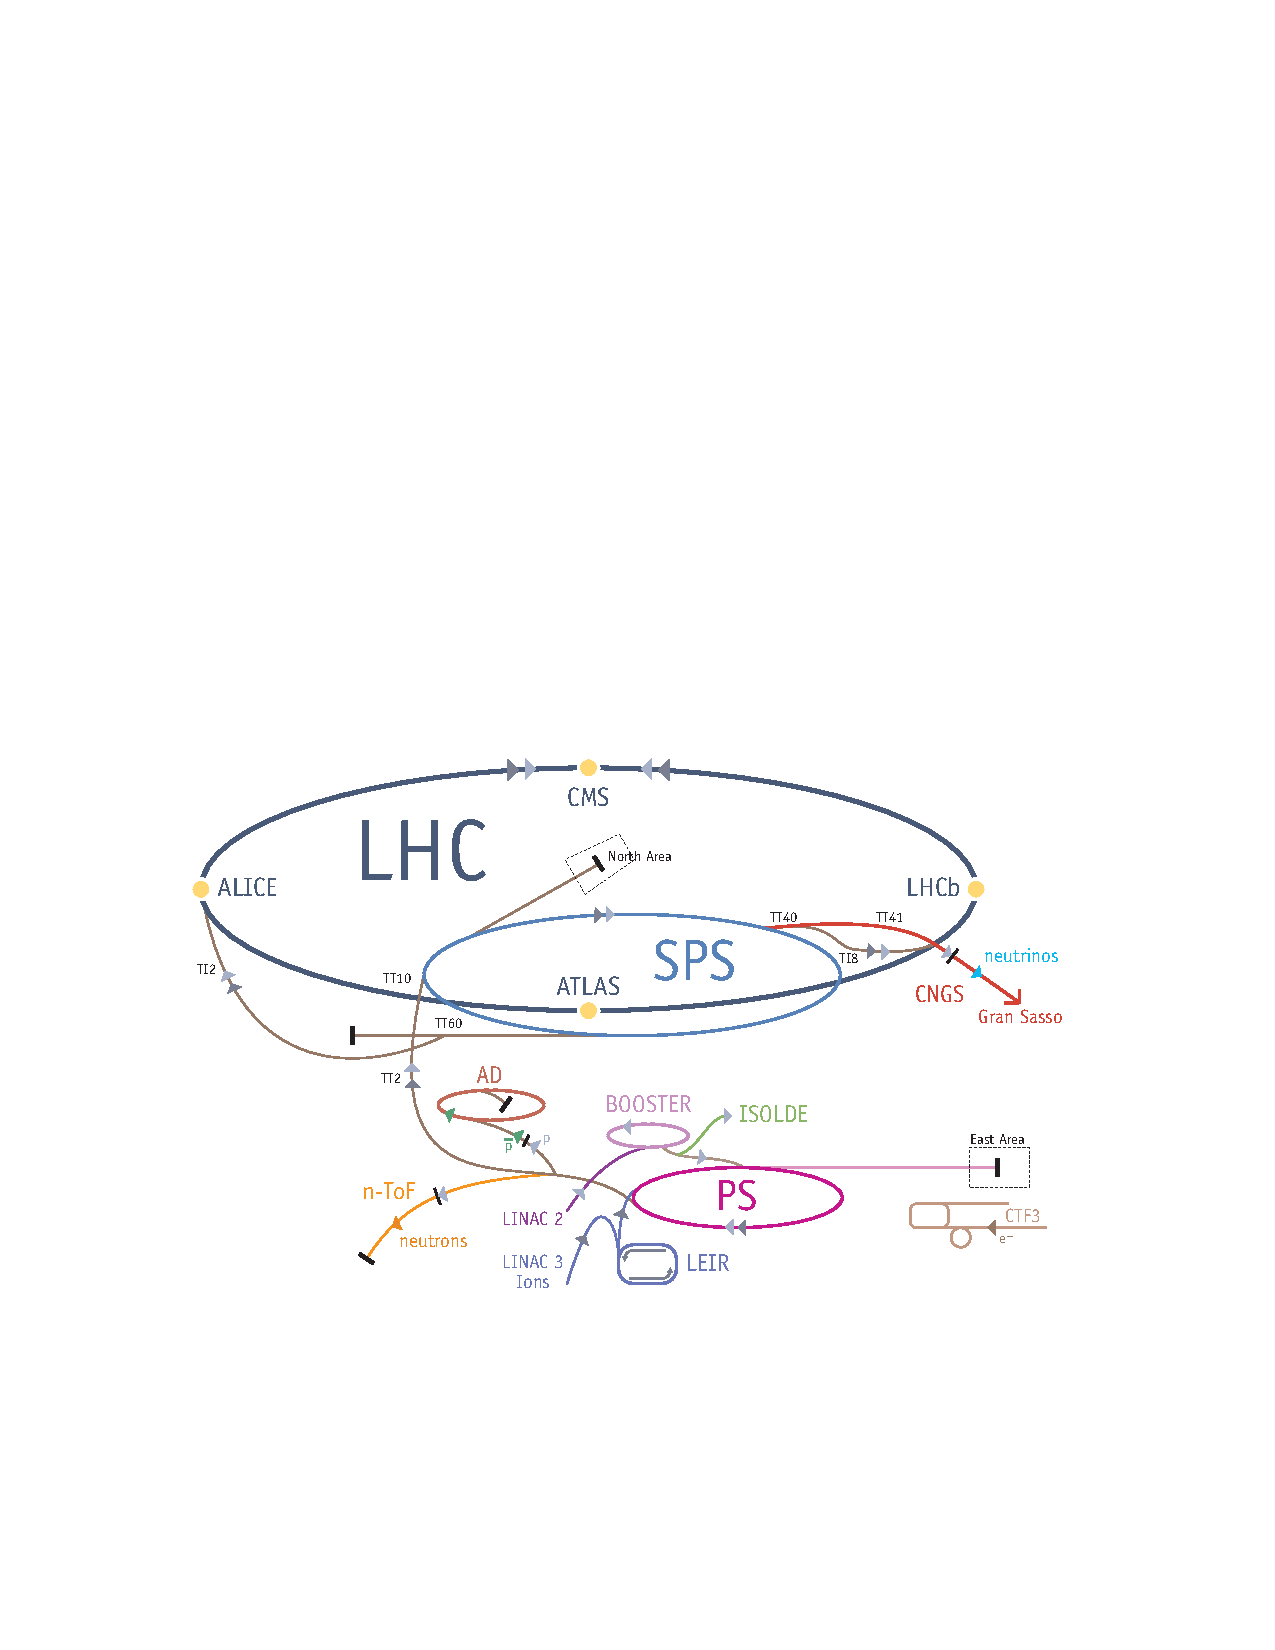
\includegraphics[angle=-0,width=0.8\textwidth]{2_LHC_and_CMS/pics/LHC.pdf}
\caption{Schematic view of the CERN accelerators and their connection
\label{fig:cern_accelerators}
}
\end{center}
\end{figure}

The LHC started its operation on 10 September 2008 and after only 9 days of operation a severe \emph{quenching} of about 100 dipole magnets, causing the release of around two tones of helium, forced the machine to stop and to address some design figures. The main cause of the accident was found to be in some of the electrical connections between magnets. In 2009 the machine became again operational with a reduced beam energy, allowing for less current to flow in the dipole magnets. The year 2010, after a careful ramp-up of the beam energies, saw the start of the LHC research program with collisions at a center-of-mass energy $\sqrt{s} = 7$ TeV, half of the designed one. During 2010 and 2011 the machine commissioning continued along with data taking improving the instantaneous luminosity and allowing for an increase of the beam energy to 4 TeV that took place in 2012. The LHC design specifications and achieved ones are summarized in table \ref{tab:lhc_figures}.

\begin{table}[h!]
   \centering
\begin{tabular}{c|ccccc}
\hline
Parameter & Design value&  Best value achieved \\ 
\hline
Beam energy   & 7 TeV & 4 TeV \\ 
Number of protons per bunch & 1.15$\times$10$^{11}$ & 1.5$\times$10$^{11}$ \\
Number of bunches & 2808 & 1368 \\
Crossing angle & 300~\si{\micro\metre} & 290~\si{\micro\metre} \\
Beam size & 17~\si{\micro\metre} & 20~\si{\micro\metre} \\
Emittance & 3.75 ~\si{\micro\metre} & 2.4~\si{\micro\metre}  \\
Peak luminosity & $10^{34}$~cm$^{-2}$s$^{-1}$ & 7.5$\times$10$^{33}$~cm$^{-2}$s$^{-1}$ \\
\hline
\end{tabular}
  \caption{Relevant LHC machine parameters. The design values are compared to the ones reached during the 2013 operations.}
  \label{tab:lhc_figures}                
\end{table}


The instantaneous luminosity,$\operatorname{\mathcal{L}}(t)$, is the number of particles per unit area per unit time available for collisions. For any given physics process the average number events is given by:

\begin{equation} 
	N_{ev} = \sigma\int\operatorname{\mathcal{L}}(t)\mathrm{d}t
	\label{eq:n_events}
\end{equation} 

where $\sigma$ is the cross-section for such process. While the cross section depends on the scattering process, the instantaneous luminosity is entirely derived from accelerator figures:

\begin{equation} 
	\operatorname{{\cal L}}(t) = \frac{N_p^2 n_b f_{rev} \gamma }{4 \pi \epsilon_{n} \beta^*} F
	\label{eq:lumi}
\end{equation} 

where $N_p$ and $n_b$ are the number of protons per bunch and the total number of bunches respectively, $f_{rev}$ is the rotation frequency, $\epsilon_{n}$ and $\beta^*$ describe the beam focusing at the interaction point, $\gamma$ is a relativistic factor and $F$ accounts for the crossing angle between the two beams. Although the number of bunches has always been less than half the design value during all the running period, the peak instantaneous luminosity has been only 30\% lower than the design one. This result was achieved by increasing the number of protons in each bunch and increasing the focusing of the beams, at the price of increasing the average number of proton collisions per bunch crossing, the so-called \emph{pileup}. This effect is displayed in figure \ref{fig:lhc_pileup} where the peak number of simultaneous interactions per bunch crossing recorded by the CMS detector is shown as a function of time.

\begin{figure}
\begin{center}
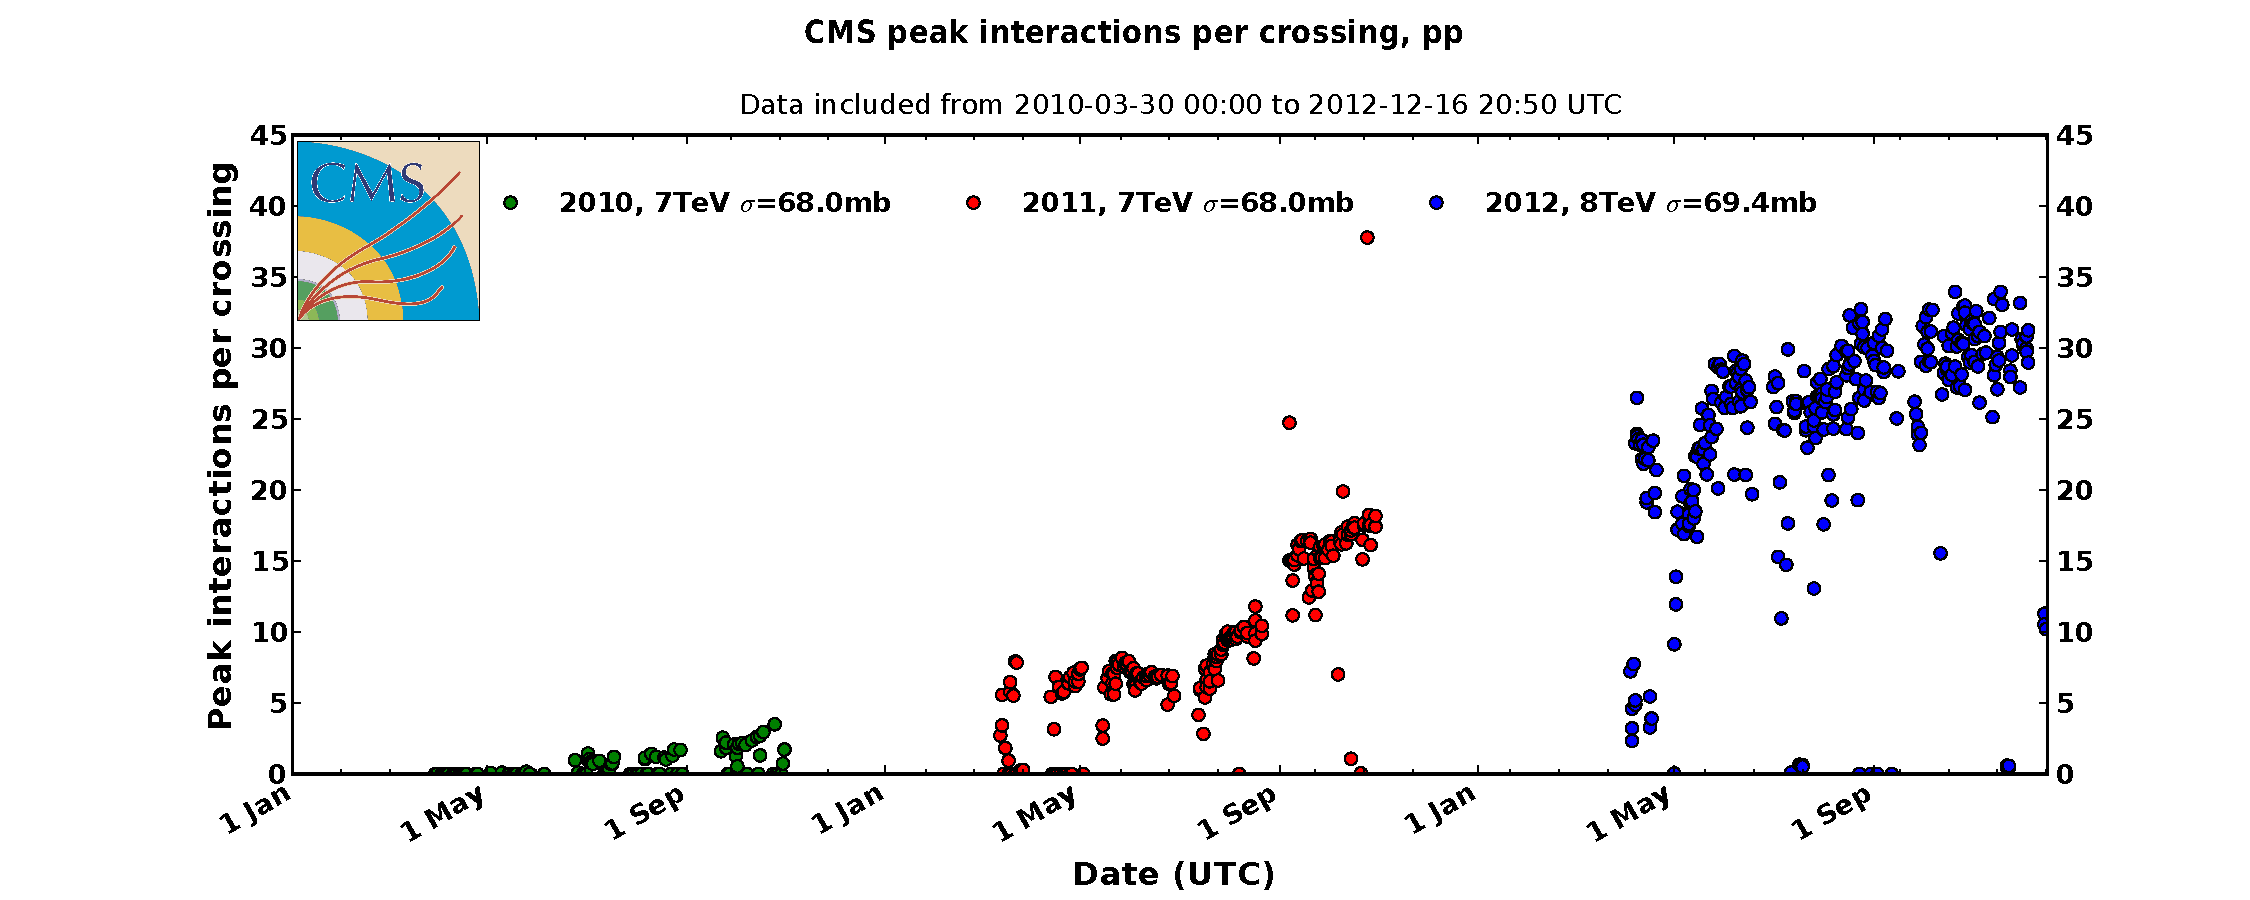
\includegraphics[angle=-0,width=\textwidth]{2_LHC_and_CMS/pics/peak_pu_pp.pdf}
\caption{Peak Interactions per Crossing versus time for p-p collisions (includes special runs), each point represents a Fill. This is shown for 2010 (green), 2011 (red) and 2012 (blue) data-taking.
\label{fig:lhc_pileup}
}
\end{center}
\end{figure}

The integrated luminosity is usually quoted as \L. During its operations LHC delivered 44.2~pb\Inv in 2010, 6.1~fb\Inv in 2011 and 23.3~fb\Inv at 8~TeV in 2012; Figure \ref{fig:int_lumi} shows the progress of the accelerator in terms of integrated luminosity.

\begin{figure}
\begin{center}
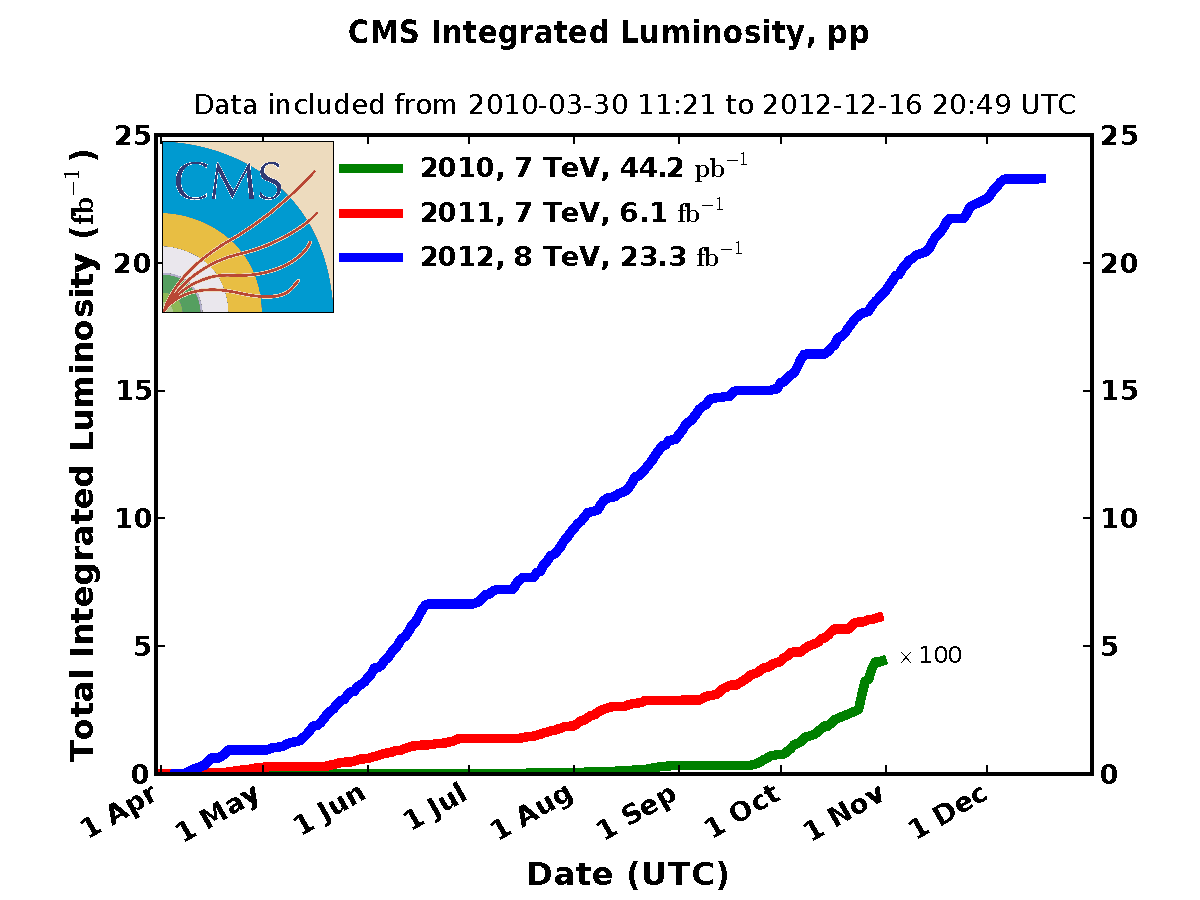
\includegraphics[angle=-0,width=0.8\textwidth]{2_LHC_and_CMS/pics/int_lumi.pdf}
\caption{Cumulative luminosity versus day delivered to CMS during stable beams and for p-p collisions. This is shown for 2010 (green), 2011 (red) and 2012 (blue) data-taking.
\label{fig:int_lumi}
}
\end{center}
\end{figure}


\section{The CMS detector}

The CMS detector is located in the LHC tunnel at point 5, near the French town of Cessy, between the Jura mountains and the Geneva lake.
 
The CMS experiment, together with ATLAS, is one of the two multi-purpose detectors operating at the LHC. Its primary task is to probe particle physics at the TeV scale looking for new phenomena and for the Higgs boson, the only missing piece to the SM puzzle. The experiment is also well suited to perform precision measurements of standard model processes and flavor physics studies. A heavy-ion program is carried on as well to probe QCD at very high energies and matter densities, trying to reproduce an environment similar to the conditions of the universe few instants after the Big Bang.

To carry out such ambitious research program the detector was designed to meet some baseline requirements:
\begin{itemize}
\item Good muon identification and momentum resolution over a wide range of momenta and angles with di-muon mass resolution of ~1\% at 100~GeV.
\item Ability to identify the muon charge without any ambiguity for muons momenta below 1~TeV
\item Good charged-particle momentum resolution, high tracking efficiency and resolution. This two figures are especially important for objects like \b-jets and tau leptons, where isolated charged hadrons and displaced vertices play a fundamental role. A high tracking resolution also plays a key role in assigning the tracks to the production vertex mitigating the effect of pileup.
\item Good electromagnetic energy resolution, with a di-photon invariant mass resolution of \~1\% at 100~GeV and wide geometric coverage with efficient photon and lepton isolation in high pileup conditions.
\item Hermetic hadronic calorimeter with fine transverse segmentation for good jet mass and missing transverse energy ($E_T^{miss}$) resolution. 
\end{itemize}

The total proton-proton cross section at 14~TeV is expected to be roughly 100~mb leading to an average of 20 pileup interactions with LHC design values. This value has been widely overcome during the 2012 data taking. The number of \emph{pileup} events together with the short 25~ns bunch spacing pose stringent requirements on the resolution, granularity and latency of the different subdetectors. The ability to resolve overlapping vertices and assign their respective track is of primary importance. A fast trigger system is also required to reduce the event rate from the design collision rate of 40~MHz to 300Hz which can be permanently stored.

In order to meet all these requirements CMS has been built with a 4~T NbTi superconducting solenoid magnet with an inner diameter of 6 m. Inside the magnet a large silicon tracker, the largest of its kind, is housed to track charged particles with the required resolution. Around the tracker, but still within the solenoid field, a lead-tungstanate electromagnetic calorimeter (ECAL) and a brass-scintillating sampling hadron calorimeter (HCAL) are installed. Inside the 1.5~m thick iron return yoke of the magnet four muon stations are installed. They consist of several layers of drift tubes or cathode strip chambers complemented by resistive plate chambers. A schematic view of a transverse CMS slice is presented in figure \ref{fig:cmsdet}

\begin{figure}
\begin{center}
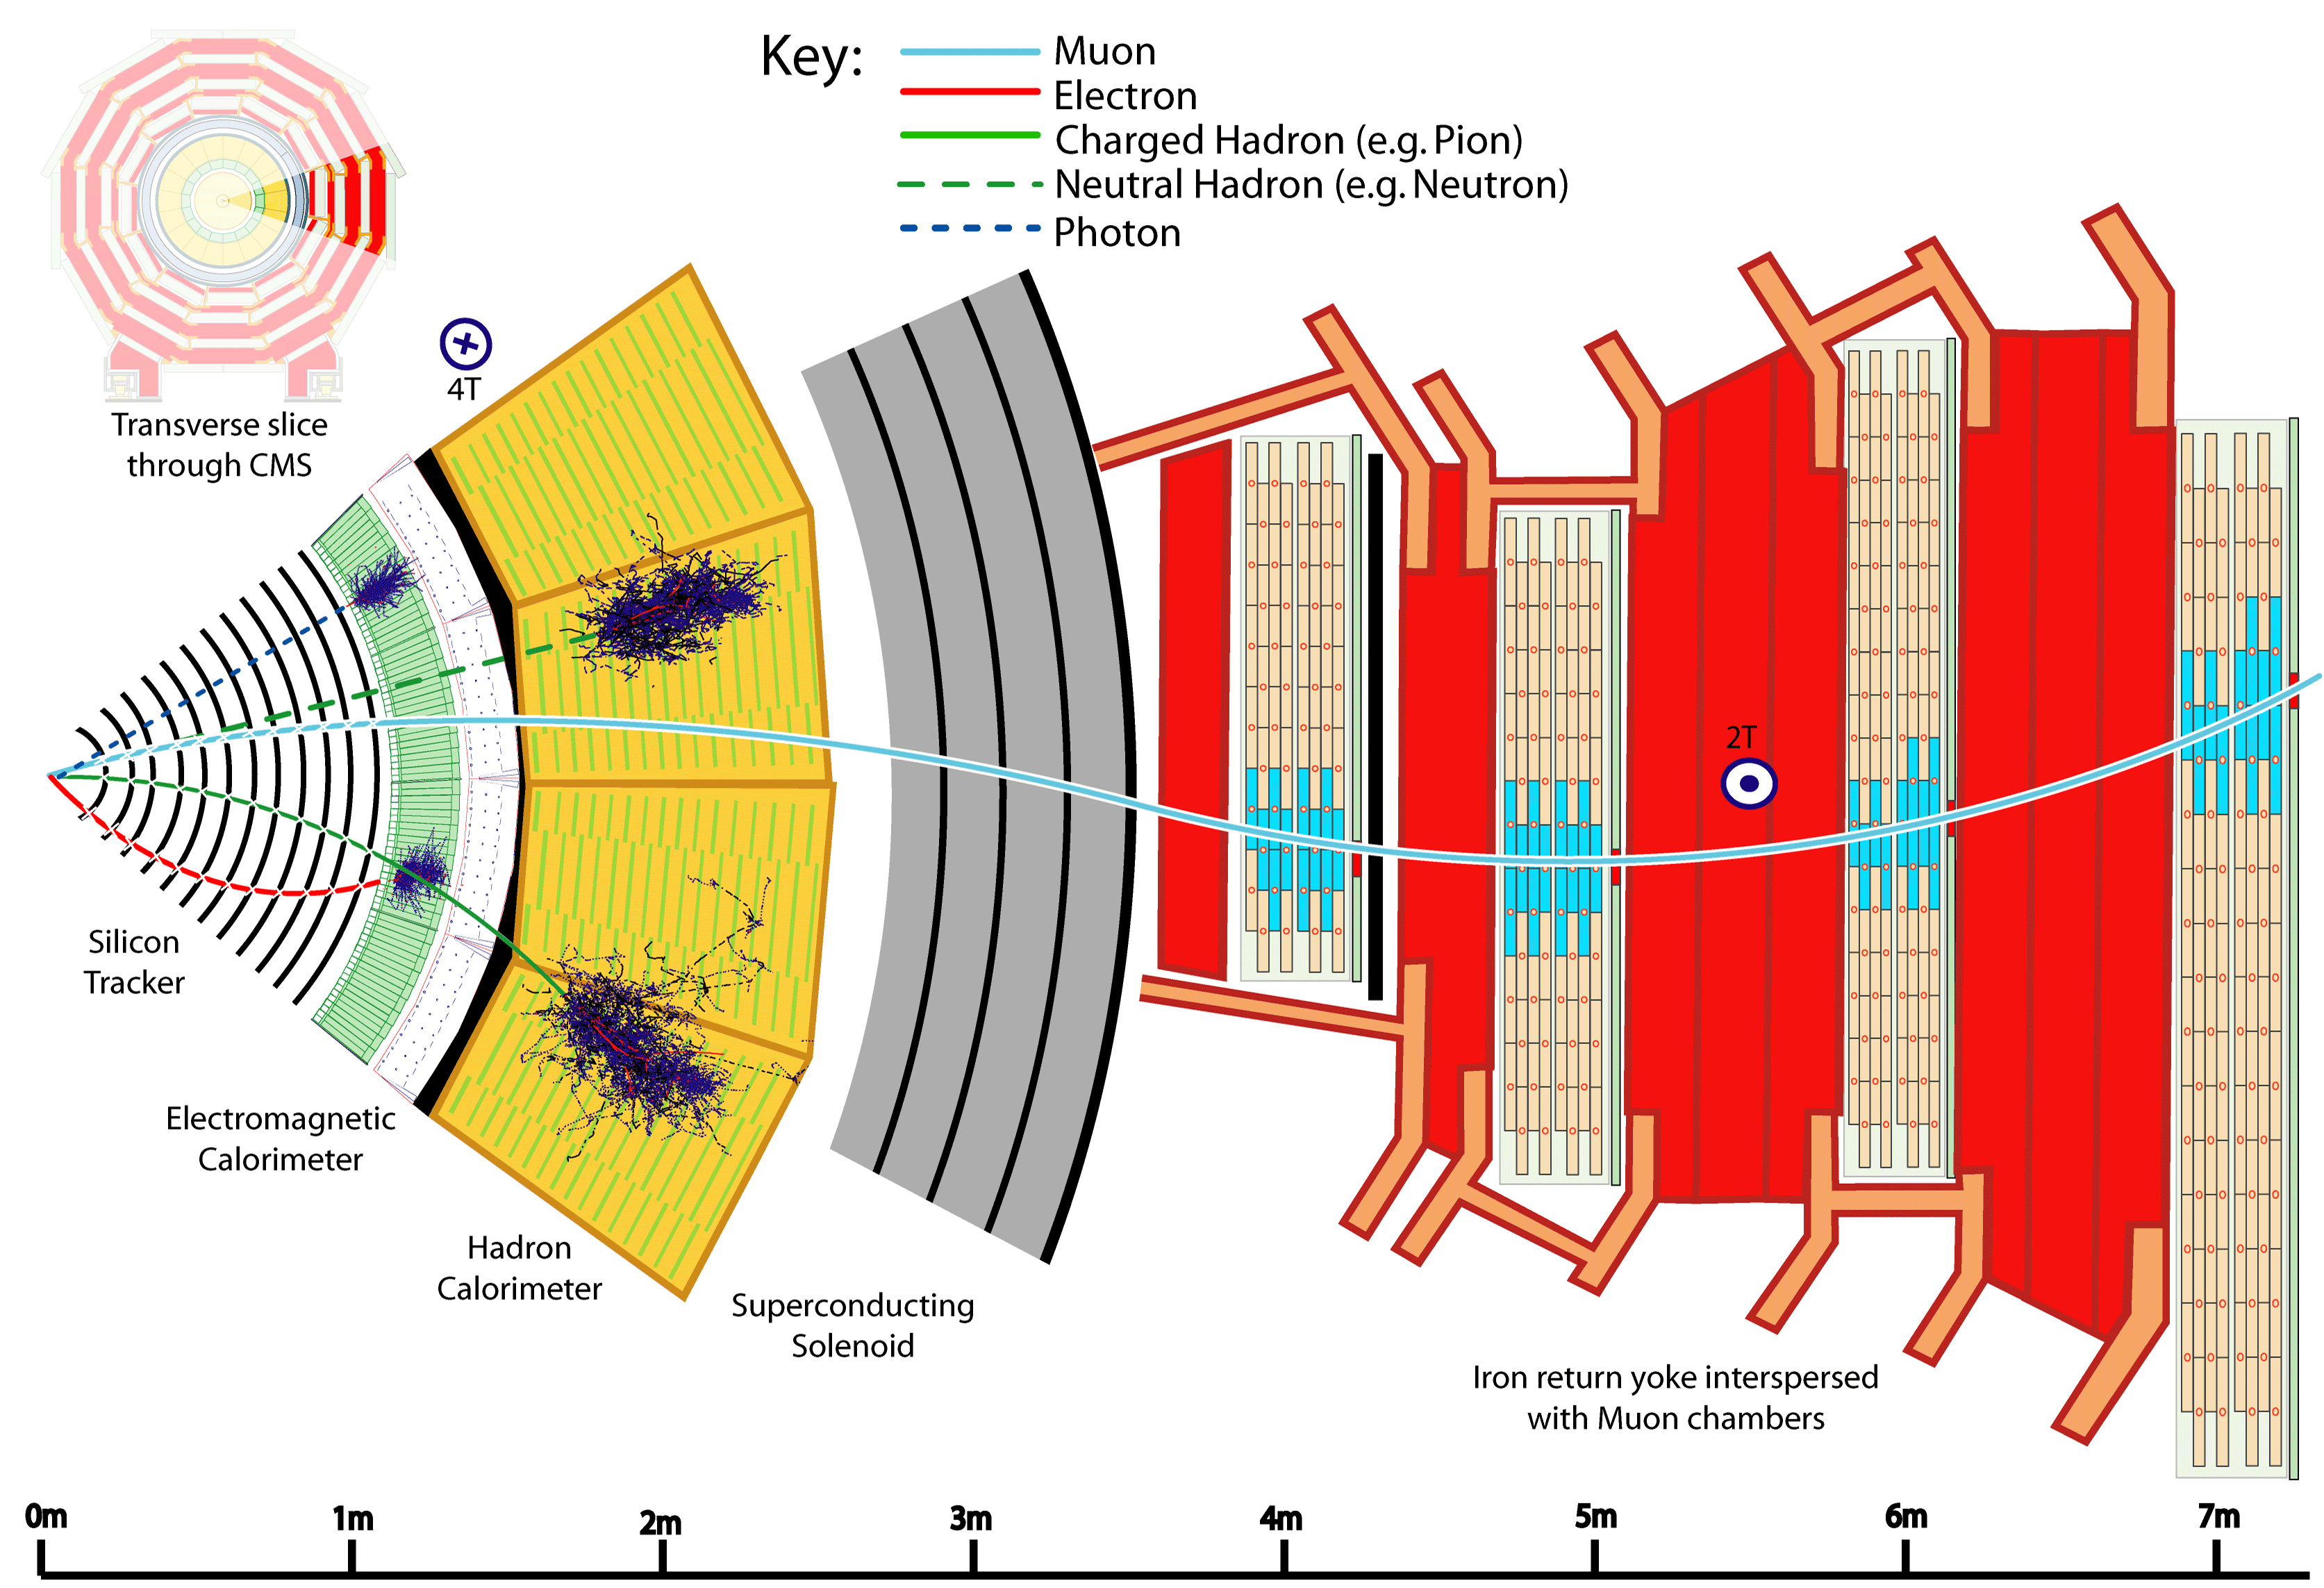
\includegraphics[angle=-0,width=0.8\textwidth]{2_LHC_and_CMS/pics/CMS_Slice_HD.png}
\caption{transverse slice of the CMS barrel section showing the trajectory for different particles with and the signal deposed in each subdetector.
\label{fig:cmsdet}
}
\end{center}
\end{figure}


\paragraph{The coordinate system}
chosen for CMS sets the $y$ axis vertical pointing upwards and the $x$ axis horizontal pointing towards the center of LHC, therefore the $z$ axis is placed along the beam line pointing in the direction of the beam running anti-clockwise or towards the Jura. An additional set of polar coordinates is used to describe the $xy$ plane in the form of radius $r$ and angle $\phi$, while the angle $\theta$ is measured with respect to the positive $z$ axis direction. Usually the polar angle $\theta$ is replaced by the \emph{pseudorapidity}, defined as $\eta=-\ln \tan(\theta/2)$, is Lorentz invariant for boosts along the $z$ axis and therefore comes very handy when describing processes whose longitudinal boost is unknown. The three-dimensional angular distance is also replaced by its Lorentz-invariant $\D R=\sqrt{\D\phi^2+\D\eta^2}$, where $\D\eta$ and $\D\phi$ are the $\eta$ and $\phi$ coordinate differences of two points.

\subsection{Inner Tracker}
\label{sec:inner_tracker}

The inner tracker provides the essential spatial informations needed to reconstruct charged tracks as well as primary and secondary vertices. A schematic view of the inner tracker is shown in figure \ref{fig:tracker}. To cope with the very high track density and to provide the best spatial resolution, the innermost part of the tracker is based on silicon pixel technology. The pixel detector, displayed in figure \ref{fig:pixel}, is composed of three cylindrical layers at radii of 4.4, 7.3 and 10.2 cm complemented by four disks  in the forward/backward region. The total active area of the pixel detector is roughly of 1 m\sq~and its angular acceptance covers $|\eta| \leq 2.5$, providing three bi-dimensional measurements over the full acceptance. The pixel cell size is 100 $\times$ 150 \u m\sq. High hit resolution is achieved thanks to the sharing of the ionization charge between neighboring pixels due to the solenoidal magnetic field. To enhance this effect in the forward wheels the sensors are placed in a turbine shape. The analogue read-out and charge sharing allow for a 9-33 \u m resolution \cite{trackingpaper}. 

The pixel detector can be extracted from the rest of the tracker to allow easy access for maintenance without interfering with the rest of the detector. This feature is particularly important due to the high radiation dose that the first layers of the pixel detector sustain, requiring additional maintenance.

\begin{figure}
\begin{center}
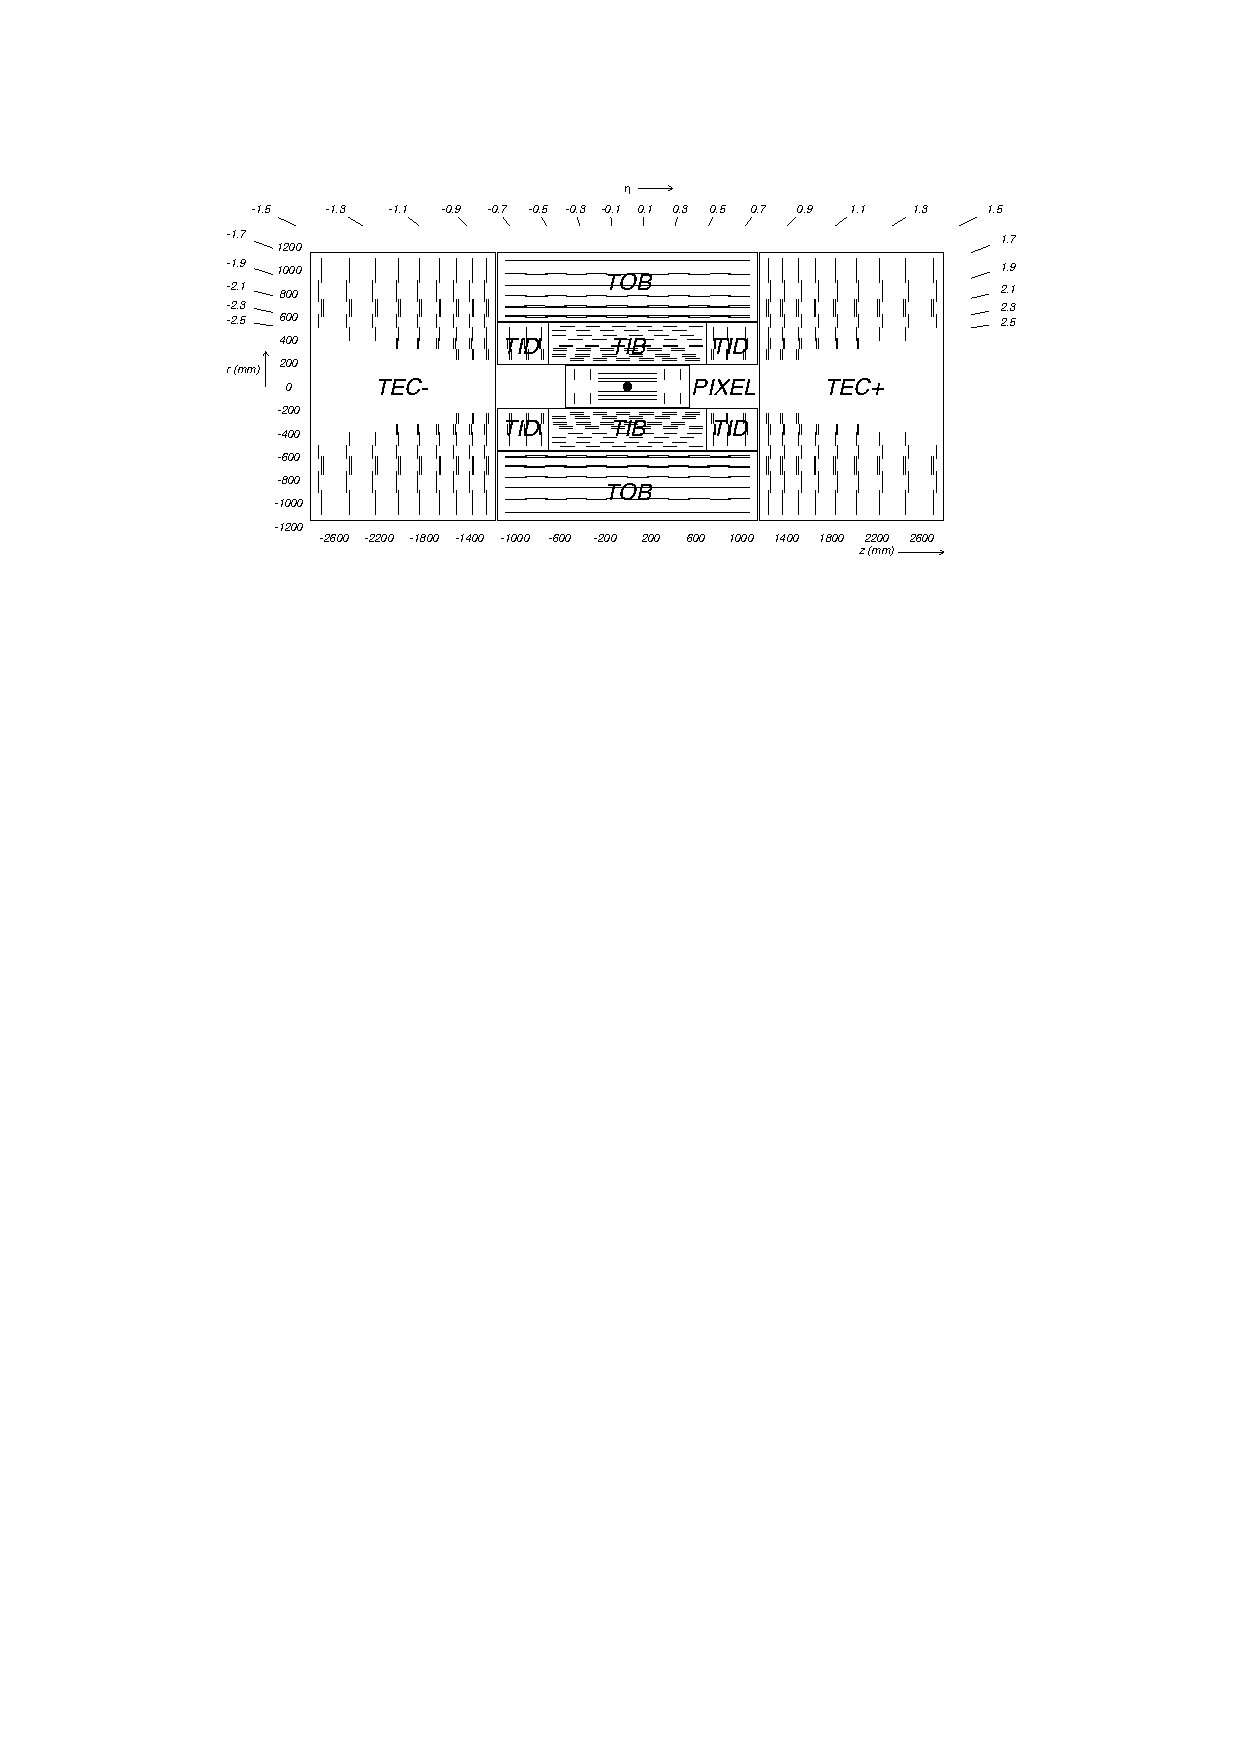
\includegraphics[angle=-0,width=0.8\textwidth]{2_LHC_and_CMS/pics/trkxsec.pdf}
\caption{Longitunal cross section of the CMS tracker with pseudo rapidity coverage. 
\label{fig:tracker}
}
\end{center}
\end{figure}

\begin{figure}
\begin{center}
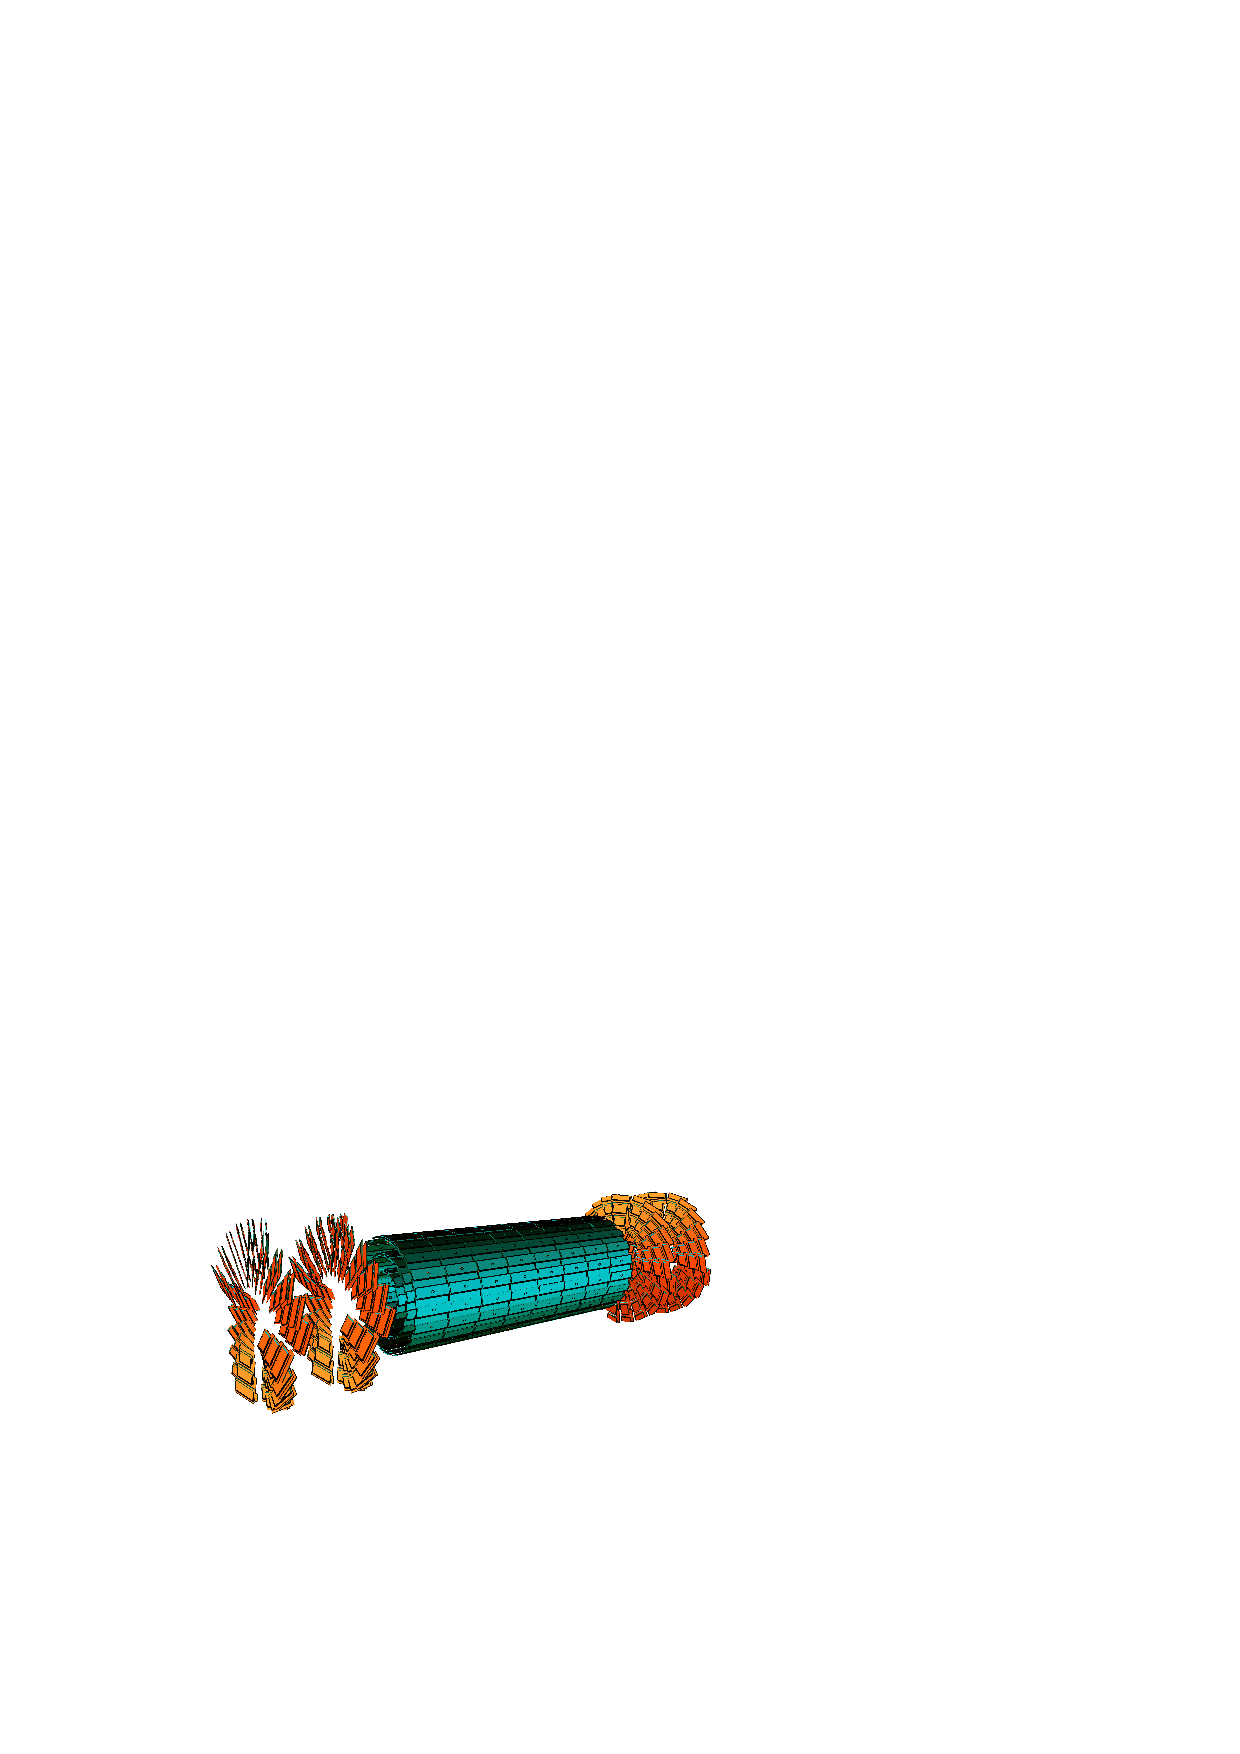
\includegraphics[angle=-0,width=0.8\textwidth]{2_LHC_and_CMS/pics/pixelfull.pdf}
\caption{Three dimensional sketch of the CMS pixel detector, barrel modules in blue and endcap wheels in orange.
\label{fig:pixel}
}
\end{center}
\end{figure}

The outer layers of the tracker are made of silicon strip detectors and further divided into four sections: Tracker inner and outer barrel (TIB and TOB), tracker inner disks (TID) and tracker endcaps (TEC), as illustrated in figure \ref{fig:tracker}. TIB and TID are located at radii between 20 and 55 cm from the beam line. They consist of four barrel layers and three disks at each end. The sensors are made of 320 \u m thick silicon with a strip pitch that varies from 80 \u m in the innermost barrel layer to 140 \u m in the outermost disks. The combination of TIB and TID delivers up to four transverse measurements. The TIB-TID sections are surrounded by the TOB, which fills the remaining space up to a radius of 116 cm from the beam line. It consists of six barrel layers of 500 \u m thick sensors with a strip pitch of 183 \u m for the first four layers and 122 \u m for the remaining two. The TEC is located in the end-cap region, for radii larger than 20 cm and $|z| > 118$ cm. It consists of nine disks composed by up to seven concentric rings of strip sensors. The thickness and the strip pitch of the sensor vary depending on the distance from the beam line. 

Intrinsically strip sensors only provide one dimensional spatial information ($\phi$). To measure a second coordinate ($r$ for disks, $z$ for barrel), an additional set of sensors is mounted back-to-back with a stereo angle of 100 mrad on the first two layers of TIB, TID and TOB and on layers 1, 2 and 5 of TEC. The strip tracker layout ensures about 9 hits in its acceptance with at least four of them being two-dimensional.

%temperatura?

\subsection{Electromagnetic Calorimeter}

The CMS electromagnetic calorimeter (ECAL) is located around the inner tracker. It is divided into ECAL Barrel (EB) covering the pseudo rapidity range $|\eta| < 1.479$ and ECAL Endcaps (EE) which cover $1.479 < |\eta| < 3$. 
The calorimeter consist of 68\,524 scintillating lead tungstanate (PbWO$_4$) crystals readout by photomultipliers. 

The choice of lead tungstanate was driven by its high density yielding a short radiation length (0.89 cm) and small Moliere radius (2.2 cm) together with the radiation hardness and fast response, with 80\% of the light yield emitted within 25~ns. To keep the calorimeter as hermetic as possible the crystals have truncated pyramidal shape with one of the longitudinal faces left unpolished to moderate the non uniform light collection across the crystal length that this peculiar shape causes. Each crystal covers about $0.0174 \times 0.0174$ in $\eta-\phi$ plane and is oriented pointing towards the nominal interaction point with a slight misalignment to mitigate the effect of the crystal surface on photon detection. Each crystal is read-out by either a pair of avalanche photodiodes (APD) in the barrel or by vacuum phototriodes in the endcap. Both the devices can operate in high magnetic fields with little or no efficiency degradation and showed good radiation resistance.

A pre-shower detector is installed in front of the ECAL endcap, with the purpose of discriminating between real photons and in-flight \piz decays and to enhance the angular resolution of both electrons and photons. The pre-shower detector consists of a double-layer lead-silicon calorimeter, with the lead initiating the shower and the silicon strip detector placed after each radiator measuring the deposited energy and shower profile with high granularity.

\subsection{Hadronic Calorimeter}

The hadronic calorimeter (HCAL) serves two purposes: it measures the energy of charged and neutral hadrons from the p-p interaction while stopping them, thus allowing only muons to pass through and avoiding large quantities of energy being deposited inside the superconducting magnet. As most of the other subdetectors HCAL is divided in a barrel section (HB), covering the acceptance region with $|\eta| < 1.3$, and an endcap section (HE) covering $1.3 < |\eta| < 3$. Both parts are located inside the superconducting solenoid. HCAL is a sampling calorimeter with brass passive plates, in which the hadronic shower begins and develops, interspaced with active plastic scintillator measuring the shower profile and the energy deposited. 

The scintillator is segmented both in $\eta$ and $\phi$ to provide the necessary granularity. Each scintillating tile is connected to the readout by a wavelength-shifting fiber that runs in a groove machined in the tile itself. Such fiber is thermally spliced to a clear fiber carrying the emitted light to a hybrid photodiode (HPD). The HPDs consist of a photocathode kept at high voltage. Electrons emitted by the photocathode are accelerated in the short distance (\~3 mm) that separates the cathode from a silicon pixelated anode which amplifies the signal. These devices were chosen due to their high dynamic range, their high gain ($O(2000)$) and the possibility to work in a magnetic field.

The effective thickness of the calorimeter in terms of interaction length, $\lambda_I$, spans in the barrel from a minimum of 5.82 $\lambda_I$ at $\eta=0$ to a maximum of 10.6 $\lambda_I$ at $|\eta| = 1.3$. The ECAL crystals add about 1.1 additional interaction lengths. The total thickness of the endcap calorimeters, including in the ECAL crystals, is about 10 $\lambda_I$.

Due to the limited stopping power of HB, especially in the central rapidity region, an additional hadronic calorimeter is placed outside the solenoid magnet (hadron outer or HO) with the function of \emph{tail catcher}. The HO consists of one scintillating station (two for the most central region) exploiting the solenoid itself ( and the first return yoke in case of the second station) as absorber. This additional detector extends the total thickness of the HB to a minimum of $11 \lambda_I$.

\subsection{Muon System}

Muon detection and trigger are of prime importance in CMS as many new physics processes may manifest through decay chains involving muons. Among those, the decay of a Higgs boson into $\Z\Z^*\To4\mu$ stands out as one of CMS's flagship analyses and one of those leading to the discovery of the Higgs boson announced on July 4$^{th}$, 2012 \cite{Chatrchyan:2013lba}. For this reason a redundant system of three different kinds of detectors is used to track muons in CMS. 

The muon system, whose scheme is shown in figure \ref{fig:mudet}, is housed in gaps between the return yoke of the solenoid magnet in the outermost region of the experiment. It consists of a Drift Tube (DT) tracking system in the barrel and multi-wire proportional chambers in the end-cap. In addition, a set of Resistive Plate Chambers (RPC) is located both in the barrel and in the endcap regions, providing a better time resolution  at the cost of coarser spatial resolution. 

\begin{figure}
\begin{center}
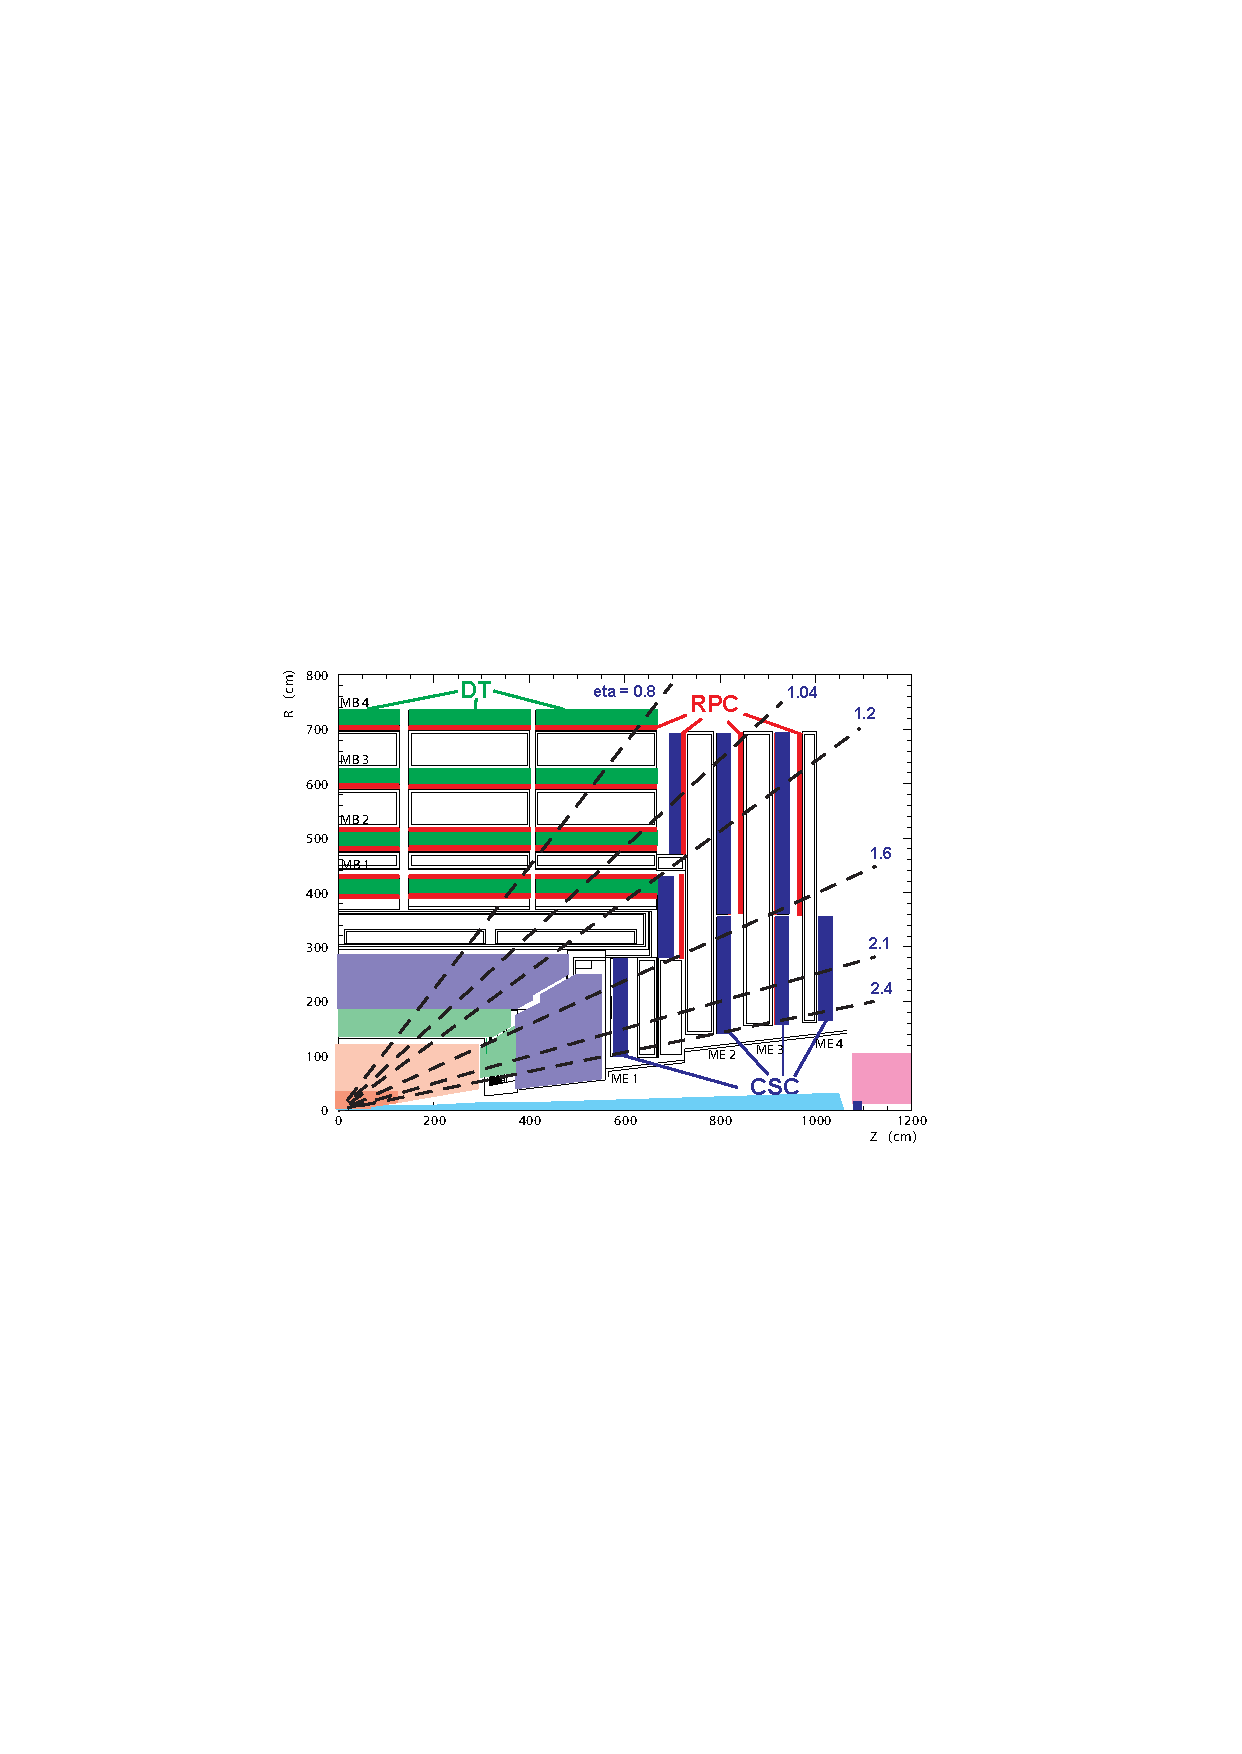
\includegraphics[angle=-0,width=0.8\textwidth]{2_LHC_and_CMS/pics/mudet.pdf}
\caption{Longitudinal cross-section of the CMS detector showing the location of the muon system.
\label{fig:mudet}
}
\end{center}
\end{figure}

\subsubsection*{Drift Tubes}

Drift tubes identify and track muons in the barrel region ($|\eta| < 1.2$) where the rate is below 1 Hz/cm\sq ~and residual magnetic field less than 1 T allowing the usage of this technology. Four stations are located at increasing distance from the beam line. The first three stations are equipped with two \emph{super-layers} (SL) providing a measurement of $\phi$ and one SL measuring the $z$ coordinate, as can be seen in figure \ref{fig:dt_module}, representing one DT module. In the last two stations the SL measuring the $z$ coordinate is missing. 

\begin{figure}
\begin{center}
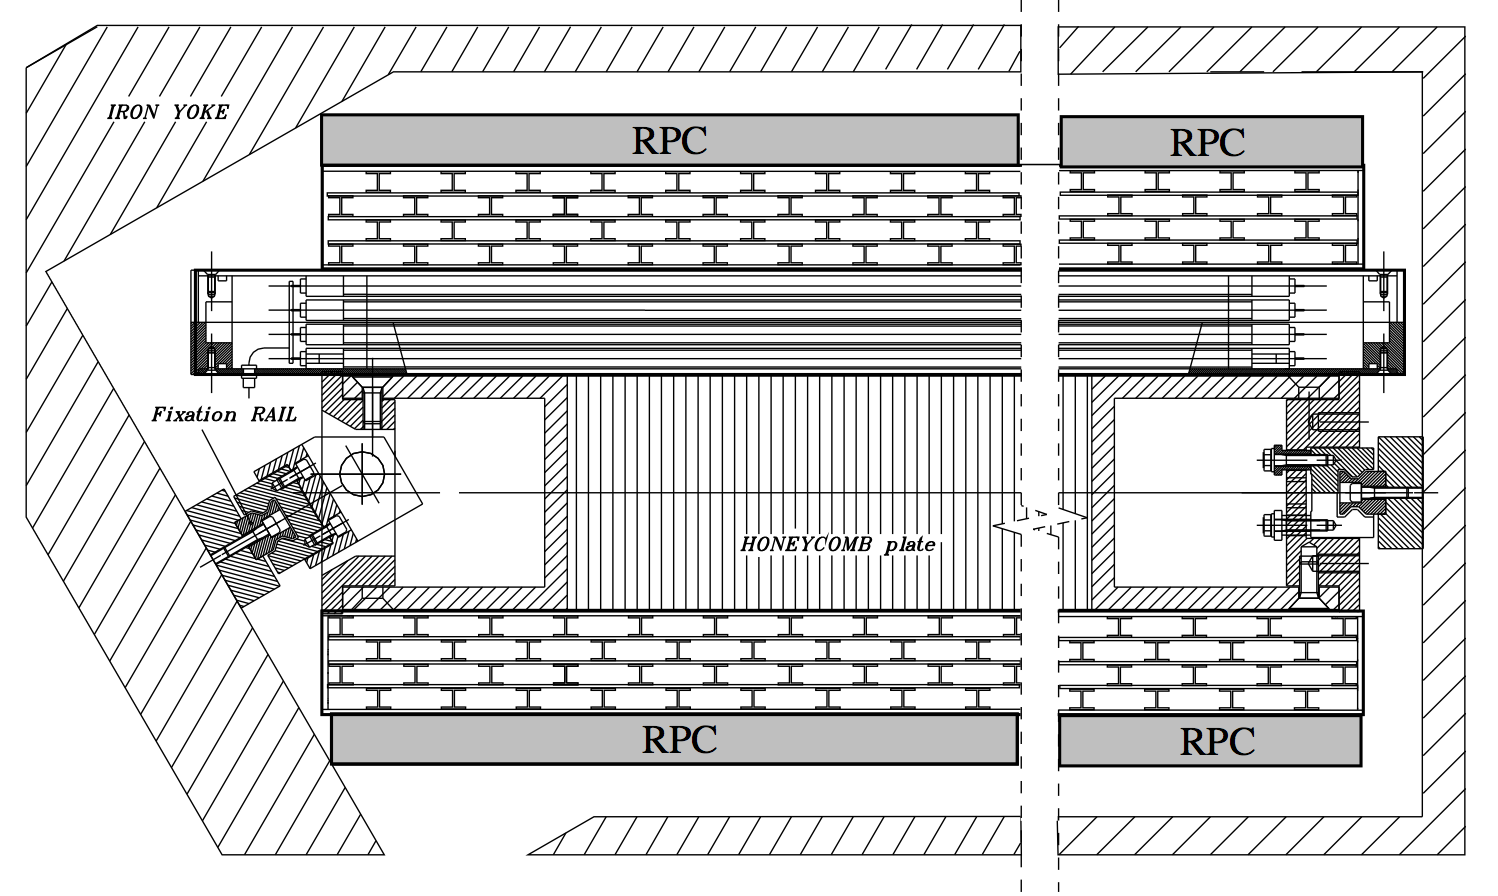
\includegraphics[angle=-0,width=0.8\textwidth]{2_LHC_and_CMS/pics/cms_dt.png}
\caption{Cross-section view of a DT module.
\label{fig:dt_module}
}
\end{center}
\end{figure}


Each SL is made of four stacked layers of tubes staggered by half a cell. This configurations eliminates blind spots and allow for an easy measurement of the muon crossing time by averaging the drift times. Each tube has a rectangular cross-section of $13\times42$ mm\sq ~and is filled with a gas mixture of 85\% Ar and 25\% CO$_2$, leading to a maximum drift time of 380 ns. Each SL has a spatial resolution of about 200 \u m and a time jitter below 5 ns.

\subsubsection*{Cathode Strip Chambers}

The front wheels of the solenoid return yoke are instrumented with multi-wire proportional chambers. Each module has trapezoidal shape and cover either $10\deg$ or $20\deg$ in $\phi$ forming a full disk perpendicular to the beam axis ($r-\phi$ plane). Each of these chambers has the cathode segmented radially in strips (hence the name Cathode Strip Chamber, CSC) of constant $\Delta\phi$ and wires running perpendicular to the strips with spacing of 3.2 mm. 

This design allows to cope with the much higher rate with respect to the barrel and with non uniform and non null magnetic field. 

This detector provides at least three measured points in its acceptance ($1.2 < |\eta| < 2.4$) with a design resolution of approximately 2 mm at trigger level and around 200 \u m after offline reconstruction.

\subsubsection*{Resistive Plate Chambers}

Dual-gap RPC's provide a redundant set of spatial measurements particularly important for trigger purposes, given their response time much shorter than 25~ns. The layout chosen by the CMS collaboration consist of six RPC stations in the barrel and three in the endcaps. RPC stations are placed in proximity (before or after) each CSC or DT station. The first two DT station have two RPC, one before \emph{and} one after, in order to provide at least four position measurements even for low-$p_T$ muons which might not reach the outer stations. Each chamber is operated in avalanche mode and consist of two gaps sharing a segmented pick-up read-out in between, allowing to operate at lower voltages (and therefore lower noise) for the same gain. 

\subsection{Trigger}

As previously said, during the operations LHC delivered an interaction every 50 ns leading to a 20 MHz frequency, half of the design one.
This frequency is well above the storage capabilities of the most modern technologies that allow to accommodate few hundreds of events per second. The inclusive p-p cross-section is hugely dominated by low-$x$ QCD processes that are of no or little interest for this experiment. This leads to the obvious necessity of a fast-logic to isolate events of some interest for the experiment's physics program while rejecting the others. This event selection of logic, usually referred as \emph{trigger}, is divided in the CMS experiment in two stages: the \emph{level one} (L1) trigger and the \emph{high level trigger} (HLT). 

The L1 trigger decision is based on a coarse reconstruction of the event performed by custom electronics largely mounted directly on the detector. The maximum processing time (called \emph{latency}) is 3.2 \u s. During this time the event is stored on the detector electronics in pipelined memories. Due to timing constraints only inputs from the calorimeters and from the muon system are processed. In this trigger process, the calorimeter segmentation is reduced into the so-called \emph{trigger-towers}. Calorimeters provide to the decision logic a set of important physics variables like the missing transverse energy ($E_T^{miss}$), the scalar sum of the transverse hadronic activity ($H_T$), the number of jets above different energy thresholds and the locations of towers compatible with a \emph{minimal ionizing particle} (MIP) and its isolation. Electron and photon identification is also performed looking at the jet hadronic over electromagnetic energy ratio ($H/E$) and cluster shape, performed with the aid of a look-up table. Muon information is mainly provided by DT and CSC subdetectors complemented by the sheer time resolution of RPC for bunch crossing assignment as well as ghost-tracks removal. Muons trajectories are roughly reconstructed by the detector dedicated electronics and then sent to an additional module that merges the information coming from the different stations and subdetectors to assess the transverse momentum  and charge. These informations are complemented by those coming from the calorimeters providing isolation values.

The final decision is taken by modules located outside the detector. These modules exploit FPGA's to achieve fast response while allowing for modification of the algorithms to cope with the evolution the instantaneous luminosity or new physics demands. The maximum output frequency for L1 is 1 kHz.

Once the L1 trigger decision is made the full event is read out from the detectors buffers and sent to the online \emph{Data Quality Monitoring} (DQM) and to the HLT farm, consisting of over a thousand commercial processors working in parallel. During the HLT decision, a simplified version of the CMS offline event reconstruction is performed. Time consuming tasks such as tracking are performed only around the objects that caused the L1 trigger to fire and more complex algorithms like \b-tagging and \t~identification are performed with a simplified version. During this trigger stage, decisions are taken on the basis of more complex algorithms and a more refined reconstruction, which allows to reduce the event rate to roughly 300Hz, within the storage and processing capabilities of the CERN facilities. Being completely software-based, the HLT is far more flexible and fast evolving than the L1 trigger, allowing to cope with the fast changing machine conditions during 2010 and 2011 runs and achieving a level of refinement beyond the most optimistic forecasts made at the start-up.

Once the event is accepted by the HLT too, it is transferred to the CERN computing center for storage and reconstruction.

\section{Data storage and processing}

Events recorded from the detector are stored in \emph{RAW} format, a data format that contains all the digitalized output of the single subdetectors and L1 and HLT information. In order to be useful for physics analysis the trajectory and the nature of the particles originated in the event must be inferred from the hits stored in the RAW event. This process is usually called event reconstruction and is the topic of the following chapter. The CMS detector produces about 15 TB of data for each day of operation.

The reconstruction of collected and simulated data is too CPU and storage demanding to be delegated to a single facility. In order to evenly spread this effort through different computing facilities in various parts of the world, a new computing model has been created. The \emph{world wide computing grid} \cite{Malecki:2005gn} allows for fast transfer and de-localized computing throughout the world, allowing to cope with the huge demands that the LHC experiments need to smoothly operate. 

In some sense the grid can be seen as an extension of the batch queue system where the user submits jobs to a single machine, whereas, in this case, he submits them to clusters of machines, that then take care of submitting those jobs in their peculiar batch queue implementation. Computing facilities are organized in a hierarchical structure called tiers, starting from the facility that receives the data from the detector, called Tier0, scaling to smaller and smaller facilities up to Tier3's which provide limited computing and storage for local groups. In this system secure access to the resources is ensured by a system of certificates spawning children proxies of limited lifetime.

%displayed
%presented
%illustrated
\chapter{Event reconstruction in CMS}

While traversing the different detector layers, the particles produced in the physics collisions deposit energy in the detectors that is amplified and recorded. Most sub-detectors are capable of measuring the particle position as well as the deposited energy. Each collision event results in a series of position measurements in the different layers of the tracking detectors plus energy clusters in the calorimeter. The reconstruction algorithms takes care of ``connecting the dots'' and provide the most complete and accurate description of the event as it originated from the collision. In this task the execution time plays an important role, as the algorithms used by the reconstruction cannot be excessively resource demanding. In this chapter we will briefly describe the techniques used to reconstruct the events recorded by the CMS detector starting from the most basic objects and then moving towards the most complex ones. Finally, we describe the \emph{Particle Flow} algorithm that gives a global description of the event. In the final section of the chapter we will describe in detail the hadronic tau reconstruction, which plays a fundamental role in this work, and the techniques used to measure its efficiency, a measurement which has been carried as part of the doctoral work presented in this thesis.

\section{Track reconstruction}

The signals recorded by the innermost sub-detector, the inner tracker ( see section \ref{sec:inner_tracker}), are used to reconstruct the trajectory and momenta of the charged particles originating from the proton collisions as well as the location (vertex) where these interactions occurred. An accurate and detailed description of the tracking algorithms can be found in Ref. \cite{cms_trk_11_01}.

The innermost part of the tracker, made of silicon pixel detectors, records the hit position together with the charge deposited in the detector. Due to the Lorentz drift the charge deposited by a ionizing particle is shared between neighboring pixels, improving the position resolution of the detector. The outer part of the tracker, made of silicon strip detectors, generally records only the $\phi$\ coordinate of the hit except for few layers where an additional strip module rotated by a 100 mrad stereo angle allows for a bi--dimensional measurement of the hit positions.

Due to huge number of hits recorded in each event, reconstructing the tracks corresponding to the hits is not trivial. The strategy adopted by the CMS collaboration employs a \emph{combinatoric track finding} (CTF) approach with very stringent requirements on the tracks, thus finding the easiest ones to reconstruct first. These requirements are progressively loosened in several iterations. After each iteration the hits used to build the tracks are removed from the pool of available hits. This procedure, called \emph{iterative tracking}, allows to achieve a very high tracking efficiency with low fake rate and acceptable resource usage. 

At the beginning of each iteration the tracks are seeded from triplets or doublets of hits in the tracker. In case of doublets an additional constraint on the beam-spot is used to reduce the fake rate. Only 2D hits are used at this stage to build track seeds. A first evaluations of the main track parameters (\pT and 3D impact parameter) is also performed at the seeding step. Track seeds not satisfying the minimal requirements for that iteration are discarded.

Track seeds are then propagated ``inwards'' (in the direction of the nominal interaction point) and ``outwards'' (in the direction of the calorimeter) the seeding layers in order to search for compatible hits that can be assigned to the track. The analytical propagator used at this stage assumes uniform magnetic field in between the two detector layers and neglects multiple scattering effects. New candidate hits are added to the track candidate and its parameters are updated by a \emph{Kalman Filter} \cite{Fruhwirth:1987fm}. Only the track candidates satisfying a certain fit quality (evaluated with the $\chi^2$) are retained. This process, known as \emph{track finding}, is repeated until the innermost and outermost layers of the tracker are reached by the track propagation. During this process the Kalman Filter retains only the latest and most accurate evaluation of the track parameters and the addition of a new hit does not require re-evaluating the full trajectory, saving a large amount of computing time. Track candidates emerging from this process are cleaned, merging those candidates sharing the majority of the hits. Mutually-exclusive hits (hits belonging to the same detector layer) are arbitrated according to the $\chi^2$\ goodness of the track fit.

Track candidates found during the track finding step are then fitted by the means of Kalman filter and smoother. This choice is as accurate as a standard fit, but more effective from the computational point of view. Trajectory parameters are evaluated both starting from the innermost hit in the tracker and from the outermost one and then averaged, avoiding any bias due to the recursive nature of the Kalman Filters. During this process the more refined Runge-Kutta propagator is used to take into account un--homogeneities of the magnetic field and the effect of materials. Track candidates are finally selected according to the quality of the fit. Hits belonging to the tracks produced by this last step are removed from the collection of available hits and a new iteration with different seeding conditions and track requirements begins. 

A total of six iterations is performed on each event, the first ones are aimed at reconstructing most of the tracks originating from the main vertex, while the following ones focus on reconstructing tracks coming from displaced decays of long lived particles and from vertices in peripheral regions of the interaction region.

The solution adopted for the track reconstruction provides a tracking efficiency exceeding 90\% over a wide \pT spectrum as shown in Fig. \ref{fig:tracking_eff}.

\begin{figure}[h!]
\begin{center}
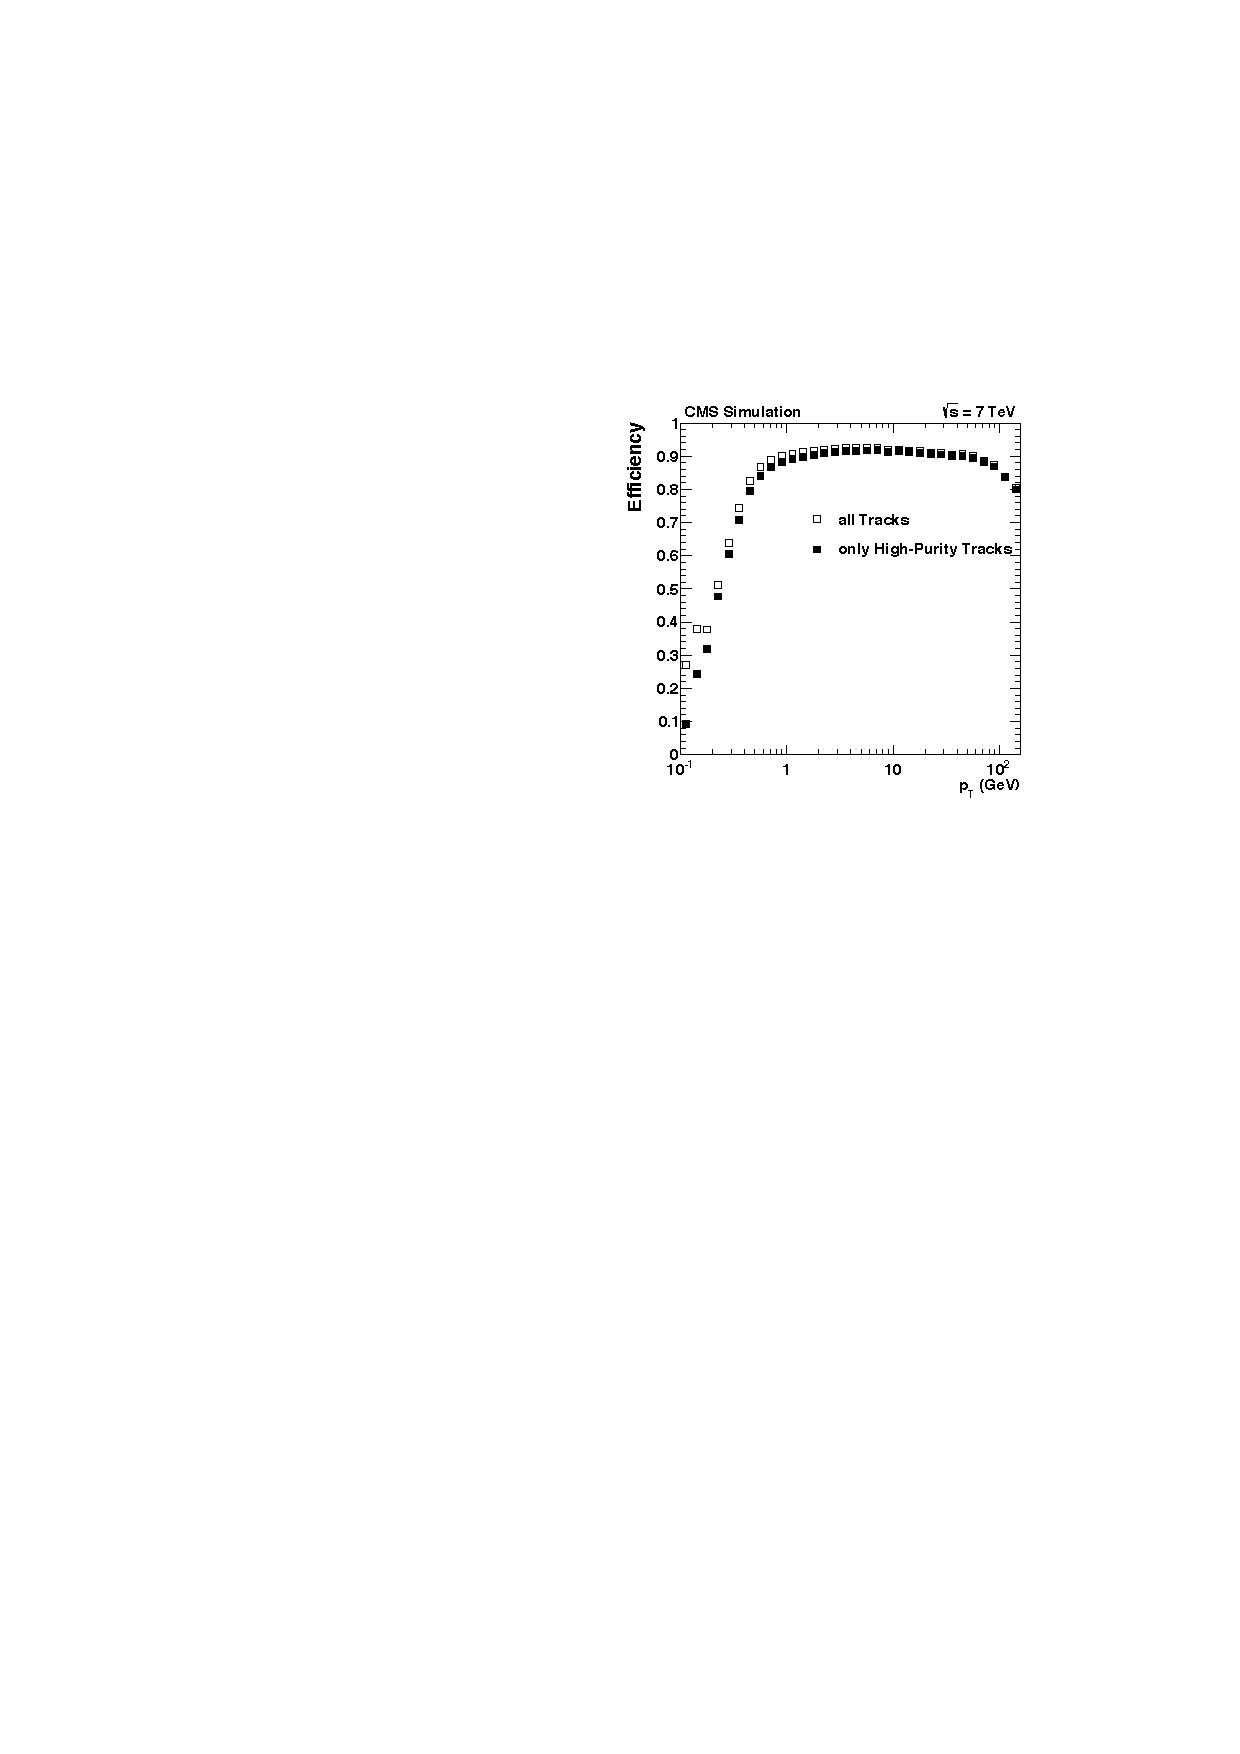
\includegraphics[width=0.5\textwidth]{3_Evt_Reconstruction/pics/trackeff.pdf}
\caption{Efficiency of the track reconstruction algorithm as a function of the particle $p_T$. It is obtained using a sample of simulated top pair events with an average number of simultaneous p-p collisions equal to 8.  
\label{fig:tracking_eff}}
\end{center}
\end{figure}


\subsection{Reconstruction of muon tracks} 

Muons can be considered a special case of the tracking algorithm, given the dedicated tracking system located outside of the solenoidal magnet. This additional lever arm allows to achieve a very good momentum resolution above 200 GeV, where the inner tracker resolution begins to degrade. 
In CMS, the muon reconstruction is seeded both by the tracker and by the muon chambers. In the former case every track above a few GeV is considered a potential muon and a tentative match with hits in the muon system is performed. If the match succeeds, the track is refitted and it acquires the status of \emph{tracker muon}. In the latter approach, a track is reconstructed by the CTF using only hits in the muon system. These tracks are seeded by track segments reconstructed by L1 trigger electronics. These \emph{standalone muons} tracks are then propagated inside the inner tracker to match with a track. As in the previous method, a successful match causes the full trajectory to be refitted and the combined object is called a \emph{global muon}. Tracker muon reconstruction is obviously more efficient than the latter for low \pT muons as they may not leave enough hits in the muon chambers to preform a full track reconstruction, but it also suffers from a larger fake rate. The two muon collections are then merged into a single one, removing double candidates.

\section{Vertex reconstruction}

Vertices are reconstructed in CMS by a \emph{Deterministic Annealing} (DA) \cite{IEEE_DetAnnealing} clustering algorithm. The tracks used during vertex reconstruction are preselected according to their transverse impact parameter with respect to the beam spot, the number of hits and the $\chi^2$\ of the track fit, to ensure that only good prompt tracks are used in the vertex reconstruction. No requirement on the track \pT is imposed in order to maximize the reconstruction efficiency in events with very little transverse momentum transfer between the colliding protons, called \emph{minimum bias} events, which compose the majority of of pile-up interactions.

Once the tracks are selected, further computations are based on the $z$\ coordinate of the points of closest approach between the tracks and the beamspot ($z_i^T$), and its uncertainty ($\sigma_i^Z$). In the DA framework the vertex position is evaluated by minimizing a modified version of the $\chi^2$\ with an additional term inflating $\sigma_i^Z$\ of each track. This parameter is called ``temperature'' since it behaves as the physics observable in statistical mechanics, with the  $\chi^2$\ acting as free energy.

Starting from one single vertex located centrally, the temperature is iteratively lowered and the free energy term minimized for each iteration. As the temperature lowers, some tracks start being incompatible with the only available vertex and a better minimum is found by splitting the tracks in two subsets belonging to two different vertices. This splitting is done ``softly'', i.e. each track can be assigned to multiple vertices with a weight between 0 and 1. With the lowering of the temperature the weights tend to assume values increasingly closer to the end-points.

The annealing process is continued down to a minimal temperature, which ensures good vertex resolution and very limited risk of splitting true vertices. After this threshold no more vertex splittings are allowed, but the temperature is still iteratively reduced and potential outliers in the vertex fits are removed. Once the final temperature ($T=1$) is reached, tracks are assigned to the corresponding vertices if their weight is greater than 0.5 as spurious weights may still be different from zero. 

Each set of tracks assigned to a vertex is then fitted with the \emph{adaptive vertex filter} algorithm \cite{CMS_NOTE_2007-008}, consisting of an iterative weighted Kalman Filter, to evaluate the vertex position with the best possible precision.

Such refined technique allows to achieve a vertex reconstruction efficiency between 98\% for cluster  of two or three tracks and 100\% for the rest, with a negligible fake rate of about 1\%. The vertex resolution for clusters of few tracks is about 200 \um both in the transverse and longitudinal plane, rapidly decreasing to an asymptotic value of about 20 \um as more tracks are used to compute the vertex position.

\section{Electron and photon reconstruction}

Both electrons and photons are reconstructed starting from ECAL clusters, which are seeded from local maxima in the energy deposition. A cluster size of $5\times5$\ crystals on average contains 95\% of the energy of an unconverted photon. This average value is considerably reduced in the real environment due to photons converting into $e\+e\-$ pairs when traversing the material in front of the calorimeter and the $e\+e\-$ pairs being separated in the $r-\phi$\ plane by the magnetic field. Photon conversions result in wider energy clusters, elongated in the $\phi$ direction. Similar arguments can be made for electrons and positrons, that emit a sequence of \emph{bremsstrahlung} photons as they approach the surface of the calorimeter. In order to recover this energy the $5\times5$\ clusters are grouped together in \emph{superclusters} (SC), elongated in the $\phi$\ direction. A more detailed description of the clustering algorithm can be found in \cite{CMS:2006tdr1}.

The bremsstrahlung process and its intrinsic non-Gaussian energy emission makes the Kalman filter approach unsuitable. It is replaced by the Gaussian Sum Filter (GSF) \cite{gsf} which handles the energy loss properly. The usage of the GSF and its larger propagation uncertainties makes a tracker-only approach unfeasible both for reasons of computation time and of low track purity. In order to reduce the amount of fake tracks, the seeding step starts from ECAL superclusters from which two track candidates are propagated inside the tracker under both charge assumptions looking for two compatible hits in the pixel detector. After the seeding, the tracking process continues as described in the previous section with the GSF substituting the KF. This modified version of the tracking algorithm is also used to correctly identify photon conversions within the tracker volume, looking for highly displaced vertices compatible with a massless state and matching a broad supercluster in the electromagnetic calorimeter.

Several variables are used to discriminate between fake and real electrons, such as the supercluster shape, its energy and location with respect to the impact position in the calorimeter, expected from the measured track parameters, and the presence of energy deposits in the hadronic calorimeter. All these variables are combined to perform the electron identification. Several working points, both with cut-based and MVA-based approach are available. The latter exploits TMVA's \cite{TMVA} Boosted Decision Tree (BDT) implementation to separate electrons from charged hadrons and photons. The BTD behavior has been trained on real electrons selected from a $\Z \To ee$ sample and fake ones from a $\Z \To ee + Jets$ one.

Photon identification is based on the same supercluster quantities as the electron identification but doesn't require a charged track to be matched to the ECAL energy deposit.  

\section{Particle Flow}

The redundancy of signals that particles traversing the CMS detector leave in multiple sub detectors is exploited by the \emph{Particle Flow} (PF) algorithm in order to improve the overall description of the event. The particle flow method furthermore allows for cross-cleaning of spurious signals and achieve to a global description of the event.

Building blocks for the PF algorithm are the different types of track collections plus the calorimeter energy deposits. Local maxima in the calorimeter deposits serve as seed for ``topological clusters'' which are grown iteratively, by adding adjacent cells with an energy deposit above a customizable threshold. After the clustering stage the algorithm links the different blocks according to their position in the $\eta-\phi$\ plane. Tracks are considered linked to calorimeter clusters if the track trajectory propagated to the average shower depth falls within the cluster boundaries, within some distance that accounts for resolution effects. Calorimeter clusters are linked if the center of the inner cluster fits within the boundaries of the outer one. The radial ordering of the linking step reflects the higher spatial resolution of the inner calorimeters (pre-shower, ECAL, HCAL). After the linking step is completed, the algorithm starts building the final objects, starting with muons. Each global muon that has a combined momentum measurement compatible with the track reconstructed in the inner detector is called a \emph{PF muon}. The corresponding track is removed from the track collection and an estimate of the associated energy deposit in the calorimeter is also removed from the list of linked clusters. Electrons are the second category of objects that is built with the procedure detailed above. Tangents to the electron trajectory in correspondence of the tracker layers are propagated to the ECAL in search for bremsstrahlung photons. If the electron candidate passes the selection cuts a \emph{PF Electron} is created and the track as well as the ECAL deposits linked to the track are removed. A tighter selection is performed on the remaining tracks, requiring that the tracker \pT resolution is smaller than the calorimetric energy resolution. This requirement is found to reject about 0.2\% of tracks in hadronic jets, 90\% of which being fake tracks. 
%Nonetheless this requirement was found to be a issue for hadronic tau reconstruction for high \pT taus and a custom modification was introduced. 
The algorithm finally exploits the redundancy in the transverse momentum measurement performed by the tracker and by the calorimeter to build \emph{PF charged hadrons, photons and neutral hadrons}. The PF algorithm operates under the assumption that all the hadrons (charged and neutral) traversing the detector are pions. Photons and neutral hadrons are produced from the calorimetric energy in the clusters once the energy of the linked tracks is subtracted. In the rare case that a calorimetric cluster has a total energy that is incompatible and lower than the sum of the linked tracks a dedicated procedure aimed at recovering mis-reconstructed muons is performed, recovering muon identification efficiency at no expense of increasing the fake rate.% Finally, to each PF object is assigned a PDG identification number and a mass.

\subsection{Muon identification}

The muon identification step in the PF reconstruction is necessary in order to suppress the hadronic punch-through, i.e. very energetic charged pions passing through the hadronic calorimeter and reaching the innermost muon station. %, and the in--flight decay of pions. 
The work presented in this thesis uses the tight working point of the PF muon identification, also referred to as ``PFTight'' within CMS.
The corresponding selection cuts are:

\begin{itemize}
\item The candidate muon must be reconstructed both as global and PF muon;
\item The normalized $\chi^2$\ of its global track fit must be less than 10;
\item There must be a least one DT or CSC hit included in the global fit;
\item At least two muon stations must be matched to the candidate;
\item The associated tracker track must have a transverse impact parameter $\mathrm{d}_{xy} < 2$\ mm and a longitudinal distance $\mathrm{d}_{xy} < 5$\ mm;
\item It must have at least one hit in the pixel detector and more than 5 hits in the whole tracker.
\end{itemize}

\subsection{Isolation}

A large fraction of the leptons produced in a proton-proton collision are due to the decay of mesons within jets. In order to separate these leptons from the ones which originate from the decay of a heavy resonance it is important to quantify the \emph{isolation} of the lepton, i.e. the amount of hadronic activity surrounding the lepton trajectory in a cone of a certain radius. The isolation can be computed separately with respect to charged and neutral particles. 

While the effect of pileup can be easily removed from the charged isolation by using only tracks associated to the selected primary vertex, the same is not possible for the neutral component. In fact calorimeters do not have sufficient spatial resolution to uniquely associate each cluster to a certain interaction vertex. The contribution of pileup to the neutral isolation is estimated by computing the energy deposited by charged tracks from pileup (i.e. not assigned to the hard-scatter vertex) and correcting it for a factor 1:2 to account for the amount of neutral energy with respect to charged one. This estimate is called \emph{$\Delta\beta = I^{pileup}_{charged}/2$}. To limit the effect of statistical fluctuations in the charged to neutral ratio on event-by-event basis the $\Delta\beta$\ correction is capped to the neutral isolation value. The \emph{relative isolation}, i.e. the isolation divided by the \pT of the object, can therefore be written as

\begin{equation}
I_{rel} = \dfrac{I_{abs}}{\pt} =  \dfrac{\sum{p_{T charged}} + \operatorname{max}(\sum{E_{T neutral}} - \D \beta, 0)}{p_T}.
\label{eq:db_rel_iso}
\end{equation}

\subsection{Jet clustering}

The particles reconstructed by the PF algorithm are clustered into jets using the \emph{Anti-kT} \cite{Cacciari:2008gp} algorithm. The Anti-kT belongs to the family of sequential recombination algorithms together with the Cambridge-Aachen and the kT algorithm \cite{Ellis:1993tq,Dokshitzer:1997in}. All these algorithms require the definition of the distance measure between two objects (in this case PF particles) and of the distance from the beam axis. In case of the Anti-kT algorithm, the distance between two objects is defined as:

\begin{equation}
d_{ij} = \operatorname{min}(\dfrac{1}{p_{Ti}^2},\dfrac{1}{p_{Tj}^2})\dfrac{\Delta R_{ij}^2}{r^2},
\end{equation}

where $r$\ is a constant parameter defining the size of the jet cone and $\Delta R = \sqrt{\Delta \eta^2 + \Delta \phi^2}$.
The distance of an object from  the beam is defined as:

\begin{equation}
d_{iB} = \dfrac{1}{p_{Ti}^2}.
\end{equation}

The algorithm starts with a high-\pT object used as seed and then it clusters around the seed all other objects until the minimum distance between the candidate jet and the closest object is larger than $d_{iB}$. One can show that this algorithm is infra-red safe, meaning that the jet shape and energy do not depend strongly on the energy of low--\pT particles clustered around a high \pT object. The Anti-kT algorithm gives rise to almost--conical jets of size $r$\ in angular aperture. Special cases are overlapping jets and jets with multiple high \pT objects within the angular acceptance.

The jets used in this work have been reconstructed with the Anti-kT algorithm with a radius parameter $r=0.5$ and their energies have been corrected to account for non-linear response of calorimeters and other instrumental effects \cite{Chatrchyan:2011ds}.

Pileup interactions deposit a considerable amount of energy in the detector. %this energy can easily overlap among different vertices and 
Furthermore, the energy deposits due to different pileup interactions may overlap and be misinterpreted by the Anti-kT algorithm as one hard jet. The CMS experiments exploits a combination of tracking and jet shape variables to discriminate between pileup jets and jets originating from the hard scattering. The information provided by these variables is interpreted by a BDT 
trained on simulated $\Z\To\mu\mu$ events \cite{CMS-PAS-JME-13-005}. The training is divided in four different $|\eta|$\ categories that reflect the resolution of tracking information and granularity of the calorimeters.

\subsection{Missing transverse energy}

%Most of the particles produced in a p-p collision leave a signal in at least one sub-detector except 
Neutrinos and other hypothetical (not yet observed) weakly--interacting particles that are neutral and stable leave no trace when traversing the detector and hence can not be directly reconstructed. Their presence can be inferred by utilizing the conservation of transverse momentum in the event. The observable quantifying an observed imbalance is called \emph{missing transverse energy} (\MET). It is computed as the negative vectorial sum of all the PF objects reconstructed in the event \cite{CMS-PAS-JME-13-003}: 

\begin{equation}
\vec{\cancel{E}_T} = -\sum^{PF\;obj.} \vec{p_{T}}
\end{equation}

The magnitude of the \MET is found to be underestimated for various reasons including thresholds in the calorimeter clustering and signal non-linearities. This bias is significantly reduced in case the correction to jet energies are included in the formula \cite{Chatrchyan:2011ds}, obtaining the ``type 1''-corrected \MET. The introduction of jet energy corrections (JEC) is performed by subtracting the vectorial residuals between all corrected and uncorrected jets found in the event:

\begin{equation}
\vec{\cancel{E}_T^{corr}} = \vec{\cancel{E}_T } - \sum_\mathrm{jets} (\vec{p}_\mathrm{T,jet}^\mathrm{corr}-\vec{p}_\mathrm{T,jet})
\label{eq:Type1MET}
\end{equation}

Additional corrections, named ``type 0'' and ``$\phi$'', correct for biases induced by pileup and by asymmetries in the $\phi$\ direction \cite{AN-13-233}.

\section{Tau reconstruction and identification}
\label{sec:tau_id}

Hadronic taus are one of the highest level objects reconstructed from CMS data and the last in the event reconstruction chain. The reconstruction and identification algorithm exploits all the detector capabilities and the Particle Flow algorithm to achieve a reconstruction efficiency close to 60\% with a sub-percent fake rate. The tau reconstruction algorithm used in CMS is called \emph{Hadron Plus Strip} (HPS) \cite{CMS-PAS-TAU-11-001,AN-14-008}. 

\subsection{Reconstruction}

Tau reconstruction is seeded from PF jets clustered by the Anti-kT algorithm with $r = 0.5$. In order to recover most of the photon conversions, the tau reconstruction algorithm clusters PF electromagnetic objects (electrons and photons) with deposited energy above 0.5 GeV in topological ``strips'' of size $0.05 \times 0.20$\ in $\eta$\ and $\phi$ direction, respectively. Strips satisfying a minimum transverse energy of 2.5 GeV are combined with the charged hadrons to form the tau candidate. The charged hadrons included in the tau reconstruction must satisfy the following requirements:

\begin{itemize}
\item $\pt > 0.5$\ GeV;
\item track fit $\chi^2 < 100$;
\item track transverse distance of closest approach to the PV $d_0 < 0.03$\ cm;
\item track longitudinal distance of closest approach to the PV $d_z < 0.4$\ cm;
\item At least three hits in the tracker.
\end{itemize}

The algorithm builds all possible combinations of hadrons plus strips matching one of the following decay modes:

\begin{enumerate}
\item \emph{single hadron}: corresponding to a single hadron and no strip.
\item \emph{hadron plus one strip}: the invariant mass of the pair has to be compatible with the $\rho$\ meson, $0.4 < M_{\tau \; candidate} < 1.3 \cdot \sqrt{\pt \mathrm{[GeV]} / 200}$\ GeV. The upper boundary of this window is limited at 1.3 (2.1) GeV for candidates with $\pt < 200 \, (> 800)$. The increasing window size accounts for resolution effects at high \pT.
\item \emph{hadron plus two strips}: the invariant mass of the triplet has to be compatible with the $\rho$\ meson, $0.4 < M_{\tau \; candidate} < 1.2 \cdot \sqrt{\pt \mathrm{[GeV]} / 200}$\ GeV. The upper boundary of this window is limited at 1.2 (2.0) GeV for candidates with $\pt < 200 \, (> 800)$.
\item \emph{three hadrons}: the invariant mass of the triplet must be compatible with the $a_1$\ meson, $0.8 < M_{\tau \; candidate} < 1.5$\ GeV. The tracks are required to be compatible with originating from the same vertex and to sum to unit charge.
\end{enumerate}

In addition the previous requirements, tau constituents are required to be contained within a cone of size 0.1, $3 / \pt \mathrm{[GeV]}$\ or 0.05 for tau candidate with $\pt < 30$ GeV, $30 < \pt < 60$ GeV and $\pt > 60$ GeV, respectively. If more than a tau candidate can be formed within the same jet only the candidate with the largest \pT is kept.

\subsection{Identification}

Hadronic tau decays reconstructed by the HPS algorithm are %identified according to their isolation within the seeding jet. 
required to be isolated in order to suppress fakes due to quark and gluon jets. Only charged hadrons with \pT above 1 GeV and photons with $E_T$\ above 1.5 GeV are considered when computing the isolation. To mitigate the effect of pileup the neutral isolation is corrected with the $\D\beta$\ method computed in a cone of $\Delta R = 0.8$ around the tau candidate. The mismatch in the size of the isolation cone ($0.5$) and the one in which the pileup contribution is computed (0.8) leads to a conversion factor from charged pileup to neutral pileup isolation of 0.4576 that is empirically found to make the tau identification efficiency insensitive to pileup.

Three working points are provided: loose, medium and tight, corresponding to isolation thresholds of 2.0, 1.0 and 0.8 GeV respectively.

%An MVA-based discrimination exploiting tau kinematic variables and isolation as well as transverse inpact parameter is also provided, but is not used in this work.

\subsection{Light lepton rejection}

The PF charged--hadron collection may contain a significant amount of electrons and muons that do not pass the selections to enter the PF electron and muon collections, and therefore are considered to be charged hadrons by the tau reconstruction algorithm. Electrons and muons from the decay of W and Z bosons are typically isolated. 
As a consequence, the background due to $e\To\tau_h$\ and $\mu\To\tau_h$\ fakes may be sizable. %The combination of this two effects causes a relatively large $e\To\tau_h$\ and $\mu\To\tau_h$\ fake rates, especially in the single hadron (muon and electrons) and in the hadron plus one strip (electrons only) decay modes. 
In order to reduce these backgrounds, dedicated discriminators against electrons and muons have been developed \cite{AN-12-417}.

\paragraph{Electron rejection:} The rejection of electrons is performed with the aid of a boosted decision tree. Tau candidates are classified into different categories depending on:

\begin{itemize}
\item The decay mode in which the tau candidate is reconstructed. Three decay modes are considered: single hadron, hadron plus one or two strips, and three hadrons. The three hadrons decay mode always passes the electron rejection discriminator;
\item Whether the hadron is associated to a track reconstructed by the GSF algorithm;
\item Whether a GSF electron candidate is reconstructed in the same direction as the tau candidate within a distance $\Delta R < 0.3$;
\item Whether the tau candidate is reconstructed in the ECAL barrel ($|\eta| < 1.479$) or endcap ($|\eta| > 1.479$).
\end{itemize}

All the possible combinations of the previous cases are considered, leading to a total of 16 mutually exclusive categories. Each category is trained separately using a mixture of  simulated events containing both signal and background processes: $\Z/\gamma^*\To\tau\tau$, $\Z/\gamma^*\To ee$, $\W\To \tau\nu$, $\W\To e\nu$, $t\anti{t}$, $H\To\tau\tau$, $\Z'\To\tau\tau$, $\Z'\To ee$, $\W'\To \tau\nu$, $\W'\To e\nu$. Events are considered as ``signal'' or ``background'' depending on whether the tau candidate is matched to a generator-level hadronic tau decay or an electron within a cone of size $\D R < 0.3$, respectively. 

%MVA training variables can be divided into four groups and are used in the training depending on the category whenever possible. The variables are summarized below.
The input variables to the BDT can be divided into four groups. The variables are:

\bold{Hadronic tau variables} (available for all categories):
\begin{itemize}
\item Invariant mass, \pT and \Eta of the tau candidate;
\item Ratio of ECAL to the sum ECAL plus HCAL energy deposits of the tau constituents;
\item Ratio of ECAL plus HCAL energy deposits of the tau constituents to the tau candidate \pT;
\item $\D\eta$\ between the tau candidate and the closest ECAL crack;
\item $\D\phi$\ between the tau candidate and the closest ECAL crack (used for candidates in the ECAL barrel only).
\end{itemize}

\bold{Strip variables} (available for taus reconstructed in the decay modes hadron plus one strip or hadron plus two strips only):
\begin{itemize}
\item $\sqrt{\pt^{\gamma} \cdot (\Delta\eta)^{2}}$\ and $\sqrt{\pt^{\gamma} \cdot (\Delta\phi)^{2}}$, 
  the \pT--weighted RMS of distances along $\eta$\ and $\phi$\ direction between all photons included in any strip and the charged hadron;
\item Fraction of $\tau_{h}$\ candidate energy carried by photons.
\end{itemize}

\bold{GSF track variables} (available only when the charged hadron is associated to a GSF track):
\begin{itemize}
\item $\ln (\pt)$, $\eta$ and normalized \chisq of the GSF track;
\item PF electron MVA output for the PF charged hadron;
\item $(N_{hits}^{GSF} - N_{hits}^{KF})/(N_{hits}^{GSF} + N_{hits}^{KF})$, where $N_{hits}^{GSF}$\ and $N_{hits}^{KF}$\ are the number of tracker hits associated to the GSF and KF tracks, respectively;
\end{itemize}

\bold{GSF electron variables} (only available in case a GSF electron is found near the hadronic tau candidate):
\begin{itemize}
\item The ratio between the total ECAL energy and the electron momentum measured at the IP;
\item Normalized \chisq, $\ln (\pt)$, $\eta$, \pT resolution ($\sigma_{\pt}/\pt$), and numbers of hits in the tracker of the electron GSF track;
\item The ratio between the bremsstrahlung photon energy as measured by the ECAL and by the track, $\sum E_{\gamma}/(P_{in}-P_{out})$, where $P_{in}$ is the momentum at the interaction vertex and $P_{out}$ is the one on the ECAL surface;
\item $F_{brem}=(P_{in}-P_{out})/P_{in}$, the ratio between the bremsstrahlung photon energy as measured by the track and the electron momentum measured at the IP;
\end{itemize}

Four working points are defined: \emph{loose }, \emph{medium}, \emph{tight} and \emph{very tight}, nominal efficiency ranging from 95\% to 80\% in steps of 5\% and corresponding decreasing $e \To \tau_h$ fake rate. %For each working point a set of different thresholds for each category is obtained by a recursive optimization. Starting from the tightest possible value (threshold set at 1 for each category), the algorithm progressively lowers the requirement in the category that allows for the highest gain in efficiency over fake-rate. The procedure is repeated until the desired fake rate is obtained.

\paragraph{Muon rejection:} uses a cut-based approach, looking for segments in the muon chambers near the direction of %muon signatures in the surroundings of 
the tau. Two working points are provided:

\begin{itemize}
\item \bold{Loose}: tau candidates are rejected if track segments in at least two muon stations are found within $\Delta R < 0.5$ or if the sum of ECAL and HCAL energy deposits associated to the leading charged hadron are less than 20\% of the momentum of its associated track.
\item \bold{Tight}: in addition to the loose working point selection no hits in the two outermost muon stations have to be found in a cone of $\D R = 0.5$\ from the tau direction.
\end{itemize}

\subsection{Performance}

\subsubsection{Identification efficiency}
\label{sec:tauid_eff}
The hadronic tau identification efficiency has been measured in 2011 data using an integrated luminosity of 1.2 fb\Inv collected at $\sqrt{s}=7$ TeV. 
The measurement is part of the doctoral work presented in this thesis and was based on a \emph{tag-and-probe} method applied to $\Z\To\tau_\mu\tau_h$\ events, where $\tau_\mu$ indicates $\tau\To\mu\nu_\mu\nu_\tau$. 

Events used for the efficiency measurement have been selected as follows:
\begin{itemize}
\item The event is required to have fired the single-muon trigger path with $\pt^\mu > 17$ GeV. The chosen trigger path prevents any bias on the hadronic tau leg selection, while the \pT threshold corresponds to the lowest unprescaled single muon trigger path for the analyzed run period;
\item The event must contain at least one vertex with $\geq 4$\ degrees of freedom, reconstructed within 24 cm along $z$\ from the nominal interaction point and within 2 cm in the transverse plane from the beamspot position;
\item The event must contain one muon with $\pt > 20$\ GeV and $|\eta| < 2.1$, with a relative isolation below 0.3 in a cone of $\D R < 0.4$ (no \db corrections to the muon isolation are applied);
\item The event must contain a tau-jet candidate with $\pt > 20$\ GeV and $|\eta| < 2.3$. In order to reject electrons and muons being identified as tau-jet candidates it has to be separated from any segment in the muon system by $\D R > 0.5$\ and to be identified as hadron-like by the PF electron and photon MVA identification. In addition, the \emph{leading} (highest \pT) object in the tau-jet candidate is required to be a charged hadron with $\pt > 5$\ GeV and the \pT sum of charged and photon PF objects in an annulus of size $0.15 < \D R < 0.6$\ around the leading track must be below 2.5 GeV. These last two requirements are found to significantly reduce the backgrounds while having a high efficiency for genuine taus;%little influence on the outcome of the measurement; 
\item A veto on any additional global muon is imposed on the event.
\end{itemize}

Events passing the previous selection are then divided into six mutually-exclusive categories (called A, B, C1p, C1f, C2, and D). C1p and C1f categories contain $\Z\To\tau_\mu\tau_h$\ events where the \tauh\ passes or fails the hadronic tau identification criteria, respectively. The other categories are dominated by the two main backgrounds to this analysis, $\W+Jets$ and QCD events, and are used in a simultaneous fit to constrain the yields of these to backgrounds in the signal region.
Events are assigned to the proper category as follows: % according to the following event properties:
\begin{itemize}
\item In the C1p, C1f, C2, and D categories the muon relative isolation is required to be below 0.1;
\item In the C1p, C1f, C2, and A categories the muon and the tau-jet leading track are required to be of opposite charge;
\item In the C1 categories it is required that $M_T(\mu, \vecmet) < 40$\ GeV and that $\pz -1.5 \cdot \pz^{vis} > -20$\ GeV, where:

\begin{equation}
 M_T(\mu, \vecmet) = \sqrt{(E_{T}^\mu+\met)^2 - (\vec{\pt^\mu}+\vecmet)^2}
\end{equation}
\begin{equation}
 \pz = (\vec{\pt^\mu} + \vec{\pt^{\tau\,jet}} + \vec{\cancel{E}_T}) \cdot \vec{\zeta}
\end{equation}
\begin{equation}
 \pz^{vis} = (\vec{\pt^\mu} + \vec{\pt^{\tau\,jet}}) \cdot \vec{\zeta}
\end{equation}

where $\vec{\zeta}$\ is the versor bisecting the angle between the muon and the tau-jet candidate in the transverse plane \cite{CDFrefPzeta}.%two visible transverse momenta;
\item The categories C1p and C1f contain the events where the tau-jet candidate passes or fails the tau identification working point, respectively.
\end{itemize}

A graphical illustration of the event categories is shown in Figure \ref{fig:tau_eff_ABCD}.

\begin{figure}
\begin{center}
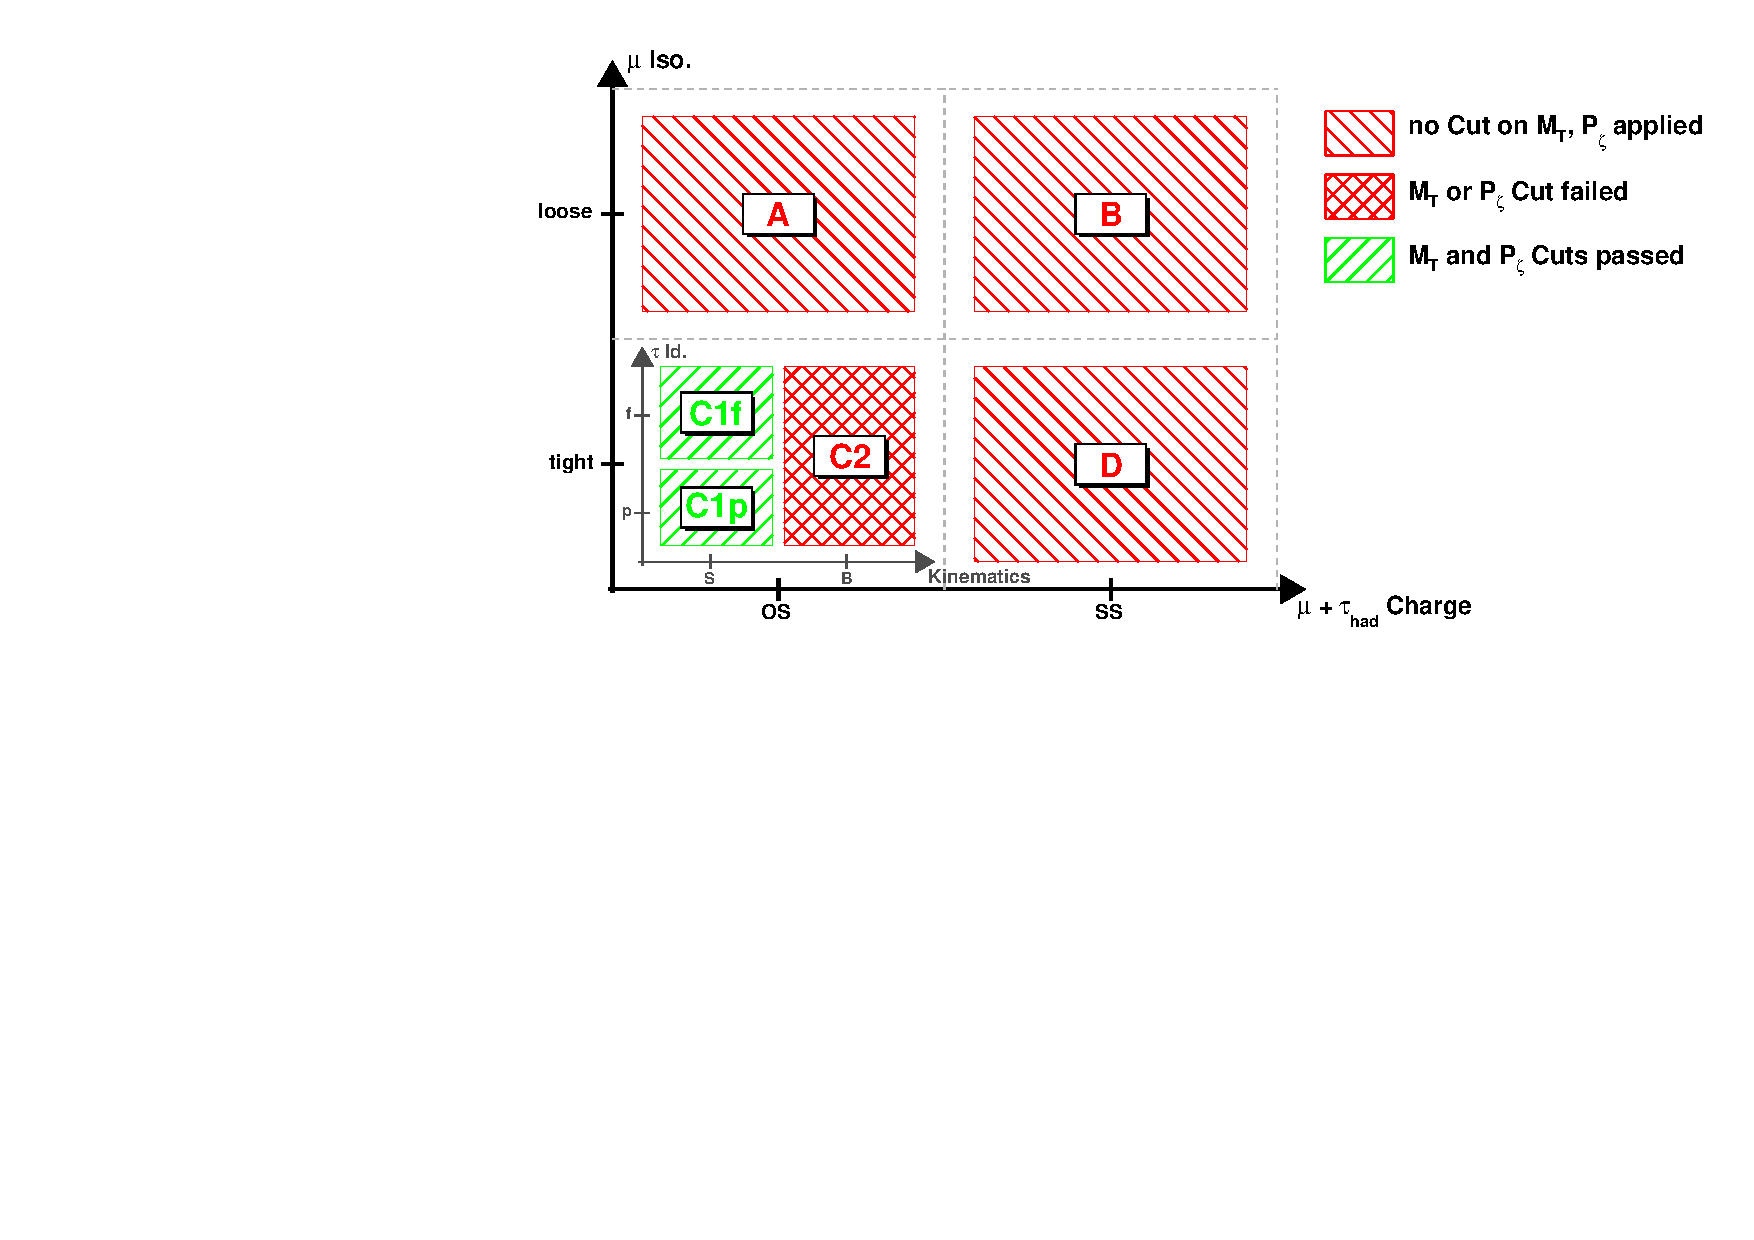
\includegraphics[angle=-0,width=0.8\textwidth]{3_Evt_Reconstruction/pics/figTauIdEffIllustration.pdf}
\caption{Illustration of signal and control regions used in the efficiency measurement and their requirements.
\label{fig:tau_eff_ABCD}
}
\end{center}
\end{figure}

The processes considered signal and background in the tau identification efficiency measurement %as contributing in the defined regions 
are: $\Z\To\tau\tau$, $\Z\To\mu\mu$, $\W\To\ell\nu+\rm{Jets}$, $t\anti{t}+\rm{Jets}$\ and QCD multijet production processes. All the kinematic distribution shapes used for this processes in the analysis are taken from MC simulation and normalized to the NLO predictions with the exception of the QCD shape in the C1p and C1f regions, where, to mitigate the lack of MC statistics, the shape is taken from the data distribution in the B region with the additional requirements of $M_T < 40$\ GeV and $\pz -1.5 \cdot \pz^{vis} > -20$. 

The yield of each process contributing to the measurement is expressed as a product of the total yield ($N^i$), the probability to pass (or fail) the muon isolation ($p_{\mu\,\rm{Iso}}^i$), the probability to pass (or fail) the leading track charge requirement ($p_{ch}^i$), the probability to pass (or fail) the topological cuts ($p_{topo}^i$) and the probability pass (or fail) the given tau-identification discriminator, $p_{\tau ID}^i$. The parameters listed above, initialized to their MC expectation, are inferred from data with a simultaneous template fit of all the regions and the different signal and background components. The physical observables used for the template fit is the invariant mass of the visible decay products, also called \emph{visible mass}, ($M_{vis}$), for the C1p and C1f categories and the transverse mass of the muon and \MET for the others. Figure \ref{fig:TauID_2011_fits} shows the results of the template fit for the loose discriminator.

\begin{figure}
	\setlength{\unitlength}{1mm}
	\begin{center}
		\begin{picture}(150,170)(0,0)
			\put(0.5, 118){\mbox{\includegraphics*[height=52mm]{3_Evt_Reconstruction/pics/controlPlotsTauIdEff_wConstraints_A_diTauMt_tauDiscrHPScombLooseDBcorr_all_fitted_diTauVisMass_ewkBgSum.pdf}}}
			\put(78.0, 118){\mbox{\includegraphics*[height=52mm]{3_Evt_Reconstruction/pics/controlPlotsTauIdEff_wConstraints_B_diTauMt_tauDiscrHPScombLooseDBcorr_all_fitted_diTauVisMass_ewkBgSum.pdf}}}
			\put(0.5, 60){\mbox{\includegraphics*[height=52mm]{3_Evt_Reconstruction/pics/controlPlotsTauIdEff_wConstraints_C1p_diTauVisMass_tauDiscrHPScombLooseDBcorr_passed_fitted_diTauVisMass_ewkBgSum.pdf}}}
			\put(78.0, 60){\mbox{\includegraphics*[height=52mm]{3_Evt_Reconstruction/pics/controlPlotsTauIdEff_wConstraints_C1f_diTauVisMass_tauDiscrHPScombLooseDBcorr_failed_fitted_diTauVisMass_ewkBgSum.pdf}}}
			\put(0.5, 2){\mbox{\includegraphics*[height=52mm]{3_Evt_Reconstruction/pics/controlPlotsTauIdEff_wConstraints_C2_diTauMt_tauDiscrHPScombLooseDBcorr_all_fitted_diTauVisMass_ewkBgSum.pdf}}}
			\put(78.0, 2){\mbox{\includegraphics*[height=52mm]{3_Evt_Reconstruction/pics/controlPlotsTauIdEff_wConstraints_D_diTauMt_tauDiscrHPScombLooseDBcorr_all_fitted_diTauVisMass_ewkBgSum.pdf}}}
			\put(-5.5, 170.5){\small (A)}
			\put(72.0, 170.5){\small (B)}
			\put(-5.5, 112.5){\small (C1p)}
			\put(72.0, 112.5){\small (C1f)}
			\put(-5.5, 54.5){\small (C2)}
			\put(72.0, 54.5){\small (D)}
		\end{picture}
		\caption{
         Measured distributions of $M_{T}$\ for the regions $A$, $B$, $C2$\ and $D$\ and of $M_{vis}$\ for $C1p$\ and $C1f$\ compared to the sum of templates associated to the signal and background processes. ``EWK Bgr.'' denotes the sum of $Z \to \mu^{+} \mu^{-}$\ and $W$\ + jet background contributions. The templates are scaled by normalization factors obtained by the fit for the loose working-point of the HPS combined isolation discriminator.
}
		\label{fig:TauID_2011_fits}
	\end{center}
\end{figure}


The inferred probability to pass the tau identification discriminator is related to its efficiency by:

\begin{equation}
 \epsilon_{\tau ID} = p_{\tau ID} \cdot \epsilon_f \cdot \epsilon_p \cdot \epsilon_i \cdot k_{jet \To \tau} \cdot k_p \cdot k_i
\end{equation}

Where the symbols $\epsilon$\ denote the preselection efficiencies and $k$\ the correction factors. The correction factors account for the fraction of taus that would pass the tau identification, but fail either the jet isolation ($k_i$), or the leading track requirement ($k_p$), and for the small amount of quark and gluon jets present in the $\Z\To\tau\tau$\ templates ($k_{jet \To \tau}$). These correction factors are extracted from MC simulation. 

The measured hadronic tau identification efficiency is compared to the MC prediction. %computed as a deviation from the predicted efficiency of the MC simulation. 
The efficiencies measured for all the tau identification discriminators are found to be in agreement with the MC prediction within the uncertainties, even though a small trend towards lower values may be seen for the tighter working points. The uncertainty in the efficiency for hadronic tau decays to pass the working point used in the search for the $\rm{H}\To\tau\tau$ presented in this thesis amounts to 
 6\% with an identification efficiency of roughly 60\%. The uncertainty represents the sum of statistical and systematic uncertainties added in quadrature. The main source of statistical error comes from the large uncertainties in the $\Z\To\tau\tau$ yield in the C1f region, while the leading systematic uncertainty is the reconstruction efficiency for hadronic tracks. A summary of the systematic uncertainties considered in the measurement can be found in Table~\ref{tab:tau_eff_sys}.

\begin{table}
\begin{center}
\caption{Summary of systematic uncertainties considered in the hadronic tau identification efficiency measurement, and their effect on the final result.}
\label{tab:tau_eff_sys}
\begin{tabular}{|c|c|}
 \hline
 systematic uncertainty & effect \\
 \hline
Muon momentum scale & $\ll 1\%$ \\
$\tau$--Jet energy scale & $ < 1\%$ \\
Hadronic track reconstruction & $3.9\%$ \\
Track momentum scale & $< 1\%$ \\
Loose Isolation & $2.5\%$ \\
$\rm{Jet}\To\tau_h$ fake rate & $1.2\%$ \\
$k_p$ uncertainty & $1.7\%$ \\
$k_i$ uncertainty & $2.1\%$ \\
Statistical uncertainty & $2.6\%$ \\
\hline
Total & $6.0\%$ \\
\hline
\end{tabular}
\end{center}
\end{table}


\subsubsection{Jet fake probability}

The $\rm{jet} \To \tau_h$ fake probability is measured using $\W+\rm{Jets}$ and QCD events. Events are selected online by a single--muon (W events) or single--jet (QCD events) trigger. W+Jets events are required to contain a well identified and isolated muon with $M_T(\mu, \met) > 50$ GeV. The $\rm{jet} \To \tau_h$ fake probability is computed for all taus with $\pt > 20$ GeV, $|\eta| < 2.3$ and passing the combination of ``decay mode finding'' plus the isolation discriminator under study with respect to all jets of $\pt > 20$ GeV and $|\eta| < 2.3$ \cite{DP-14-015}:

\begin{equation}
 p(jet \To \tau_h) = \dfrac{\operatorname{N}(\pt^{\tau_h} > 20\GeV \AND |\eta^{\tau_h}| < 2.3 \AND \mathrm{Decay-Mode} \AND \mathrm{Discriminator\,WP})}{\operatorname{N}(\pt^{jet} > 20\GeV \AND |\eta^{jet}| < 2.3)}
\end{equation}

The $jet \To \tau_h$ fake probability measured in W+jets events as a function of jet \pT, $\eta$, $\phi$ and as a function of the number of reconstructed vertices is shown in Figure \ref{fig:jetToTauFakeRate_Wjets_HPScombIso3Hit}. The $jet \To \tau_h$ fake probability is found to be strongly dependent to the jet \pT. An increase of the fake probability is also observed at high $\eta$ values, where the tracking efficiency decreases, affecting the discriminating power of the isolation-based discriminators. A mild dependence on the number of pileup vertices is also observed. This effect is due to the \db correction, which gradually switches off the neutral isolation discrimination as the pileup increases, leaving only the track-based isolation. Please note that the \db correction has been tuned to keep the efficiency constant as a function of the number of pileup interactions, causing the fake-rate to increase; another possible solution could have been keeping the fake-rate stable at the cost of reducing the efficiency. The slight mismatch between data and MC prediction is due to a mismodeling in the simulation of \emph{out-of-time pileup}, i.e. the effect that collisions from previous bunch crossings have in the current event. This effect is visible only in high-latency detectors such as the ECAL.

\begin{figure}
\setlength{\unitlength}{1mm}
\begin{center}
\begin{picture}(150,150)(0,0)
\put(-2.5, 74.5){\mbox{\includegraphics*[height=74mm]{3_Evt_Reconstruction/pics/jetToTauFakeRateVsPt_Wjets_HPScombIso3Hit.pdf}}}
\put(80.0, 74.5){\mbox{\includegraphics*[height=74mm]{3_Evt_Reconstruction/pics/jetToTauFakeRateVsEta_Wjets_HPScombIso3Hit.pdf}}}
\put(-2.5, -1.5){\mbox{\includegraphics*[height=74mm]{3_Evt_Reconstruction/pics/jetToTauFakeRateVsPhi_Wjets_HPScombIso3Hit.pdf}}}
\put(80.0, -1.5){\mbox{\includegraphics*[height=74mm]{3_Evt_Reconstruction/pics/jetToTauFakeRateVsNvtx_Wjets_HPScombIso3Hit.pdf}}}
\put(-5.5, 148.5){\small (a)}
\put(77.0, 148.5){\small (b)}
\put(-5.5, 72.5){\small (c)}
\put(77.0, 72.5){\small (d)}
\end{picture}
\end{center}
\caption{
  Probabilities for quark and gluon jets in $W$+jets events to pass the \emph{HPS combined isolation 3--hit}) discriminator, as function of jet $P_{T}$ (a), $\eta$ (b), $\phi$ (c) and as function of $N_{vtx}$, the number of vertices reconstructed in an event (d). The probabilities measured in data are compared to the Monte Carlo expectation.}
\label{fig:jetToTauFakeRate_Wjets_HPScombIso3Hit}
\end{figure}


\subsubsection{Electron and Muon fake probability}

The rejection power of the anti-electron and anti-muon discriminators is computed in $\Z\To\ell\ell$ events with a tag-and-probe technique. Well identified and isolated leptons are used to select the events both online and offline. The event is required also to contain a tau candidate passing only the decay-mode finding plus loose isolation discriminators (probe). The dimuon invariant mass distribution is fitted both in regions passing and failing the anti-lepton requirement to extract the rejection power and the ratio between data and MC. 

%The achieved rejection power for the two leptons is summarized in Table \ref{tab:tau_lep_rej}

%\begin{table}
%\begin{center}
%\caption{TODO, put values!}
%\begin{tabular}{|c|c|c|}
% \toprule
% Working point & efficiency & rejection power \\
% \midrule
% \multicolumn{3}{|c|}{muon rejection} \\
% \hline
% Loose & XX\% & XX\% \\
% Tight   & XX\% & XX\% \\
% \hline
% \multicolumn{3}{|c|}{electron rejection} \\
% \hline
% Loose    & XX\% & XX\% \\
% Medium & XX\% & XX\% \\
% Tight     & XX\% & XX\% \\
% Very Tight & XX\% & XX\% \\
% \bottomrule
%\end{tabular}
%\end{center}
%\label{tab:tau_lep_rej}
%\end{table}

\chapter[$pp\rightarrow\W\rm{H}$]{Search for the Higgs boson in tau decays in the process $pp\rightarrow\W\rm{H}$}%Search for a Standard Model Higgs boson in association with a W}

As described in Chapter 1, the Higgs boson is produced at the LHC via three main processes: the gluon fusion (GF), the vector boson fusion (VBF) and the associated production (VH). The VH process has a production cross section one order of magnitude smaller than the dominant gluon fusion process. The presence of an additional high-\pT lepton enhances the signal over background ratio significantly,  increasing the sensitivity of the VH channel to a level that is comparable to the sensitivity of the GF process. 
%Moreover, the associated production is a promising channel to measure the tau Yukawa coupling once enough integrated luminosity will be collected. \bold{ TODO: I STILL HAVE TO EXPLAIN WHY}

In this chapter we describe the search for the associated production of a W and a Higgs boson, where the W boson decays into a light lepton (electron or muon, generically denoted as $\ell$ from now on) and a neutrino, and the Higgs boson decays into a tau pair, with one tau decaying leptonically and the other tau hadronically. Three final states are considered: $\mu\mu\tau_h$, $e\mu\tau_h$ and $ee\tau_h$. 

\section{Event Selection}

Events are selected in real time by the double lepton triggers, which require the presence of either two muons, two electrons or a muon plus an electron. Evolving running conditions and increasing instantaneous luminosity imposed a tuning of the trigger object requirements in order to meet the constraints in trigger bandwidth. %Trigger paths, i.e. the ensemble of the selections for a certain type of trigger, having a excessive acceptance rate have been suppressed by randomly sampling them (a procedure called \emph{prescale}).

The unprescaled triggers with the lowest \pT thresholds available for each running period have been chosen. This choice results in \pT thresholds ranging from 7 up to 17~GeV and from 7 to 8 GeV for the leading and sub-leading muons in the double muon trigger. The \pT thresholds of the muon plus electron and of the double electron triggers have been kept constant at 17 GeV for the leading object and 8 GeV for the sub-leading lepton. The electron isolation criteria have been tightened as instantaneous luminosity increased. %but electrons underwent a progressively tighter selection according to their isolation value. 
A more detailed description of the electron and muon triggers can be found in~\cite{Chatrchyan:2012xi,CMS-PAS-EGM-10-004}.

In the offline event selection, leptons are selected according two sets of criteria called ``loose'' and ``tight''. %The distinction between loose and tight leptons is used to model the irreducible background as will be described in the following sections. 
Tight lepton requirements are applied when selecting signal events. The loose lepton selection, which is a subset of the tight one, is used to enhance the event statistics for the purpose of modeling the backgrounds as described in the following sections.

\begin{itemize}
\item Loose muons are required to:
\begin{itemize}
\item be reconstructed as global or tracker muons;
\item have $\pt > 10$ GeV, $|\eta| < 2.4$, $|d_Z| < 0.2$ cm;
\item have at least one hit in the pixel detector, to discriminate against in-flight decays;
\item the jet nearest to the muon in \DR is required not to pass the loose $b$-tagging discriminator. This cut is applied to reject $t\anti{t}$ events.
\end{itemize}

\item Loose electrons are required to:
\begin{itemize}
\item have $\pt > 10$ GeV, $|\eta| < 2.5$, $|d_Z| < 0.2$ cm;
\item have no missing tracker hits; 
\item have ``tight'' charge agreement, i.e. the curvature of the CTF, the GSF and the pixel-only tracks should agree. This requirement reduces the electron charge mis-identification;
\item the jet closest to the electron is required not to pass the loose $b$-tagging discriminator, to reject $t\anti{t}$ events
\end{itemize}

\item Loose taus are required to:
\begin{itemize}
\item have $\pt > 20$ GeV, $|\eta| < 2.3$, $|d_Z| < 0.2$ cm;
\item pass the ``decay-mode finding'' discriminator as described in Section~\ref{sec:tau_id}; 
\item not overlap with any electron passing loose MVA identification criteria plus isolation $Iso_{rel} < 0.3$, computed with \db correction applied in a cone of radius $\Delta R < 0.4$.
\end{itemize}

\end{itemize}

The offline event selection is different for the three channels and is detailed in the following sections:

\subsubsection{$\boldsymbol{\mu\mu\tau_h}$}
\begin{itemize}
\item The event must pass the lowest-threshold unprescaled double muon trigger;
\item Both muons must be matched to the corresponding trigger candidates;
\item The leading muon must have $\pt > 20$ GeV, to be compliant with the online thresholds;
\item Both muons must pass the PF Tight identification working point;
\item The $\Delta \beta$-corrected relative PF isolation of the leading muon, computed in a cone of $\Delta R < 0.4$ has to be less than 0.15 (0.1) for muons with $|\eta| < 1.479$ ($|\eta| > 1.479$);
\item The $\Delta \beta$-corrected relative PF isolation of the sub-leading muon, computed in a cone of $\Delta R < 0.4$ has to be less than 0.2 (0.15) for muons with $|\eta| < 1.479$ ($|\eta| > 1.479$);
\item The hadronic tau candidate is required to pass the loose HPS combined isolation working point to suppress the backgrounds with jets misidentified as $\tau_h$, the loose electron rejection working point plus the tight muon rejection working point. The latter is applied to suppress the background process $\Z\To\mu\mu+\rm{jet}$ where a muon is misidentified as the hadronic tau and the jet as a muon.
\end{itemize}

\subsubsection{$\boldsymbol{e\mu\tau_h}$}
\begin{itemize}
\item The event must pass the lowest-threshold unprescaled muon plus electron trigger, which imposes a 17 GeV threshold on the leading lepton \pT and a 8 GeV threshold on the sub-leading one, independently on the flavor of the light leptons;
\item Both the electron and the muon must be matched to the corresponding trigger candidates;
\item The muon is required to have $\pt > 20$ GeV if the trigger accepting the event has a 17 GeV threshold on the muon candidate;
\item The electron is required to have $\pt > 20$ GeV if the trigger accepting the event has a 17 GeV threshold on the electron candidate;
\item The electron is required to pass the ``loose'' MVA identification working point;
\item The electron $\Delta \beta$-corrected relative PF isolation in a cone of $\Delta R < 0.4$ has to be less than 0.15 (0.1) for candidates with $|\eta| < 1.479$ ($|\eta| > 1.479$);
\item The muon $\Delta \beta$-corrected relative PF isolation in a cone of $\Delta R < 0.4$ has to be less than 0.15 (0.1) for candidates with $|\eta| < 1.479$ ($|\eta| > 1.479$);
\item The hadronic tau candidate is required to pass the loose HPS combined isolation working point to suppress the backgrounds with jets misidentified as $\tau_h$.
\item To suppress $\Z\To e^\pm e^\mp+\rm{jet}$ background with an electron misidentified as the hadronic tau and a jet as the muon, events with $|M_{e\tau} - M_\Z| < 20\GeV$, where $M_{e\tau}$ is the invariant mass of the electron and the hadronic tau and $M_\Z = 91.2$ GeV, i.e. the mass of the Z boson, are required to contain a tau passing the medium electron rejection working point, otherwise the tau is required to pass the loose one;
\item To suppress $\Z\To\mu^\pm \mu^\mp+\rm{jet}$ background with a muon misidentified as the hadronic tau and a jet as the electron, events with $|M_{\mu\tau} - M_\Z| < 20\GeV$, where $M_{\mu\tau}$ is the invariant mass of the muon and the hadronic tau, are required to contain a tau passing the tight muon rejection working point, otherwise the tau is required to pass the loose one;
\end{itemize}

\subsubsection{$\boldsymbol{ee\tau_h}$}
\begin{itemize}
\item The event must pass the lowest-threshold unprescaled double electron trigger; 
\item Both the electrons must be matched to the corresponding trigger candidates;
\item The leading electron must have $\pt > 20$ GeV, to be compliant with the online thresholds, and pass the tight MVA electron identification working point;
\item The $\Delta \beta$-corrected relative PF isolation of leading electron, computed in a cone of $\Delta R < 0.4$ is required to be less than 0.15 (0.1) for electrons with $|\eta| < 1.479$ ($|\eta| > 1.479$);
\item The sub-leading electron must pass the loose MVA electron identification working point and its $\Delta \beta$-corrected relative PF isolation in a cone of $\Delta R < 0.4$ is required to be less than 0.2 (0.15) for electrons with $|\eta| < 1.479$ ($|\eta| > 1.479$);
\item The hadronic tau is required to pass the loose HPS combined isolation working point, the loose electron rejection working point and the tight muon rejection working point;
\item To suppress $\Z\To e^\pm e^\mp+\rm{jet}$ background with an electron misidentified as the hadronic tau and a jet as electron, events with $|M_{e_{1,2}\tau} - M_\Z| < 10\GeV$, where $M_{e_{1,2}\tau}$ is the invariant mass of the hadronic tau and either electron, are required to contain a tau passing the tight electron rejection working point.                                                                         
\item In events with $10\GeV < |M_{e_{1,2}\tau} - M_Z| < 20\GeV$ the tau is required to pass the medium electron rejection working point.                                                               
\item This channel suffers from an additional source of background that is due to DY events in which the charge of either electron is mis-measured. %with one of the electrons being measured with the wrong charge. 
A detailed description of the studies conducted to model this background is presented in the following section of the note. In order to suppress this type of background events with $|M_{ee} - M_\Z| < 10$ are rejected.                                                                                                                                                                 
\end{itemize}

In all the channels the three leptons are required to be separated by a \DR distance of at least 0.4, in order to avoid that their isolation cones overlap.

In addition to the selection criteria given above, the electrons and muons in the events are required to be of the same charge. This requisite greatly suppresses the background contamination from $\Z/\gamma \to \ell^\pm \ell^\mp + \rm{jet}$ and $t\anti{t}$ in which a jet is misidentified as hadronic tau.

To reduce the contamination from ZZ and $t\anti{t}$ backgrounds, events with additional isolated electrons, muons, hadronic taus or $b$-tagged jets are rejected. None of these vetoes but the $b$-jet one
have a significant effect on the signal efficiency of the analysis. The b-jet veto was found to degrade the final expected limit by about 4\%, but is nevertheless included to avoid any overlap of the
signal region with searches in the $t\anti{t}H$ channel~\cite{CMS-PAS-HIG-13-019}.

The offline event selection has been optimized for each channel separately, maximizing the expected significance to discover a 125 GeV SM Higgs boson signal. To perform this maximization, the full background estimation procedure, detailed in the following sections, has been used with a simpler systematics set-up. Electron identification and lepton isolation have been optimized simultaneously, while the $\Z\To\ell\ell+\rm{jet}$ background rejection has been optimized separately. The electron charge mis-identification rejection has been optimized in a separate procedure, considering only the $ee\tau_h$ channel.

\section{Background estimation}
%Problem description
%\subsection{Reducible and irreducible backgrounds}

The main background processes can be divided into two types: reducible (or fake) and irreducible backgrounds. The former category includes all those processes in which at least one of the final state leptons is mis-identified. The main process contributing to this category is the associated production of W and jets, where two jets are mis-identified as a light lepton and a hadronic tau, respectively. Further relevant background contributions arise from QCD multi-jet, $t\anti{t}$ and Z+Jets production. The Z+Jets contamination in particular needs a more detailed discussion. As the two light leptons are required to the have same charge, only two configurations are possible: in the first case one of the leptons from the Z decay is mis-identified as a hadronic tau while a jet is mis-identified as light lepton; in the second case one of the leptons is mis-reconstructed with the wrong charge. This effect is only relevant for electrons and is discussed in Section~\ref{sec:charge_misid}. The irreducible background is composed only by the dominant WZ production, which has the same signature as the process under study, and the ZZ one, in case one of the light leptons fails to be reconstructed.

\subsection{Irreducible backgrounds}

The irreducible backgrounds are modeled by the Monte Carlo simulation. The hard scattering process amplitudes are generated by \madgraph~\cite{MG4}, a leading order (LO) matrix element generator. The decay of long-living particles originating from the parton scattering and the hadronization process of quarks and gluons is handled by \pythia\ \cite{pythia}. \pythia\ also adds additional jets to simulate the presence of the underlying event. This process, as well as the hadronization, is performed with the aid of empirical parton fragmentation functions. The tau decay, which was found to be imprecisely simulated by \pythia, is simulated by \textsc{Tauola}~\cite{tauola}, a dedicated library. 

The presence of pileup in MC events is simulated by adding simulated \emph{minimum bias} events to the generated ``hard'' process. The distribution of pileup events in the simulated sample is different, and generally generated with higher pileup, with respect to real running conditions. 
This mis-match was created on purpose to ensure good coverage of the pileup distribution even for running periods posterior to the MC creation.
% as a precaution against unexpected rise in the machine instantaneous luminosity, as most of the times the MC samples have been produced during data-taking periods. 
Simulated events are therefore reweighted according to the number of pileup events in the MC and the distribution of pileup events in data. This procedure, called \emph{pileup reweighting}, removes the differences induced by the mis-match in the pileup distribution. The distribution of pileup events in real data is computed based on the luminosity profile and the inelastic p--p scattering cross section~\cite{Antchev:2013paa}.
%inferred by the luminosity monitors.

Residual differences concerning the trigger selection, lepton identification and isolation are accounted for with dedicated analyses yielding a set of data to MC correction factors and corresponding uncertainty. When differing from unity, these scale factors are applied to simulated samples in the form of an event weight.
Finally, events yields are scaled according to the NLO theoretical cross-section prediction~\cite{MCFM}. 

Measured and simulated kinematic distributions are compared in dedicated control regions with $\Z\To\mu\mu,e\mu,ee$ decays, shown in Figure~\ref{fig:(dis)agreement}. %This comparison is shown in Section XX.

\begin{figure}
\centering
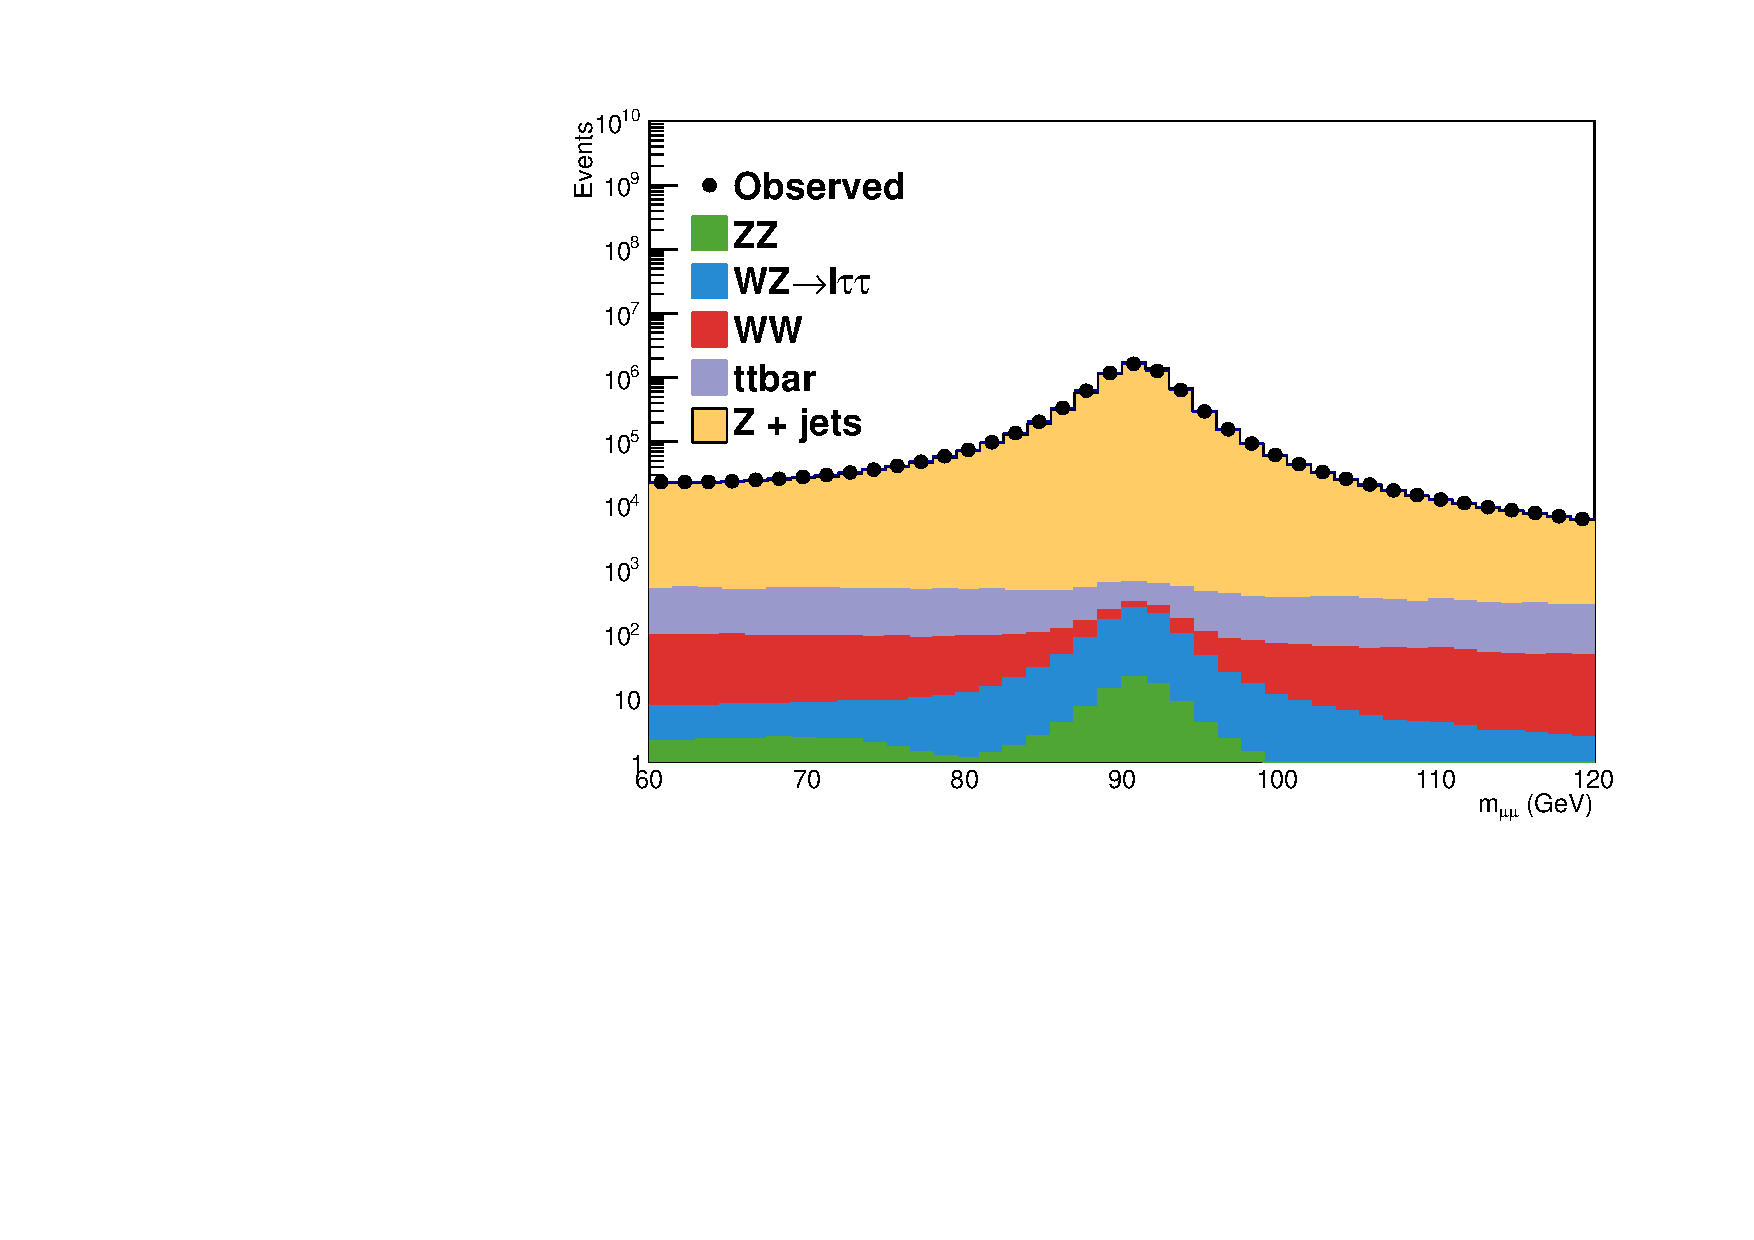
\includegraphics[width=0.49\textwidth]{4_Analisys/pics/8TeV/plots/zmm/mass_rebin_log.pdf}
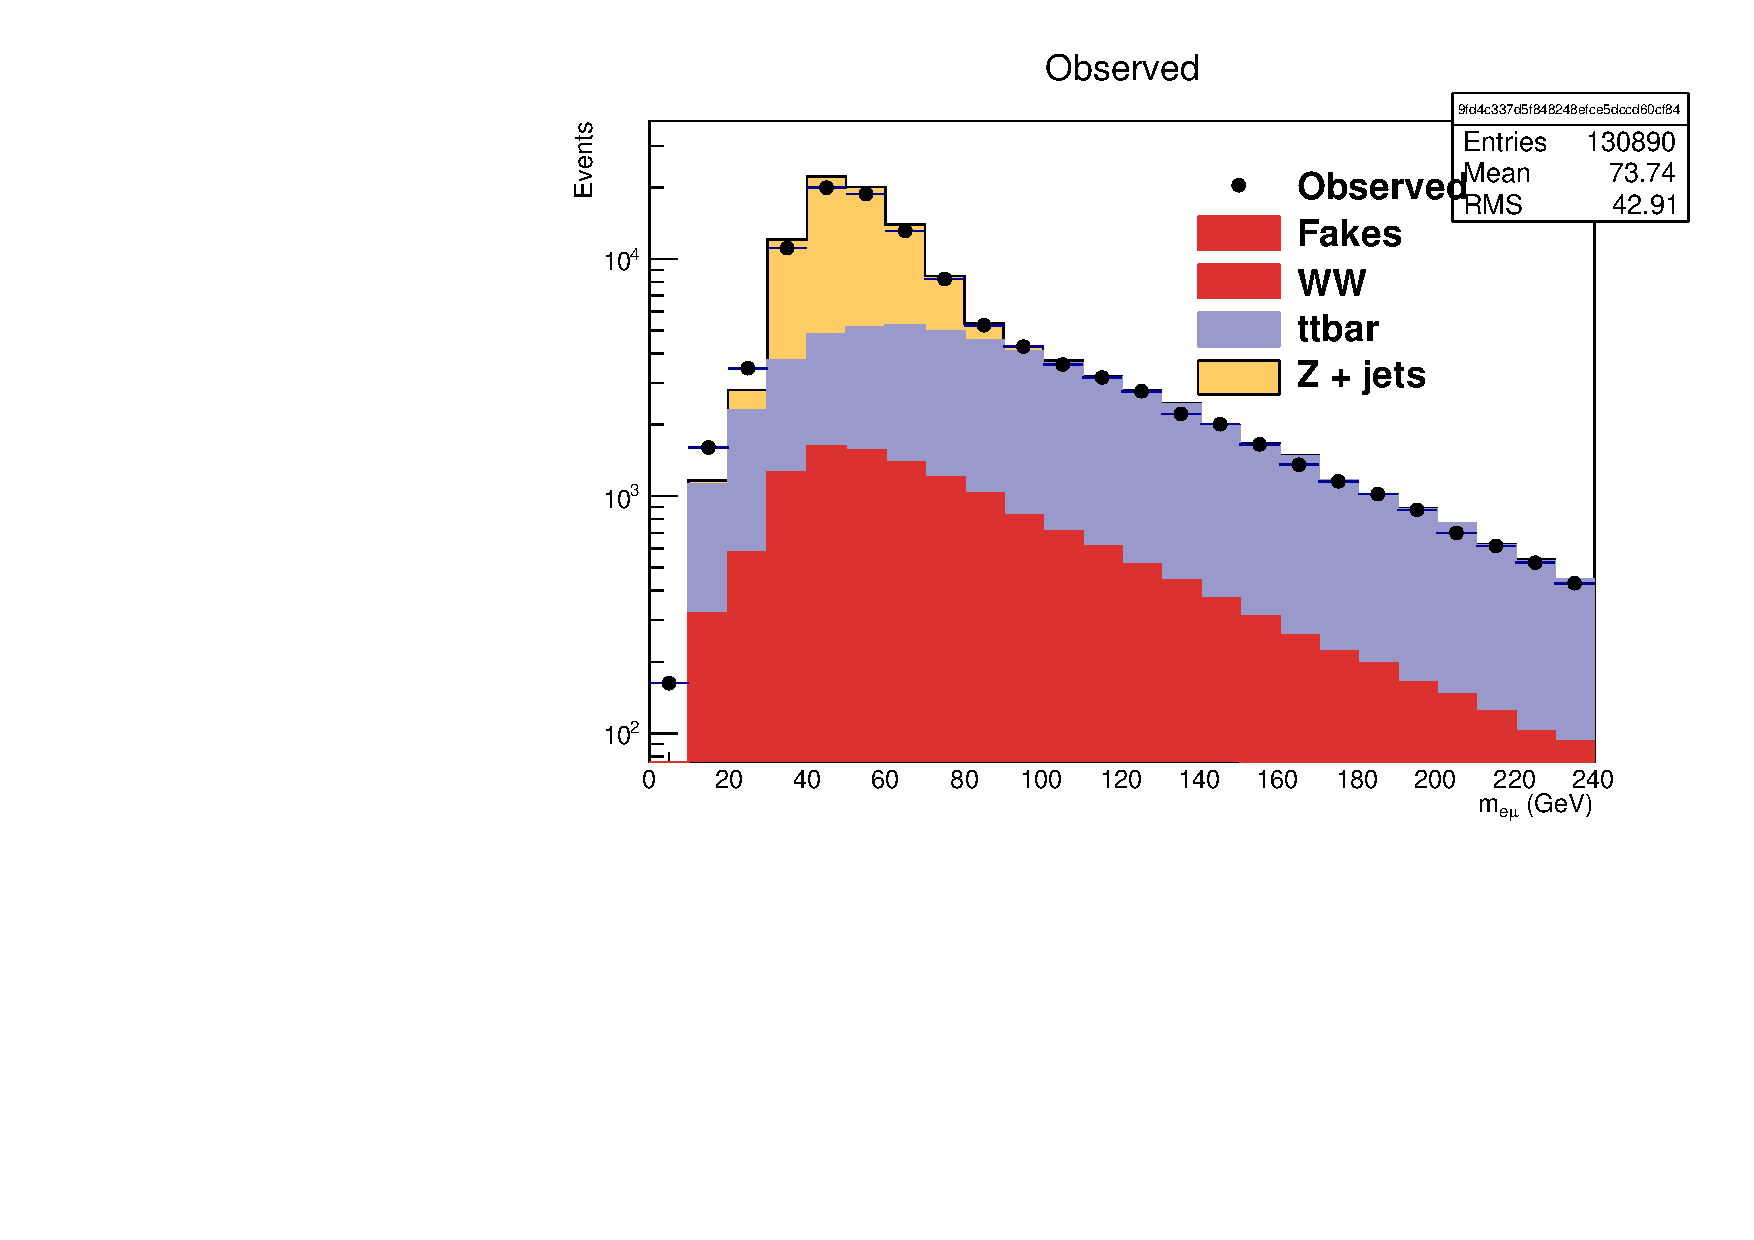
\includegraphics[width=0.49\textwidth]{4_Analisys/pics/8TeV/plots/em/mass_rebin_log-fakes.pdf}\\
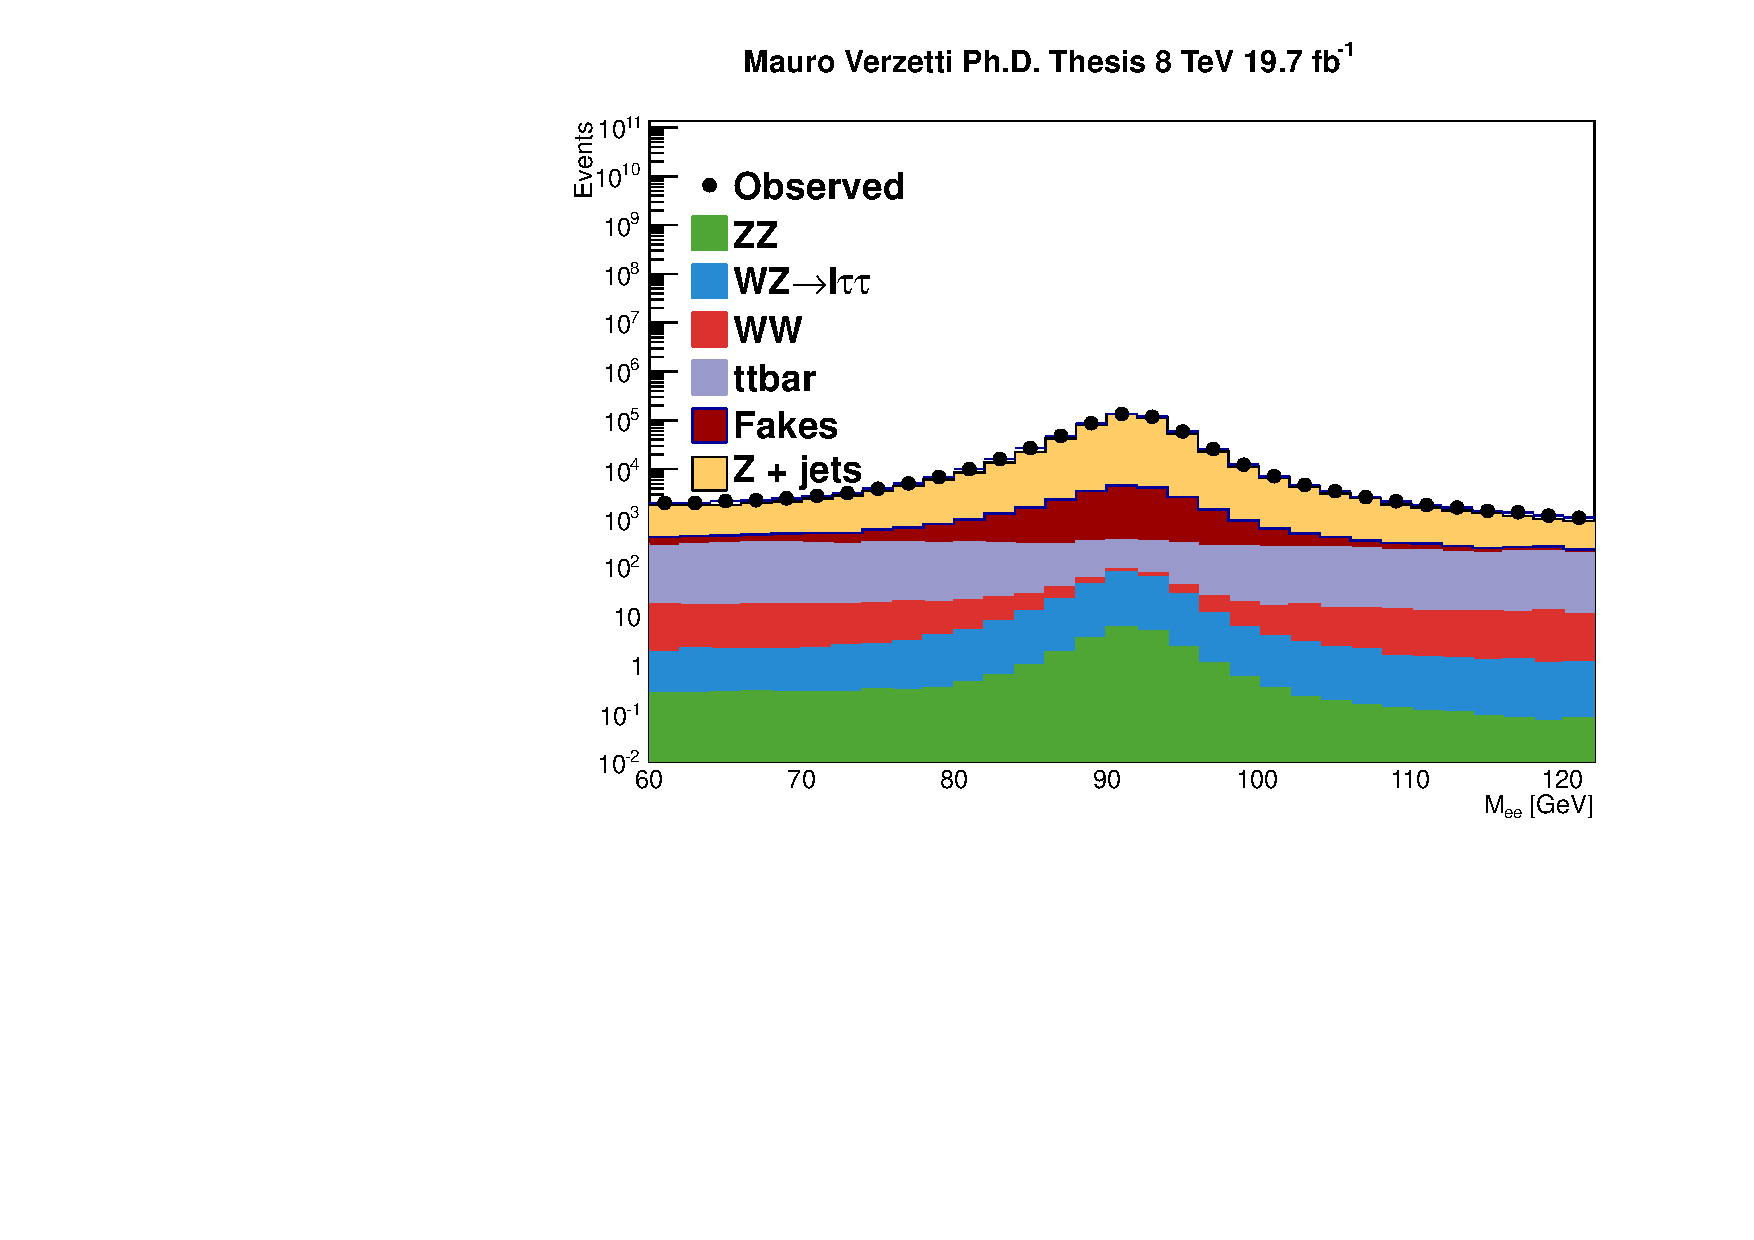
\includegraphics[width=0.49\textwidth]{4_Analisys/pics/8TeV/plots/zee/mass_wfakes_log.pdf}
\caption{Dilepton invariant mass distribution measured with 8 TeV data in dedicated $\Z\To\mu\mu$ (top left), $\Z\To \tau\tau \To e\mu$ (top right), and $\Z\To ee$ (bottom) control regions. Data are represented by solid points while the expectation is given by the stacked histogram. The background contributions labeled ``Fakes'' is estimated as described in Section~\ref{sec:fakemethod}. %are computed as the reducible background in the main analysis and described in the following section. 
}
\label{fig:(dis)agreement}
\end{figure}

\subsection{Reducible backgrounds}

The reducible background includes a wide range of processes with quark or gluon jets misidentified as leptons. %In these conditions a
A data-driven background estimation technique is preferred over simulation. %Due to these constraints 
In the work presented in this thesis the reducible backgrounds are estimated by means of the ``misidentification rate'' (or ``fake rate'') method.

The method consists of defining ``loose'' as well as ``tight'' selections for the lepton that can be faked by the jets, with the tight selection being the same as the final analysis selection used in this work.
The misidentification probability for a quark or gluon jet satisfying the loose lepton selections to pass the corresponding tight selection can be parametrized by a function $f(\vec{x})$ of a set of kinematic variables, $\vec{x}$, characterizing the event. This probability is measured in a dedicated control region resembling as closely as possible the signal region, while still being disjunct from it. The misidentification probability is then applied as weight to the events passing all selection criteria of the signal region except the tight lepton requirements. The weighted distributions obtained in this way represent the background contribution expected in the signal region.

%We study two possible background estimations: one using the $\rm{jet} \To \ell$ misidentification probability and the other using the $\rm{jet} \To \tau_h$ one. 
We compare the background estimates obtained by applying the method to the light leptons and to the tau leg. 
The former method is more inclusive as it accounts for all the sources of reducible backgrounds while the latter ignores those in which an isolated light lepton is mistakenly identified as a hadronic tau candidate. For these processes (i.e. Z+jets, WW, and part of $t\anti{t}$) the latter method relies on MC simulation. 

\subsection{Fake lepton method}
\label{sec:fakemethod}
\subsubsection{Control region definition}
The lepton misidentification probability is measured in a $W$+jets enriched control region.
This region differs from the signal one by requiring the transverse mass of the leading $\ell-\met$ system to exceed 55 GeV,
and vetoing events with more than two identified electron or muon candidates in the event. Events containing a well identified hadronic tau are vetoed as well, to remove any overlap with the signal region. In order to mimic the presence of a hadronic tau, the event is required to contain an additional jet with \pT above $20$ GeV.

Events selected in the control regions described above are used to train a k-Nearest Neighbor classifier (kNN)~\cite{TMVA}, which allows the parametrization of the misidentification probability as function of multiple variables. All the events selected in the control region are used to train the kNN.
Each parameter (dimension) is inversely scaled by its variance over the training sample, so that the (scaled) parameters are approximately normally distributed.
Leptons passing the tight lepton selection are marked as signal, those failing as background.
To find the misidentification probability at a particular point in the parameter space, the classifier searches for the $k$ nearest objects to the given point in the training sample.
The predicted efficiency is then the number of signal events among the $k$ neighbors and divided by $k$.

The input variable used for the training are the lepton \pT, the \pT of the jet associated to the lepton, and the number of jets with $\pt > 20$ GeV in the event. 
The first two variables, especially the jet \pT, are found to be strongly correlated to the probability for a jet to be mis-identified as a lepton. In particular, the difference of these two variables is linked to the isolation value of the lepton. In the training of the muon misidentification probabilities the logarithm of the jet \pT is used instead of the jet \pT to reduce the steep dependence of the probability with respect to this variable, allowing a larger number of neighbors to be used.
The number of jets was found to improve the description of the background shape. This variable is particularly effective in separating the different processes underlying the reducible background (W, multi-jet, and $t\anti{t}$). Another peculiarity of this variable is that it is bound to be $\geq 1$ in the training sample, while it can be zero in the main analysis. The difference is resolved by adding the number of hadronic taus in the event to the number of jets, resulting in a variable with the same range as the training variable.

The contribution of genuine isolated leptons from WZ and ZZ events in the control region is removed using simulated MC events and training dedicated kNN classifiers on them.
The output of the diboson kNN's is then scaled by:

\begin{equation}
\frac{N_{training}^{MC}}{N_{training}^{data}}\frac{\mathcal{L}^{data}}{\mathcal{L}_{eff}^{MC}}
\end{equation}

where $N_{training}^{i}$ is the number of events used for the training of either data or MC and $\mathcal{L}^{i}$ denotes the corresponding integrated luminosities. The output of the diboson kNN is finally subtracted to the output of the kNN trained on data.\footnote{Another equivalent option would have been to directly inject the simulated events in the training sample with negative weight proportional to the luminosity difference, but this method has been found to yield inconsistent results, most likely due to a wrong implementation in the TMVA framework.}

\subsubsection{kNN optimization and systematic uncertainties}
\label{sec:kNN_uncertainties}

The only adjustable parameter in the kNN training is the number of neighbors used to extract the probability. 
The optimal number of neighbors depends on the probability distribution of the different observables (more or less steeply varying) and on the statistics of the training sample. 
A large number of neighbors yields very accurate results, at the price of a reduced ability to describe abrupt changes in the probability function.

It is therefore important to define a procedure that determines the optimal number of neighbors to be used for each sample as function of the tight working point employed in the final analysis. This evaluation is performed with a bootstrapping technique.
Each training sample is initially split into two sub-samples, one containing 90\% of the events and the other the remaining 10\%. In order to remove any bias due to the run period (different pileup conditions) the smaller dataset is evenly sampled from the full dataset. This procedure is repeated ten times to obtain a set of mutually exclusive pairs of ``large'' and ``small'' samples. Subsequently, a training of the kNN classifier is performed on each large sample and applied to the small one. This procedure ensure a total decoupling between testing and training samples. The small size difference between the large sample and the full dataset also ensures that the results inferred from the major dataset are still statistically valid for the full one. The outcome of the ten training and testing cycles is then combined. 

The full process is repeated to scan over a wide range of values for the number of neighbors, $k$. A strong limiting factor for this method is the significant computing resource usage, as the computing complexity of training and testing of the kNN algorithm is proportional to the number of neighbors used.% The choice of the tested points and their maximum value are a direct consequence of this limitation: as the number of neighbors increases, the scan becomes more coarse.

For each choice of k, the shape of important physics observables is computed based on the weighted sum of all the events in the small samples and from the passing events. The two shapes are compared using as figure of merit the $\chi^2$ compatibility between the two shapes. The physical observable used for the $\chi^2$ minimization is the scalar sum of the \pT of the two leptons plus the jet, similar to the $L_T$ variable used further on in the analysis. Other variables were also considered and found to yield similar conclusions concerning the optimal choice of $k$.%compatible results. 

The minimum $\chi^2$ value obtained by the scan is taken to define $k$ for training the final kNN algorithm used in the analysis. %as reference value of number of neighbors to be used for training in the analysis. 
A parabolic fit around the minimum is performed to estimate the one sigma confidence interval as the value for which the parabolic fit yields the value of $\chi^2_{min} + 1$. %is $fcn(i) = \chi^2_{min} + 1$. 
This confidence interval reflects both the statistical uncertainties on the training sample and the related uncertainty on the choice of the training parameters. For each channel and each lepton, three classifiers are trained with the corresponding central values and one sigma boundaries.

A summary of the chosen minima and of the confidence interval boundaries is given in table~\ref{tab:kNN_minima}. A graphic representation of a sample scan is shown in figure~\ref{fig:kNN_minima_sample}. The misidentification rate observed in the training sample is displayed in figure~\ref{fig:fake_rate_sample}, overlaid with the output of the respective kNN classifier.


\begin{table}

\caption{Minimization points for each kNN scan and relative uncertainties as obtained from a parabolic fit}

\centering
\begin{tabular}{|c|c|c|c|c|}
\hline
channel & lepton & $-1\,\sigma$ & central value & $1\,\sigma$ \\
\hline
\multicolumn{5}{|c|}{7 TeV} \\
\hline
\multirow{2}{*}{ $\mu\mu\tau_h$ }& leading muon & 15 & 20 & 60\\
& sub-leading muon & 11 & 20 & 49\\
\hline
\multirow{2}{*}{ $e\mu\tau_h$ }& muon & 7 & 20 & 30\\
& electron & 634 & 1000 & 1807\\
\hline
\multirow{2}{*}{ $ee\tau_h$ }& leading electron & 35 & 200 & 686\\
& sub-leading electron & 381 & 1200 & 1723\\
\hline
\multicolumn{5}{|c|}{8 TeV} \\
\hline
\multirow{2}{*}{ $\mu\mu\tau_h$ }& leading muon & 28 & 40 & 73\\
& sub-leading muon & 30 & 40 & 63\\
\hline
\multirow{2}{*}{ $e\mu\tau_h$ }& muon & 16 & 20 & 30\\
& electron & 664 & 1400 & 2136\\
\hline
\multirow{2}{*}{ $ee\tau_h$ }& leading electron & 218 & 400 & 552\\
& sub-leading electron & 605 & 1000 & 2201\\
\hline
\end{tabular}

\label{tab:kNN_minima}
\end{table}

\begin{figure}
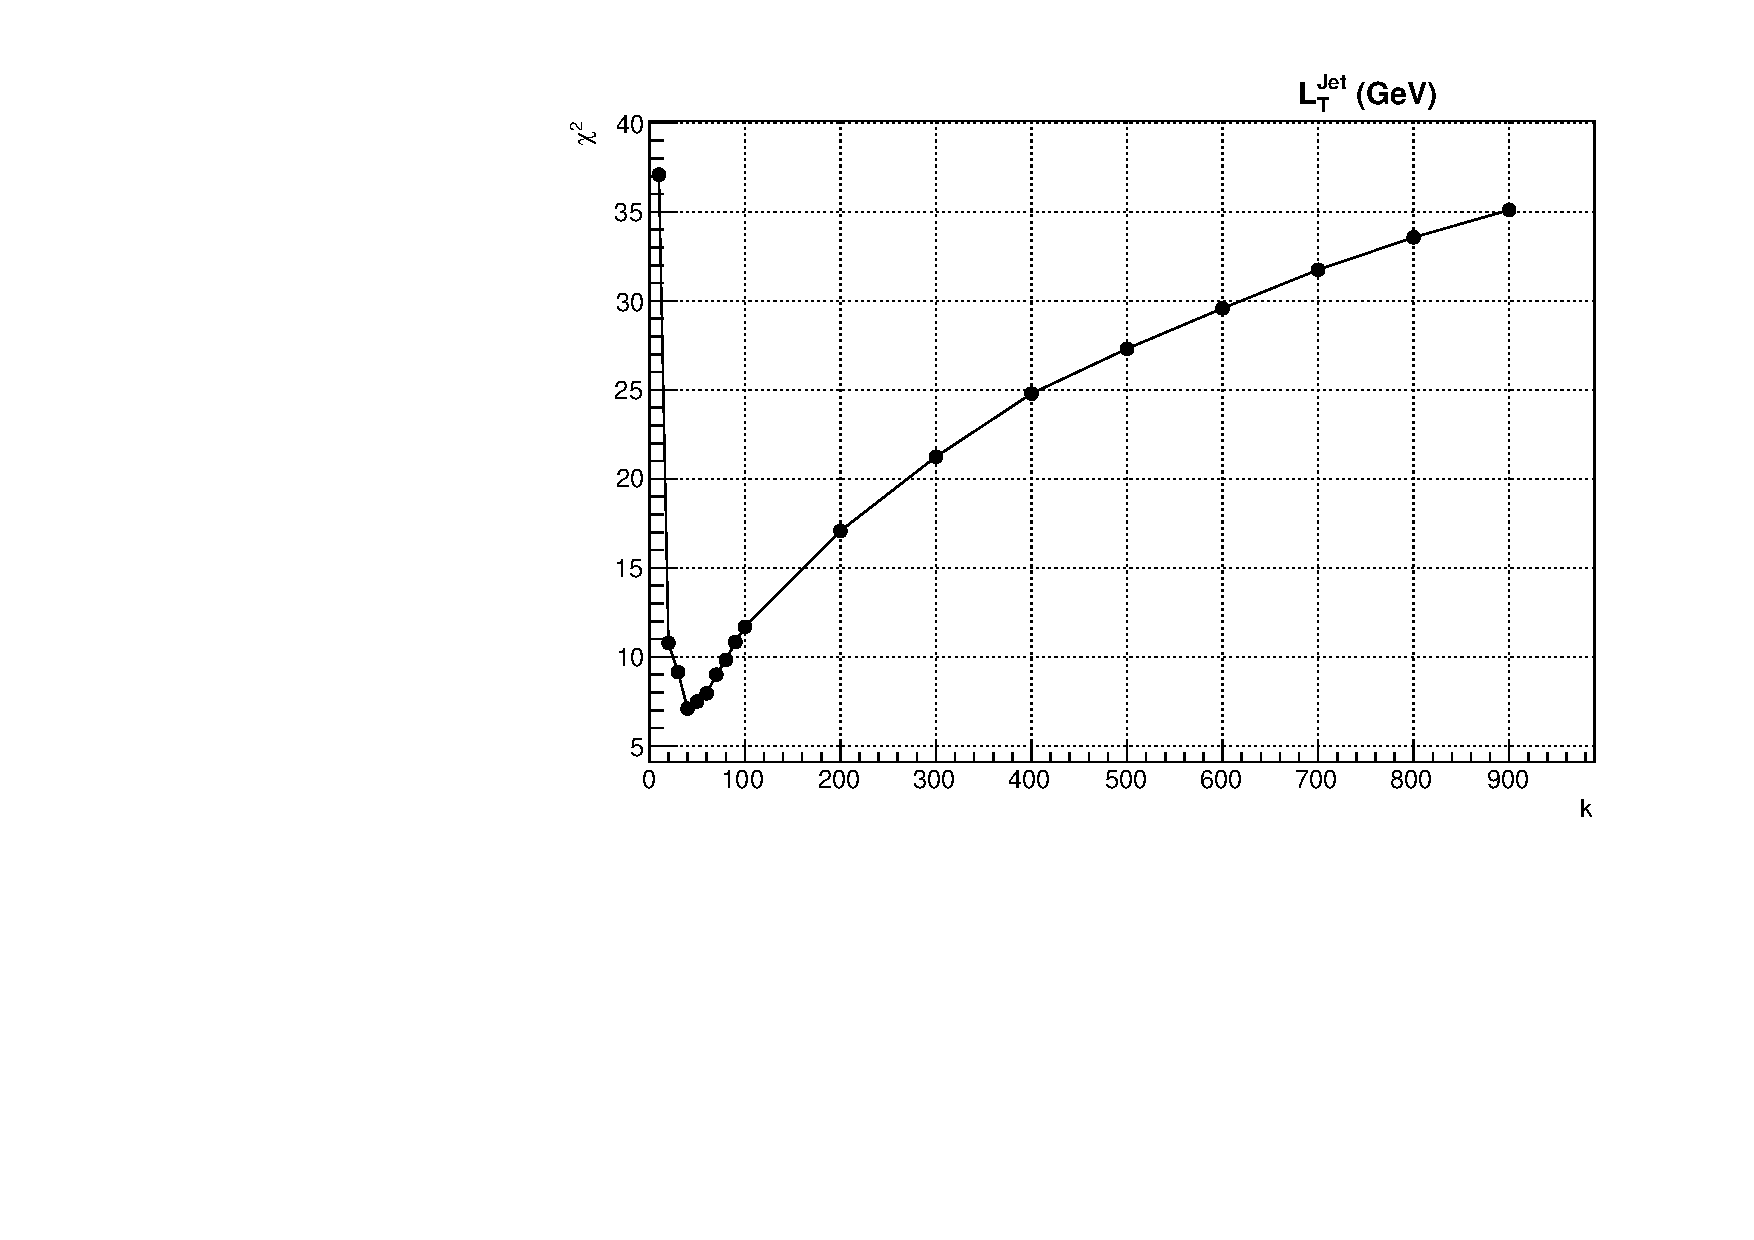
\includegraphics[width=0.5\textwidth]{4_Analisys/pics/8TeV/ProfileNeighbors/MM/h2taucuts020/LT_chi2.pdf}
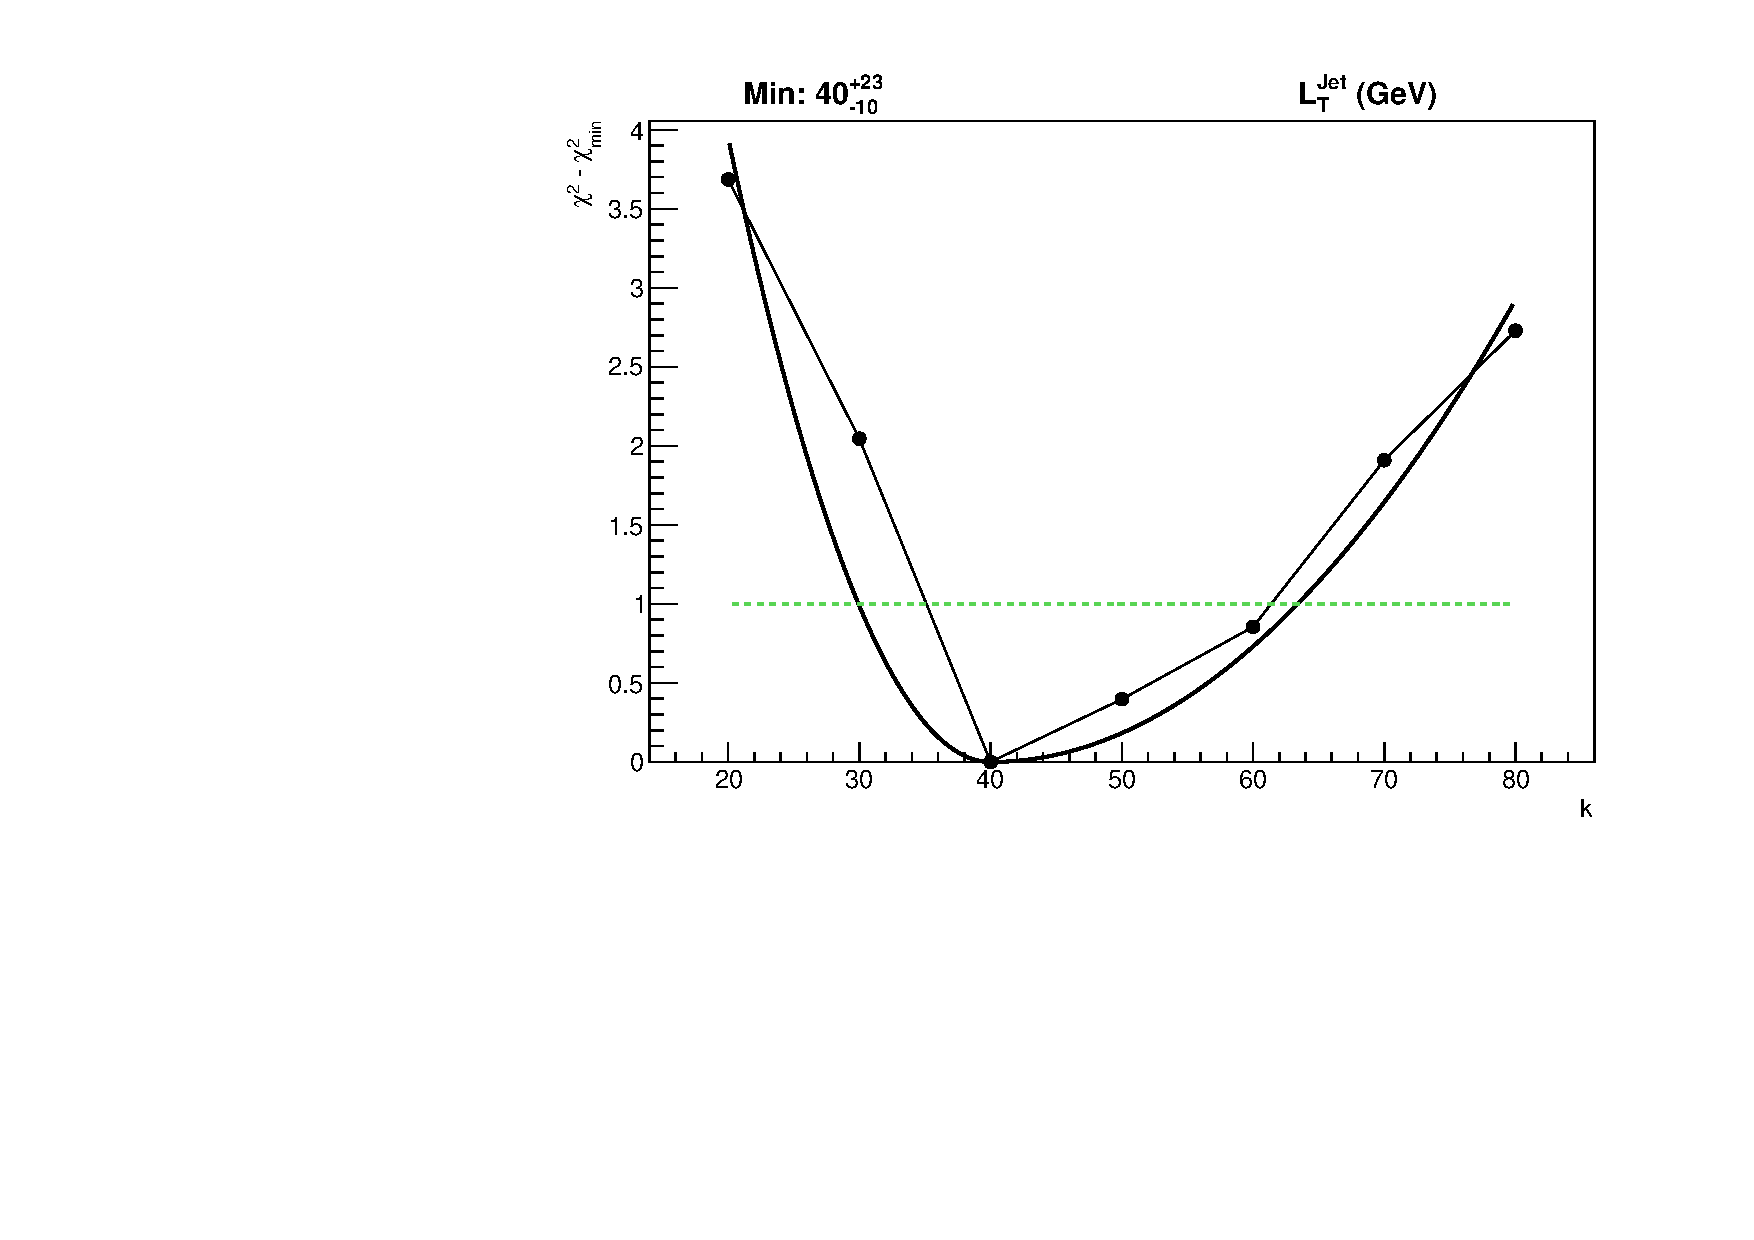
\includegraphics[width=0.5\textwidth]{4_Analisys/pics/8TeV/ProfileNeighbors/MM/h2taucuts020_LT.pdf} \\
\caption{\chisq as a function of the number of neighbors used in the kNN algorithm for background estimation 
(left) and corresponding fit (right) for sub-leading muons in the $\mu\mu\tau_h$ channel. The variable used for the scan is the scalar sum of the \pT of the two leptons and the jet}
\label{fig:kNN_minima_sample}
\end{figure}

\begin{figure}
\centering
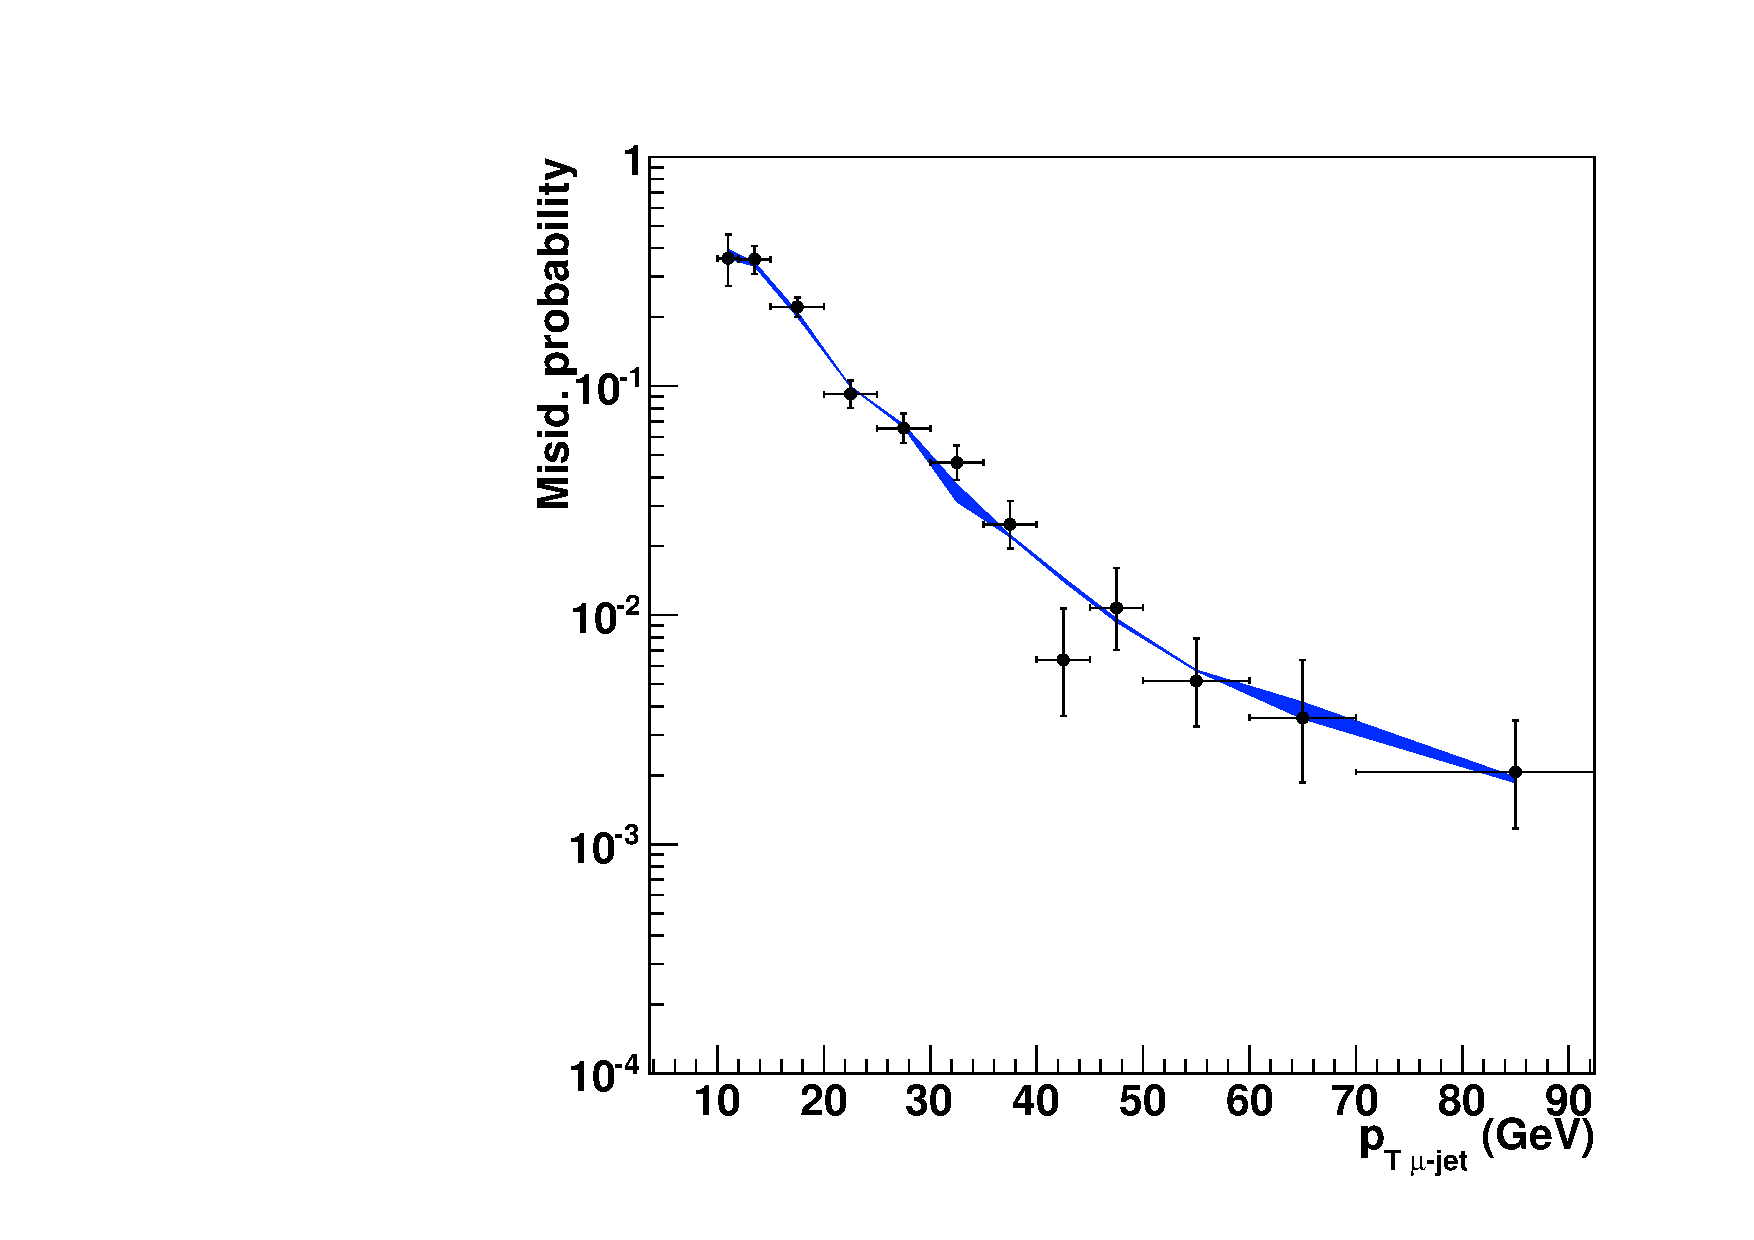
\includegraphics[width=0.49\textwidth]{4_Analisys/pics/8TeV/plots/fakerates/m_mmt_subleading_kNN_muonJetPt.pdf}
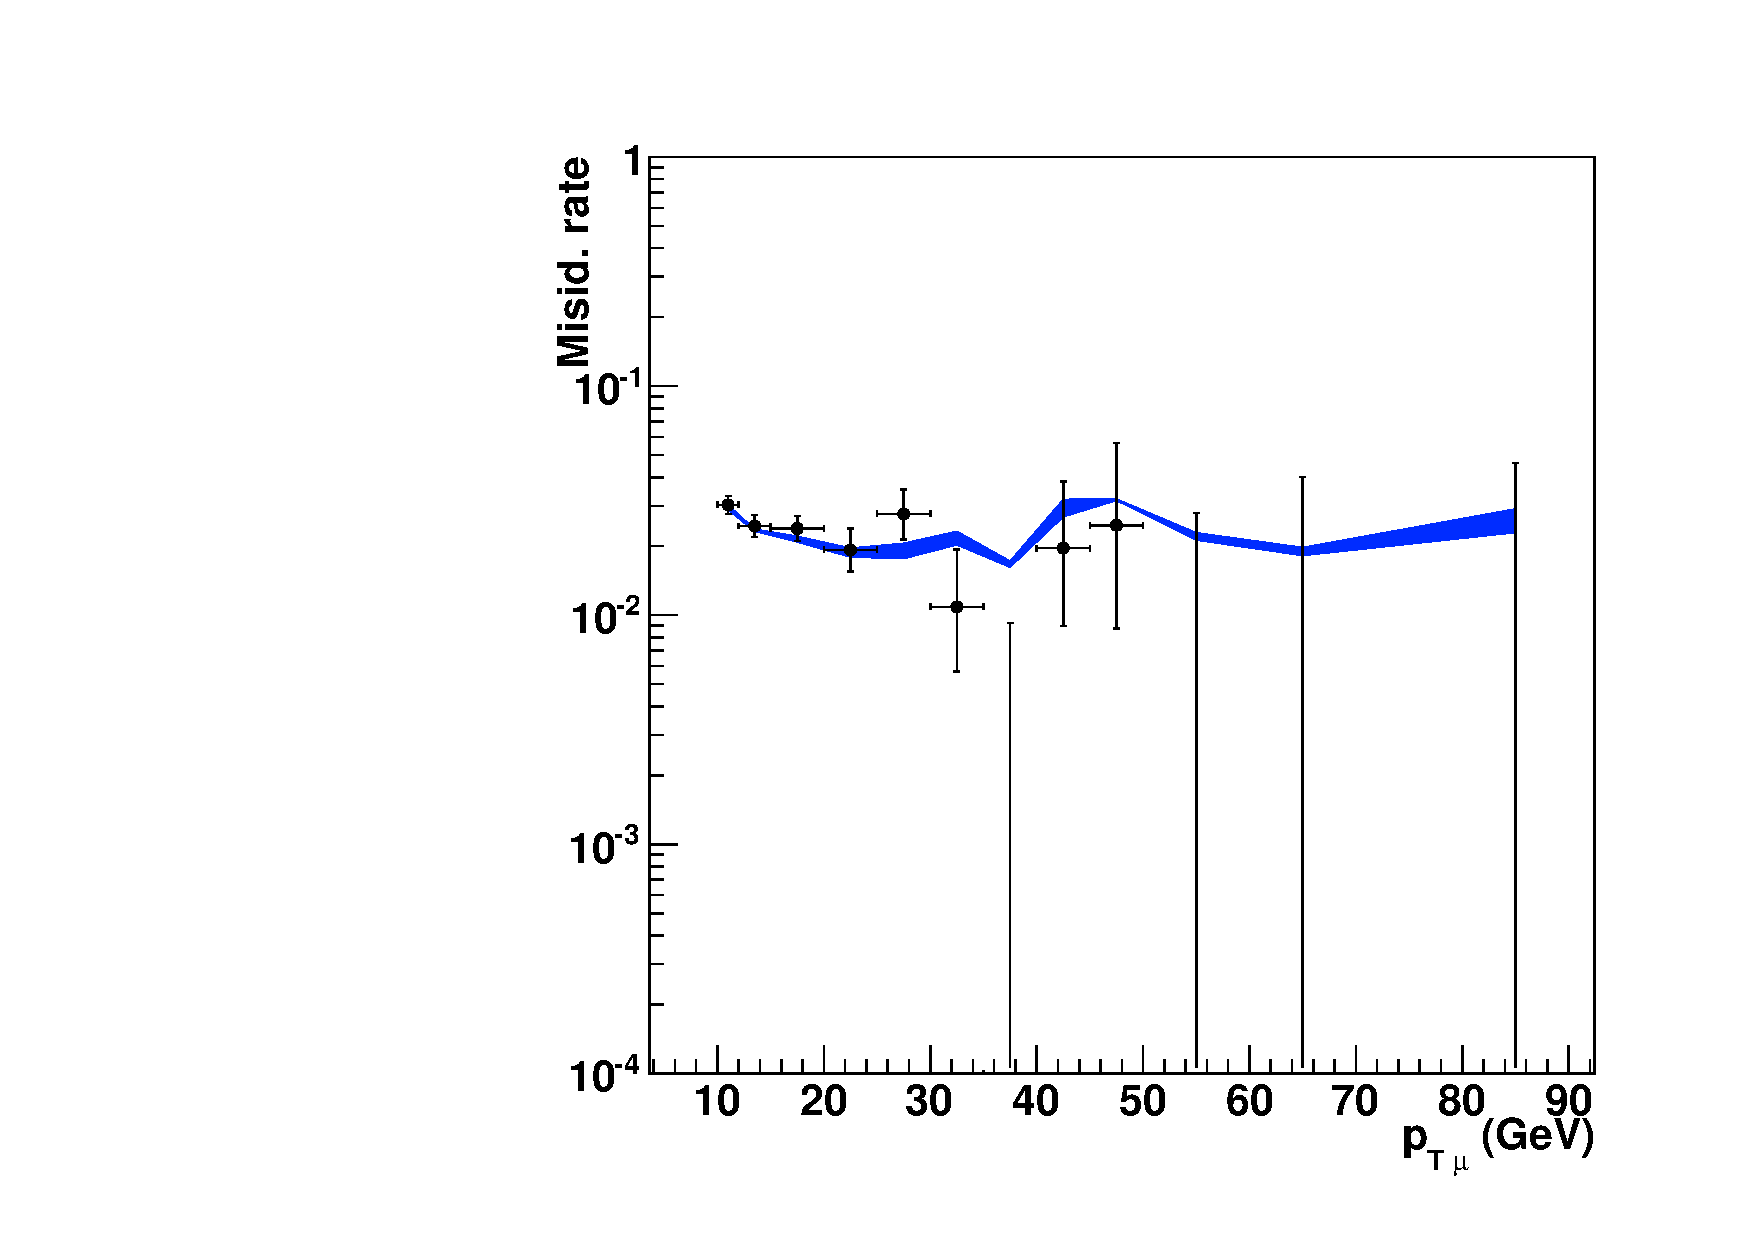
\includegraphics[width=0.49\textwidth]{4_Analisys/pics/8TeV/plots/fakerates/m_mmt_subleading_kNN_muonPt.pdf}\\
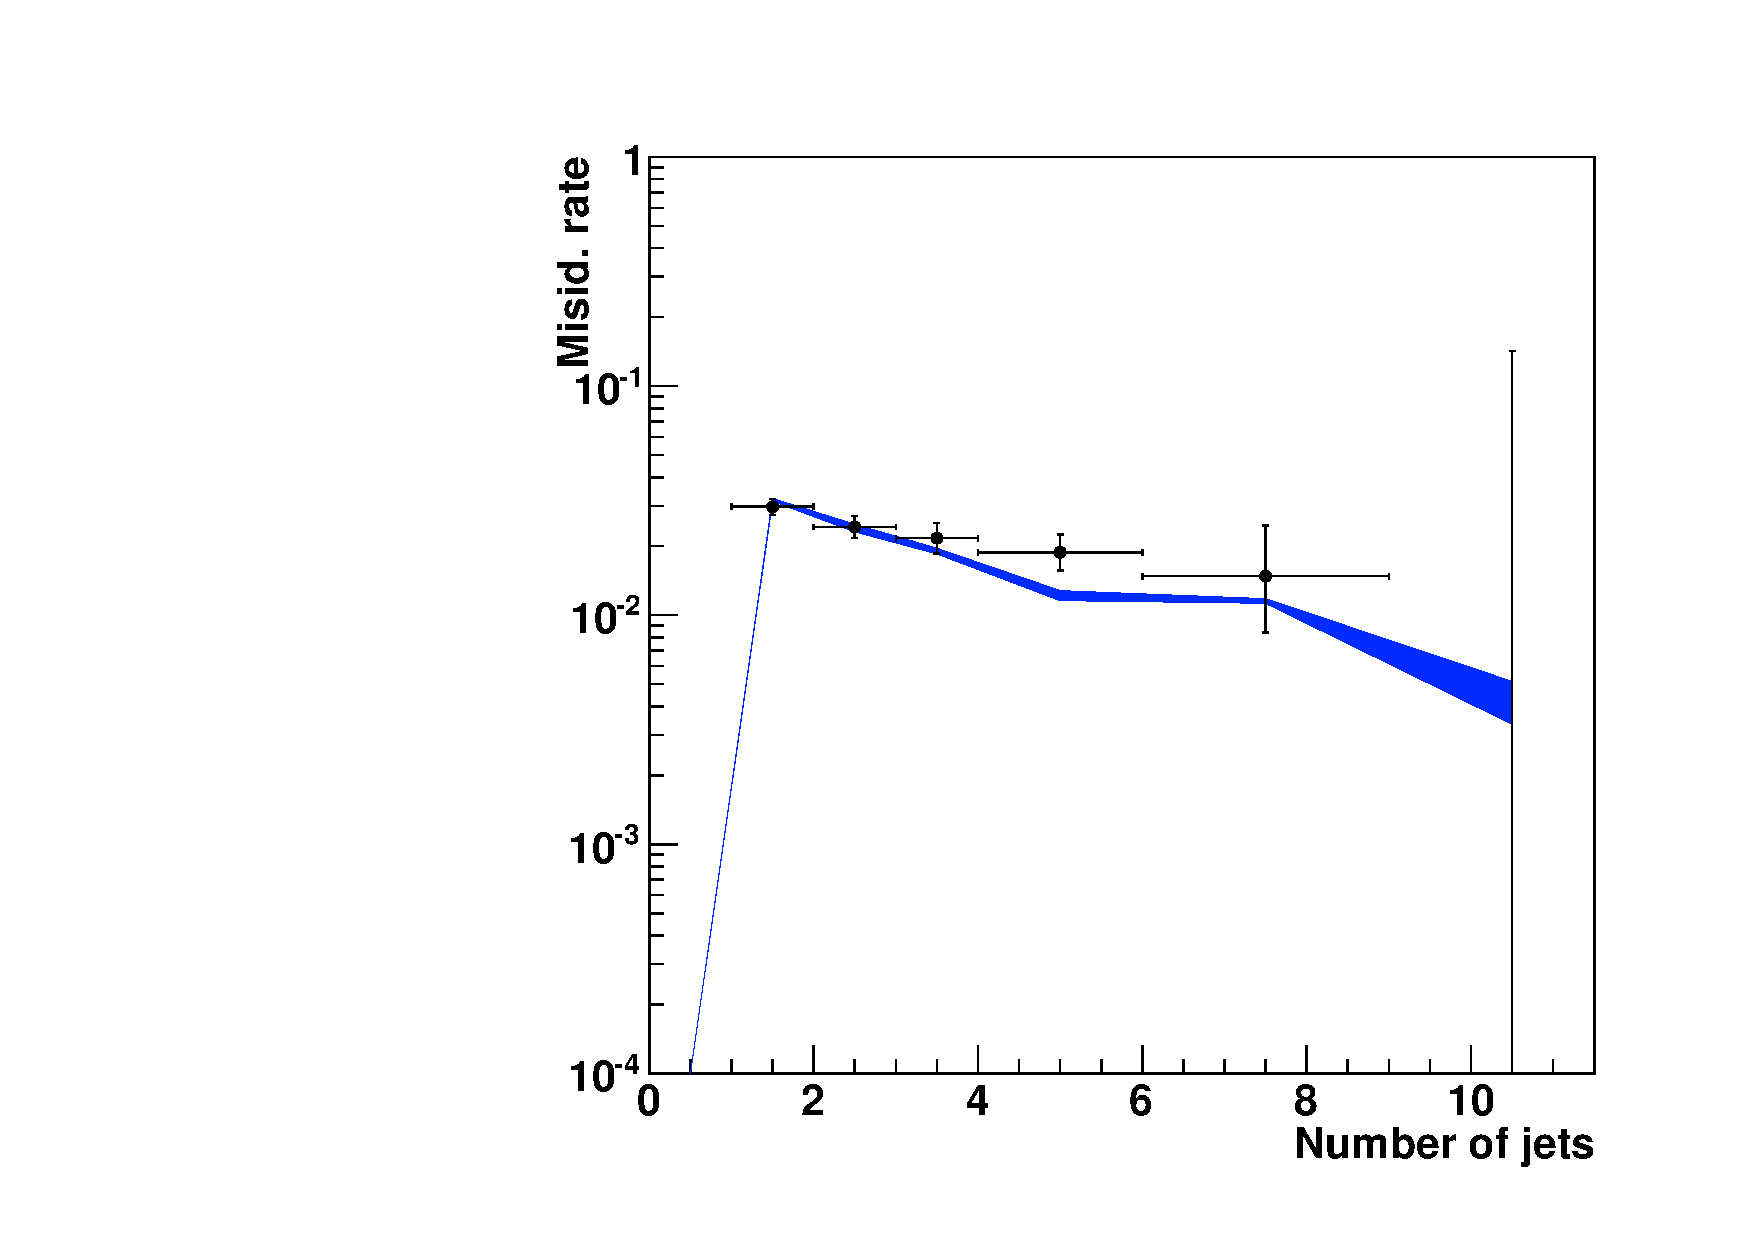
\includegraphics[width=0.49\textwidth]{4_Analisys/pics/8TeV/plots/fakerates/m_mmt_subleading_kNN_numJets20.pdf}
\caption{Measured misidentification probability for sub-leading muons in the training sample dedicated to the $\mu\mu\tau_h$ channel. The blue band represents the output of the kNN algorithm and its related uncertainty.}
\label{fig:fake_rate_sample}
\end{figure}


\subsubsection{Background shape extraction}
The contribution to the signal region from backgrounds containing a given fake object is estimated using an ``anti-isolated'' sideband in which the loose, but \emph{not} the tight, 
selection requirement is satisfied for that object. Events can therefore be divided into three categories:

\begin{enumerate}
\item Events in which the first lepton fails the tight requirements are weighted by $w_1(\vec{x}) = f_1(\vec{x})/(1-f_1(\vec{x}))$
\item Events in which the second lepton fails the tight requirements are weighted by $w_2(\vec{x}) = f_2(\vec{x})/(1-f_2(\vec{x}))$
\item Events in which the both lepton fail the tight requirements are weighted by $w_1(\vec{x}) \cdot w_2(\vec{x})$
\end{enumerate}

Each weighted category represents the contribution to the signal region of the backgrounds in which jets fake one or both the light leptons. As the events 
in which both reconstructed leptons are due to $\rm{jet}\To\ell$ fakes %where jets are mis-reconstructed as both leptons 
are included in category 1 as well as in category 2, it is necessary to remove the double-counting by subtracting the weighted events of category three, obtaining:

\begin{equation}
N_{bkg} = N_1 + N_2 - N_3
\end{equation}

where $N_{bkg}$ denotes the final estimate for the number of background events in the signal region and $N_i$ denotes the scaled number events in category $i$.

%Sys uncertainty
Uncertainties on the kNN training, evaluated as described above, are propagated to the background estimate for the signal region by comparing %computing 
the event weights obtained with classifiers trained with the central value and with the two one-sigma boundaries. The difference is taken as systematic uncertainty.

%Empty bins
In rare cases, especially in the tail of kinematic distributions, statistical fluctuations cause the number of weighted events in category three to exceed the sum of $N_1 + N_2$, %the other two categories, 
and therefore the expected yield in the signal region becomes negative. In these cases the yield is set to the value of category three only, relying on the much larger statistics present in that sideband.


%

\subsection{Validation of the fake lepton method}
\label{sec:f3_validation}

The method for estimating the reducible backgrounds is validated in two control regions which are dominated by fake $\tau_h$ candidates.
%This exercises all mechanisms of the reducible background estimation, since the $\tau_h$ candidate never participates in the misidentification rate method.
These control regions provide an independent validation, as they are naturally exclusive with respect to the event sample used to train the kNN. Events in the control region are selected by maintaining
the light-lepton same-charge requirement, but inverting the isolation requirement of the $\tau_h$ candidate and in one of the regions the charge of the tau is furthermore required to be the same as the leptons.
This regions are dominated by W+Jets and $t\anti{t}$ backgrounds.
Comparison between the observed and predicted kinematic distributions in the control regions is shown for the $\mu\mu\tau_h$, $e\mu\tau_h$ and $ee\tau_h$ channels in figures~\ref{fig:LLT_mmt_f3_control_7TeV}--\ref{fig:LLT_eet_f3_control_8TeV} respectively.
Reasonable agreement is observed, considering that the expected background in this region lacks an additional systematic uncertainty, described in the next section and not defined in this region, which has sizable effect both on the distribution and total normalization of the reducible background.

\begin{figure}
\begin{center}
  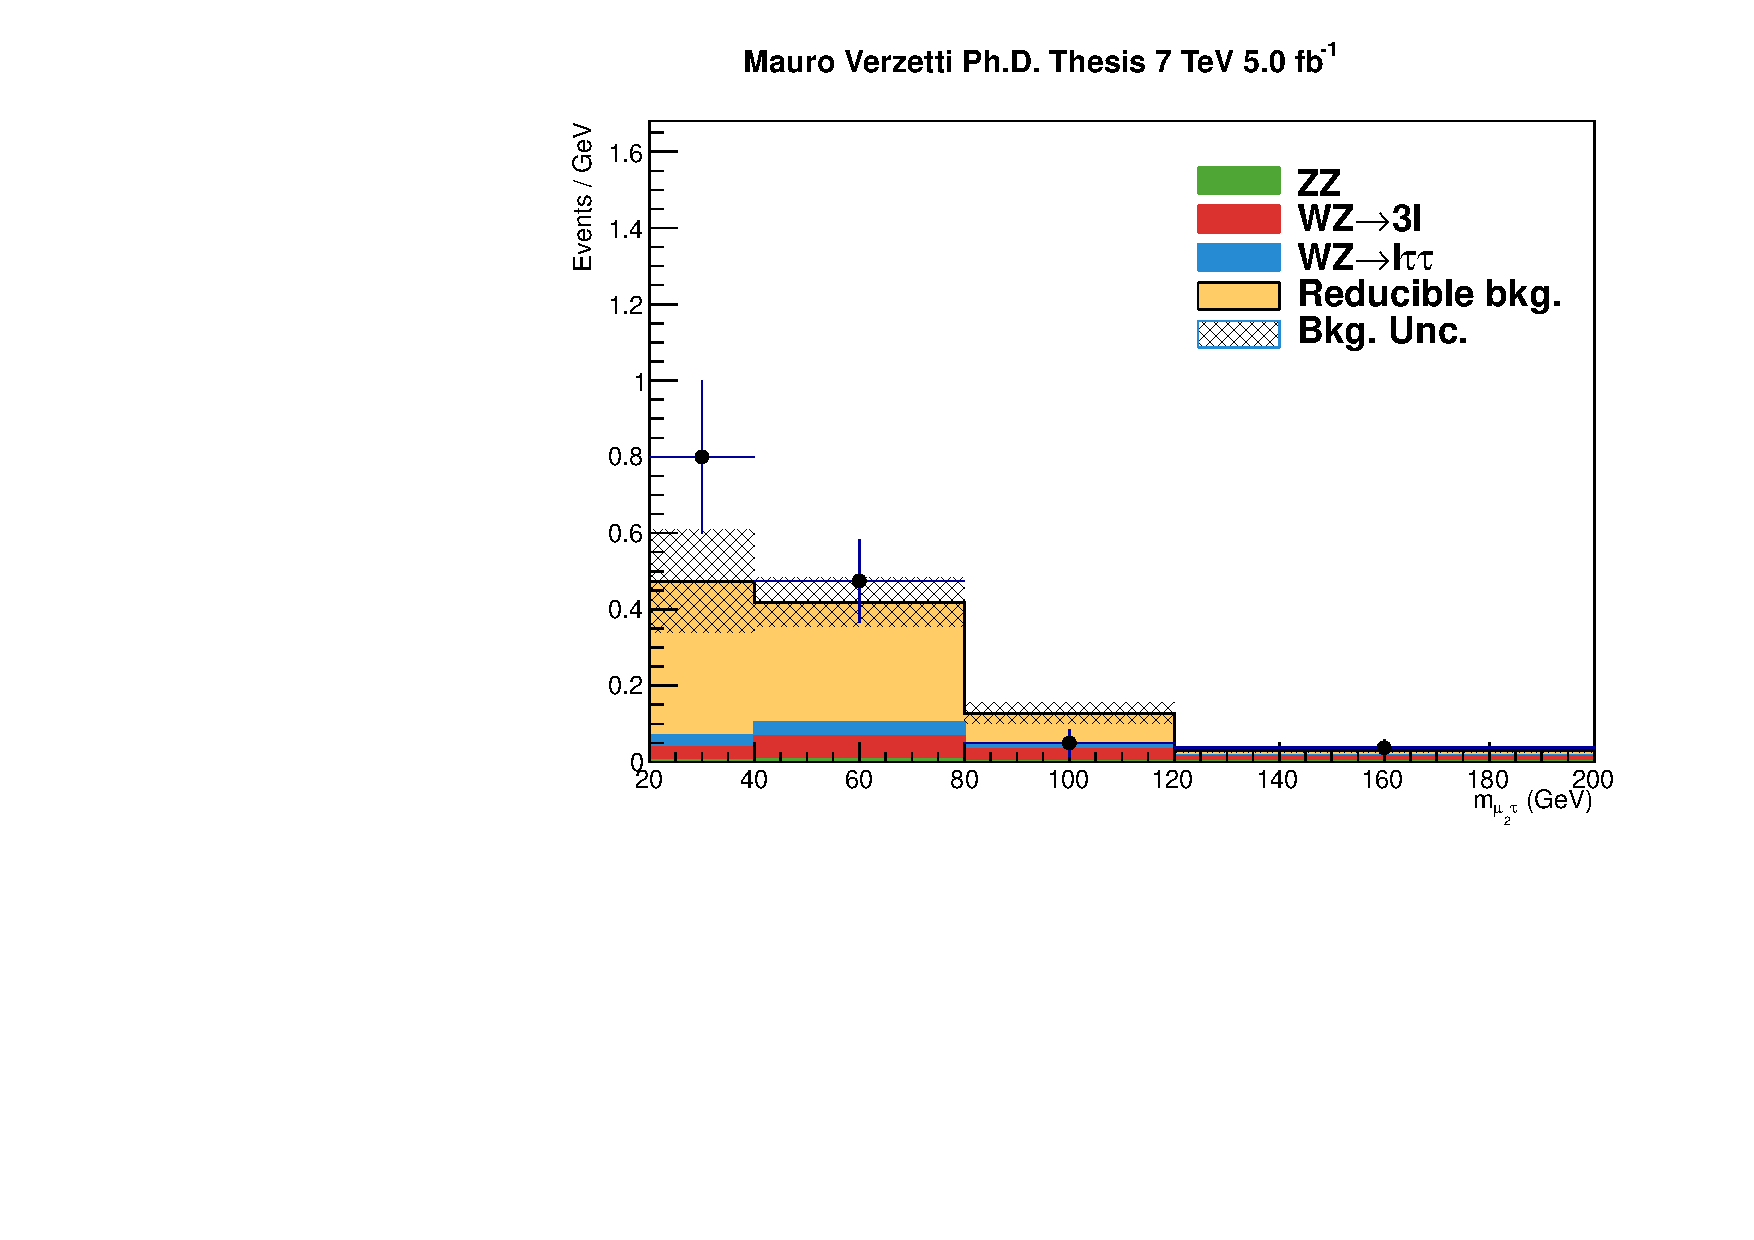
\includegraphics[width=0.49\textwidth]{4_Analisys/pics/7TeV/plots/mmt/f3/Full/final-f3-subMass-Full.pdf}
  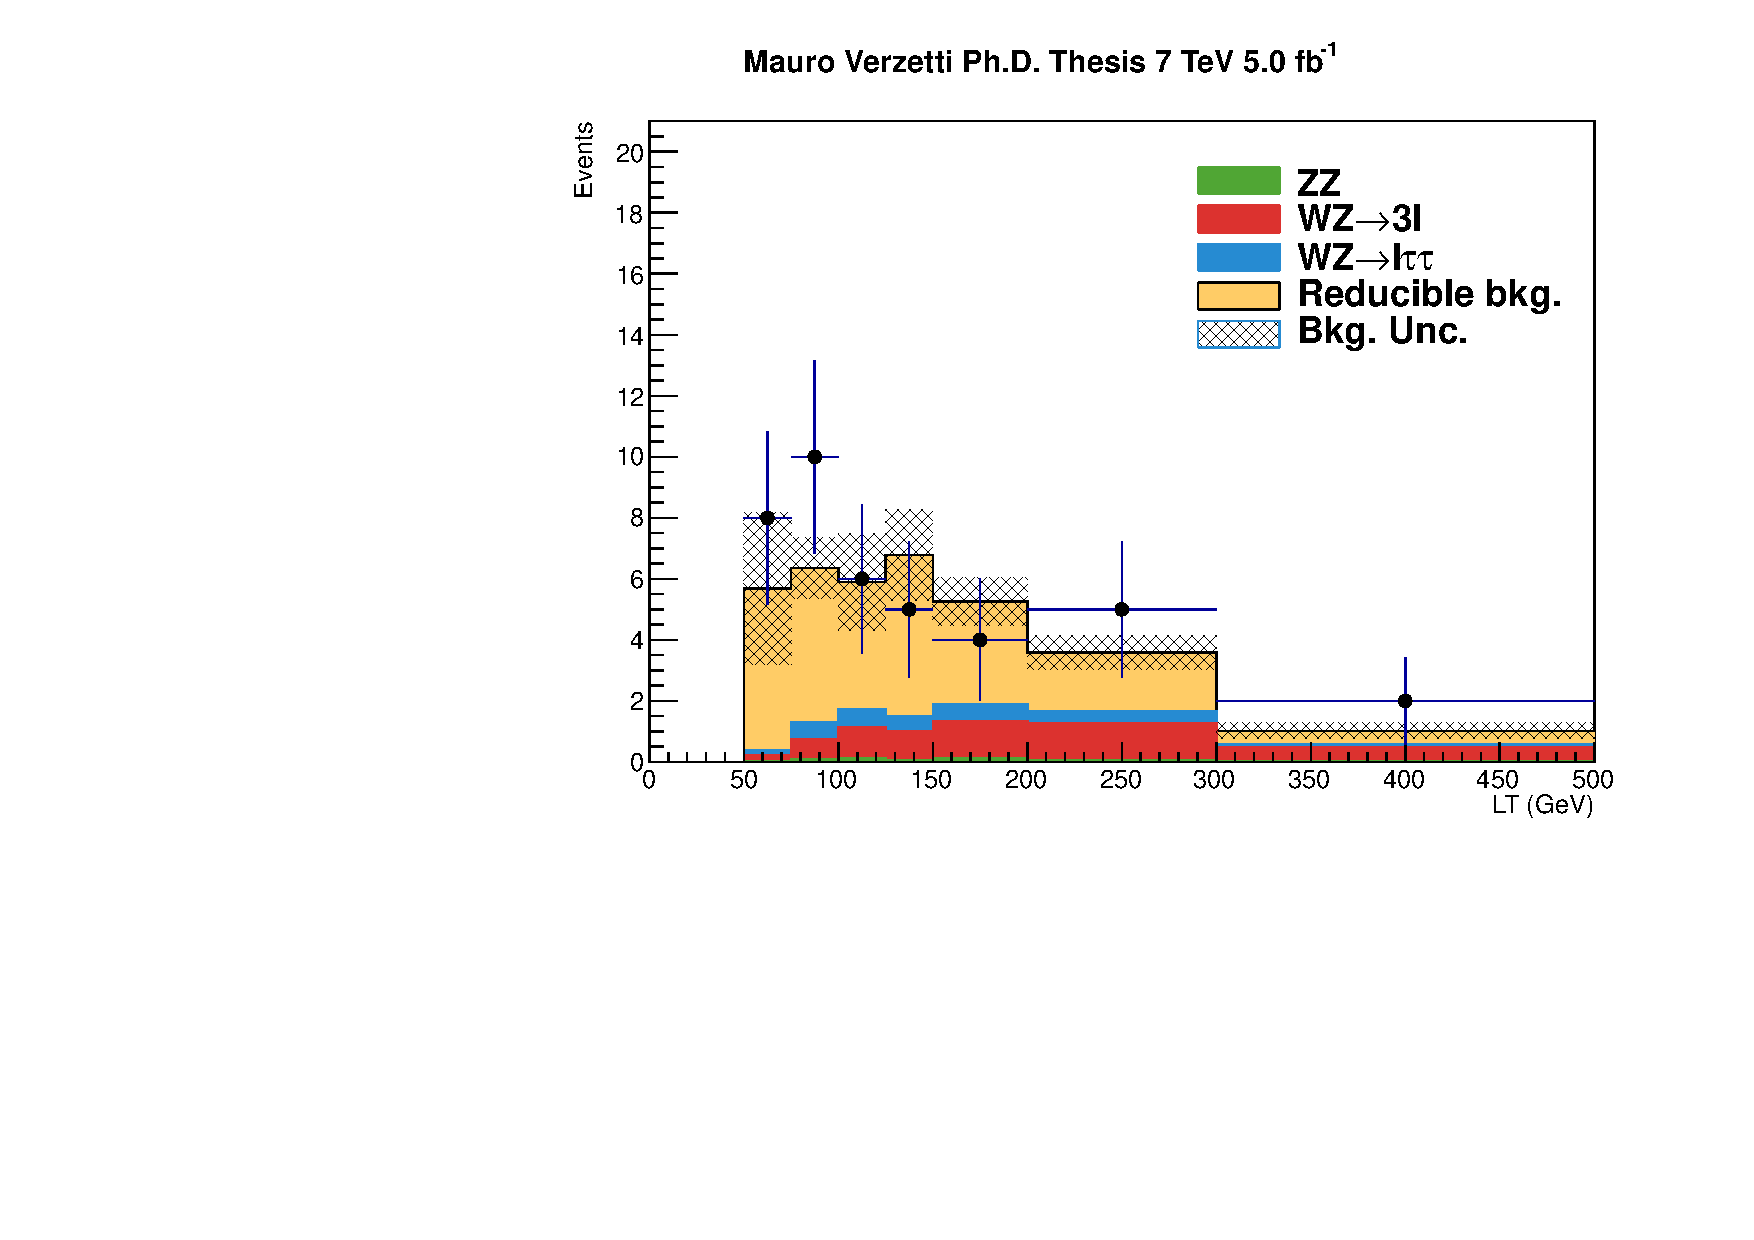
\includegraphics[width=0.49\textwidth]{4_Analisys/pics/7TeV/plots/mmt/f3/final-LT.pdf}\\
  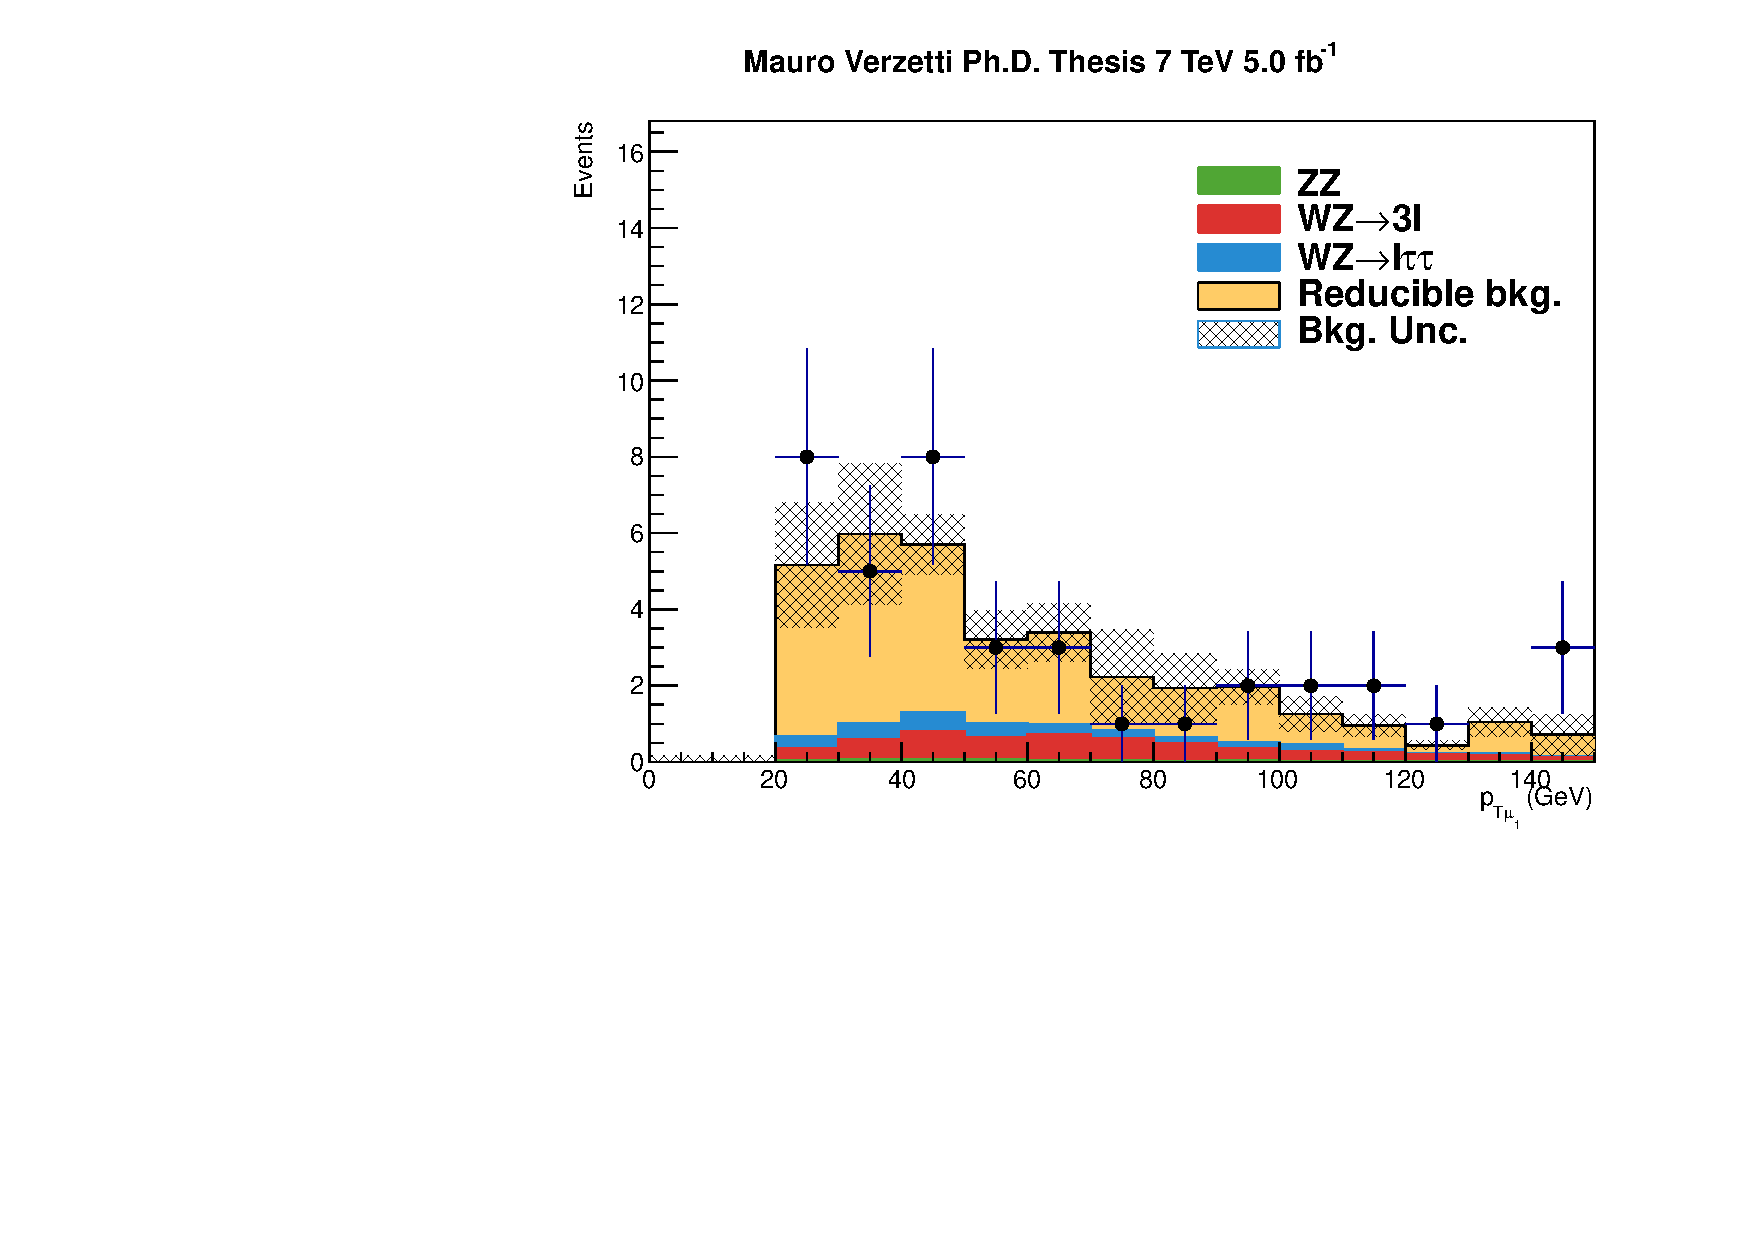
\includegraphics[width=0.49\textwidth]{4_Analisys/pics/7TeV/plots/mmt/f3/Full/final-f3-m1Pt-Full.pdf}
  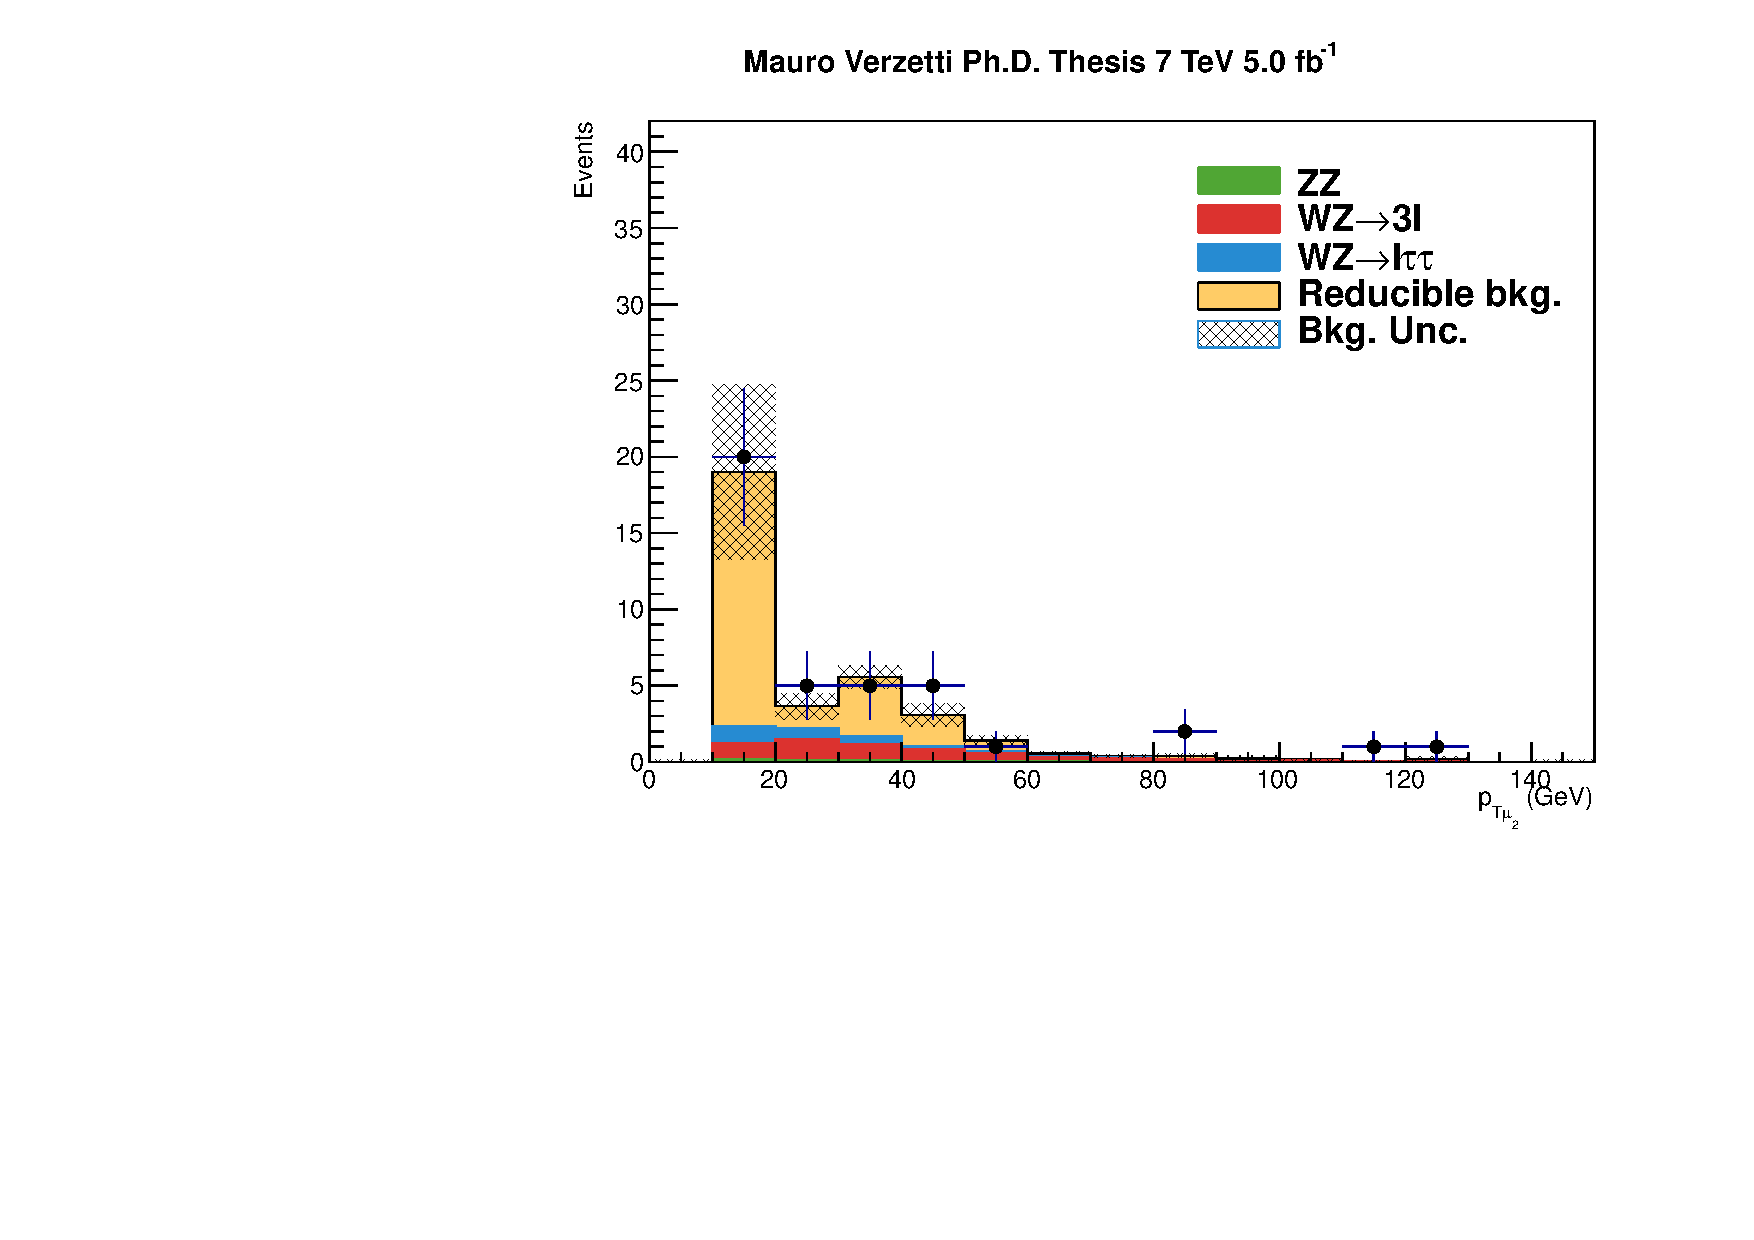
\includegraphics[width=0.49\textwidth]{4_Analisys/pics/7TeV/plots/mmt/f3/Full/final-f3-m2Pt-Full.pdf}\\
  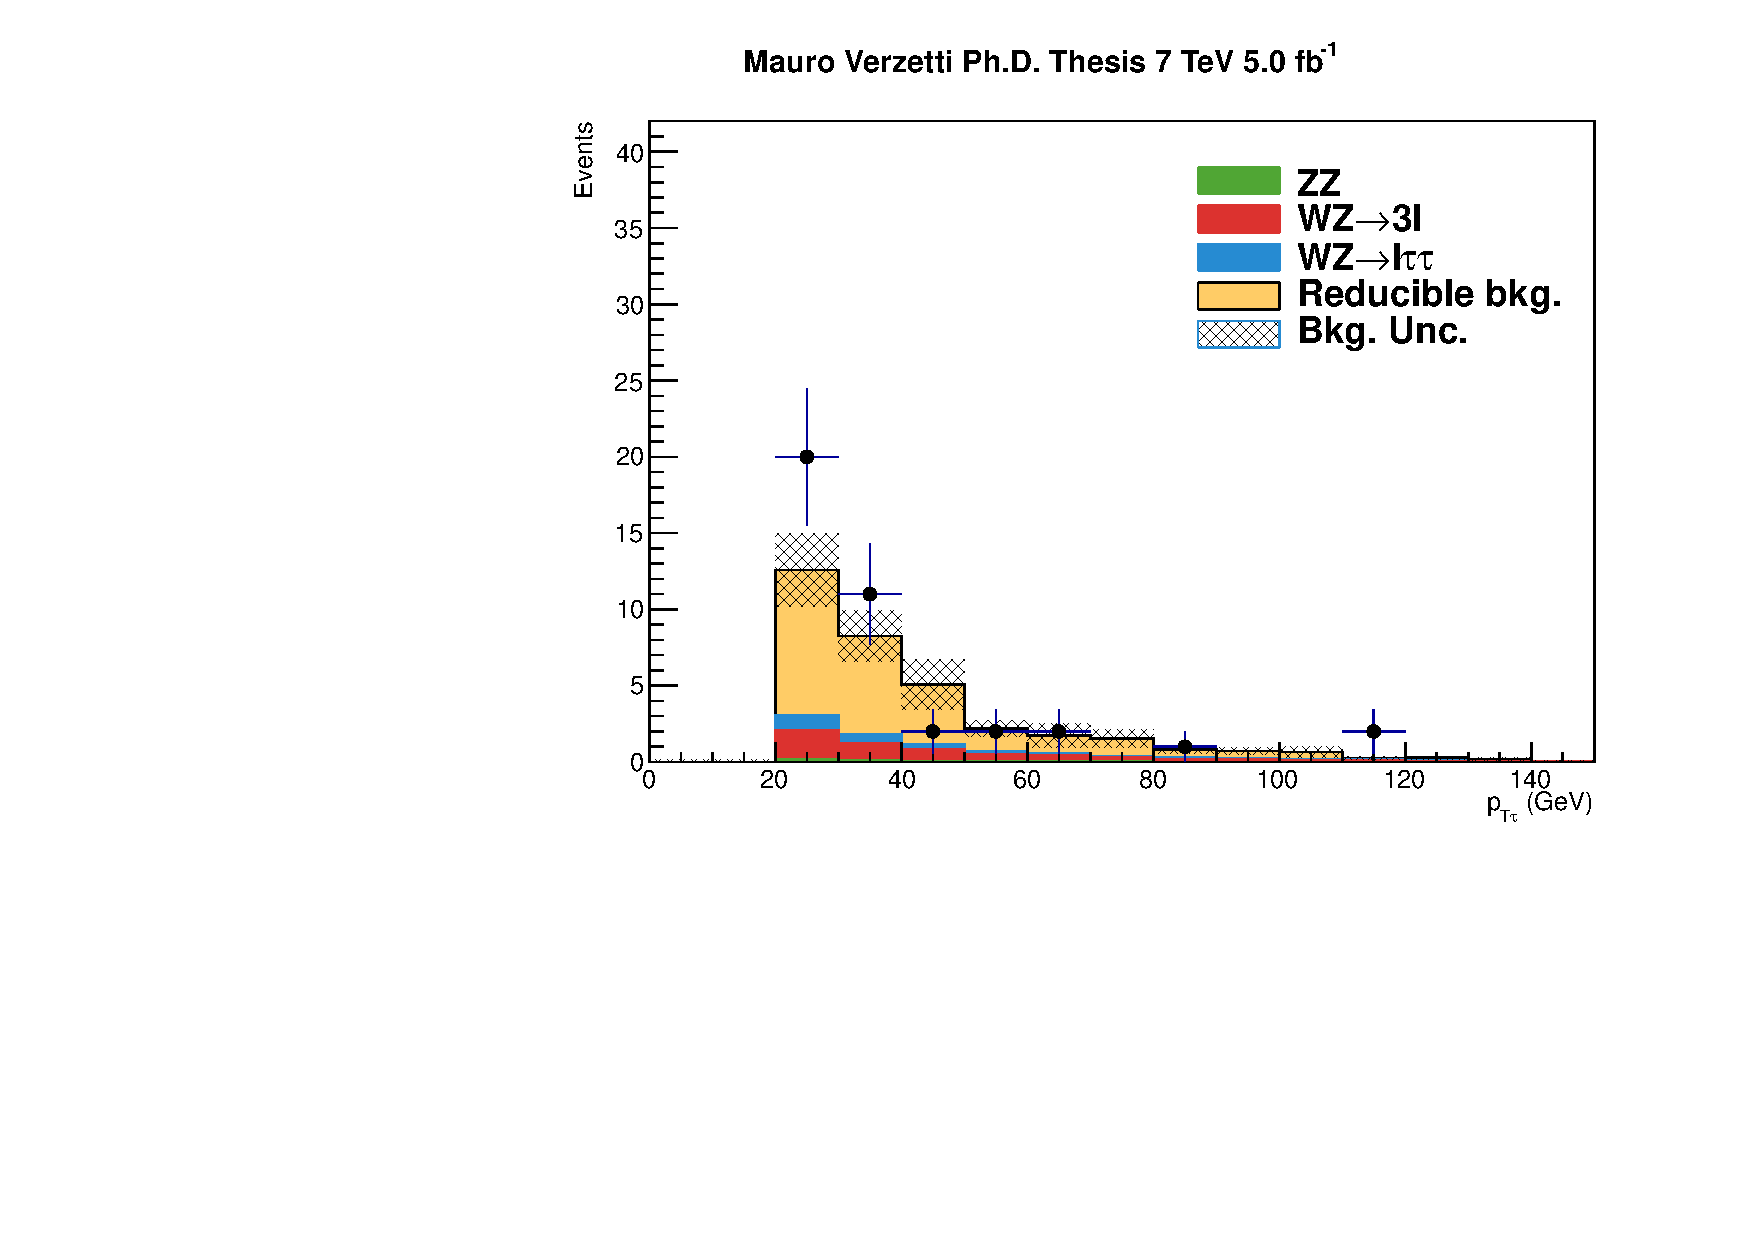
\includegraphics[width=0.49\textwidth]{4_Analisys/pics/7TeV/plots/mmt/f3/Full/final-f3-tPt-Full.pdf}
  \caption{Comparison of measured and predicted backgrounds in the $\mu\mu\tau_h$ ``fake tau'' control region for 7 TeV data.
  From top left to bottom: mass of the sub-leading muon and the tau system, scalar sum of the leptons \pT ($L_T$), \pT of the leading and sub-leading muon, and \pT of the hadronic tau.
  The reducible background contribution is estimated by the kNN method, as in the signal region.
  The shaded band represents the uncertainty on the sum of the background contributions.
  }
  \label{fig:LLT_mmt_f3_control_7TeV}
\end{center}
\end{figure}

\begin{figure}
\begin{center}
  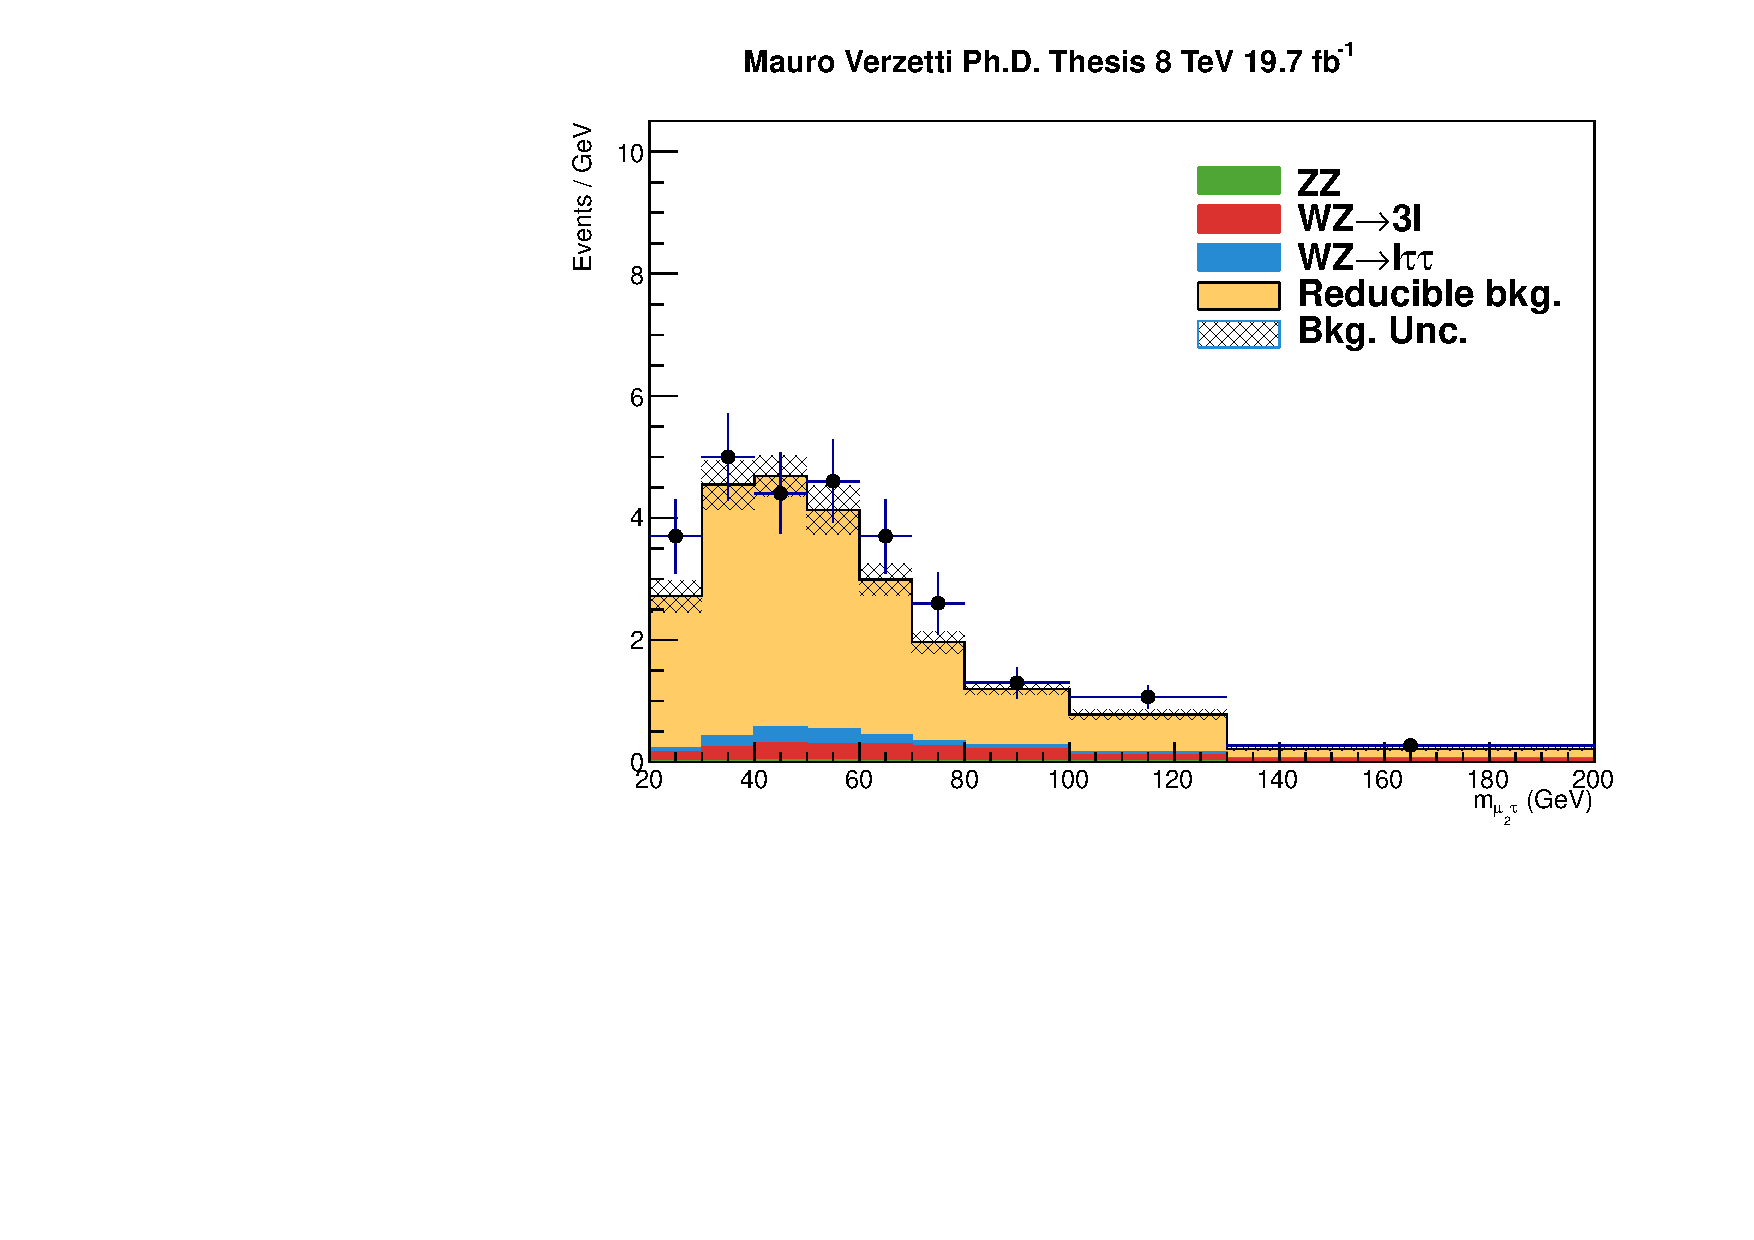
\includegraphics[width=0.49\textwidth]{4_Analisys/pics/8TeV/plots/mmt/f3/Full/final-f3-subMass-Full.pdf}
  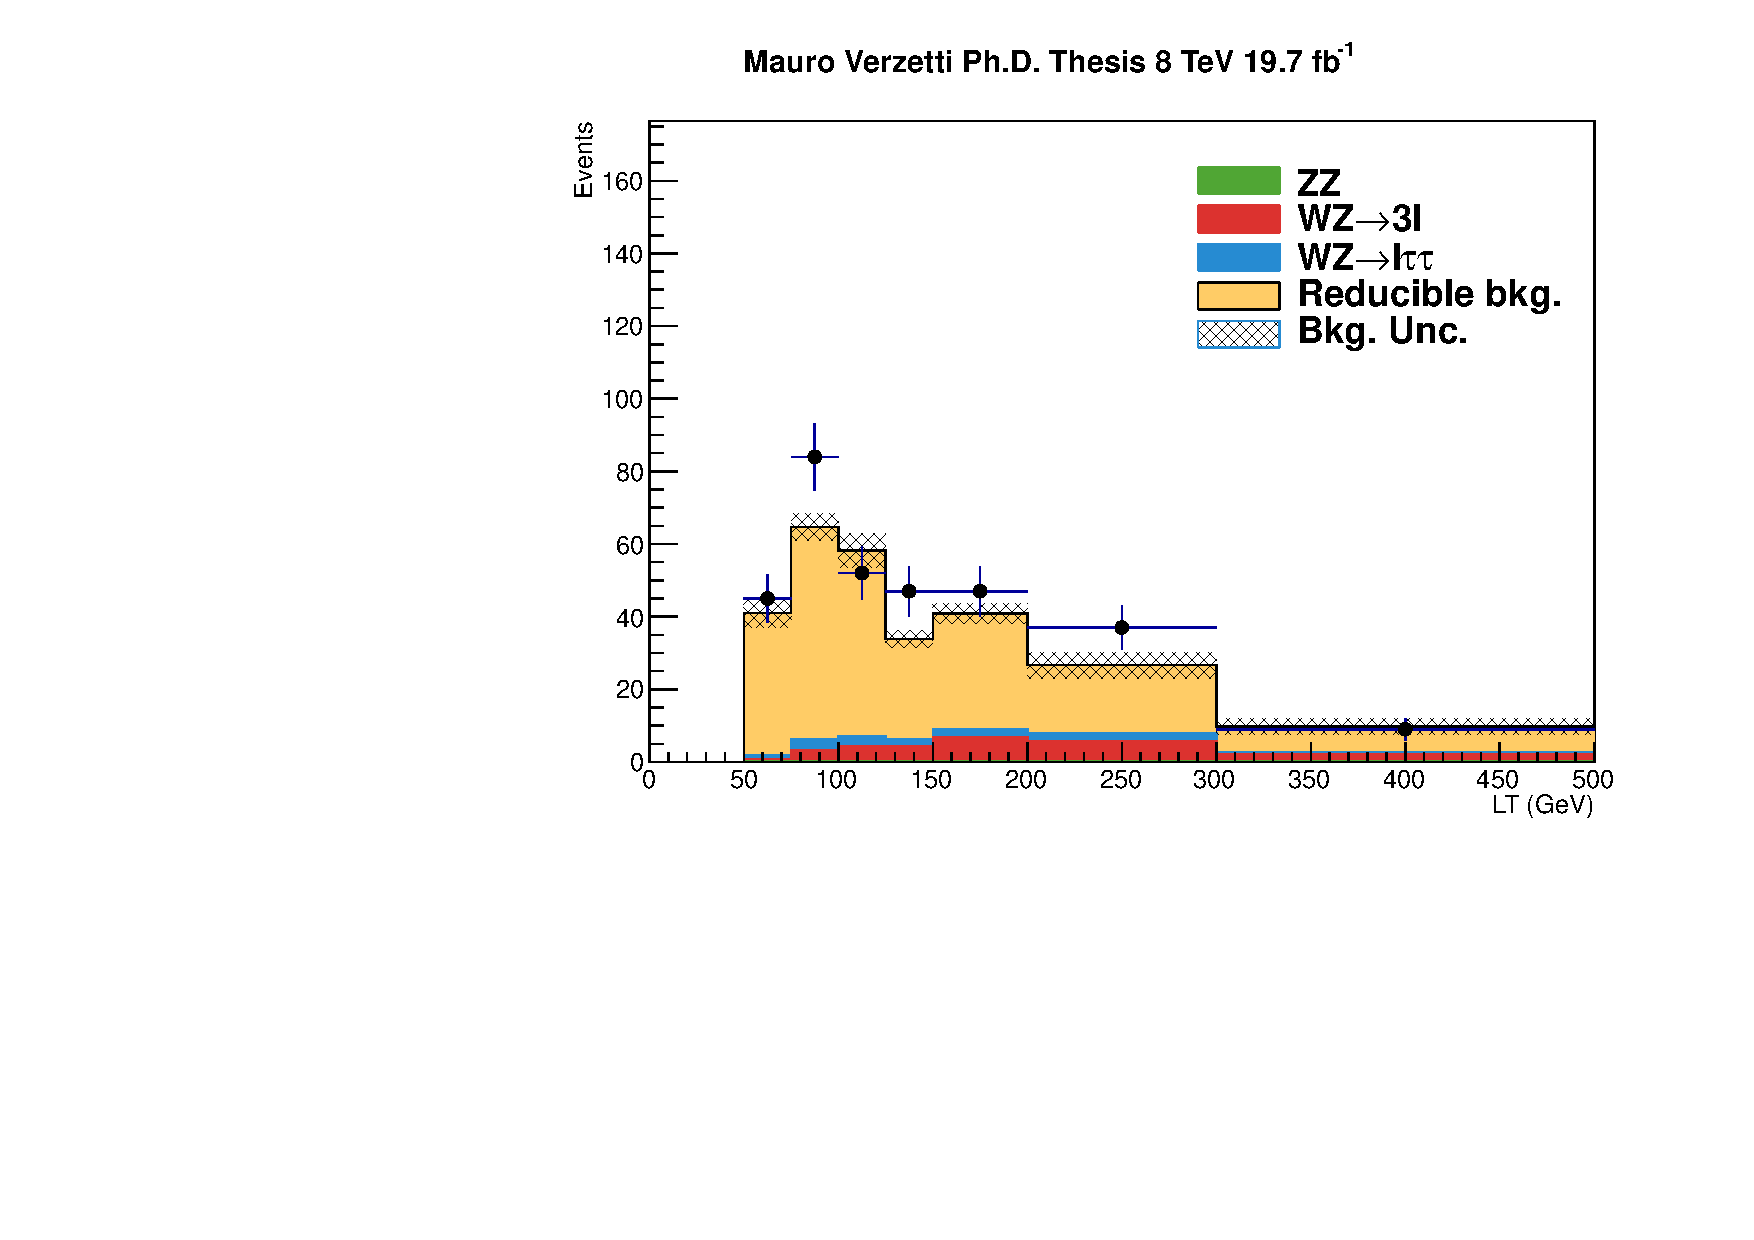
\includegraphics[width=0.49\textwidth]{4_Analisys/pics/8TeV/plots/mmt/f3/final-LT.pdf}\\
  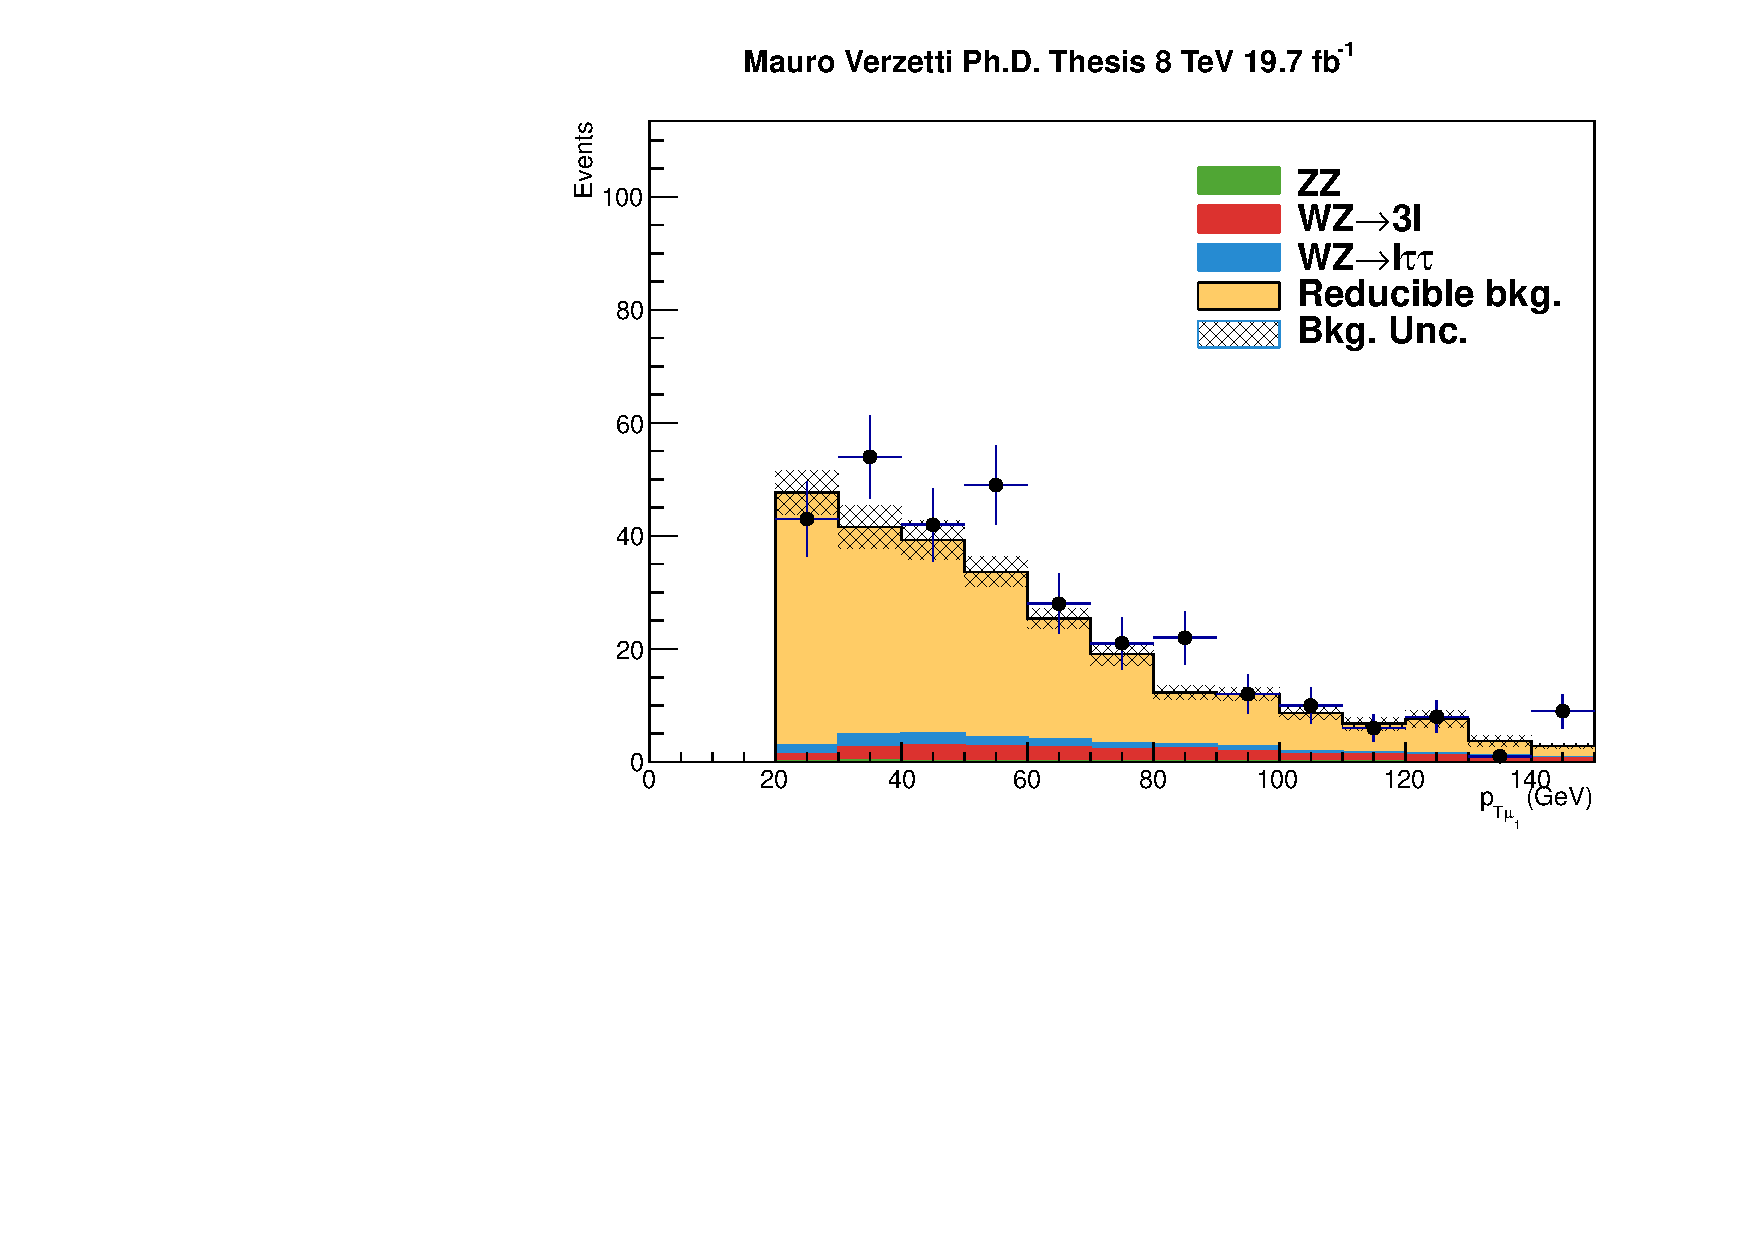
\includegraphics[width=0.49\textwidth]{4_Analisys/pics/8TeV/plots/mmt/f3/Full/final-f3-m1Pt-Full.pdf}
  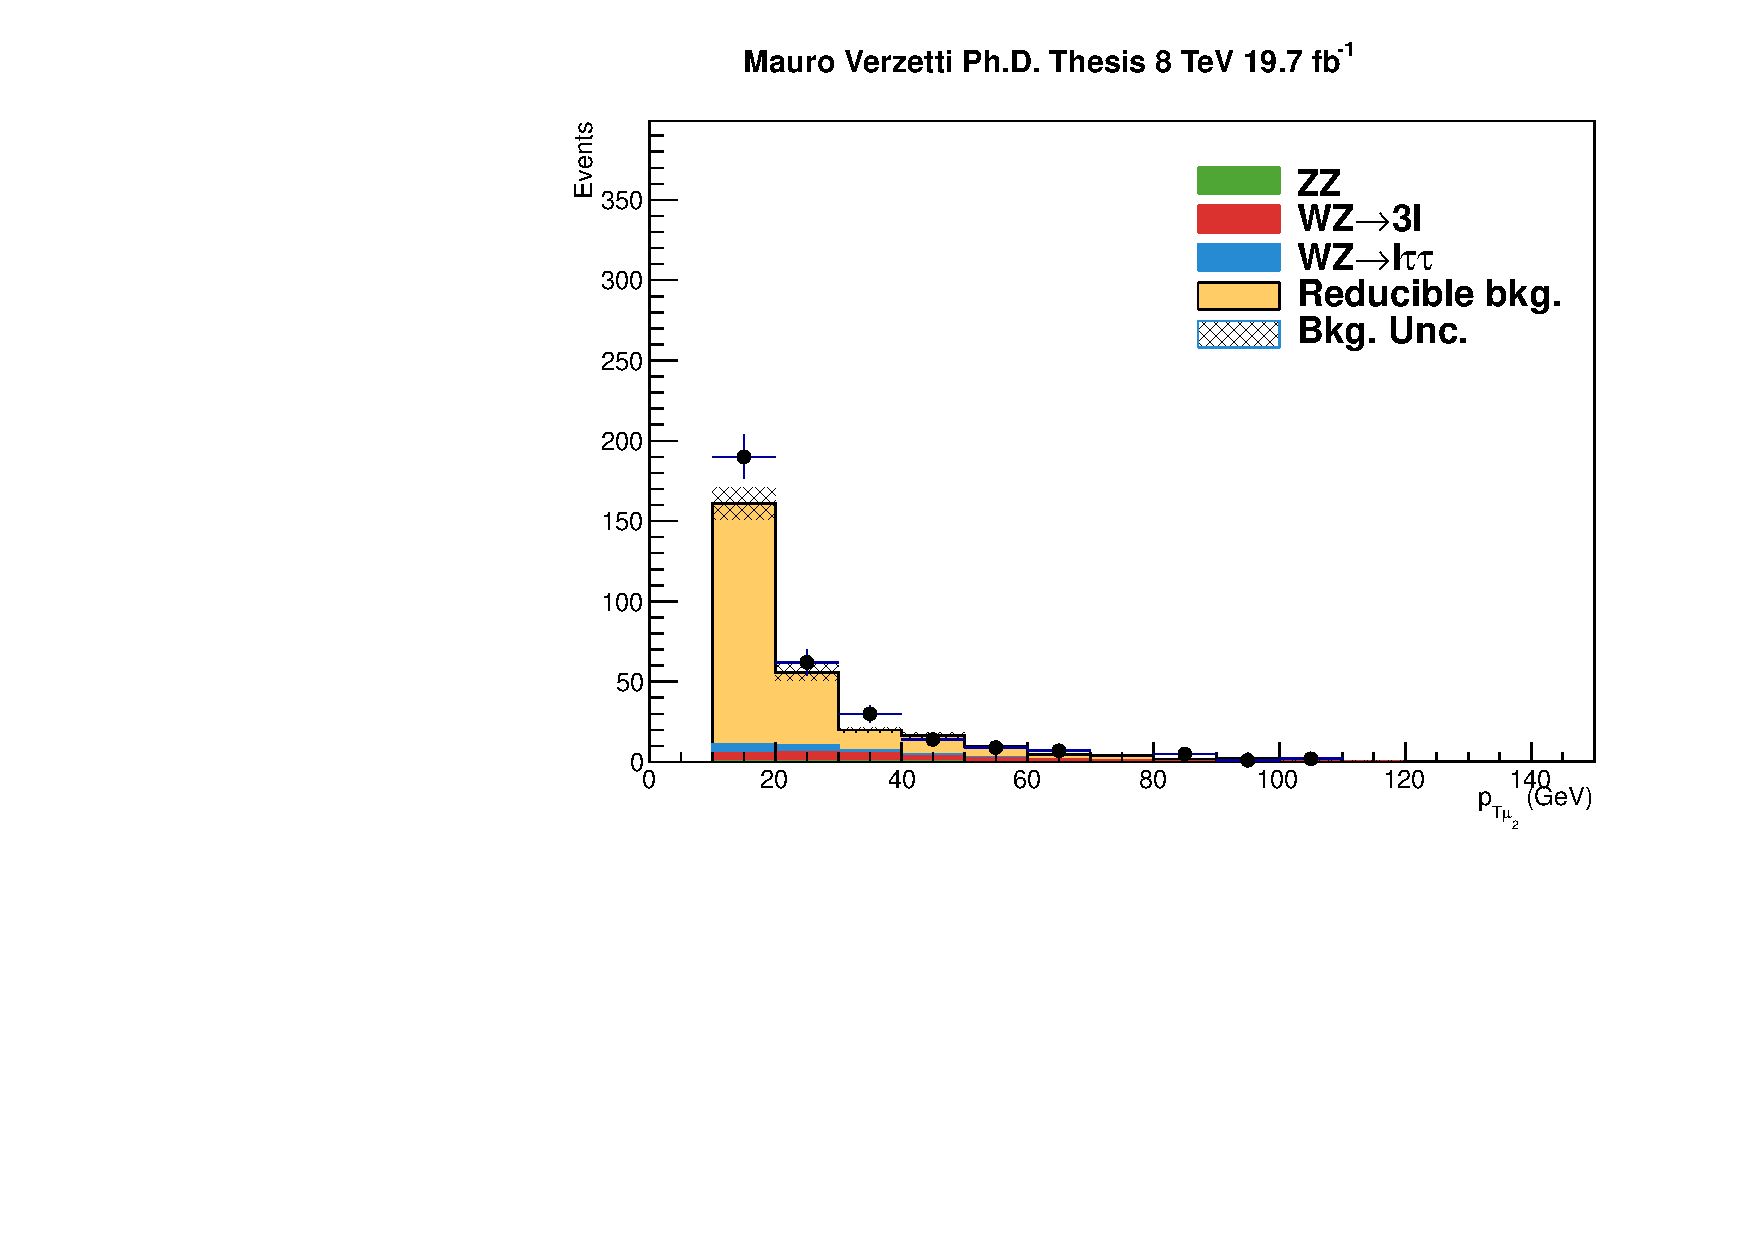
\includegraphics[width=0.49\textwidth]{4_Analisys/pics/8TeV/plots/mmt/f3/Full/final-f3-m2Pt-Full.pdf}\\
  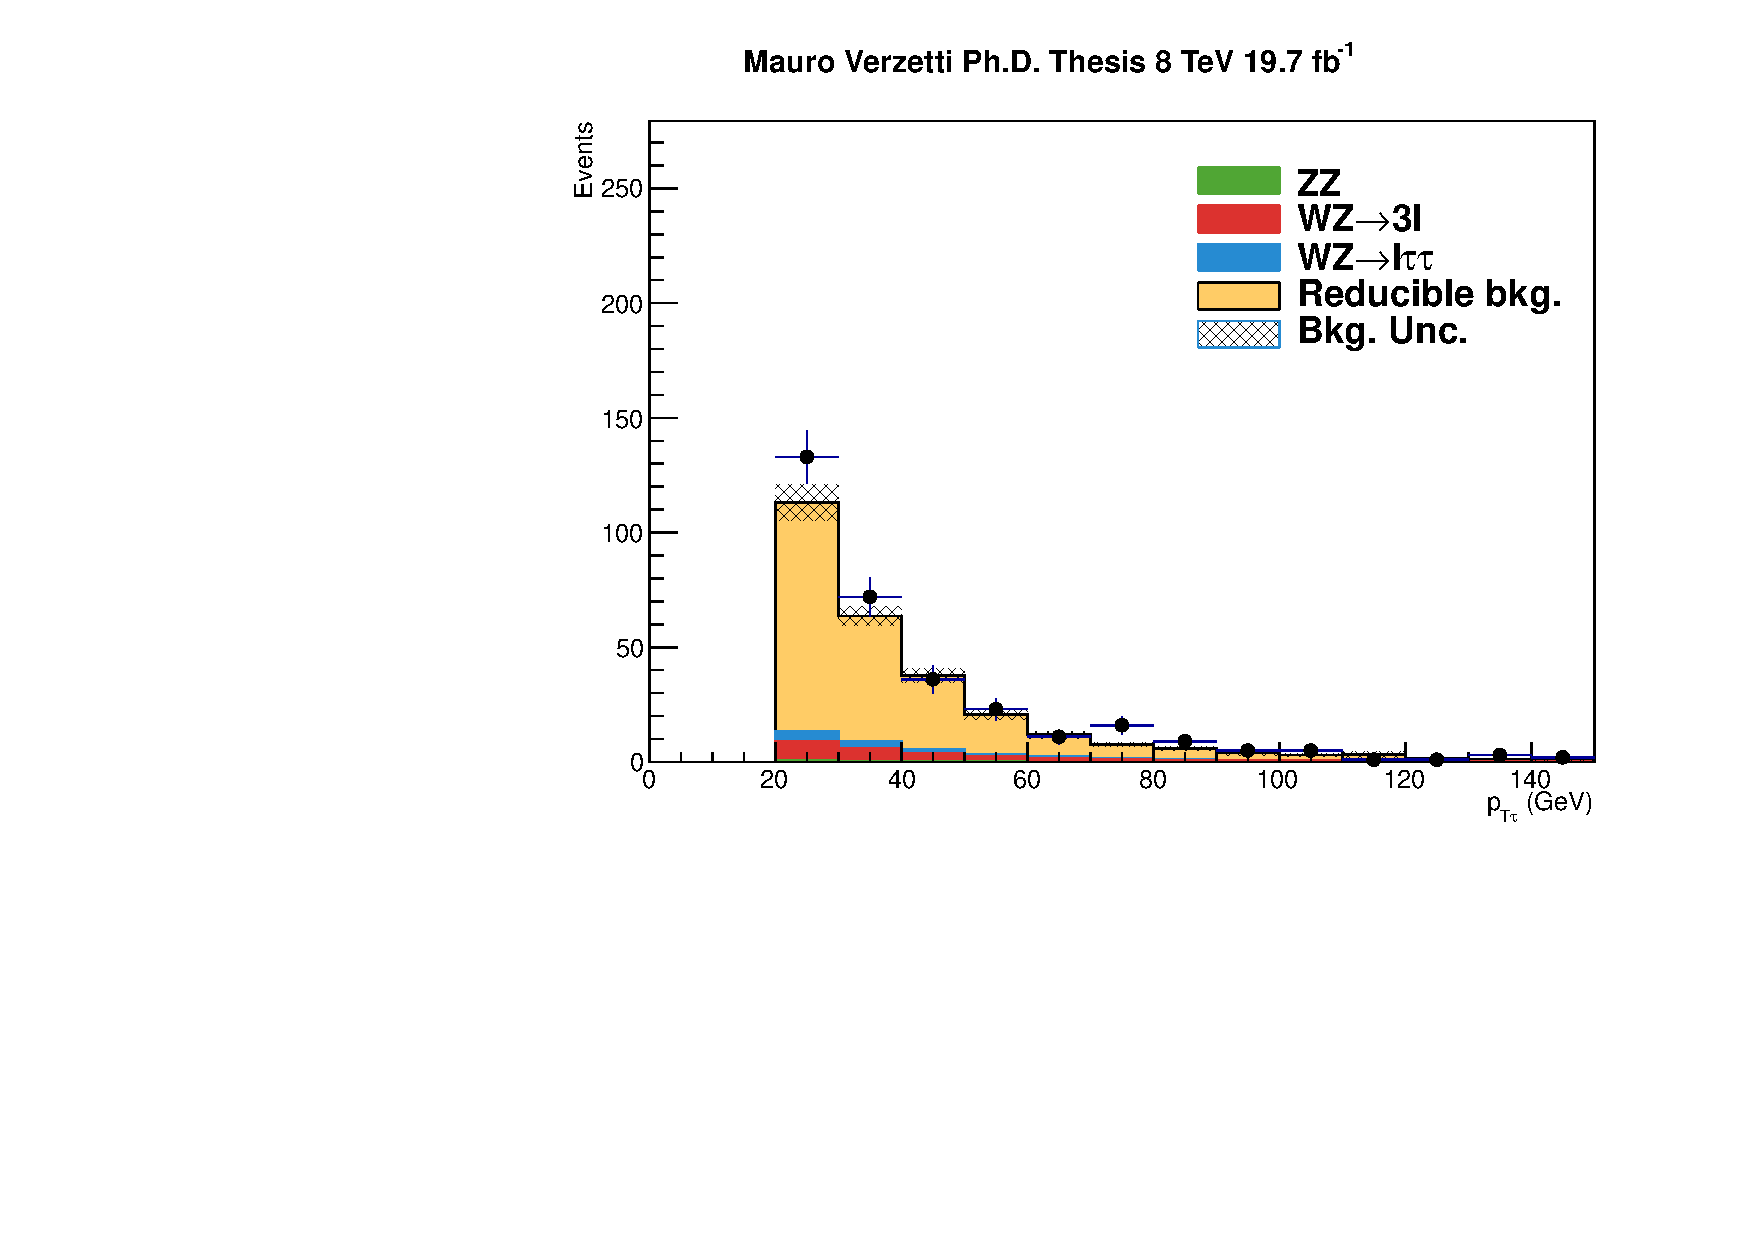
\includegraphics[width=0.49\textwidth]{4_Analisys/pics/8TeV/plots/mmt/f3/Full/final-f3-tPt-Full.pdf}
  \caption{Comparison of measured and predicted backgrounds in the $\mu\mu\tau_h$ ``fake tau'' control region for 8 TeV data.
  From top left to bottom: mass of the sub-leading muon and the tau system, scalar sum of the leptons \pT ($L_T$), \pT of the leading and sub-leading muon, and \pT of the hadronic tau.
  The reducible background contribution is estimated by the kNN method, as in the signal region.
  The shaded band represents the uncertainty on the sum of the background contributions.
  }
  \label{fig:LLT_mmt_f3_control_8TeV}
\end{center}
\end{figure}

\begin{figure}
\begin{center}
  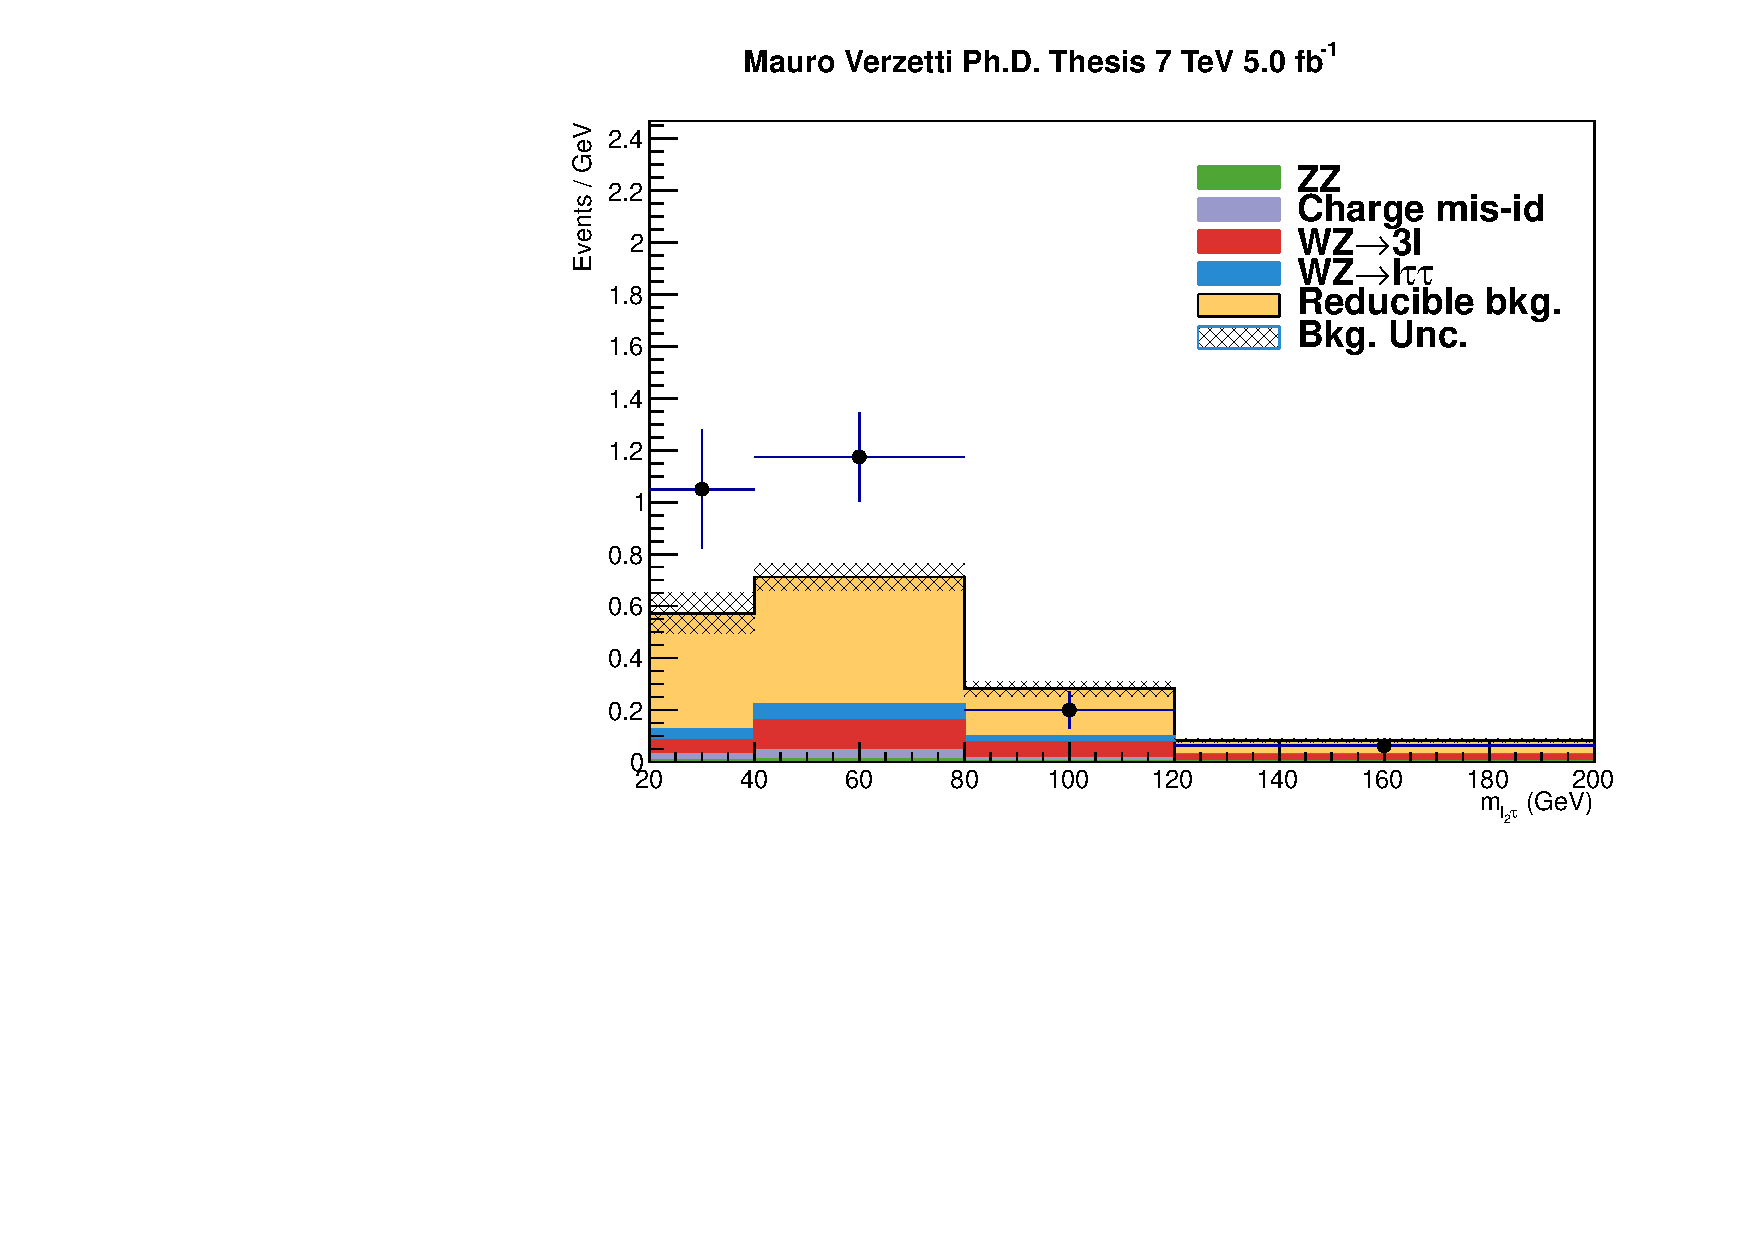
\includegraphics[width=0.49\textwidth]{4_Analisys/pics/7TeV/plots/emt/f3/Full/final-f3-subMass-Full.pdf}
  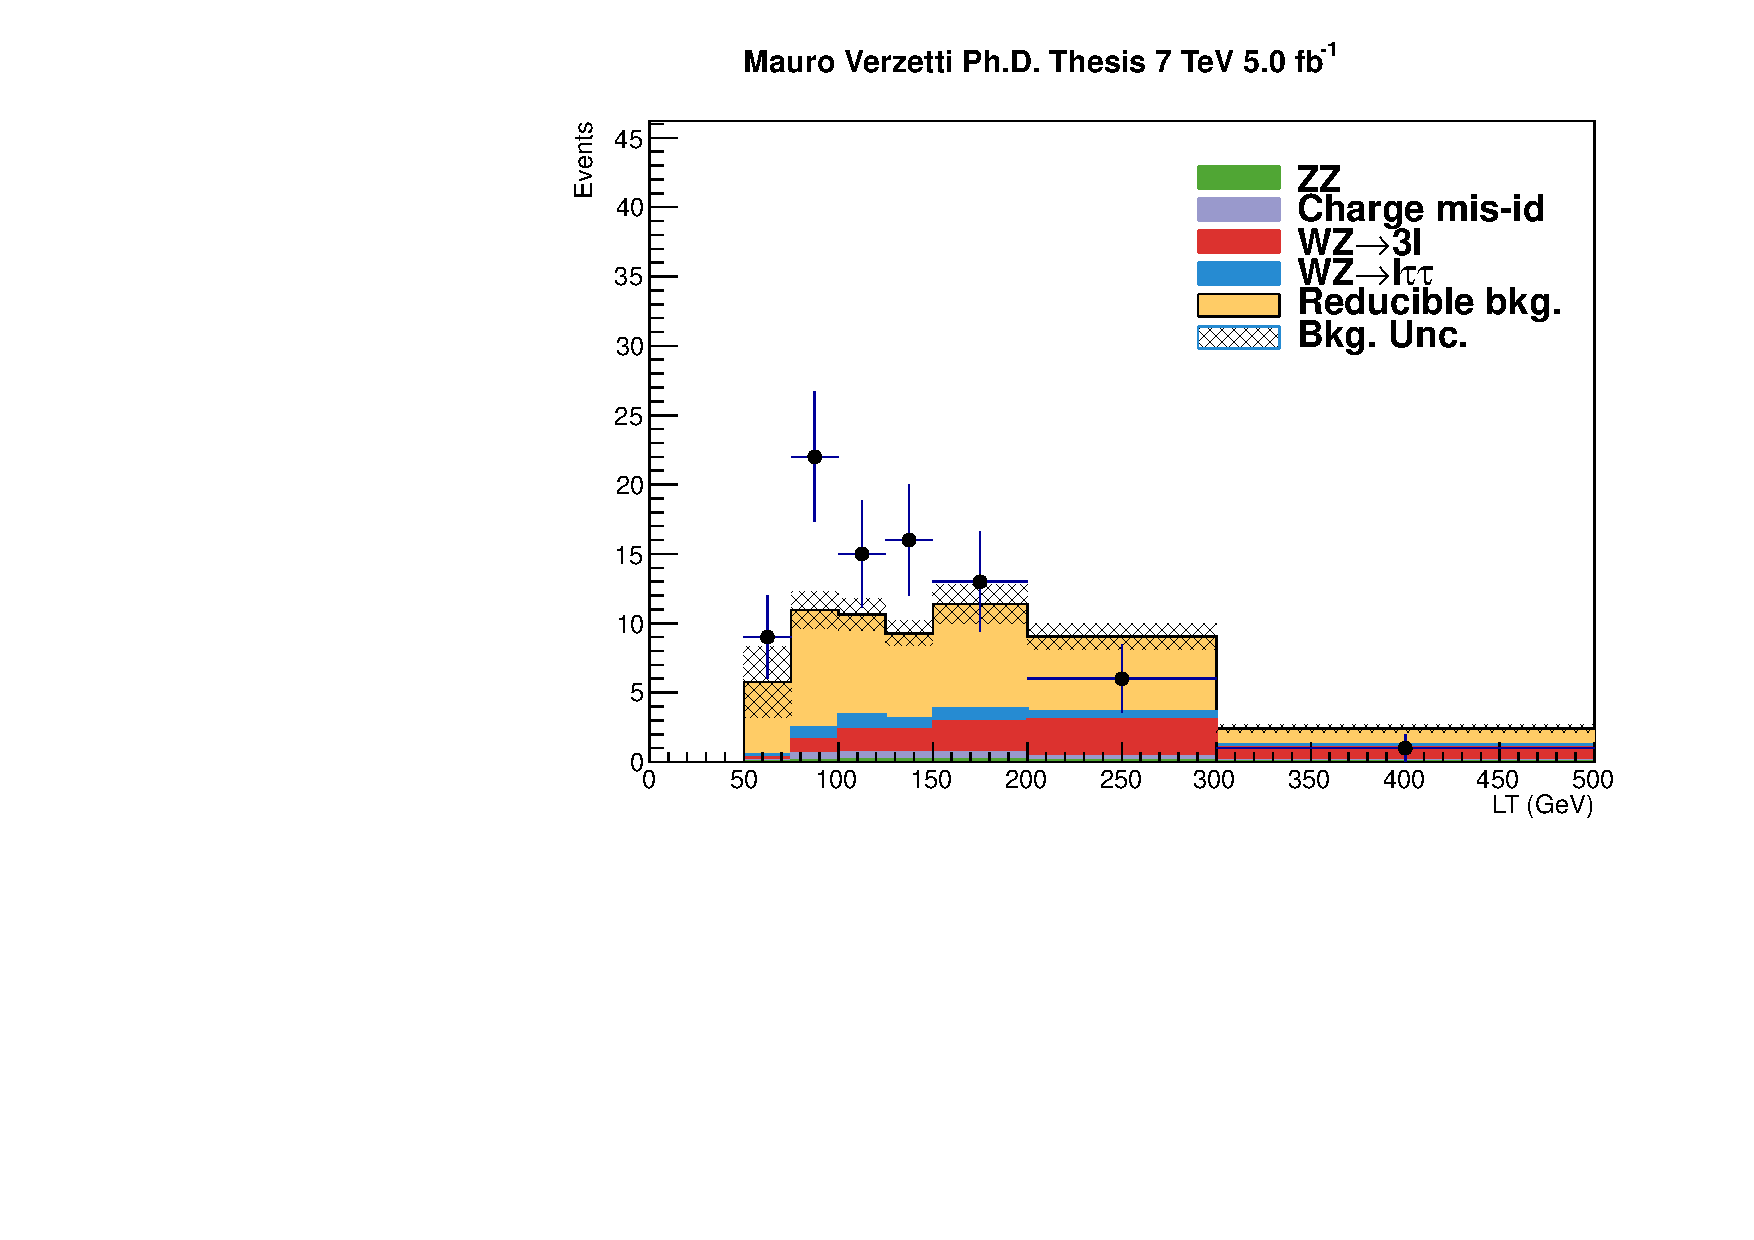
\includegraphics[width=0.49\textwidth]{4_Analisys/pics/7TeV/plots/emt/f3/final-f3-LT.pdf}\\
  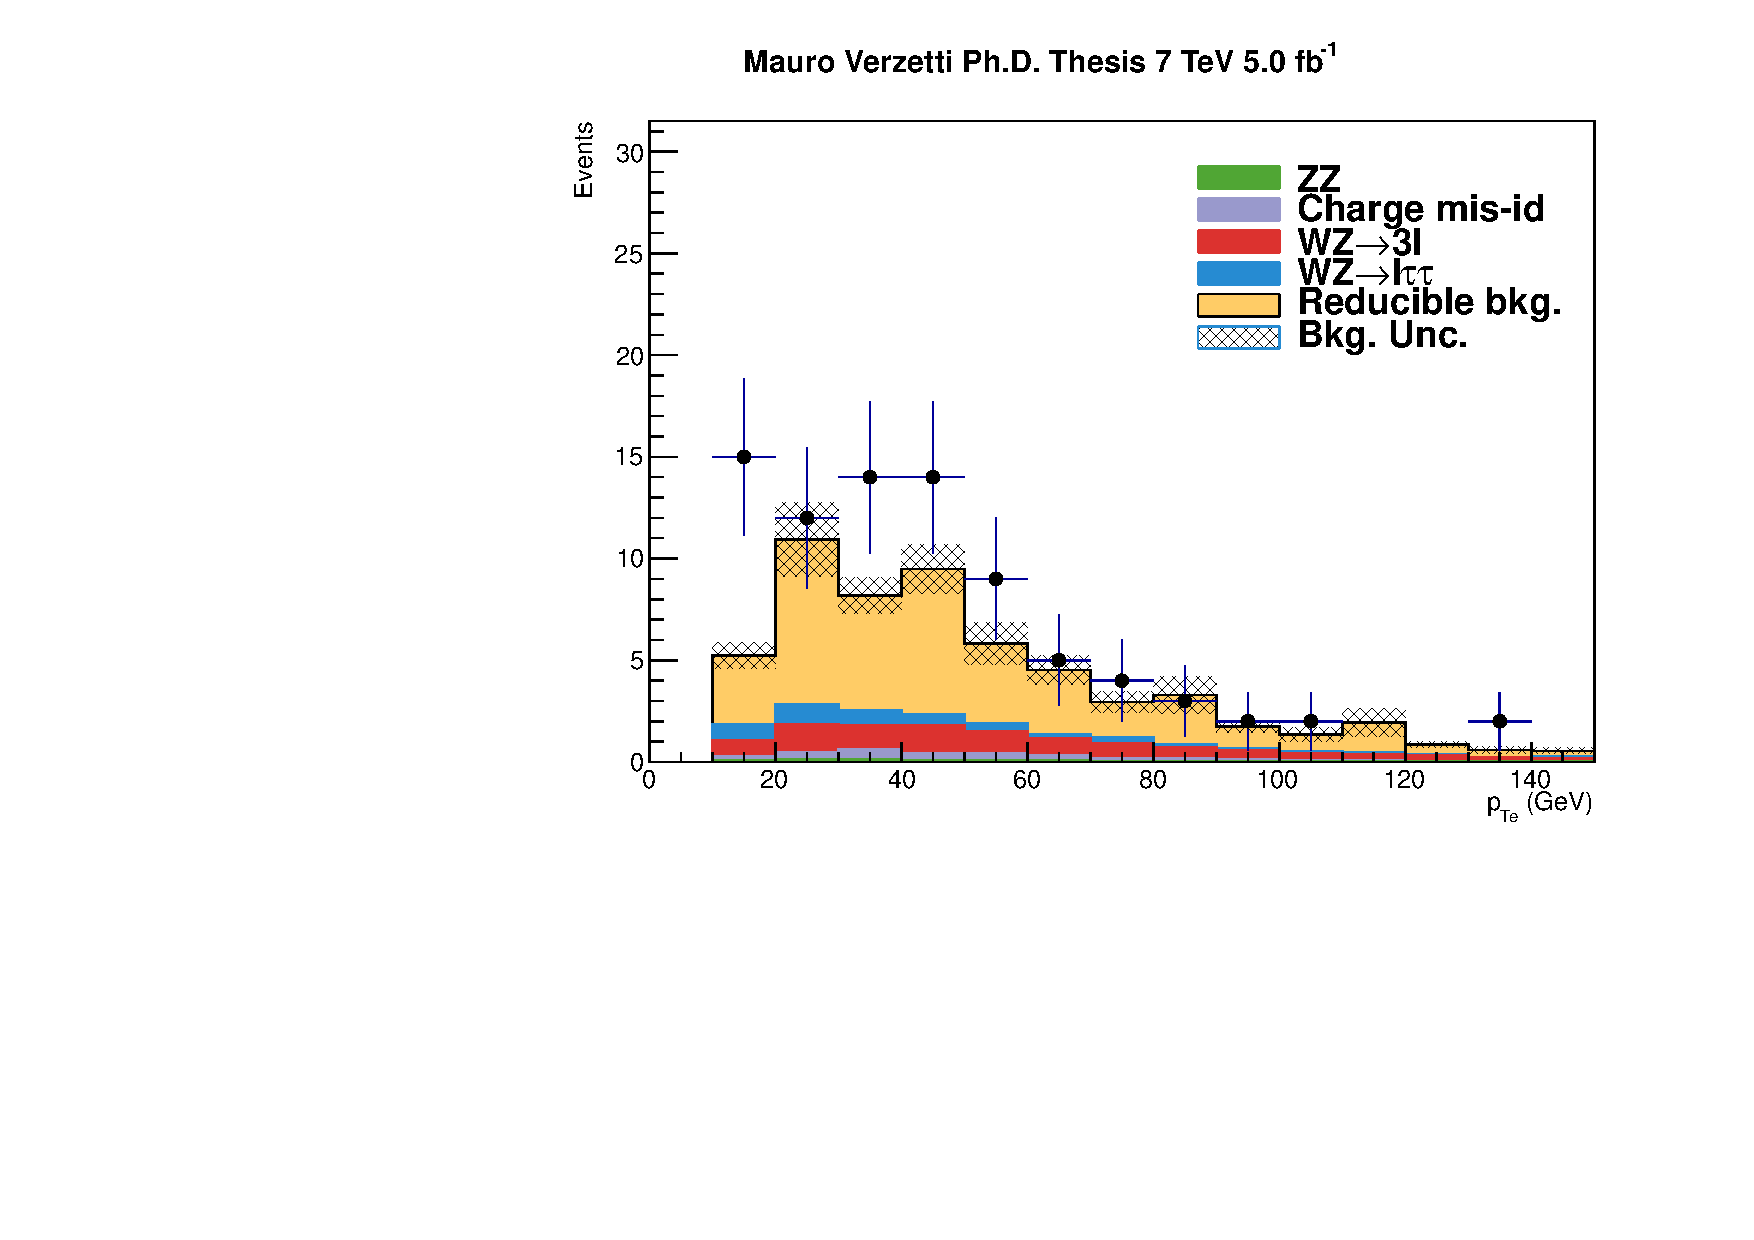
\includegraphics[width=0.49\textwidth]{4_Analisys/pics/7TeV/plots/emt/f3/Full/final-f3-ePt-Full.pdf}
  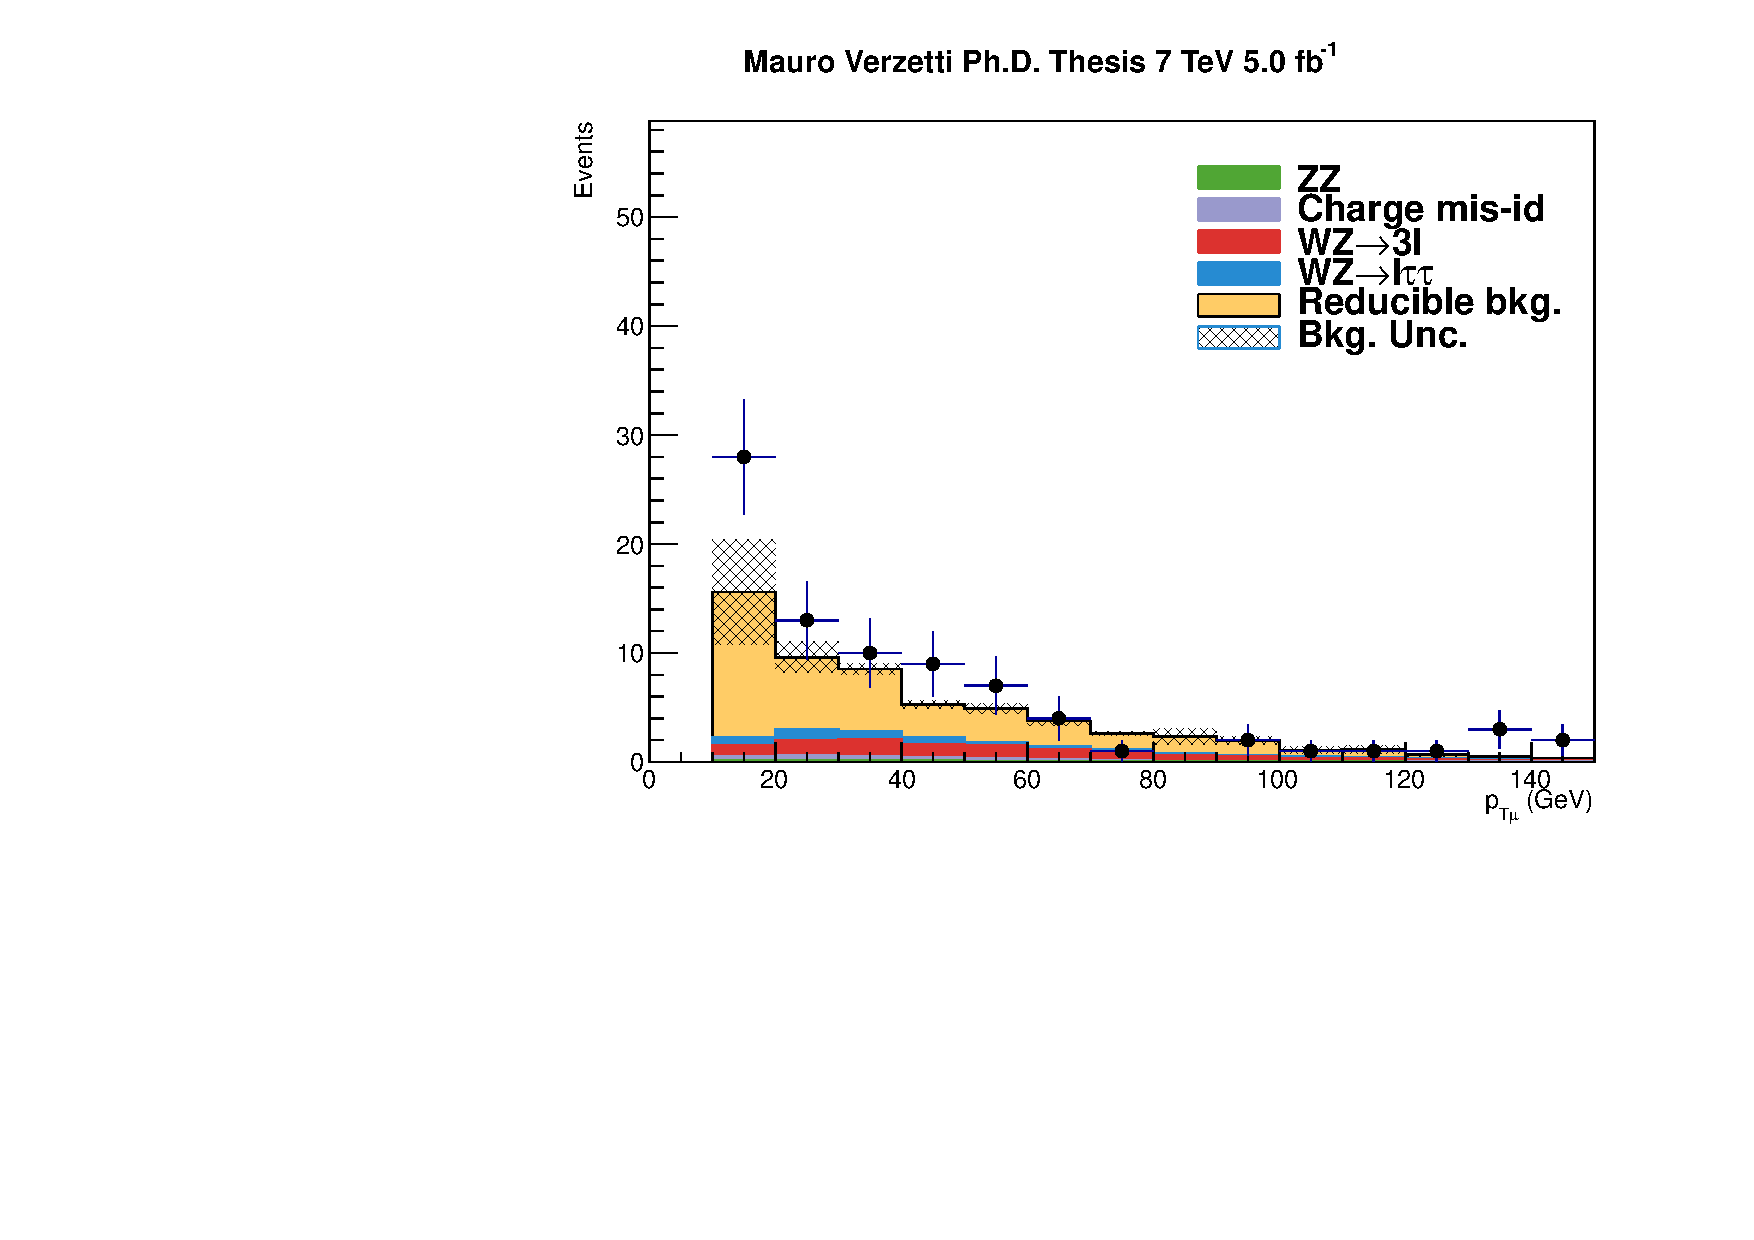
\includegraphics[width=0.49\textwidth]{4_Analisys/pics/7TeV/plots/emt/f3/Full/final-f3-mPt-Full.pdf}\\
  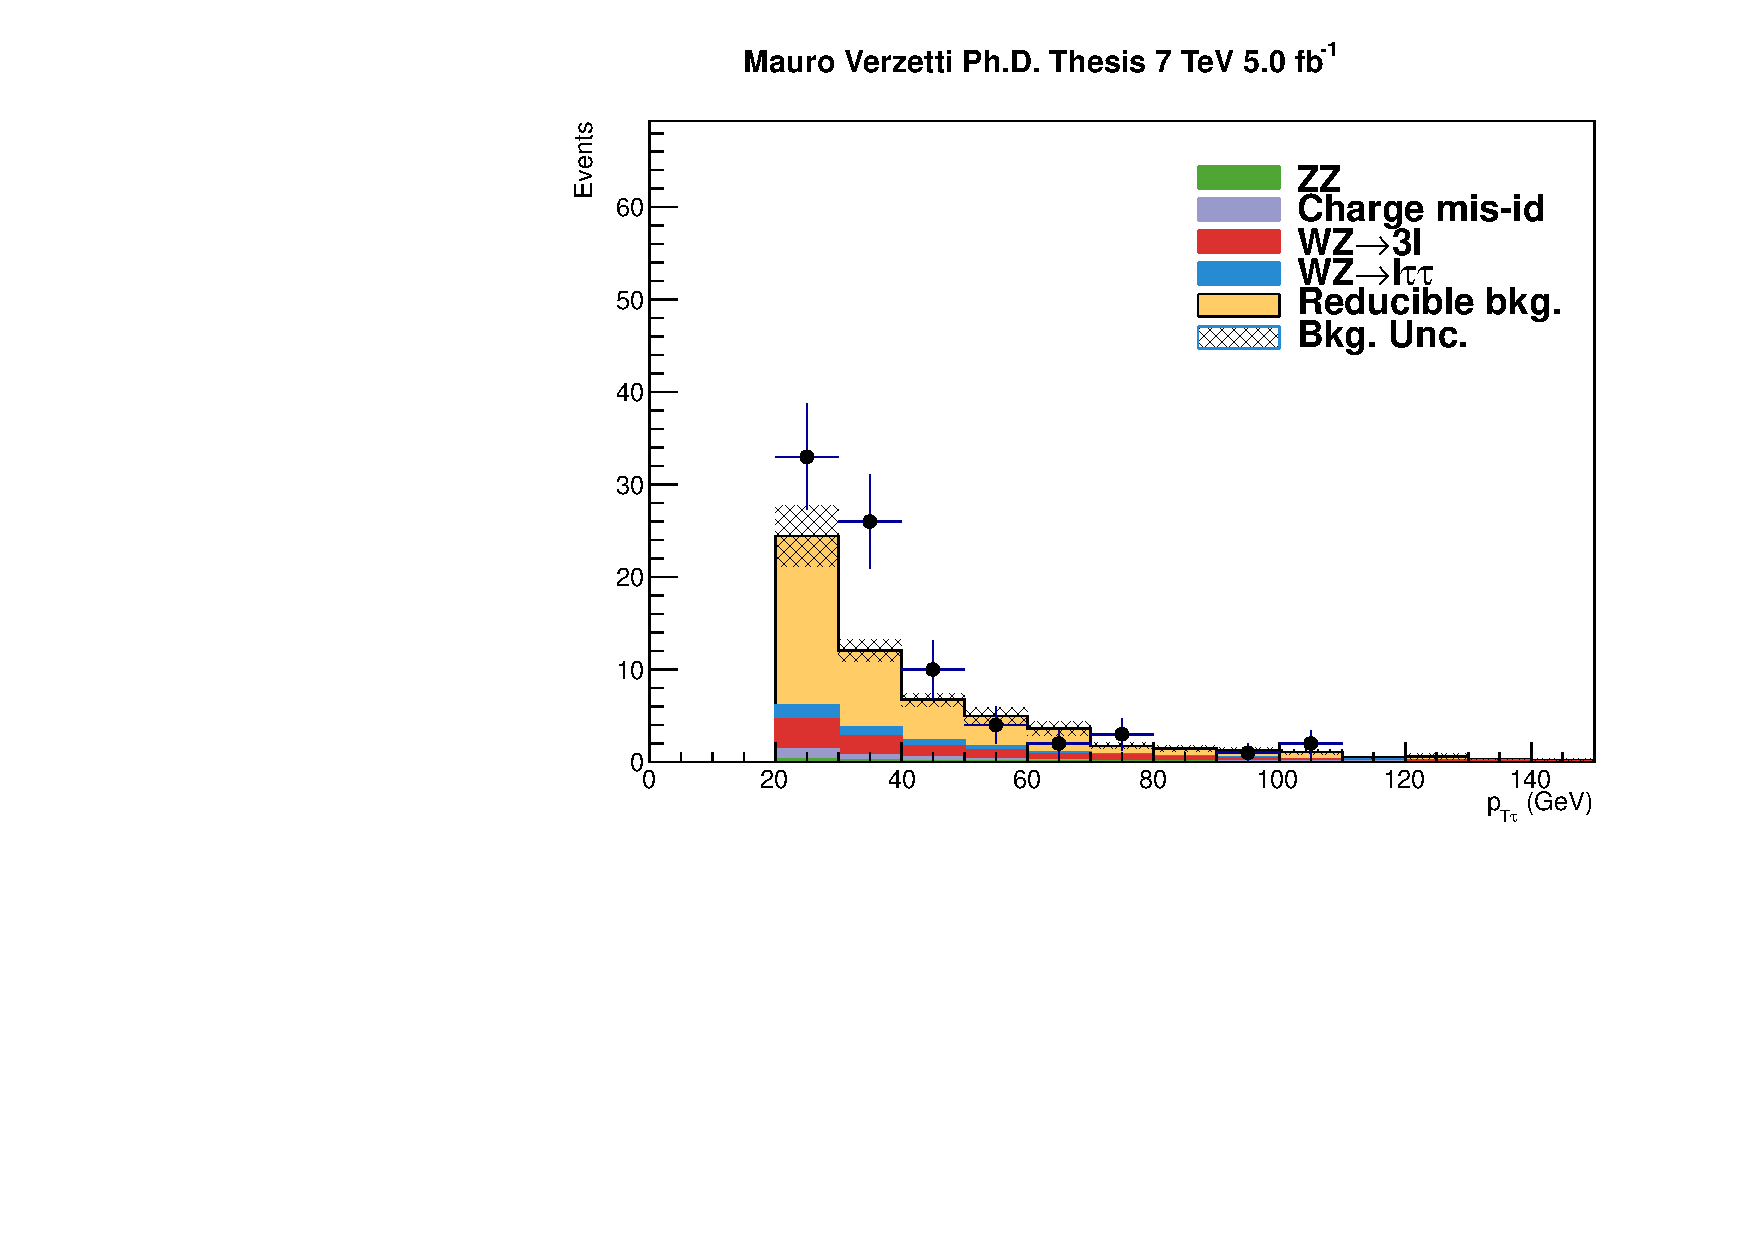
\includegraphics[width=0.49\textwidth]{4_Analisys/pics/7TeV/plots/emt/f3/Full/final-f3-tPt-Full.pdf}
  \caption{Comparison of measured and predicted backgrounds in the $e\mu\tau_h$ ``fake tau'' control region for 7 TeV data.
  From top left to bottom: mass of the sub-leading lepton and the tau system, scalar sum of the leptons \pT ($L_T$), \pT of the electron, muon, and hadronic tau.
  The reducible background contribution is estimated by the kNN method, as in the signal region.
  The shaded band represents the uncertainty on the sum of the background contributions.
  }
  \label{fig:LLT_emt_f3_control_7TeV}
\end{center}
\end{figure}

\begin{figure}
\begin{center}
  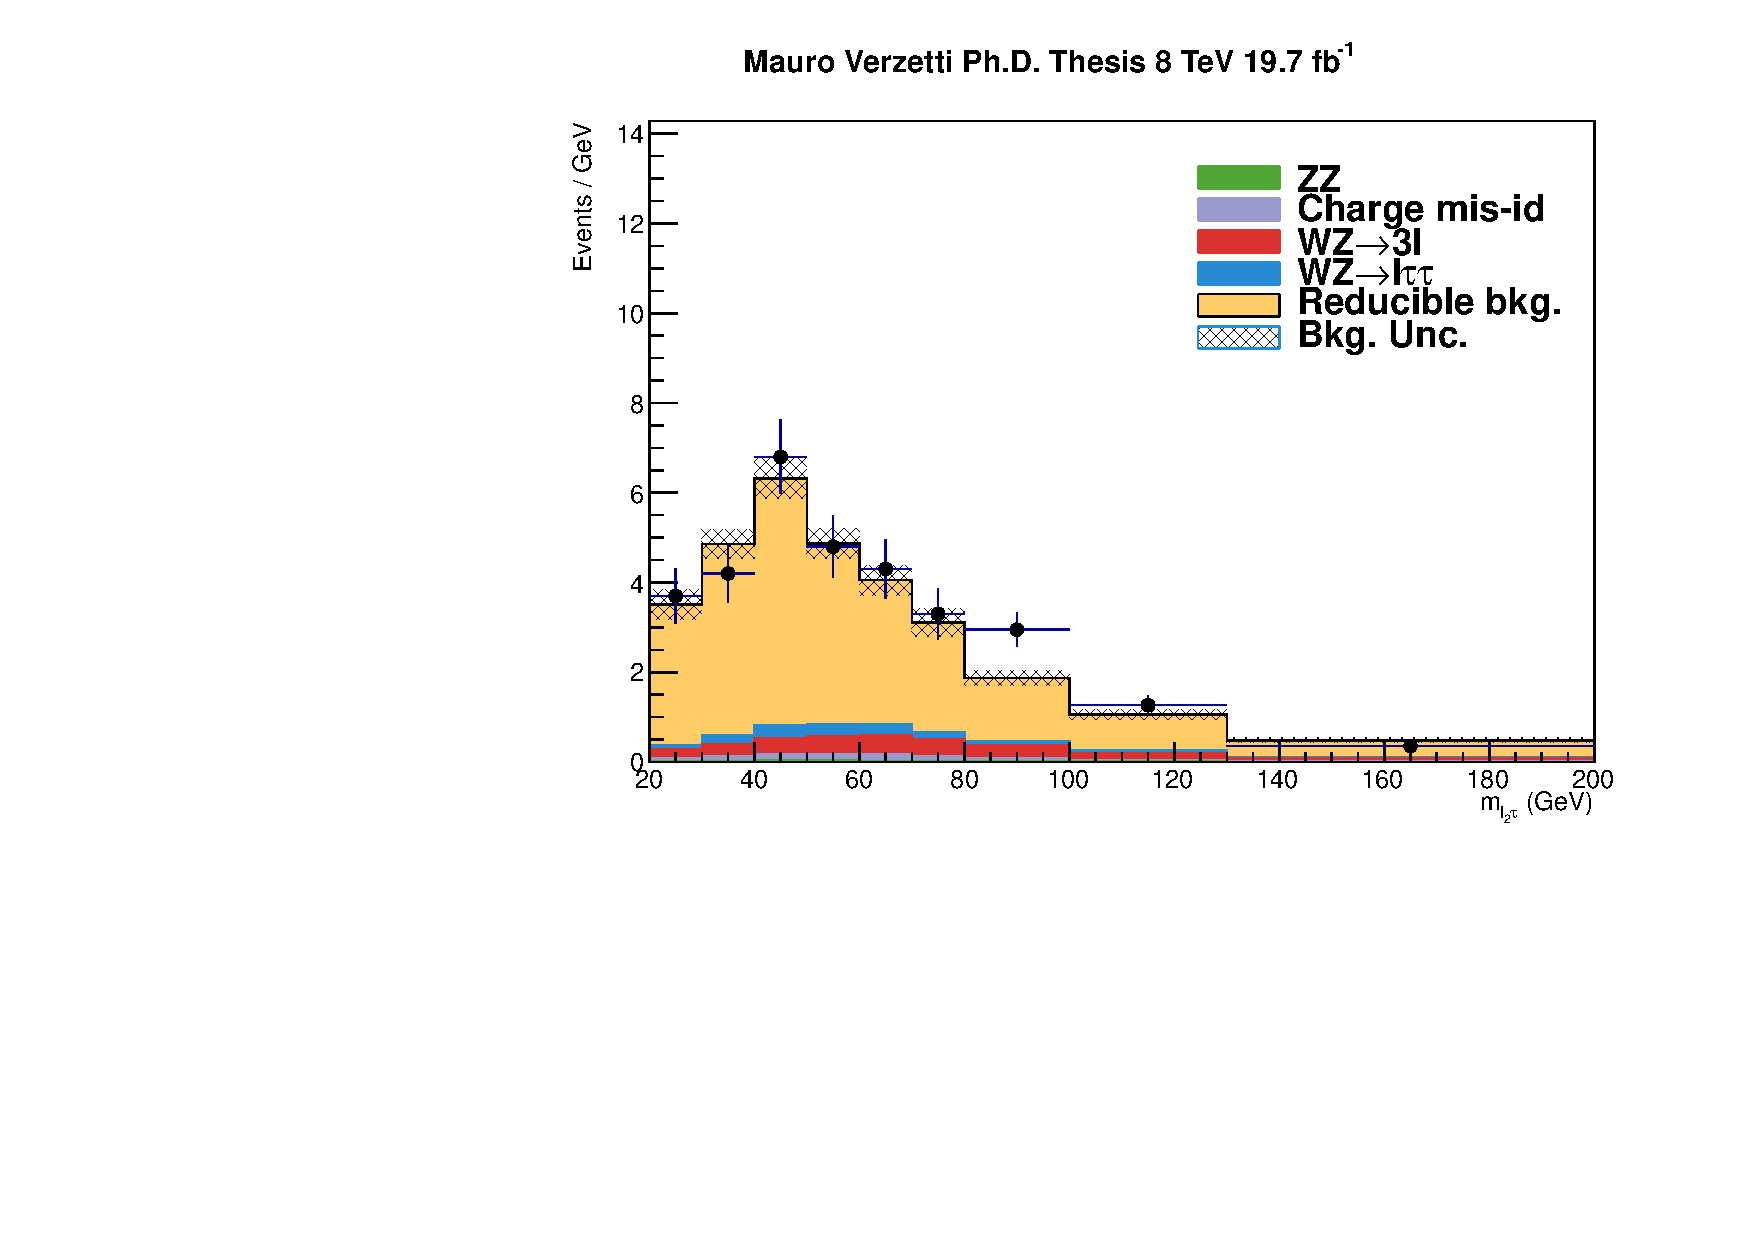
\includegraphics[width=0.49\textwidth]{4_Analisys/pics/8TeV/plots/emt/f3/Full/final-f3-subMass-Full.pdf}
  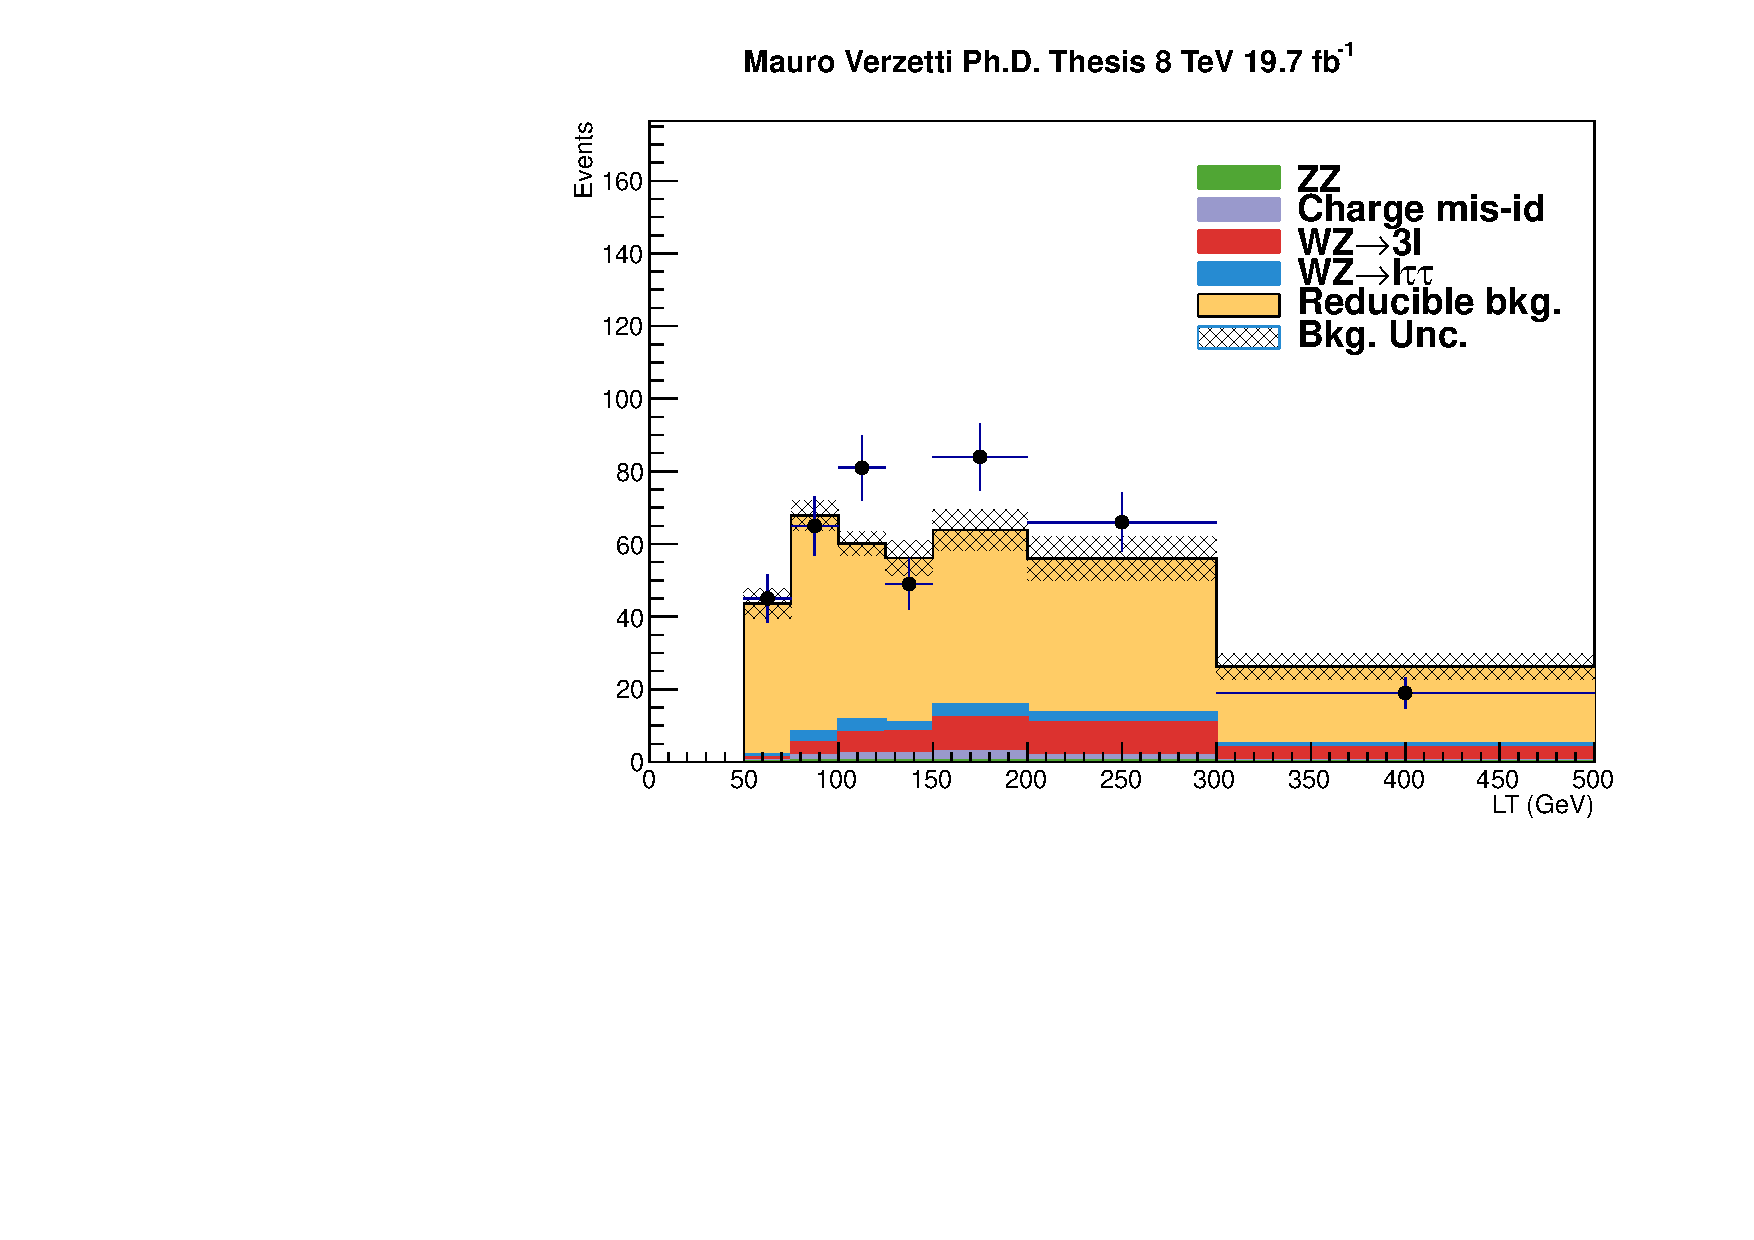
\includegraphics[width=0.49\textwidth]{4_Analisys/pics/8TeV/plots/emt/f3/final-f3-LT.pdf}\\
  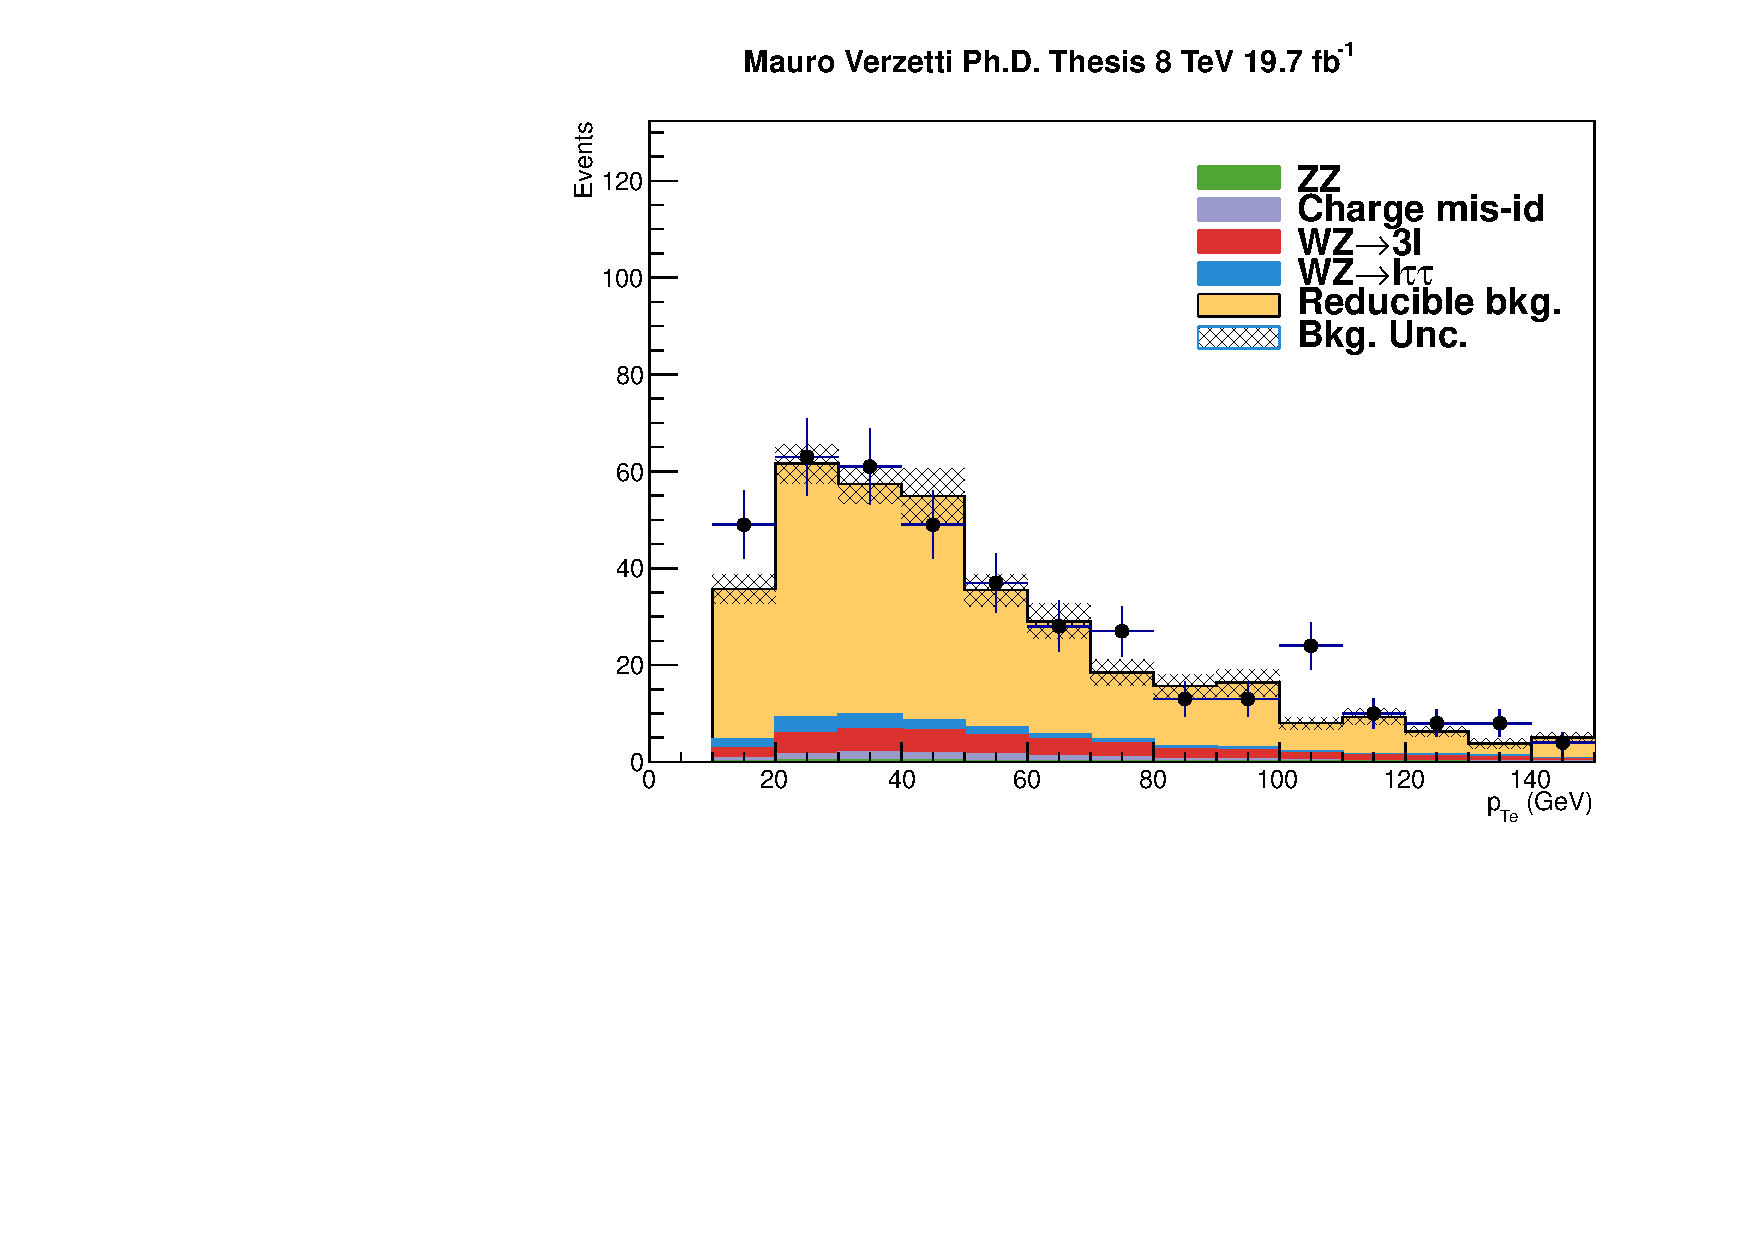
\includegraphics[width=0.49\textwidth]{4_Analisys/pics/8TeV/plots/emt/f3/Full/final-f3-ePt-Full.pdf}
  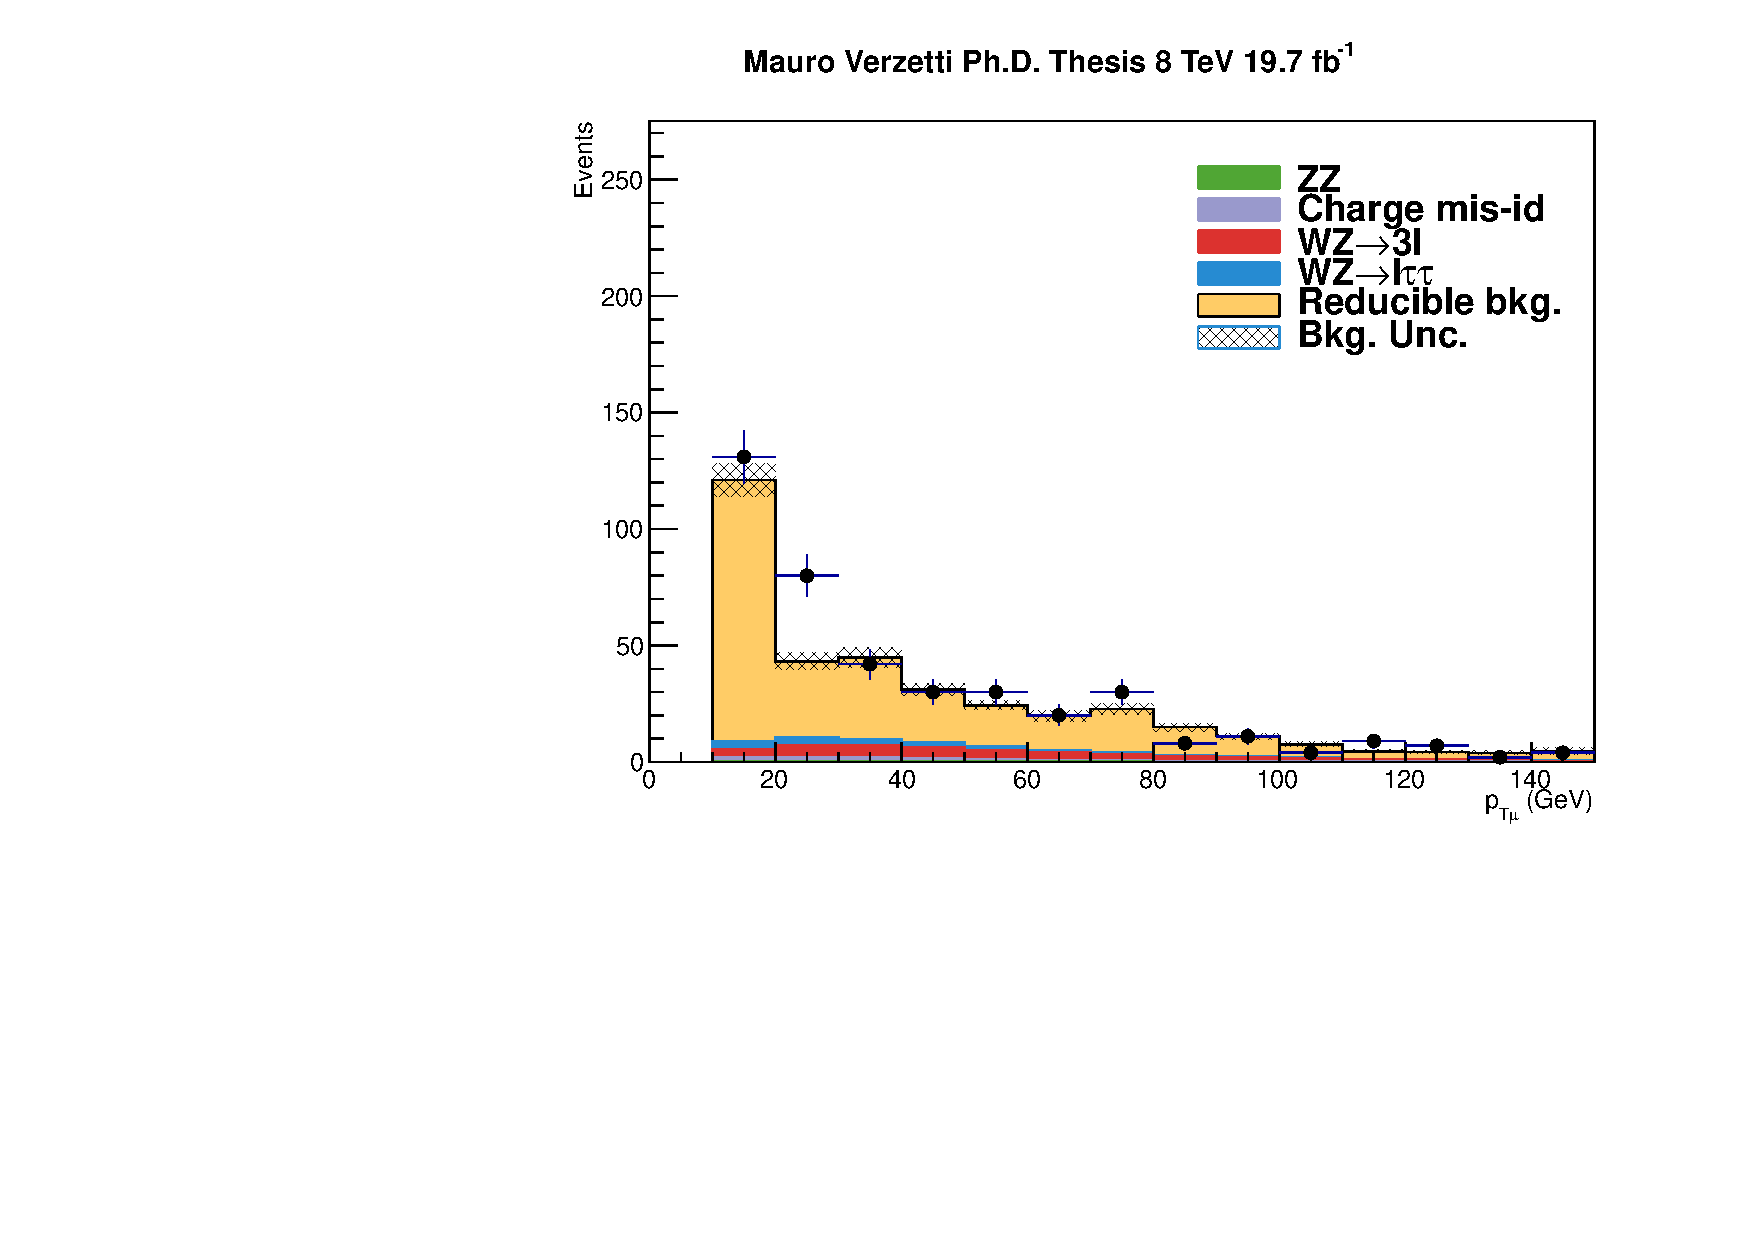
\includegraphics[width=0.49\textwidth]{4_Analisys/pics/8TeV/plots/emt/f3/Full/final-f3-mPt-Full.pdf}\\
  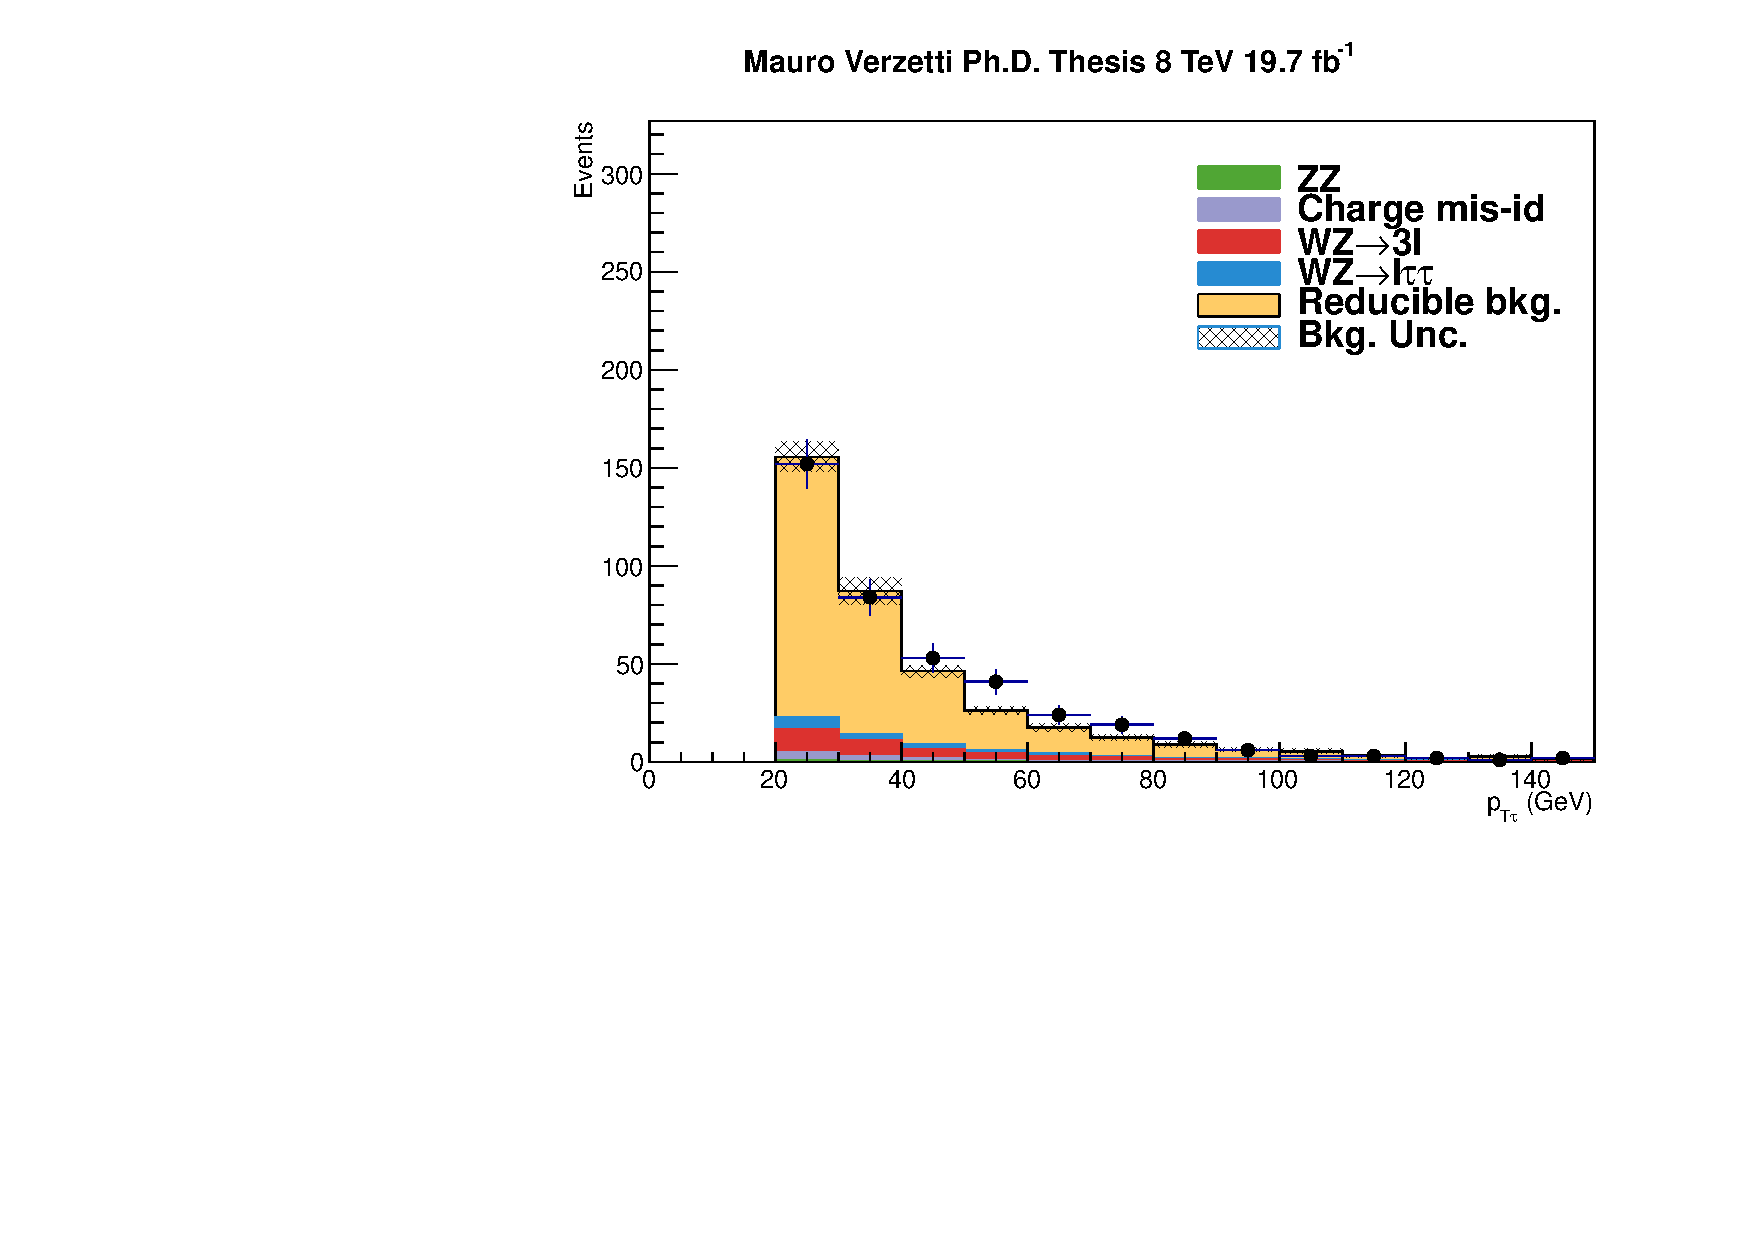
\includegraphics[width=0.49\textwidth]{4_Analisys/pics/8TeV/plots/emt/f3/Full/final-f3-tPt-Full.pdf}
  \caption{Comparison of measured and predicted backgrounds in the $e\mu\tau_h$ ``fake tau'' control region for 8 TeV data.
  From top left to bottom: mass of the sub-leading lepton and the tau system, scalar sum of the leptons \pT ($L_T$), \pT of the electron, muon, and hadronic tau.
  The reducible background contribution is estimated by the kNN method, as in the signal region.
  The shaded band represents the uncertainty on the sum of the background contributions.
  }
  \label{fig:LLT_emt_f3_control_8TeV}
\end{center}
\end{figure}


\begin{figure}
\begin{center}
  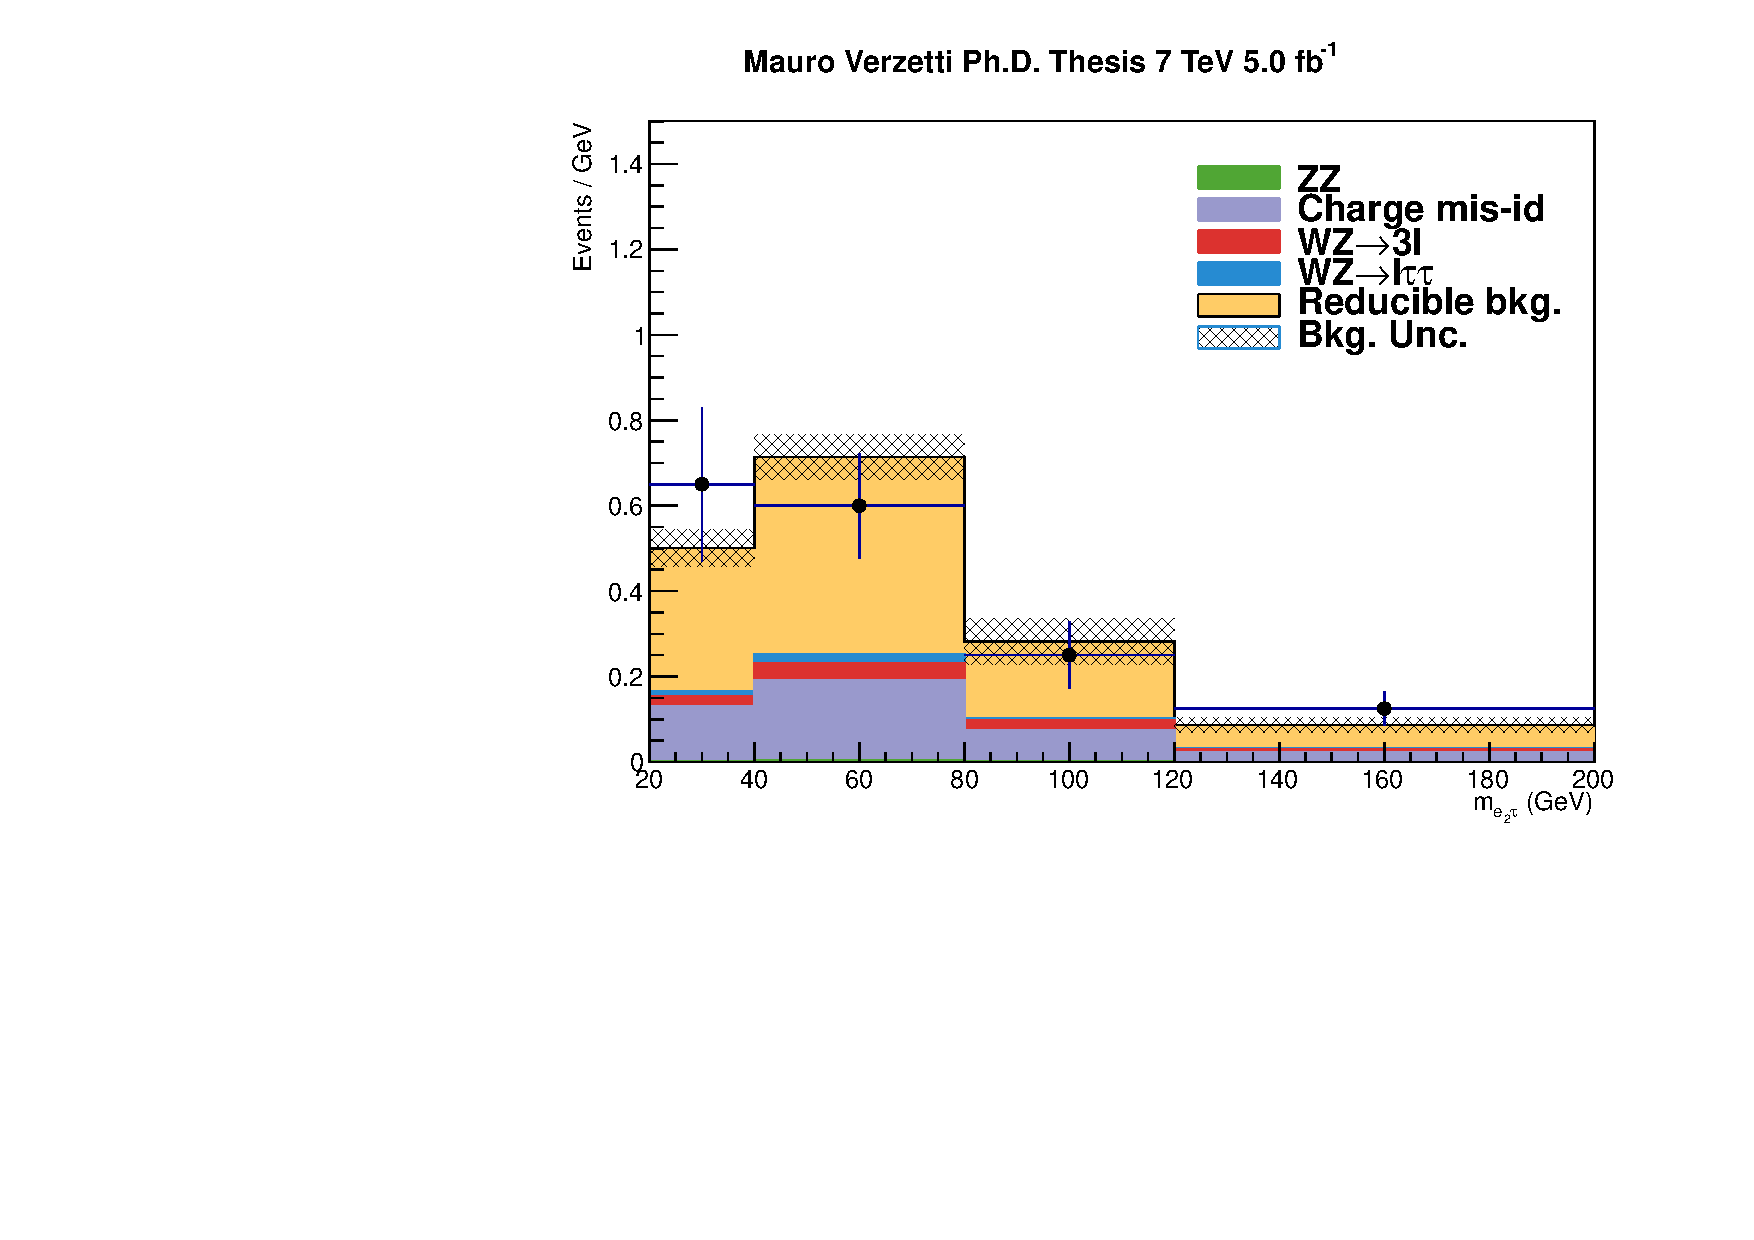
\includegraphics[width=0.49\textwidth]{4_Analisys/pics/7TeV/plots/eet/f3/Full/final-f3-subMass-Full.pdf}
  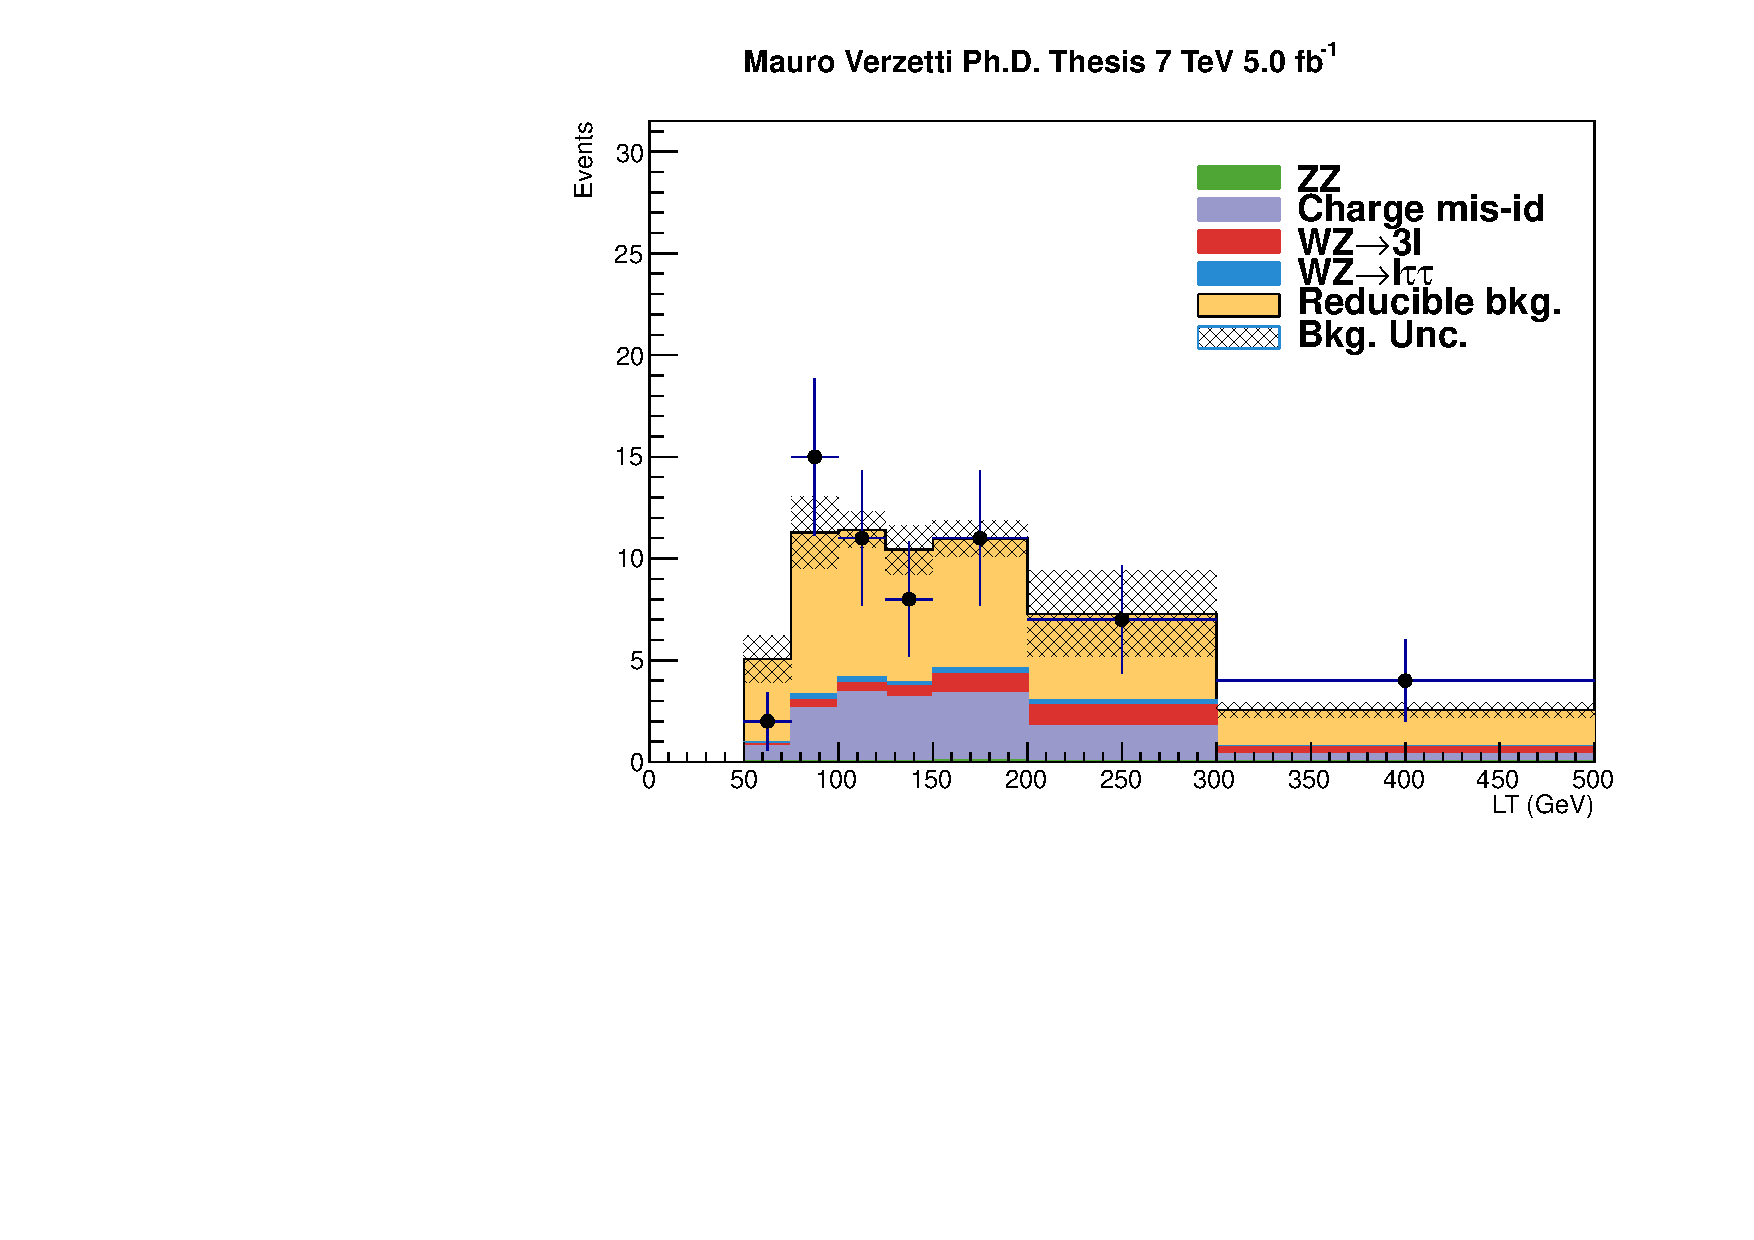
\includegraphics[width=0.49\textwidth]{4_Analisys/pics/7TeV/plots/eet/f3/final-f3-LT.pdf}\\
  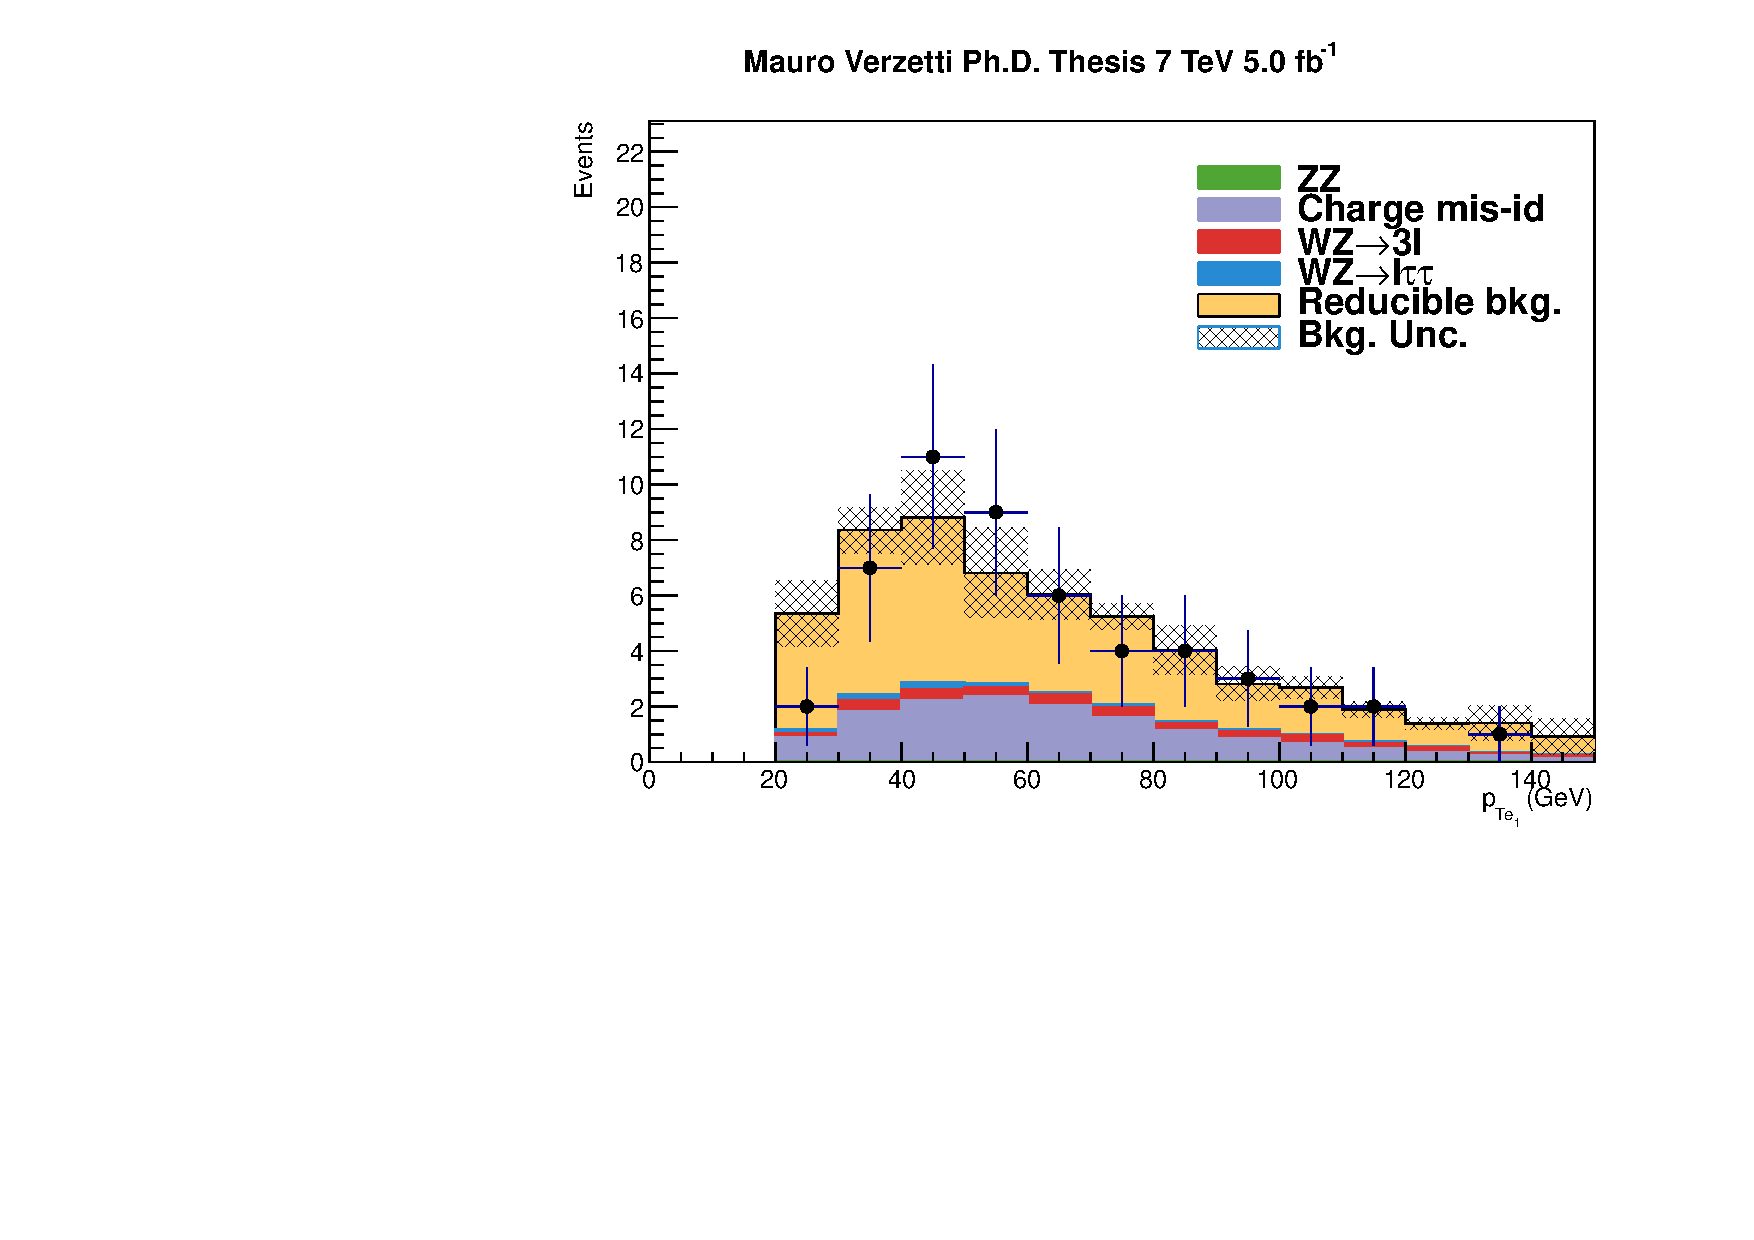
\includegraphics[width=0.49\textwidth]{4_Analisys/pics/7TeV/plots/eet/f3/Full/final-f3-e1Pt-Full.pdf}
  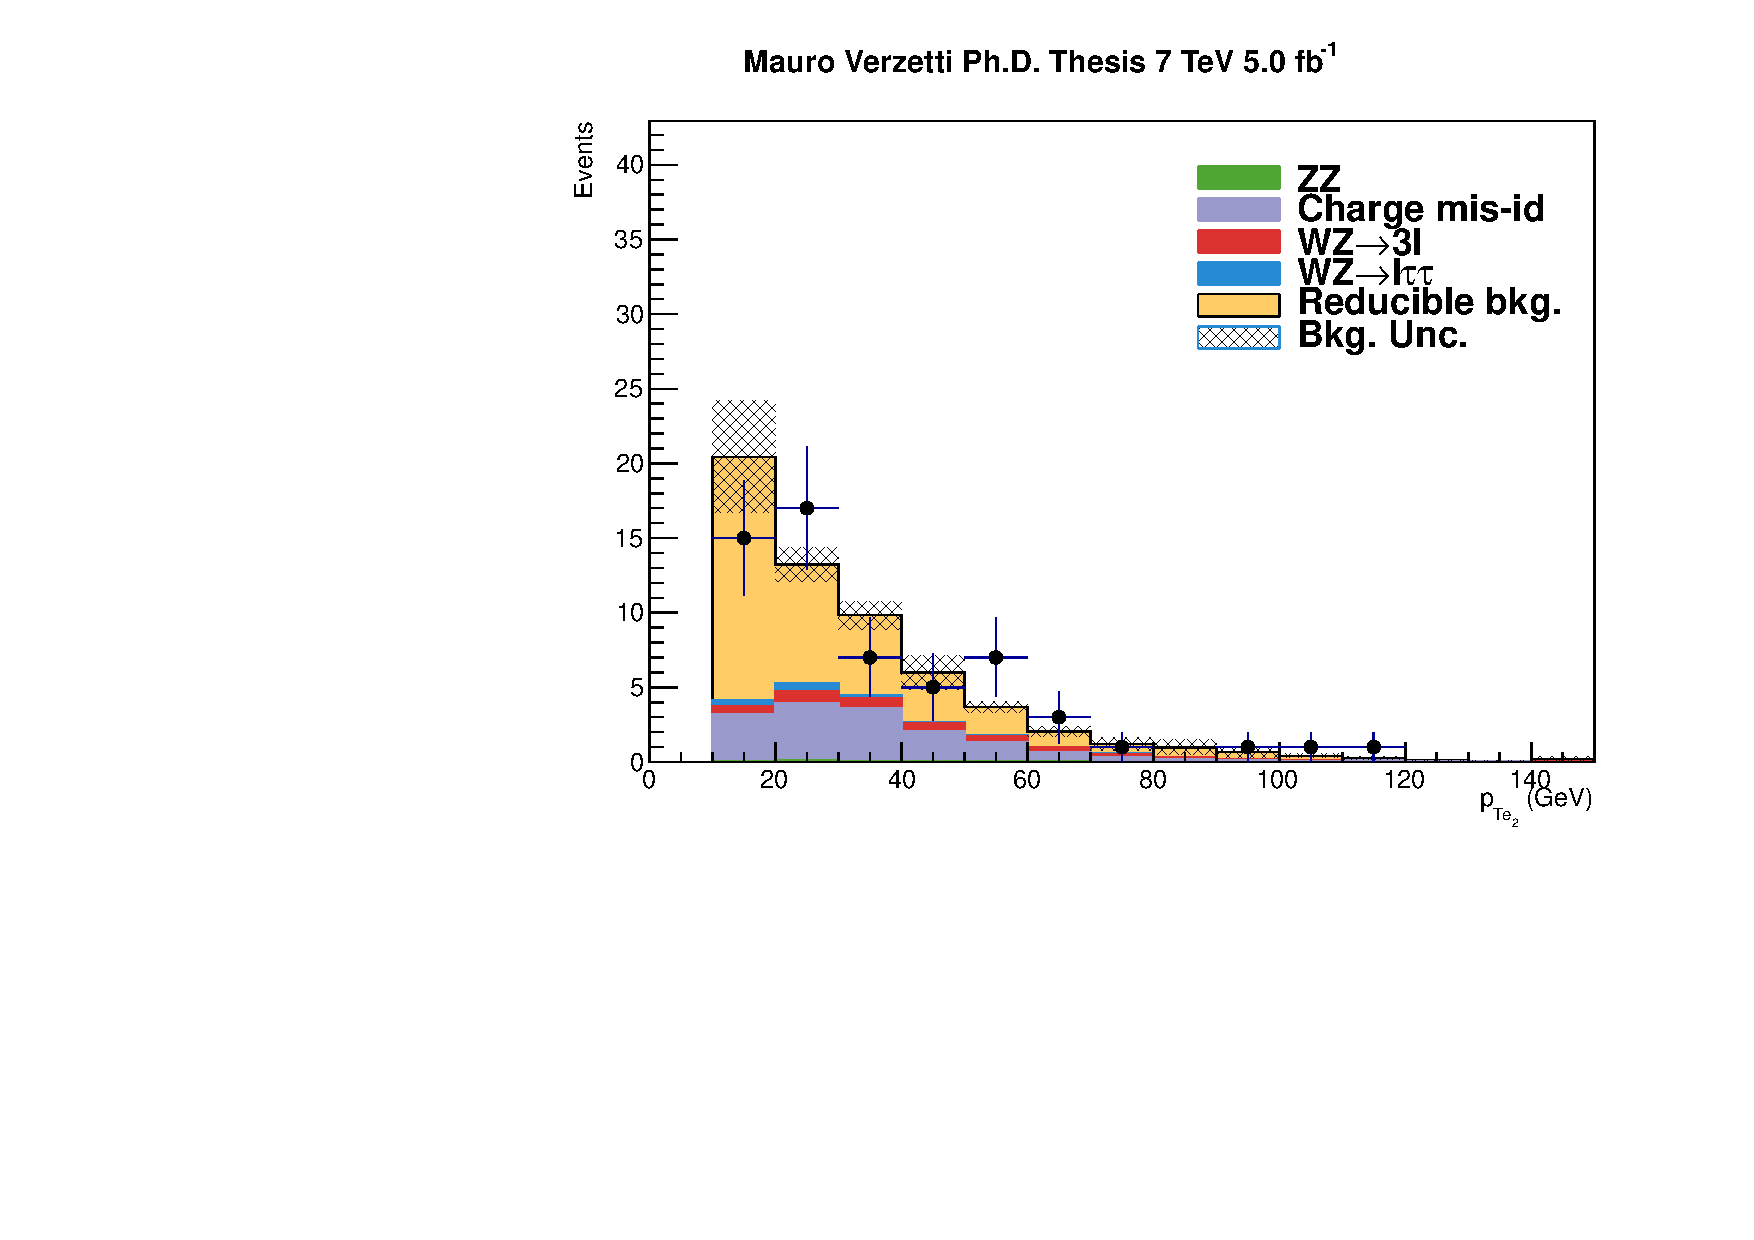
\includegraphics[width=0.49\textwidth]{4_Analisys/pics/7TeV/plots/eet/f3/Full/final-f3-e2Pt-Full.pdf}\\
  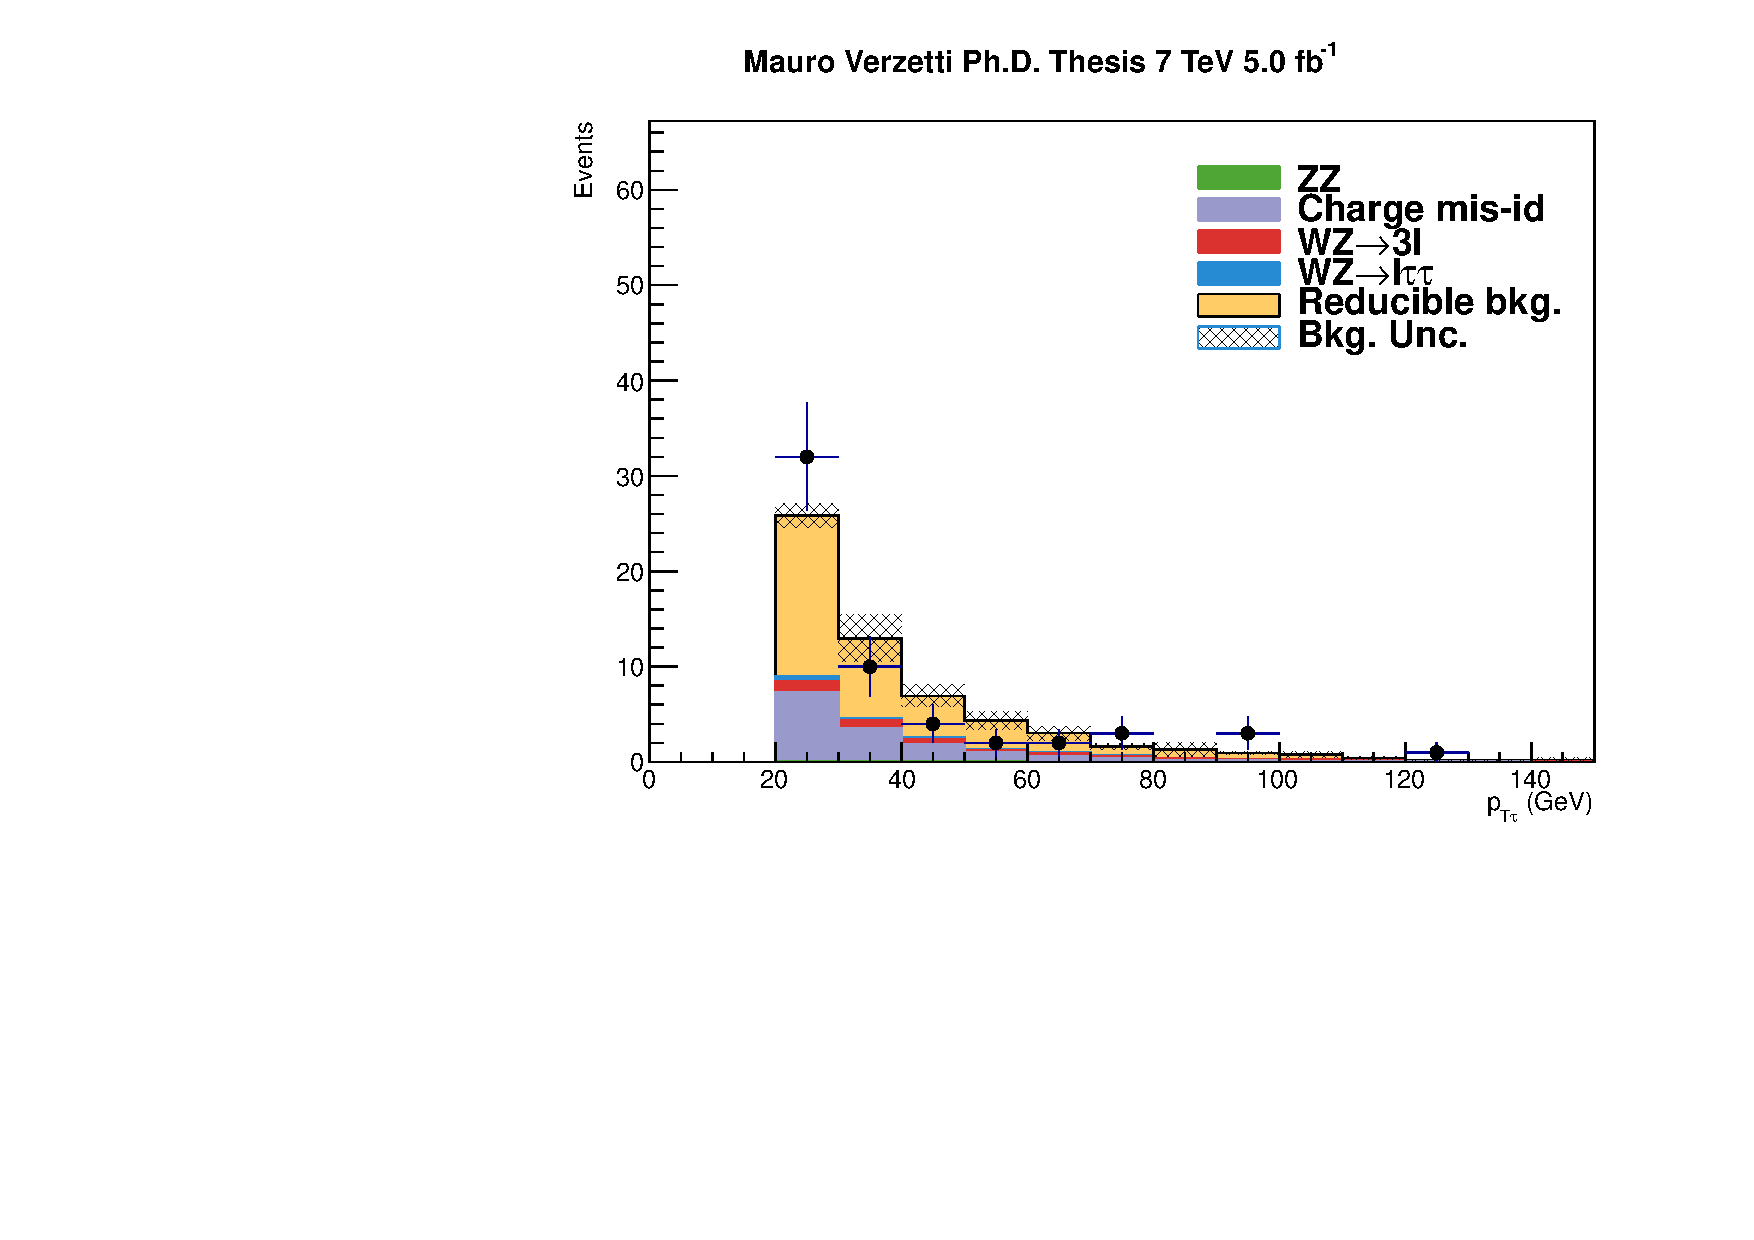
\includegraphics[width=0.49\textwidth]{4_Analisys/pics/7TeV/plots/eet/f3/Full/final-f3-tPt-Full.pdf}
  \caption{Comparison of measured and predicted backgrounds in the $ee\tau_h$ ``fake tau'' control region for 7 TeV data.
  From top left to bottom: mass of the sub-leading electron and the tau system, scalar sum of the leptons \pT ($L_T$), \pT of the leading and sub-leading electron, and \pT of the hadronic tau.
  The reducible background contribution is estimated by the kNN method, as in the signal region.
  The shaded band represents the uncertainty on the sum of the background contributions.
  }
  \label{fig:LLT_eet_f3_control_7TeV}
\end{center}
\end{figure}

\begin{figure}
\begin{center}
  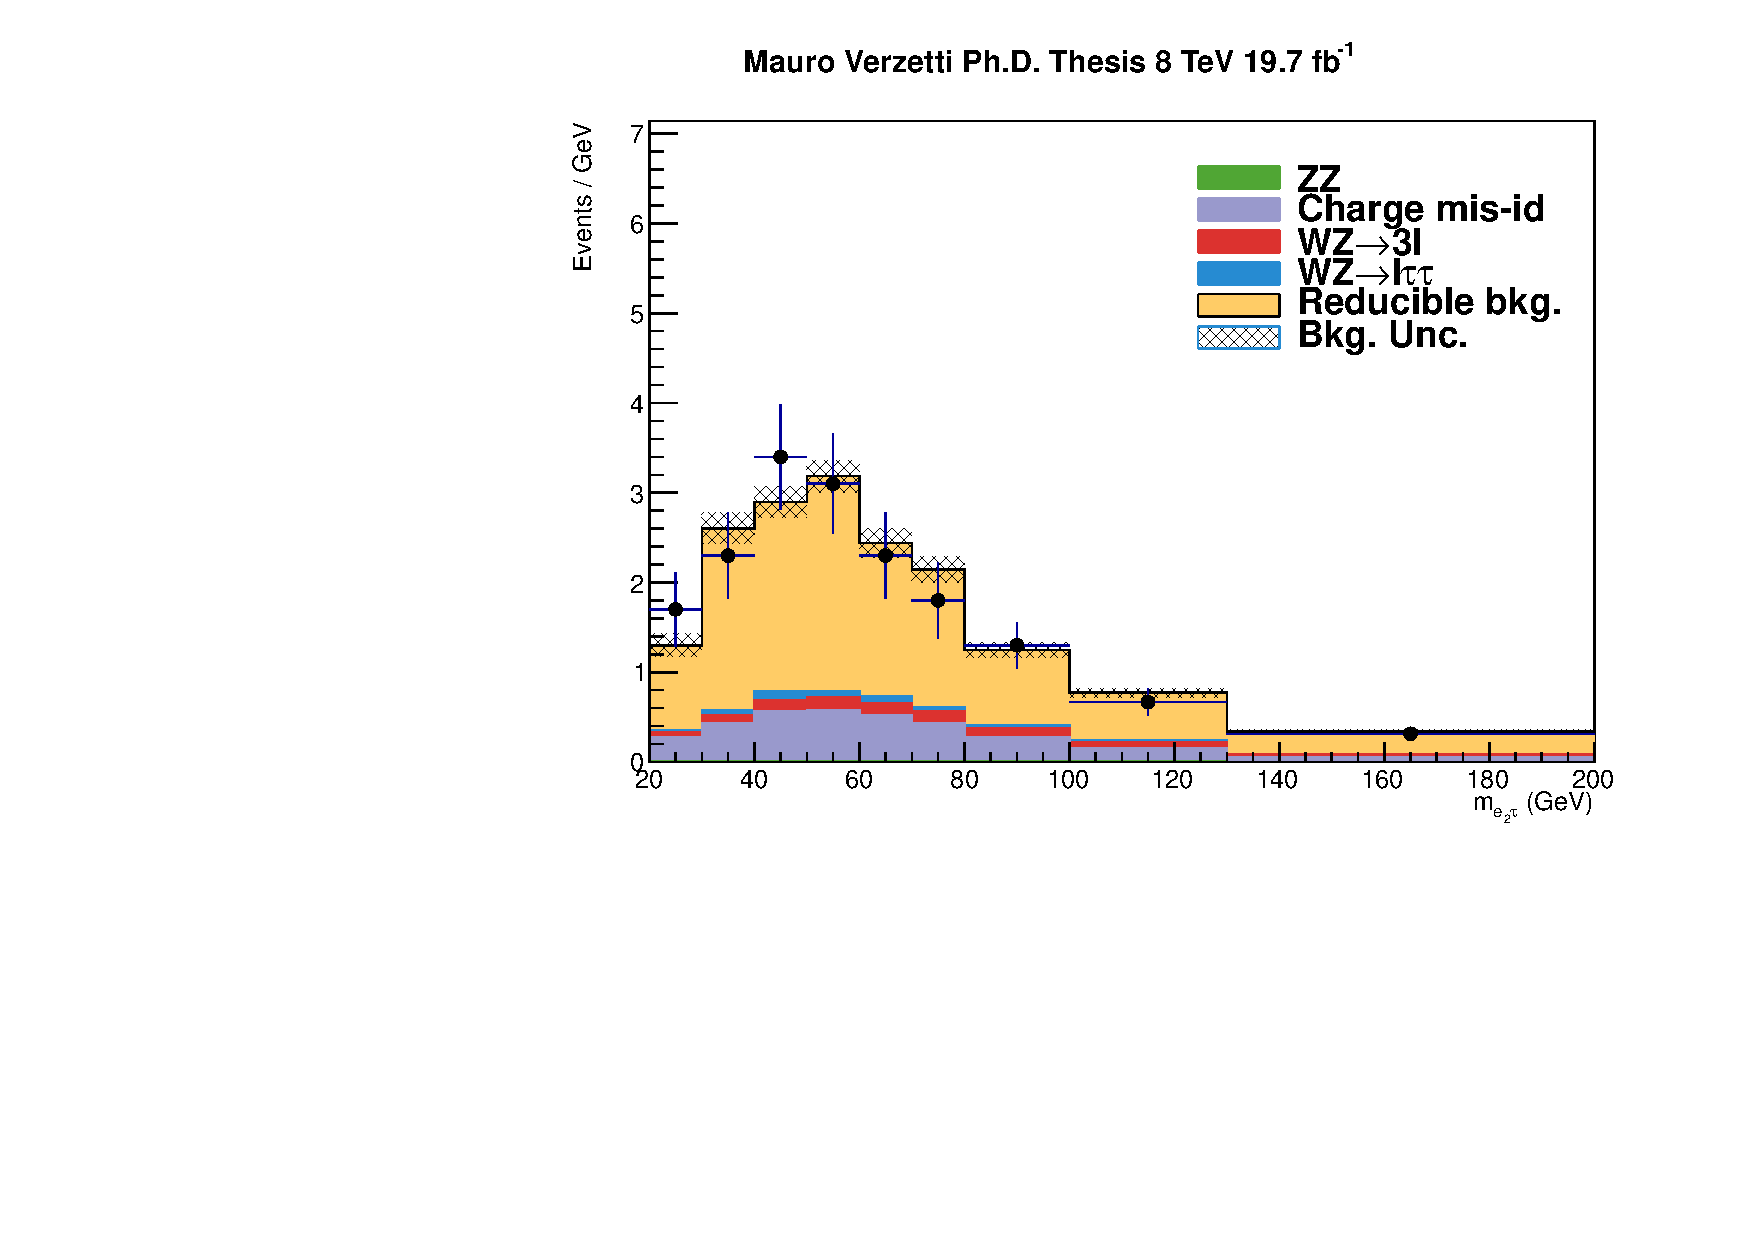
\includegraphics[width=0.49\textwidth]{4_Analisys/pics/8TeV/plots/eet/f3/Full/final-f3-subMass-Full.pdf}
  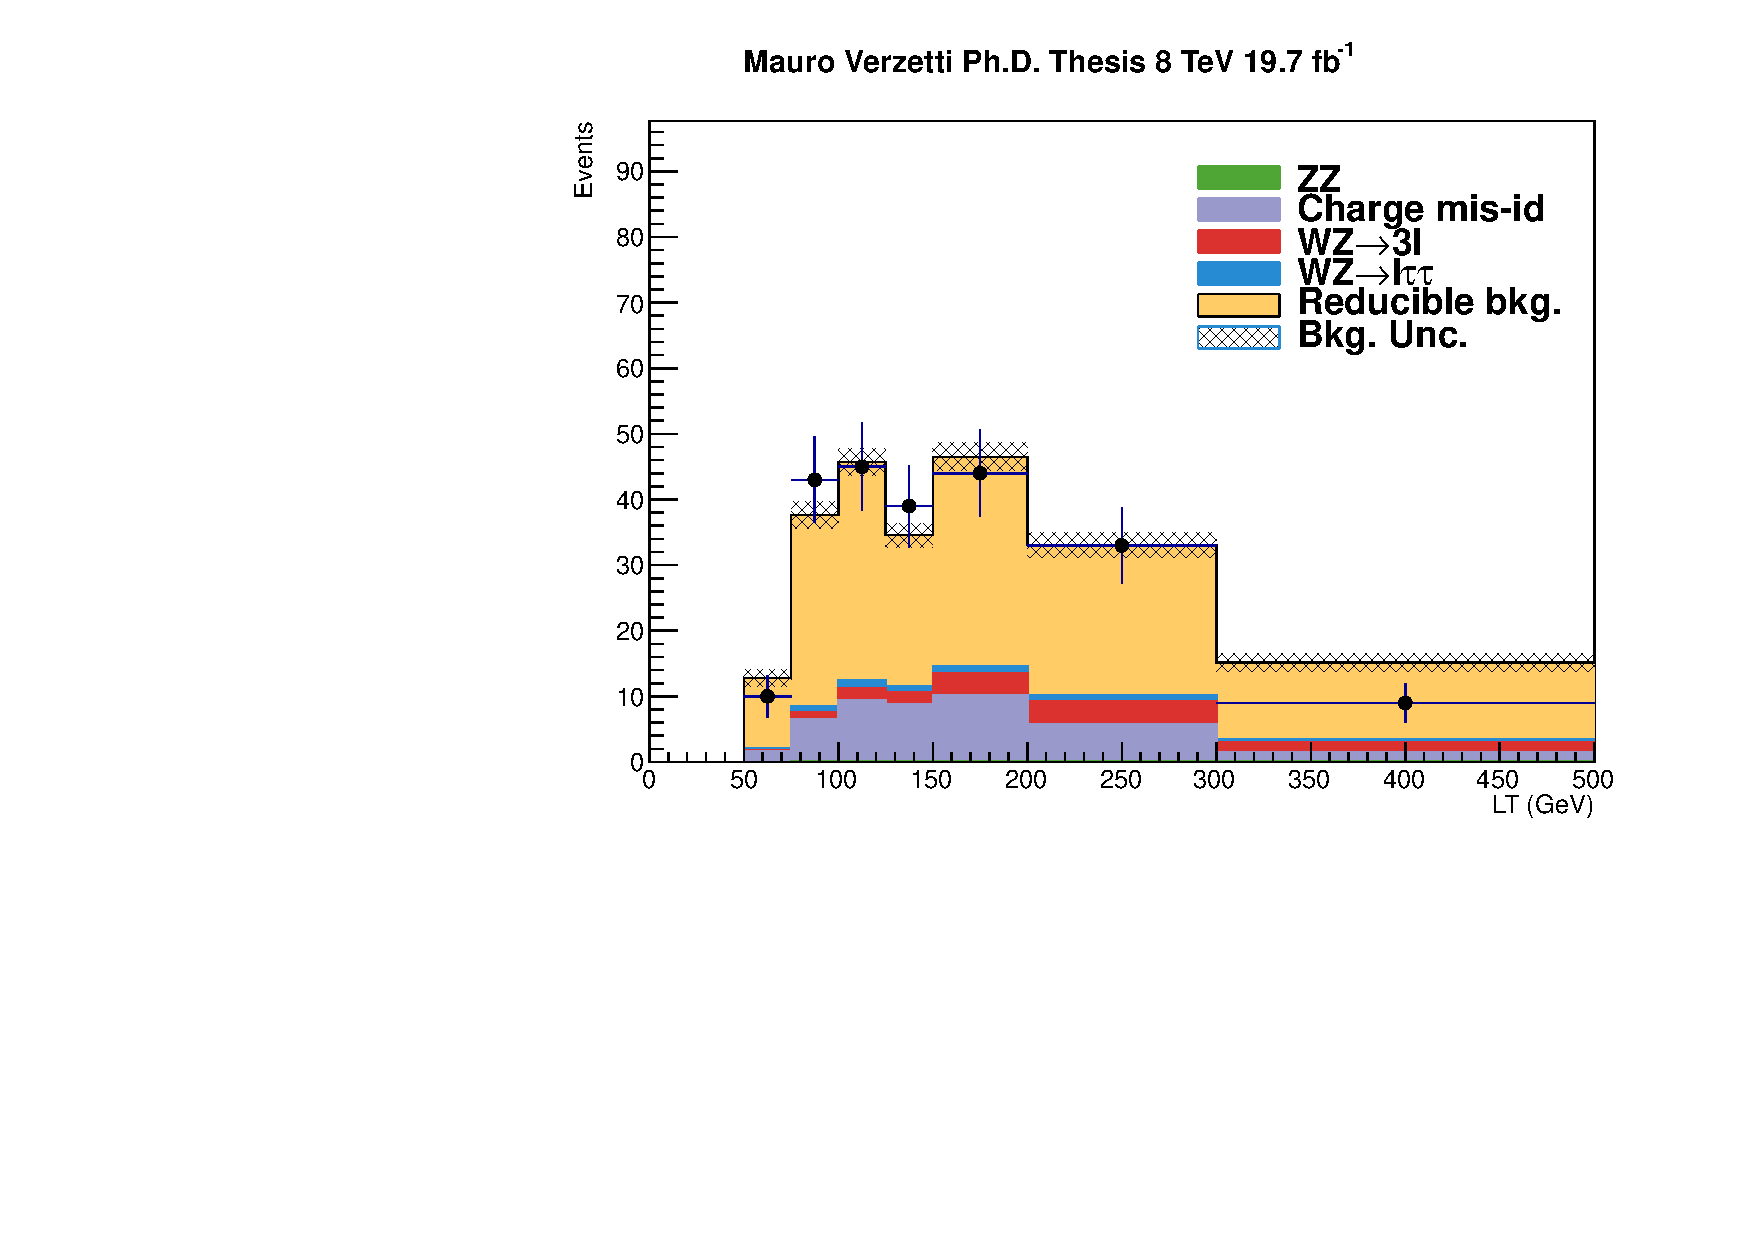
\includegraphics[width=0.49\textwidth]{4_Analisys/pics/8TeV/plots/eet/f3/final-f3-LT.pdf}\\
  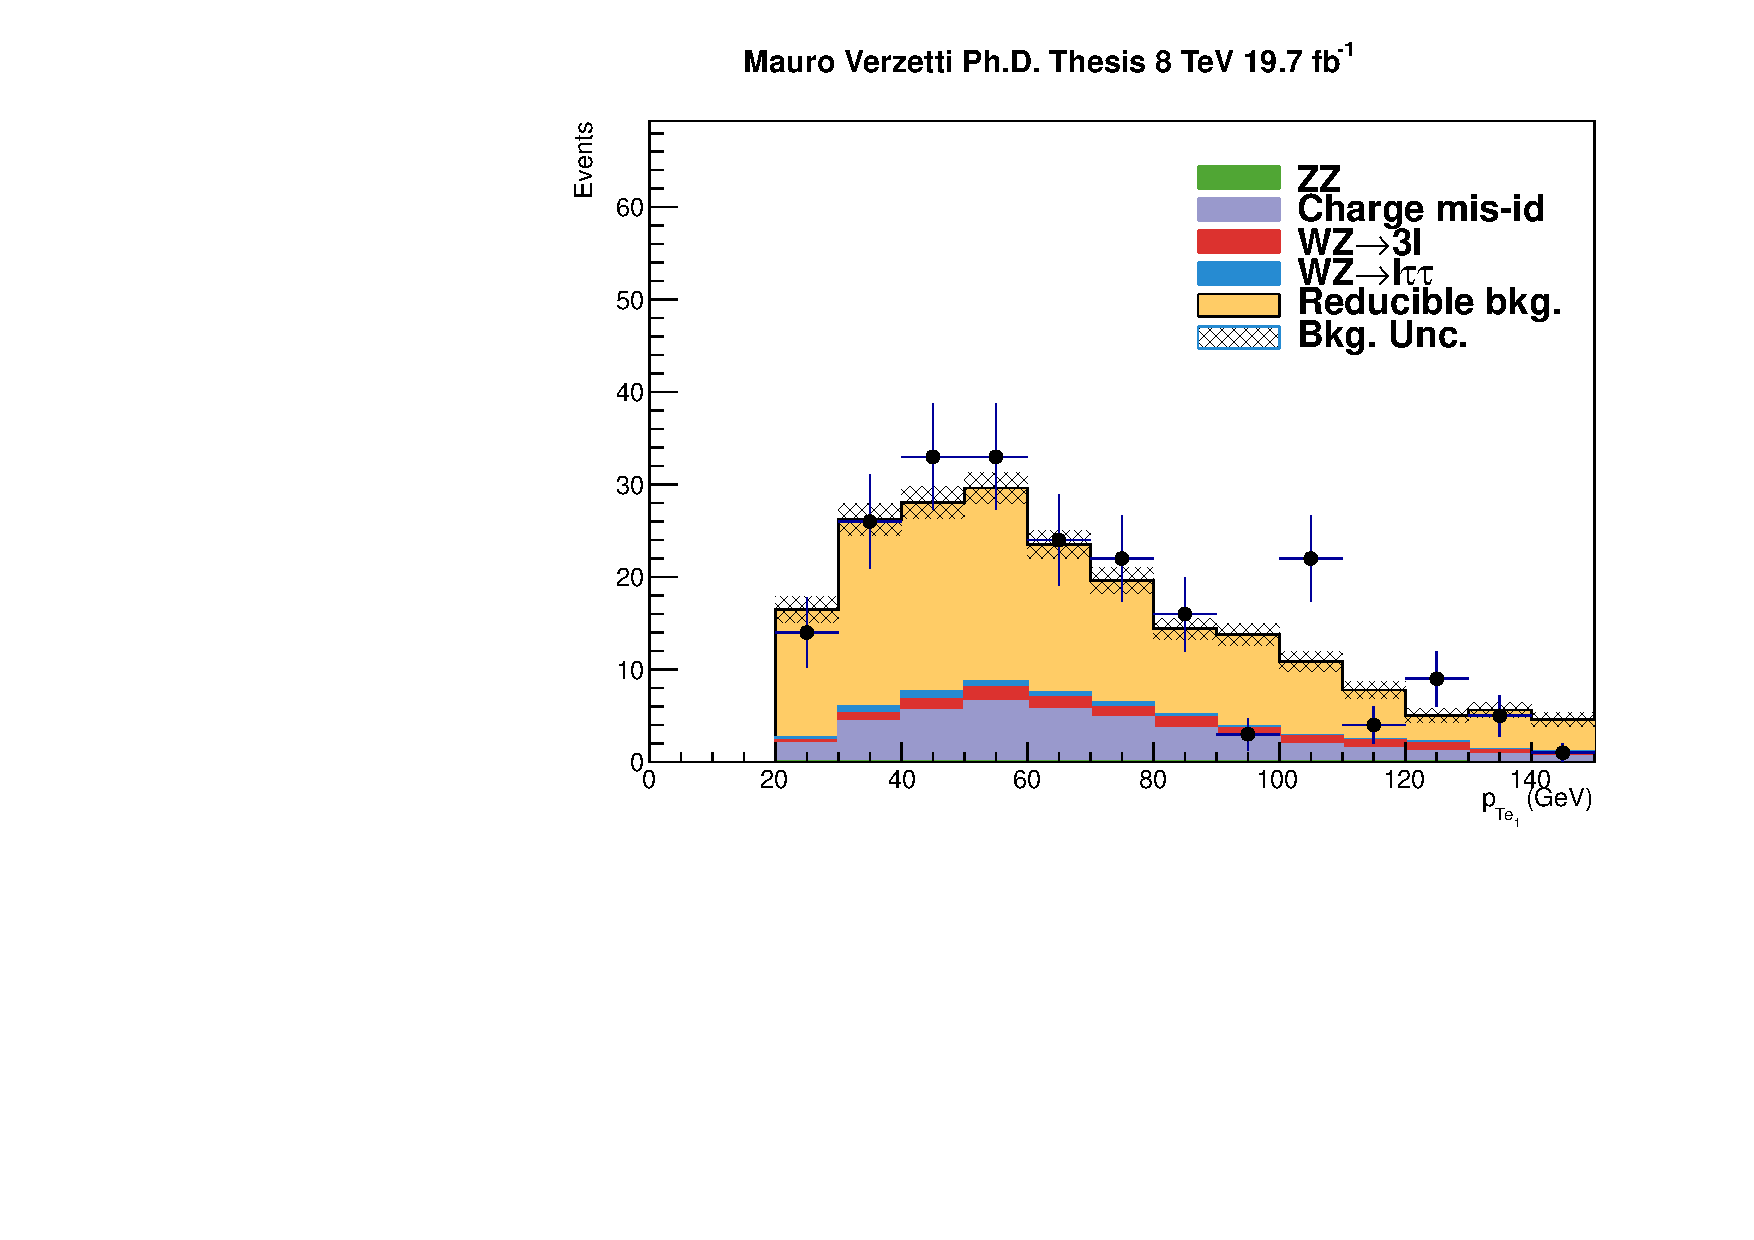
\includegraphics[width=0.49\textwidth]{4_Analisys/pics/8TeV/plots/eet/f3/Full/final-f3-e1Pt-Full.pdf}
  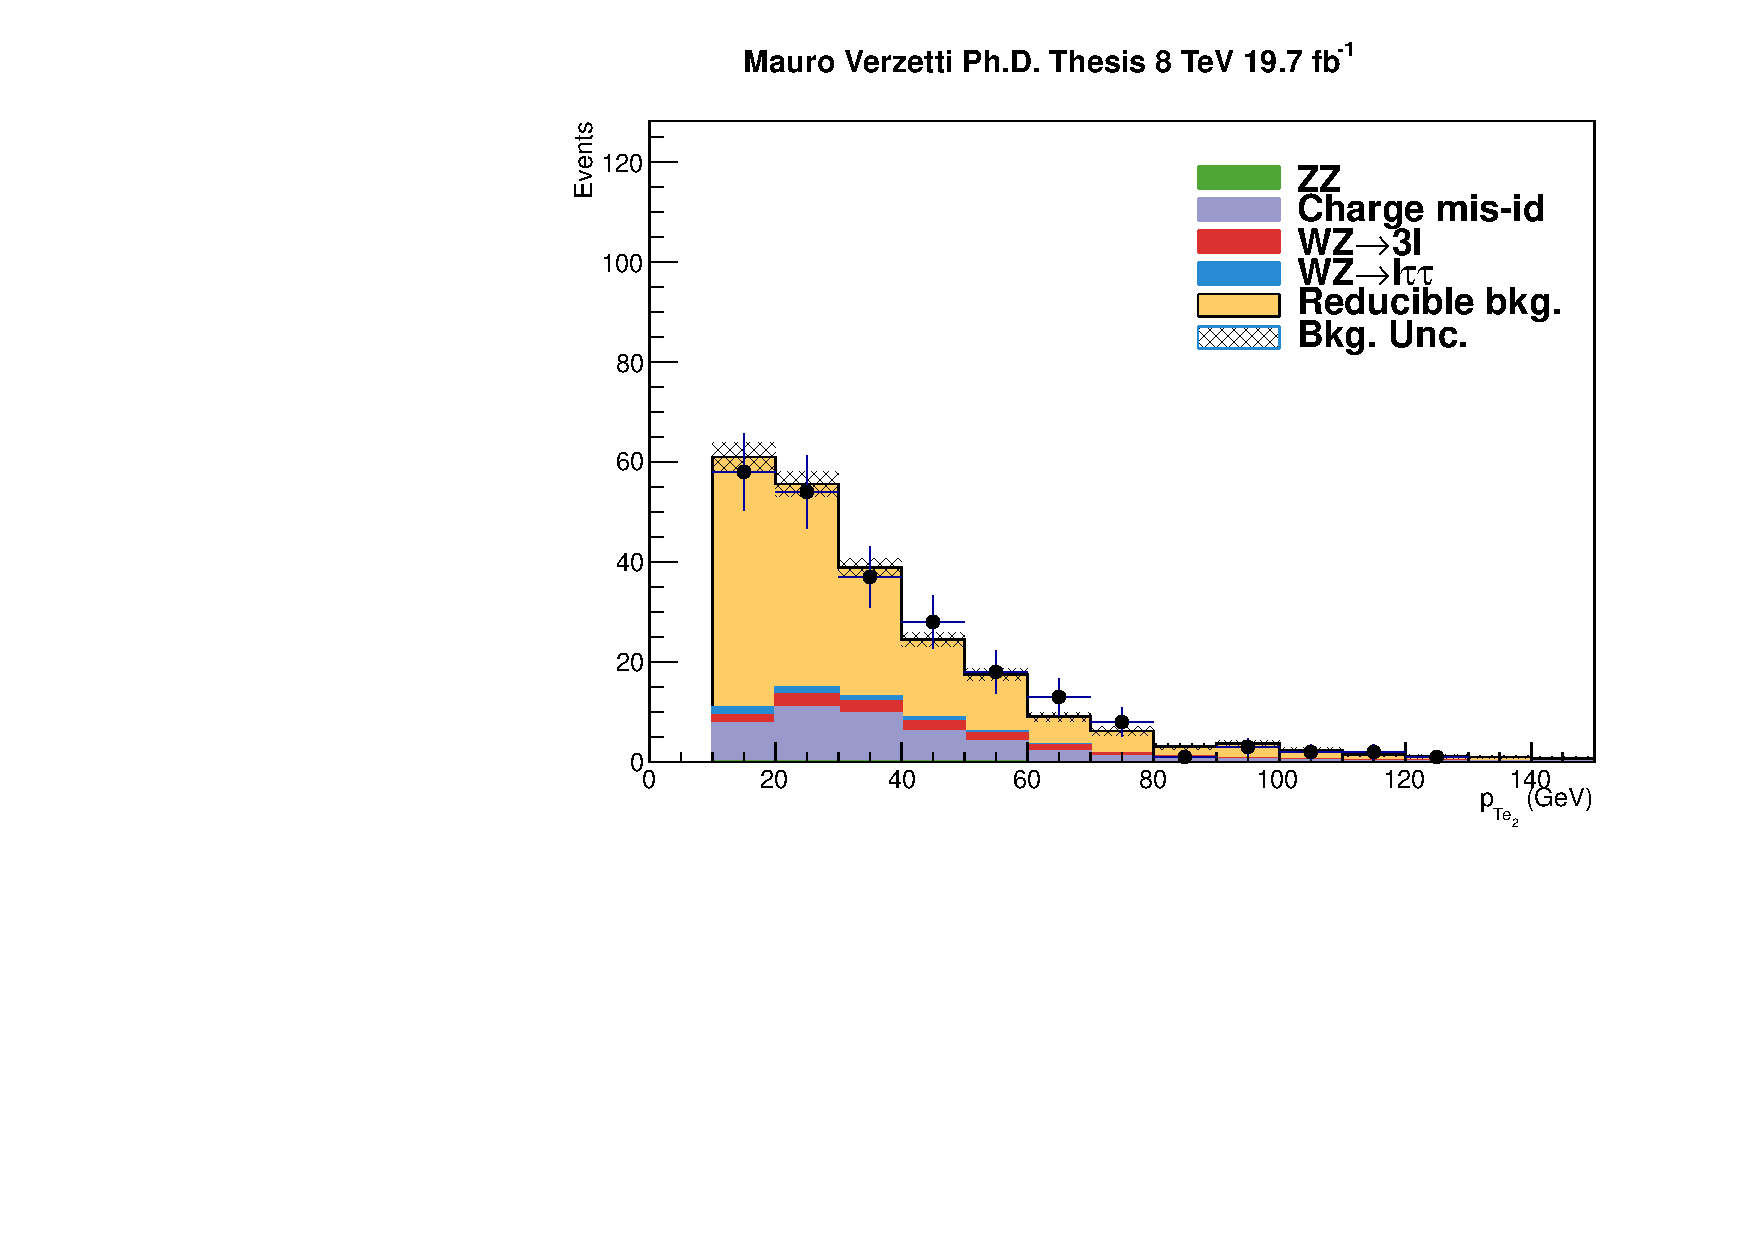
\includegraphics[width=0.49\textwidth]{4_Analisys/pics/8TeV/plots/eet/f3/Full/final-f3-e2Pt-Full.pdf}\\
  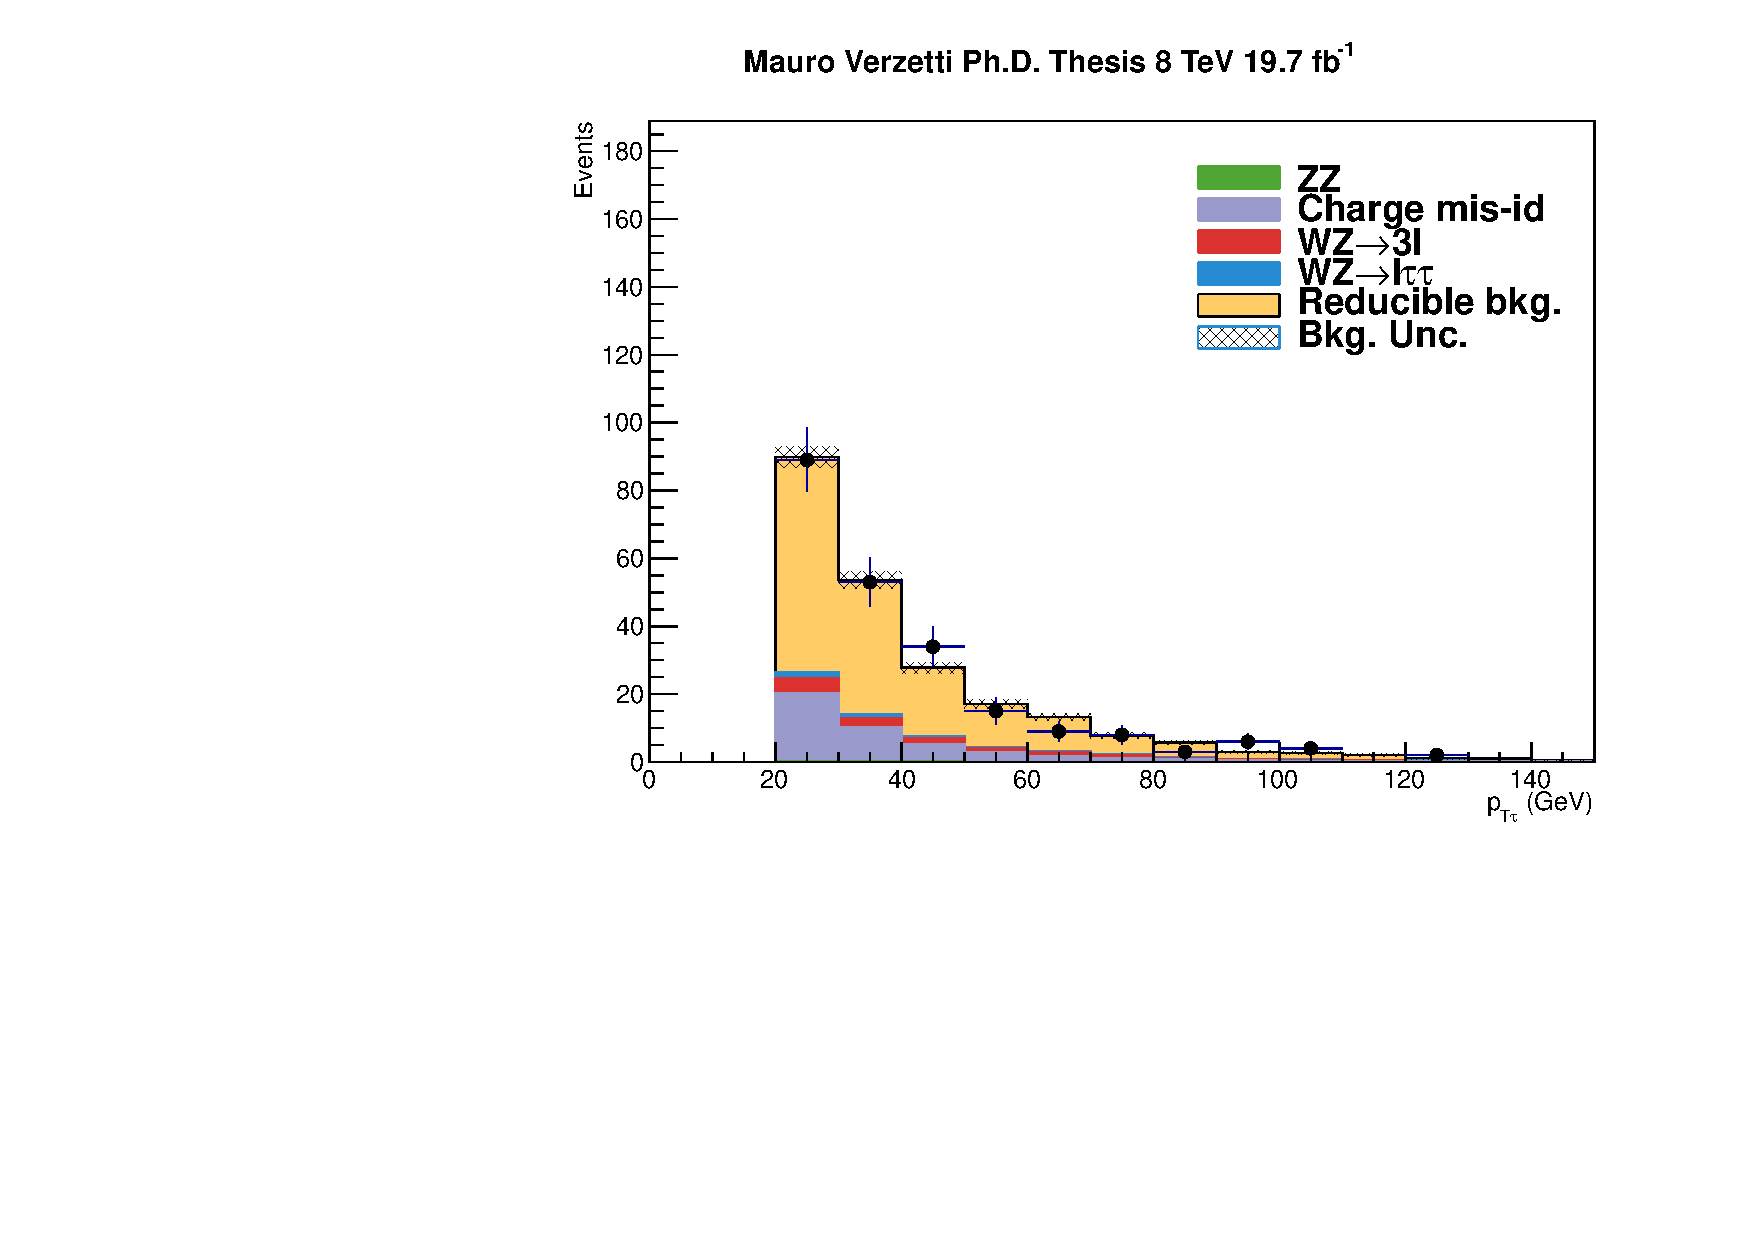
\includegraphics[width=0.49\textwidth]{4_Analisys/pics/8TeV/plots/eet/f3/Full/final-f3-tPt-Full.pdf}
  \caption{Comparison of measured and predicted backgrounds in the $ee\tau_h$ ``fake tau'' control region for 8 TeV data.
  From top left to bottom: mass of the sub-leading electron and the tau system, scalar sum of the leptons \pT ($L_T$), \pT of the leading and sub-leading electron, and \pT of the hadronic tau.
  The reducible background contribution is estimated by the kNN method, as in the signal region.
  The shaded band represents the uncertainty on the sum of the background contributions.
  }
  \label{fig:LLT_eet_f3_control_8TeV}
\end{center}
\end{figure}

\subsection{Fake tau method}

To better estimate the solidity of the the ``fake lepton'' method against differences in composition of the training sample and the sample to which the method is applied, a second background estimate is performed.
This methodology is very similar to the previous one, but the object considered as possibly mis-reconstructed is the hadronic tau.

\subsubsection{Region definition}

The misidentification probability for $\tau_h$ candidates is measured in $W+$Jets events, requiring:
\begin{itemize}
\item Events must pass the single muon trigger;
\item A muon candidate with $\pt > 24$ GeV and $|\eta| < 2.1$;
\item The muon must pass the tight Particle Flow identification and have a combined PF Relative Isolation $\Delta \beta $ corrected below $0.1$;
\item The longitudinal impact parameter of the muon track with respect to the primary vertex must be less than 0.2 cm;
\item $M_{T}(\mu, \met) > 40\GeV$;
\item Two same sign tau candidates are required, both with opposite charge to the muon;
\item Events are rejected if they contain another muon or electron with $\pt > 15$ GeV;
\item Events are rejected if they contain a jet with $\pt > 20$ GeV and $|\eta|< 2.4$ satisfying the loose CSV b-tagging working point.
\end{itemize}
The tau fake-rate is measured individually for the 2011 and 2012 run periods in three regions of pseudo-rapidity ($|\eta|<0.8$,
\mbox{$0.8<|\eta|<1.6$} and $1.6<|\eta|<2.3$) and as a function of the tau \pT. The misidentification probability is modeled by a Landau function. % with peak and width left free to float.%, and an additive constant.
The width and peak parameters are adjusted to best match the measured $\rm{jet}\To\tau_h$ fake-rates.

The fake rates measured in the %measured tau misidentification rates in both 
7 TeV and 8 TeV data are shown in figure~\ref{fig:LLT_tau_FR}. The $\rm{jet}\To\tau_h$ fake-rate %measured tau misidentification rate 
ranges from 6\% at low tau \pT in the end-cap region, to 1\% at high \pT ($ > 80$ GeV) in the central region.

\begin{figure}
  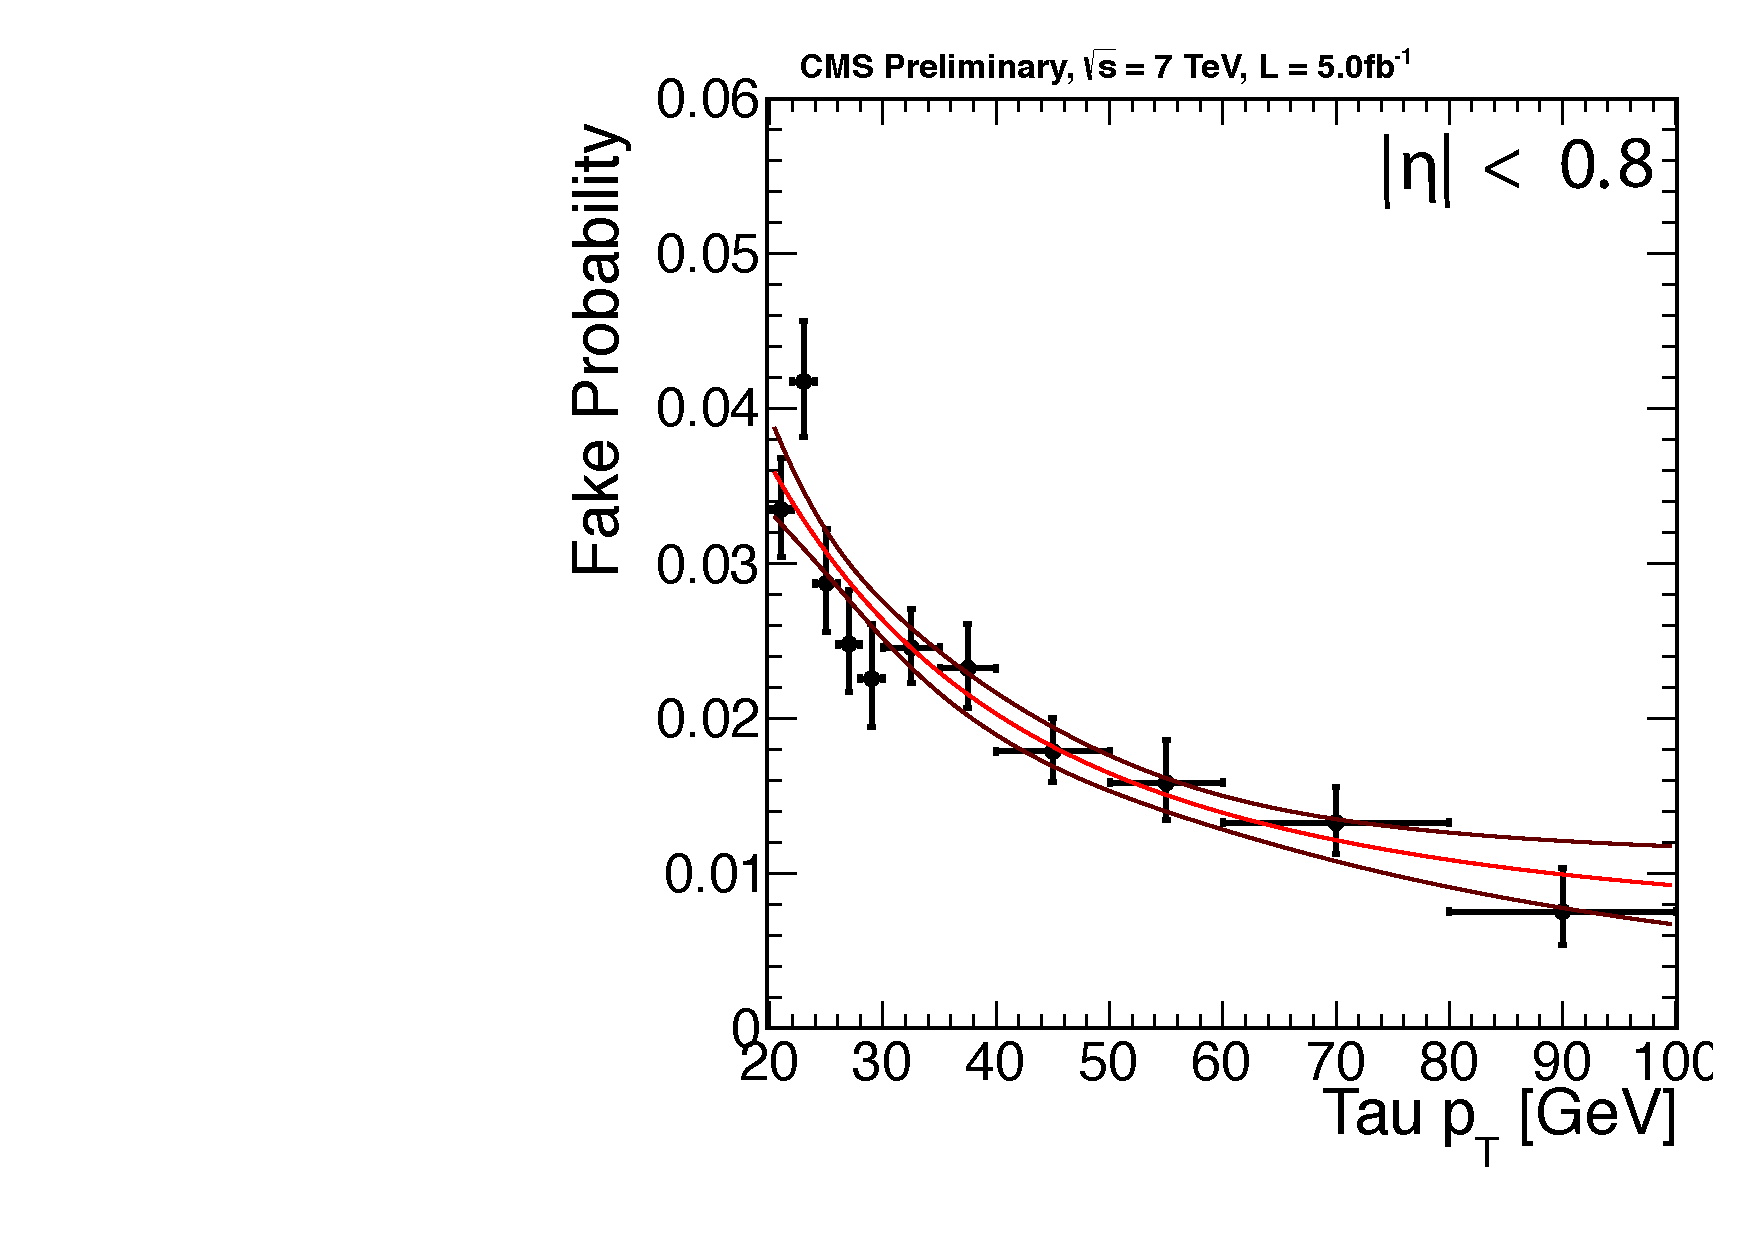
\includegraphics[width=0.33\textwidth]{4_Analisys/pics/7TeV/fakerate_fits/tau_fr_barrel.pdf}
  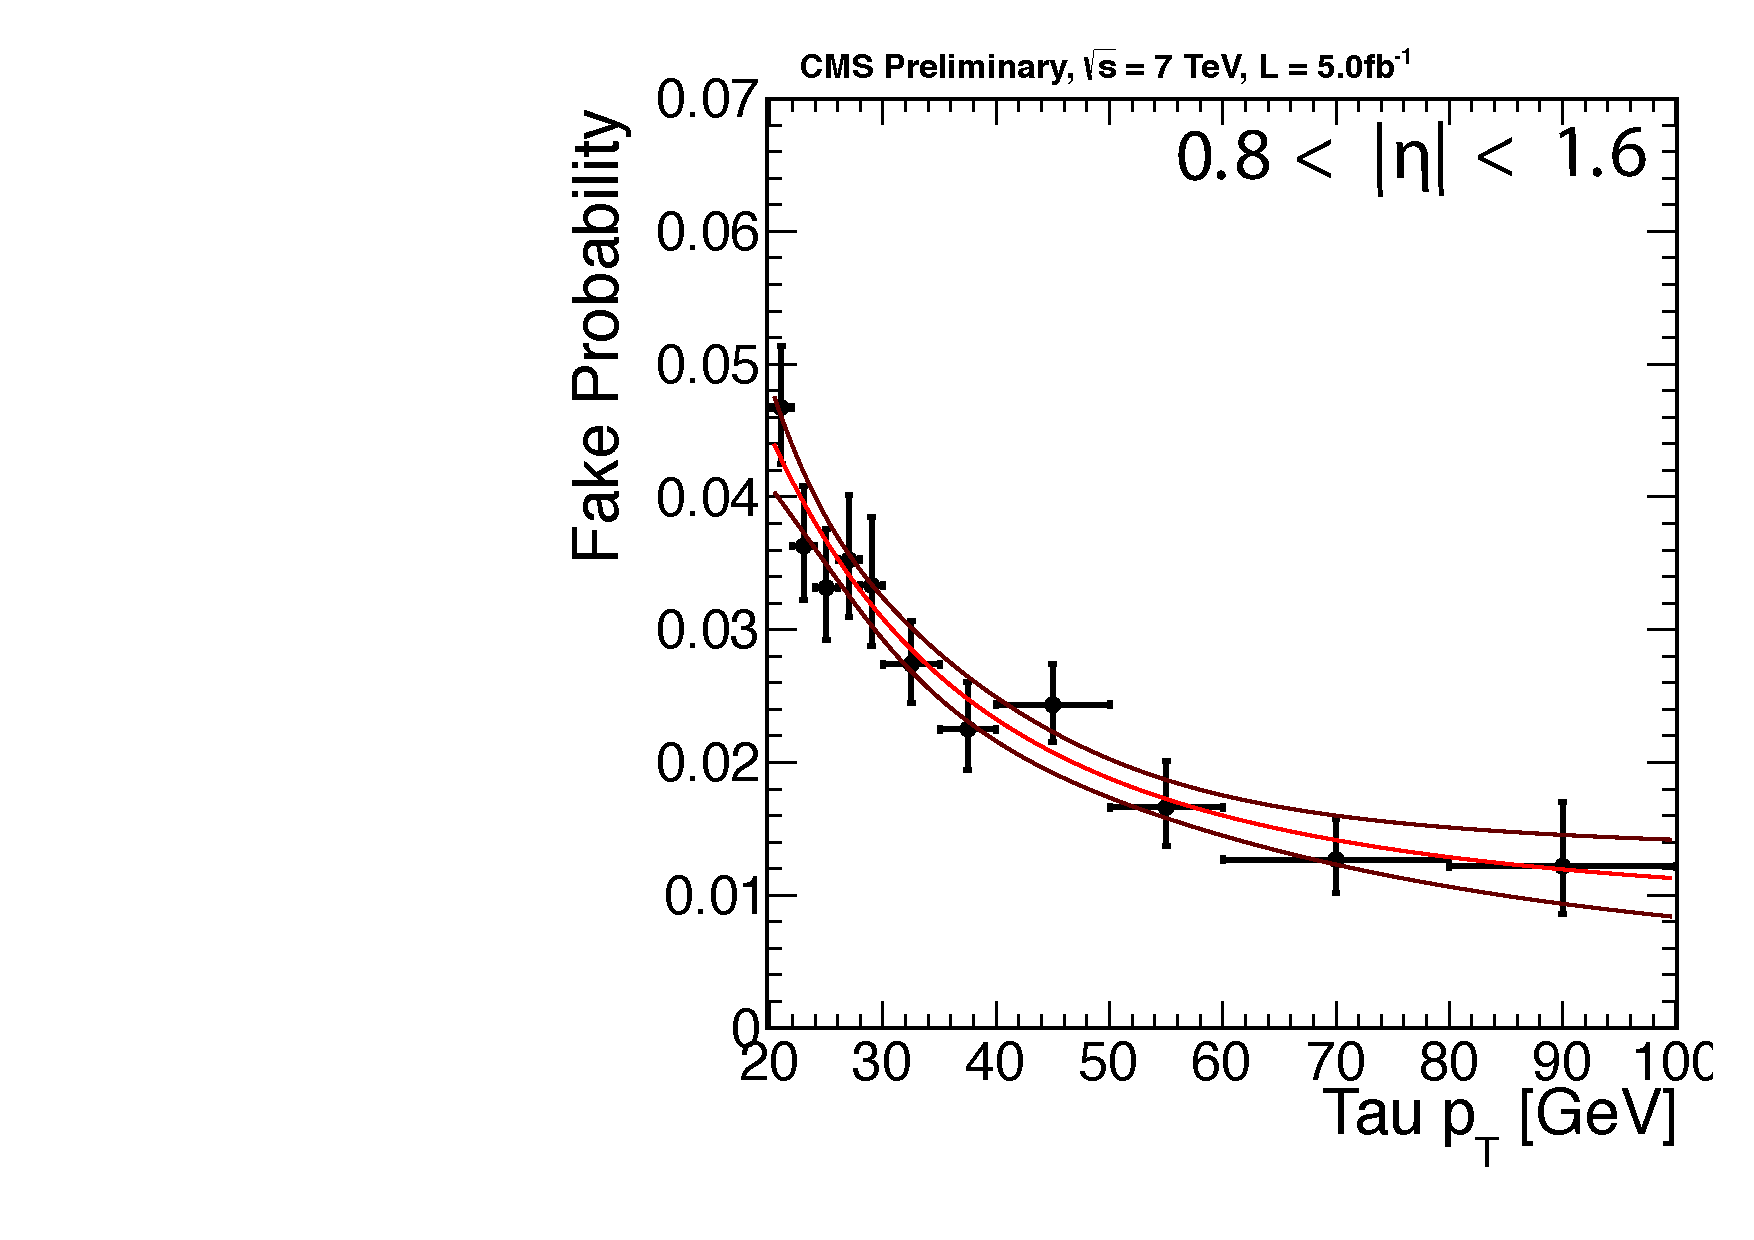
\includegraphics[width=0.33\textwidth]{4_Analisys/pics/7TeV/fakerate_fits/tau_fr_transition.pdf}
  \includegraphics[width=0.33\textwidth]{4_Analisys/pics/7TeV/fakerate_fits/tau_fr_endcap.pdf}\\
  \includegraphics[width=0.33\textwidth]{4_Analisys/pics/8TeV/fakerate_fits/tau_fr_barrel.pdf}
  \includegraphics[width=0.33\textwidth]{4_Analisys/pics/8TeV/fakerate_fits/tau_fr_transition.pdf}
  \includegraphics[width=0.33\textwidth]{4_Analisys/pics/8TeV/fakerate_fits/tau_fr_endcap.pdf}
  \caption{Jet $\to \tau_h$ misidentification probability in 7 TeV (top) and 8 TeV (bottom) data, in W$\to \mu$+jet events, as function of tau \pT in barrel (left), transition (center) and endcap (right) regions. The red line shows the result fit to the data.}
  \label{fig:LLT_tau_FR}
\end{figure}


\subsubsection{Background shape extraction}

The tau misidentification probability is used to determine a second and completely independent estimate of the reducible background in the signal region.
In this method the tau is considered the possibly misidentified object. Events passing all the analysis selection criteria plus the loose tau
selection but \emph{not} the tight one are weighted according to the measured tau misidentification probability to estimate the reducible background.

This method only takes into account those processes in which jets are misidentified as taus. The method cannot account for the Drell-Yan, WW and $t\anti{t}$ reducible backgrounds
in which the reconstructed $\tau_h$ corresponds to a genuine hadronic tau or to an isolated light lepton faking a tau. To account for these types of background the method described in Section~\ref{sec:fakemethod}
is applied to simulated events. This procedure is considered to be more reliable than taking the MC expectation in the signal region directly.

The fake tau method was found to produce results consistent with the fake-rate method applied to leptons. To account for possible residual differences,
the fake lepton method is used as nominal value for the reducible background and the estimate obtained from the fake-tau method is used as systematic uncertainty on the background shape.

\subsection{Electron charge mis-identification}
\label{sec:charge_misid}

The most common reason for the mis-measurement of the electron charge inside the CMS detector is the interaction of such particle with material in the tracking detectors. % of an  is incorrectly assigned mostly due to a radiative process. 
An electron can radiate a photon, carrying most of its momentum, which may subsequently convert into an $e^+e^-$ pair with highly unbalanced momenta, producing an electron with charge opposite to the initial one that carries most of the initial energy. %If these two processes happen 
In case the bremsstrahlung and the photon conversion processes occur 
in proximity to the interaction point, the reconstruction algorithm cannot identify the electron as originating from a conversion.
The description of this process in the simulation is handled by \textsc{GEANT}~\cite{geant}. The probability for an electron to be reconstructed with opposite charge is measured as a function of the electron $\eta$ and \pT using a $\Z \rightarrow ee$ MC sample. The results are shown in figure~\ref{fig:charge_flip_prob_map}.

Another effect associated to the charge mis-measurement is a partial energy loss by radiation that fails to get associated to the electron candidate by the reconstruction algorithm.
This effect causes a shift of the dielectron invariant mass spectrum.
The precision with which this phenomenon is modeled in the simulation is not totally satisfactory. To quantify the effect, the spectra of opposite sign (OS) and same sign (SS) electron pairs were fitted with a Cruijfian function (a two-sided gaussian with exponential tails) allowing only a global shifting factor to float. The results of these fits are shown in figure~\ref{fig:ee_invMass_fit}. The process is repeated for both data and simulated events. The value extracted from the former is taken as central value, while the one taken from the latter is used as systematic uncertainty.

The probability for the electron charge mis-measurement is applied as a weight on opposite sign $e^\pm e^\mp \tau_h$ events, which pass the same selection as the signal region, in order to obtain a data-driven estimate for this type of background. The invariant mass distribution obtained with this method is artificially shifted towards lower values 
by the amount computed in the $\Z \rightarrow ee$ data.

\subsection{Control regions}

The background induced by charge misassignment is validated in a dedicated $\Z \To e^\pm e^\pm$ control region.
This region has the same selection as the $ee\tau_h$ signal region with the exception that events containing a tau are removed.
The di-electron invariant mass spectrum in this region is shown in figure~\ref{fig:control_Zee}. The red histogram represents opposite-sign dielectron events weighted by the charge misassignment probability and with the invariant mass scaled by an offset extracted from MC simulation.

\begin{figure}
  \begin{center}
  \includegraphics[width=0.8\textwidth]{4_Analisys/pics/8TeV/fakerate_fits/charge_flip_prob_map_eid12Medium_h2taucuts.pdf}
  \caption{
  Electron charge misassignment probability (color scale) as a function of $|\eta|$ and \pT.}
  \label{fig:charge_flip_prob_map}
  \end{center}
\end{figure}


\begin{figure}
  \includegraphics[width=0.5\textwidth]{4_Analisys/pics/8TeV/fakerate_fits/charge_flip_prob_map_eid12Medium_h2taucutsos_trkMass.pdf}
  \includegraphics[width=0.5\textwidth]{4_Analisys/pics/8TeV//fakerate_fits/charge_flip_prob_map_eid12Medium_h2taucutsss_trkMass.pdf} \\
  \includegraphics[width=0.5\textwidth]{4_Analisys/pics/8TeV/fakerate_fits/charge_flip_prob_map_dataos_trkMass.pdf}
  \includegraphics[width=0.5\textwidth]{4_Analisys/pics/8TeV//fakerate_fits/charge_flip_prob_map_datass_trkMass.pdf} \\  
  \caption{
  Comparison of the fit to dielectron invariant mass distributions for opposite-sign (left) and same-sign (right) dielectron candidates from Drell--Yan MC simulation (top) and $\Z\To ee$ data (bottom). The measured invariant mass scale factor is 0.7\% for simulated events and 1.2\% for data}
  \label{fig:ee_invMass_fit}
\end{figure}

\begin{figure}
  \begin{center}
  \includegraphics[width=0.8\textwidth]{4_Analisys/pics/8TeV/plots/zee/EE_Charge_Flip_xcheck_trk_invMass.pdf}
  \caption{Invariant mass distribution of same-sign dielectron events: the red histogram is obtained using the information extracted from simulation
(charge misassignment probability and invariant mass scale correction) and applied them to opposite-sign data. The yellow histogram is obtained by applying the fake lepton method to estimate the reducible background.}
  \label{fig:control_Zee}
  \end{center}
\end{figure}

\section{Systematics uncertainties and category optimization}
\label{sec:systematics}

The optimization of the analysis sensitivity and the description of the systematic uncertainties are two subjects that are tightly bound. The figure of merit for %to maximize in 
the optimization is the expected signal significance, while considering the full set of uncertainties correlated with both signal and backgrounds. An optimization purely based on the ``statistical'' significance, defined as $S = N_{sig} / \sqrt{N_{sig} + N_{bkg}}$, may yield an optimal configuration for which the systematic uncertainties are very large.

In this section the definitions and values necessary to have a complete picture of the category optimization process are briefly introduced. The systematic uncertainties are described after the optimization process.
%Once this process will have been fully detailed a more complete description of the systematic uncertainties and their values will be presented. 
A detailed description of how systematic uncertainties are treated to obtain the final result is left for the sections describing the statistical interpretation of the data.

\subsection{Category optimization}

Given the strong dependence of the mis-identification rate on the \pT of the object considered, in particular the hadronic tau, it is quite straightforward to try to improve the signal purity by increasing the threshold on the objects $p_T$. A better but correlated solution is to use as discriminating observable the scalar sum of the \pT of the three final state leptons, called $L_T$.  

Two types of systematic uncertainties in the background templates are considered in this analysis: normalization uncertainties, which affect only the overall yield of a background, and shape uncertainties, which also affect distribution of the background between bins.

Normalization uncertainties are assigned to account for uncertainties in the luminosity measurement, in the correction factors for the trigger emulation, in the identification and isolation efficiencies and in the theoretical cross-sections for all the simulated processes. Normalization uncertainties are also assigned to account for the limited size of the MC samples and the very limited size of the loose-but-not-tight samples that are used to estimate the reducible backgrounds. The last two sources of background are strongly dependent on the category selection and have to be recomputed for each tested configuration.

The difference between the reducible background shape computed with the fake lepton method and the one evaluated with the fake tau method is accounted for by introducing a shape uncertainty that is allowed to vary both the shape and the normalization of the reducible background. 
The same procedure is applied to the reducible background shapes computed with the optimal number of neighbors and the two inferred boundaries. 
Single bin fluctuations in the reducible background shape due to the limited statistics in the anti-isolated regions are separately accounted for by a separate shape uncertainty for each bin (also called \emph{bin-by-bin uncertainties}). Bin-by-bin uncertainties are not allowed to change the total yield of the background process, as this effect is collectively handled by the appropriate normalization uncertainty. It is evident that also these shape uncertainties are dependent on the category selection.

During the optimization two options were tested: either apply a cut rejecting all the events below a certain \LT\ threshold, or divide the events in two categories (called \LT-high and \LT-low) that get fitted simultaneously, increasing the total sensitivity of the analysis. 
For each \LT \ threshold tested, the expected frequentist significance of both options has been computed for a SM Higgs boson of 125 GeV. The \LT\ scan was performed by varying the cut threshold between 60 and 170 GeV in 10 GeV steps. 

The categorization is expected to perform \emph{at least} as well as the equivalent cut option, since the \LT-high category alone has the same statistical power as the corresponding cut case. The categorization choice, however, requires a significant amount of data in both the event categories in order for the optimization to be stable. For this reason the categorization option has not been investigated in case of the 7 TeV data. In the 8 TeV $ee\tau_h$ channel the difference between the two options was found to be negligible and therefore the more simple cut was chosen. Figure~\ref{fig:LT_scan} show the results of the threshold scans for the three channels in the two run periods, while table~\ref{tab:LT_options} shows the \LT\ threshold values that maximize the significance for each channel, the reported selection is used to extract the final result.

\begin{figure}
  \includegraphics[width=0.5\textwidth]{4_Analisys/pics/7TeV/limits/mmt.pdf}
  \includegraphics[width=0.5\textwidth]{4_Analisys/pics/8TeV/limits/mmt.pdf} \\
  \includegraphics[width=0.5\textwidth]{4_Analisys/pics/7TeV/limits/emt.pdf}
  \includegraphics[width=0.5\textwidth]{4_Analisys/pics/8TeV/limits/emt.pdf} \\
  \includegraphics[width=0.5\textwidth]{4_Analisys/pics/7TeV/limits/eet.pdf}
  \includegraphics[width=0.5\textwidth]{4_Analisys/pics/8TeV/limits/eet.pdf} \\
  \caption{Expected significance versus \LT\ threshold value for the $\mu\mu\tau_h$ (top), the $e\mu\tau_h$ (center), and the $ee\tau_h$ (bottom) channels in 7 TeV (left) and 8 TeV (right) datasets for two optimization options. The LT threshold is represented by the black dots, the separation of LT event categories by the red boxes.}
  \label{fig:LT_scan}
\end{figure}

\begin{table}
\begin{center}
\caption{Threshold values and categorization approach used in signal extraction for each channel and dataset.}
\label{tab:LT_options}
\begin{tabular}{c c c c}
\hline
Run period & Channel & Best approach & Threshold (GeV) \\
\hline
\multirow{3}{*}{ 7 TeV } & $\mu\mu\tau_h$ & \LT\ Cut & 80 \\	
& $e\mu\tau_h$ & \LT\ Cut & 90 \\
& $ee\tau_h$    & \LT\ Cut & 90 \\
\hline
\multirow{3}{*}{ 8 TeV } & $\mu\mu\tau_h$ & \LT\ Category & 100 \\	
& $e\mu\tau_h$ & \LT\ Category & 110 \\
& $ee\tau_h$    & \LT\ Cut & 70 \\
\hline
\end{tabular}
\end{center}
\end{table}


\subsection{Systematic uncertainties}

As mentioned previously, the sources of systematic uncertainties accounted for in this work can be divided into two groups: the ones affecting only the total normalization of a process, yielding a normalization uncertainty, and the ones also affecting the distribution of the events, yielding a shape uncertainty.

A 2.2\% (2.6\%) uncertainty~\cite{lumi-uncertainty} in the total integrated luminosity is applied to the 7 TeV (8 TeV) simulated samples, respectively. This uncertainty is correlated throughout all the simulated processes, categories and channels belonging to the same running period.
The theoretical uncertainties on %accounted for 
the diboson cross-sections amount to 4\% due to parton distribution function (PDF) plus 4\% due to the QCD renormalization scale. These uncertainties are correlated between all the diboson processes, regardless of channel, category or running period.

The statistical power of the different simulated samples are accounted for by a normalization uncertainty that varies between 3 and 10\% and is uncorrelated between all the channels and categories.

The theoretical uncertainty on the signal cross section due to missing higher orders %the unknown QCD scale 
and due to parton distribution function amounts to 2.7\%~\cite{LHCHiggsCrossSectionWorkingGroup:2011ti}.

The uncertainties on the $e$ and $\mu$ identification, isolation, and trigger efficiencies correspond to the uncertainties on the data-to-simulation correction factors, which have been measured via the tag-and-probe technique\footnote{In a similar manner to what has been described in Section~\ref{sec:tauid_eff}, $\Z \To \ell \ell$ events are selected with a single lepton trigger and the desired isolation and identification working points are applied on both leptons. Additionally the invariant mass of the two leptons is required to be within the Z boson mass window: $60 < m_{\ell\ell} < 120$. The trigger efficiencies are computed by applying the trigger requirement to the probe lepton, which does not fire the trigger, both on data and MC. The discrepancies between the two efficiencies, binned in \pT and $\eta$ of the lepton, are applied as a scale factor on the MC and the uncertainty on such correction are taken as systematic uncertainties. A similar tag-and-probe approach on $\Z \To \ell \ell$ events is taken also to correct for discrepancies in the identification and isolation efficiencies.}.
The uncertainty on the $\tau$ identification efficiency is 6\% (see Section~\ref{sec:tauid_eff}).
The effect on the simulated yields due to the uncertainty on the electron and $\tau_h$ energy scale has been evaluated.
The electron energy scale uncertainty (1\% for $|\eta| < 1.5$, 2.5\% elsewhere) does not have a measurable effect on the analysis.
Varying the $\tau_h$ energy scale (within a 3\%~\cite{H_tautau} uncertainty) is found to change the expected yields by $3\%$, but has no sizable effect on the observables shapes. A 3\% normalization uncertainty is therefore included.
The uncertainty in the compatibility between simulated and measured efficiency of a light quark or gluon jet to be misidentified as a b-tagged jet, causing the b-veto to 
fail is propagated to the analysis and found to be covered by a 1\% uncertainty in the yields of the simulated samples.

Uncertainties in the reducible background estimation related to the choice of the number of neighbors, $k$, of the kNN algorithm and in the statistical power of the training sample are computed as described in section~\ref{sec:kNN_uncertainties} and propagated to the signal region as a shape uncertainty, which is also allowed to affect the total normalization of the process. The uncertainty is correlated between categories belonging to the same channel and running period.

Uncertainties due to the limited statistical power of the inverted isolation regions that are used to compute the reducible background shape are accounted for by introducing an additional normalization uncertainty that ranges between 12\% and 52\% plus bin-by-bin shape uncertainties. These uncertainties are uncorrelated between all categories and channels.

Finally, the possible mis-modeling caused by the differences in background processes composition between the kNN training sample and the isolation-inverted region is estimated with the ``fake tau'' method and applied as a shape uncertainty, uncorrelated between the different channels and categories.

A 4\% (7\%) uncertainty for each electron candidate in the final state is assigned to account for systematic uncertainties on the charge mis-measurement background yield in addition to the statistical power of the sample for 8 TeV and 7 TeV data, respectively. A 42\% (89\%) uncertainty is assigned to the invariant mass scaling factor (described in section~\ref{sec:charge_misid}) that is applied to the shape templates for the charge mis-measured background in the 8 TeV and 7 TeV data, respectively. The uncertainty is applied as a shape uncertainty with no normalization effect. %Both the uncertainties are uncorrelated between channels and running periods. 

A summary of the sources of systematic uncertainties, their values, and their treatment is given in table~\ref{tab:systematics}.

\begin{table}
  \begin{center}
    \caption{Systematic uncertainties affecting the $\ell\ell\tau_h$ categories. Values specific to the 2011 datasets are indicated in paranthesis.}
    \label{tab:systematics}
    \begin{tabular}{c c c c}
      \hline
      Source                  & Value & Type & Correlation\\
      \hline
      Luminosity              & $2.2\% (2.6\%)$ & norm. & correlated between channels \\
      $\sigma_{\rm WZ}$        & $4\% \oplus 4\%$  & norm. & fully correlated\\
      $\sigma_{\rm ZZ}$        & $3.3\% \oplus 2.3\%$   & norm. & fully correlated\\
      %$\sigma_{\rm ttW,WWW}  $                  & $100\%$\\
      $\sigma_{\rm H}$ (PDF)   & $2.7\%$  & norm. & fully correlated \\
      diboson MC statistics & $[3\% - 9\%]$ & norm. & fully uncorrelated \\
      signal MC statistics & $[4\% - 12\%]$ & norm. & fully uncorrelated \\
%      \multirow{2}{*}{diboson MC statistics} & $[5\% - 7\%]$ depending on & \multirow{2}{*}{norm.} & \multirow{2}{*}{fully uncorrelated}\\
%      & sample and category & & \\
%      \multirow{2}{*}{signal MC statistics} & $[5\% - 7\%]$ depending on & \multirow{2}{*}{norm.} & \multirow{2}{*}{fully uncorrelated}\\
%      & sample and category & & \\ 
      Tau energy scale        & $3\%$   & norm. & correlated between categories\\
      Tau ID                  & $6\%$ & norm. & correlated between categories\\
      Muon ID + Iso           & $2\%$ & norm. & fully correlated \\
      Electron ID + Iso       & $2\%$ & norm. & fully correlated  \\
      b-tag Fake Rate         & $1\%$ & norm. & fully correlated  \\
      Trigger efficiency  & $1\%$ & norm. & correlated between periods  \\
      fake background statistics & [12\% - 52\%] & norm. & fully uncorrelated \\
      charge mis-ID statistics & [3\% - 26\%] & norm. & fully uncorrelated \\
      kNN training & -- & shape & uncorrelated between channels \\
      fake background composition & -- & shape & fully uncorrelated \\
      charge flip mass scale & -- & shape & uncorrelated between channels \\
      single bin fluctuations & -- & shape & fully uncorrelated \\
      \hline
    \end{tabular}
  \end{center}
\end{table}

\section{Results}

The checks and optimizations have been performed on control regions completely orthogonal to the signal region, or simply based on the expected distributions of known backgrounds. This procedure, called ``blind analysis'', is aimed at reducing as much as possible any bias originating from the choices done by the analyst. 
Once the analysis is considered final, the distribution of observed events in the signal region of each channel are unveiled. 

The physics observable used to discriminate between the signal and the different sources of background is the invariant mass of the visible products of the hadronic tau decay and the sub-leading lepton, $\rm{M}_{\ell_2 \tau}$. The choice of the sub-leading lepton has been found to be about 70\% correlated to the true Higgs decay product, estimated using simulated data. Other observables to assign the correct light lepton as Higgs decay product such as the transverse mass of the lepton and the MET, the lepton isolation or the $\Delta\phi$ between the lepton and the \MET\ have been investigated, but were found to yield inferior correlation with the true Higgs decay products.

The presence of a considerable missing energy source such as the neutrino produced in the W decay does not allow the exploitation of more refined mass reconstruction algorithms such as SVFit.

A summary of the different observed distributions, compared to the respective expectations, is shown in figures~\ref{fig:LLT_mmt_prefit}, \ref{fig:LLT_emt_prefit}, \ref{fig:LLT_eet_prefit} for the different channels, categories and run periods. Tables~\ref{tab:prefit_yields_table_8TeV} and~\ref{tab:prefit_yields_table_7TeV} summarizes the expected and observed yields in each category and run period.

\begin{figure}
\begin{center}
  \includegraphics[width=0.49\textwidth]{4_Analisys/pics/7TeV/plots/mmt/LTCut/final-subMass-LTCut.pdf}\\
  \includegraphics[width=0.49\textwidth]{4_Analisys/pics/8TeV/plots/mmt/LTLow/final-subMass-LTLow.pdf}
  \includegraphics[width=0.49\textwidth]{4_Analisys/pics/8TeV/plots/mmt/LTHigh/final-subMass-LTHigh.pdf}\\
  \caption{
  Comparison of $M_{\mu_2\tau}$ spectra observed in data and the background expectation %Comparison of measured and predicted backgrounds 
  in the $\mu\mu\tau_h$ signal region for 7 TeV data (top) and 8 TeV data (bottom). The 8 TeV data is split according the optimal categorization (LT-low on the left and LT-high on the right).
  }
  \label{fig:LLT_mmt_prefit}
\end{center}
\end{figure}

\begin{figure}
\begin{center}
  \includegraphics[width=0.49\textwidth]{4_Analisys/pics/7TeV/plots/emt/LTCut/final-subMass-LTCut.pdf}\\
  \includegraphics[width=0.49\textwidth]{4_Analisys/pics/8TeV/plots/emt/LTLow/final-subMass-LTLow.pdf}
  \includegraphics[width=0.49\textwidth]{4_Analisys/pics/8TeV/plots/emt/LTHigh/final-subMass-LTHigh.pdf}\\
  \caption{
    Comparison of $M_{\ell_2\tau}$ spectra observed in data and the background expectation %Comparison of measured and predicted backgrounds 
  in the $e\mu\tau_h$ signal region for 7 TeV data (top) and 8 TeV data (bottom). The 8 TeV data is split according the optimal categorization (LT-low on the left and LT-high on the right).
  }
  \label{fig:LLT_emt_prefit}
\end{center}
\end{figure}

\begin{figure}
\begin{center}
  \includegraphics[width=0.49\textwidth]{4_Analisys/pics/7TeV/plots/eet/LTCut_7TeV/final-subMass-LTCut_7TeV.pdf}
  \includegraphics[width=0.49\textwidth]{4_Analisys/pics/8TeV/plots/eet/LTCut_8TeV/final-subMass-LTCut_8TeV.pdf}\\
  \caption{
  Comparison of $M_{e_2\tau}$ spectra observed in data and the background expectation %Comparison of measured and predicted backgrounds 
  in the $ee\tau_h$ signal region for 7 TeV data (left) and 8 TeV data (right).
  }
  \label{fig:LLT_eet_prefit}
\end{center}
\end{figure}


\begin{sidewaystable}
%\begin{table}
\caption{Expected event yields for the different background processes and for a 125 GeV WH, $\rm{H}\To\tau\tau$ signal compared to the number of events observed in the data, split by channel and category, for 8 TeV data. The uncertainty quoted in each background process represents statistical plus systematic uncertainty.
%considered in the analysis and number of observed events, divided by channel and category for 8 TeV data. The uncertainty quoted for each background process also includes normalization systematics
}
\begin{center}
\begin{tabular}{c c c c c c c c c}
\hline
\multirow{3}{*}{Process} & \multicolumn{5}{c}{Channels and event categories} \\
& \multicolumn{2}{c}{$\mu\mu\tau_h$} & \multicolumn{2}{c}{$e\mu\tau_h$} & \multirow{2}{*}{$ee\tau_h$} \\
& \LT Low & \LT High & \LT Low & \LT High & \\
\hline
WZ & $ 4.9 \pm 0.6 $ & $ 9.2 \pm 1.0 $ & $ 8.7 \pm 0.9 $ & $ 10.5 \pm 1.1 $ & $ 5.5 \pm 0.6 $ \\
ZZ & $ 0.44 \pm 0.04 $ & $ 0.57 \pm 0.06 $ & $ 0.71 \pm 0.07 $ & $ 0.72 \pm 0.07 $ & $ 0.43 \pm 0.04 $ \\
Reducible Bkg. & $ 9.0 \pm 1.4 $ & $ 6.5 \pm 1.2 $ & $ 9.4 \pm 1.4 $ & $ 8.1 \pm 1.3 $ & $ 7.8 \pm 0.9 $ \\
Charge mis-id. & -- & -- & $ 0.10 \pm 0.01 $ & $ 0.16 \pm 0.02 $ & $ 1.6 \pm 0.1 $ \\
WH, $\rm{H}\To\W\W$ & $ 0.047 \pm 0.004 $ & $ 0.109 \pm 0.009 $ & $ 0.073 \pm 0.006 $ & $ 0.16 \pm 0.01 $ & $ 0.072 \pm 0.006 $ \\
\hline
Total bkg. & $ 14.6 \pm 1.6 $ & $ 17.5 \pm 1.6 $ & $ 19.4 \pm 1.7 $ & $ 21.1 \pm 1.8 $ & $ 16.0 \pm 1.2 $ \\
\hline
WH, $\rm{H}\To\tau\tau$ ($m_\rm{H}=125$ GeV) & $ 0.25 \pm 0.04 $ & $ 1.2 \pm 0.1 $ & $ 0.56 \pm 0.06 $ & $ 1.4 \pm 0.1 $ & $ 0.62 \pm 0.07 $ \\
\hline
Observed & 14 & 12 & 24 & 17 & 13 \\
\hline
\end{tabular}
\end{center}

\label{tab:prefit_yields_table_8TeV}
\end{sidewaystable}
%\end{table}

%\begin{sidewaystable}
\begin{table}
\caption{%Expected yields for the different signal and background processes considered in the analysis and number of observed events, divided by channel and category for 7 TeV data. The uncertainty quoted for each background process also includes normalization systematics
Expected event yields for the different background processes and for a 125 GeV WH, $\rm{H}\To\tau\tau$ signal compared to the number of events observed in the data, split by channel and category, for 7 TeV data. The uncertainty quoted in each background process represents statistical plus systematic uncertainty.}
\begin{center}
\begin{tabular}{c c c c c c c c c}
\hline
\multirow{2}{*}{Process} & \multicolumn{3}{c}{Channels} \\
& $\mu\mu\tau_h$ & $e\mu\tau_h$ & $ee\tau_h$ \\
\hline
WZ & $ 2.3 \pm 0.3 $ & $ 3.6 \pm 0.4 $ & $ 1.2 \pm 0.1 $ \\
ZZ & $ 0.43 \pm 0.04 $ & $ 0.64 \pm 0.07 $ & $ 0.24 \pm 0.02 $ \\
Reducible Bkg. & $ 0.4 \pm 0.2 $ & $ 1.2 \pm 0.5 $ & $ 1.2 \pm 0.3 $ \\
Charge mis-id. & -- & $ 0.04 \pm 0.01 $ & $ 0.38 \pm 0.06 $ \\
WH, $\rm{H}\To\W\W$ & $ 0.035 \pm 0.003 $ & $ 0.055 \pm 0.005 $ & $ 0.020 \pm 0.002 $ \\
\hline
Total bkg. & $ 3.5 \pm 0.4 $ & $ 6.0 \pm 0.7 $ & $ 3.3 \pm 0.3 $ \\
\hline
WH, $\rm{H}\To\tau\tau$ ($m_\rm{H}=125$ GeV) & $ 0.33 \pm 0.03 $ & $ 0.45 \pm 0.05 $ & $ 0.18 \pm 0.02 $ \\
\hline
Observed & 3 & 4 & 5 \\
\hline
\end{tabular}
\end{center}

\label{tab:prefit_yields_table_7TeV}
%\end{sidewaystable}
\end{table}


\section{Limit setting procedure and results}

\subsection{Statistical framework}
The binned $\rm{M}_{\ell_2 \tau}$ distributions of each channel and category have been used for the statistical interpretation of the results. The choice of the binning, reflected in the plots shown in the previous section, represents a compromise between granularity and event population of each bin. The final choice for 8 TeV data is 10 GeV wide bins between 20 and 80 GeV followed by a 20 GeV wide bin up to 100 GeV and a 30 GeV wide bin up to 130 GeV; finally a 70 GeV wide bin covers the invariant mass region between $130 < M_{\ell 2 \tau} < 200$ GeV. In the 7 TeV data, the small dataset size forces a much wider binning, leading to the choice of a 20 GeV wide bin between 20 and 40 GeV, followed by 40 GeV wide bins up to 120 GeV plus a single bin extending up to 200 GeV.

The expected background and signal distributions are fitted to the data to infer the value of the signal normalization, $\mu$, by maximizing a likelihood function.
The likelihood function is formulated in terms of $\mu \cdot s(\boldtheta) + b(\boldtheta)$, where $b(\boldtheta)$ denotes the expected background yield and distribution, while $s(\boldtheta)$ denotes the expected distribution of the signal process. Both $b(\boldtheta)$ and $s(\boldtheta)$ depend on the ensemble of \emph{nuisance parameters} ($\boldtheta$), which represent the statistical and systematic uncertainties in the predictions. The multiplicative $\mu$ parameter in front of $s(\boldtheta)$, known as \emph{signal strength modifier}, is the parameter of interest which describe the strength of the observed signal with respect to the expected SM value ($\sigma_{obs}/\sigma_{SM}$). The value of the $\mu$ parameter is allowed to become negative to avoid any bias in the fit.

The likelihood implemented in the fit is defined as the product of the likelihoods for each category times the likelihood function for the nuisance parameters:

\begin{eqnarray}
\mathcal{L}(obs|\mu, \boldtheta) &=& \prod^{cat} \mathcal{L}_c(obs|\mu, \boldtheta) \times \prod^{nuisance} p(\hat{\theta},\theta) \nonumber \\
&=& \prod^{cat} \operatorname{Poisson}(obs_c, \mu, \boldtheta) \times \prod^{nuisance} p(\hat{\theta},\theta),
\end{eqnarray}

%\begin{equation}
%\mathcal{L}(obs|\mu, \boldtheta) = \prod^{cat} \mathcal{L}_c(obs|\mu, \boldtheta) \times \prod^{nuisance} p(\hat{\theta},\theta) = \operatorname{Poisson}(obs_c, \mu, \boldtheta) \times %\prod^{nuisance} p(\hat{\theta},\theta),
%\end{equation}

where

\begin{equation}
\operatorname{Poisson}(obs_c, \mu, \boldtheta) = \dfrac{(\mu s_i(\boldtheta) + b_i(\boldtheta))^{n_i}}{n_i!}e^{(\mu s_i(\boldtheta) + b_i(\boldtheta))}.
\end{equation}

As described in section~\ref{sec:systematics}, two kinds of systematic uncertainties were considered. Systematic uncertainties associated to the overall normalization are considered to be distributed according to a \emph{log-normal} distribution:

\begin{equation}
\rho(\theta, \hat{\theta}) = \dfrac{1}{\theta\sqrt{2\pi}\opname{ln}(k)} e^{-\left(\dfrac{\opname{ln}(\theta/\hat{\theta})}{\sqrt{2}\opname{ln}k}\right)^2}
\end{equation}

with $k = 1+ \epsilon$, where $\epsilon$ is the size of the yield uncertainty.

Shape uncertainties are modeled using three distributions: the distribution for the central value plus the templates for the upward and downward shifts by one standard deviation of the respective nuisance parameter. A family of distributions is obtained starting from these three templates using a morphing technique. The morphing function interpolates the contents of each bin as a function of the nuisance parameter. The interpolation is quadratic within the boundaries provided by the two additional shifted templates and linear beyond this point. A gaussian distribution with mean 0 and $\sigma = 1$ is assigned to the single morphing parameter. The extrapolation is built in such a way that the nuisance parameter assumes the value 0 for the central template and the values $\pm1$ for the shifted templates. More details on this ``vertical morphing'' technique can be found in~\cite{Conway:2011in}.

In case the fit shows no significant presence of signal, which is related to a negative value of $\mu$ or compatible with zero, exclusion limits can be set.

The exclusion limit of a SM Higgs boson is statistically performed by evaluating the compatibility of the data to two hypotheses: the \emph{null hypothesis} $H_0$, which corresponds to the absence of a Higgs boson signal, and the  \emph{alternative hypothesis}, which includes the presence of a Higgs signal. The discrimination between the two hypotheses is performed by defining a test statistic under the null hypothesis and compute its value under the observed data case. The observed value of this test statistic, with respect to the theoretically expected distribution, allows to compute the probability to observe a compatibility to $H_0$ worse than the observed one. Such probability is called \emph{p-value} and is used to take the decision whether to reject the hypothesis $H_0$ in favor of $H_1$ or not.

The theoretical framework under which the test statistics is built represents a modified version of the CL$_s$ method~\cite{CLs} and follows the prescriptions agreed between the ATLAS and CMS statistical committees for Higgs boson searches~\cite{higgscombo}.

The null hypothesis is formulated in terms of only the expected backgrounds distributions $b(\boldtheta)$ defined previously, while 
the $H_1$ hypothesis is formulated as the sum of signal and backgrounds, $\mu \cdot s(\boldtheta) + b(\boldtheta)$, as initially shown.
%The setting of a 95\% confidence limit on the presence of the Higgs boson can therefore be reduced to the computation of the value $\mu_{up}$ which leads to $p(H(\mu_{up}\cdot s + b)) < 0.05$ with observed data.

According to the Neyman-Pearson lemma, the most powerful test statistics to discriminate between the $H_0$ (background only) and the $H_1$ (signal plus background) hypotheses is the \emph{profile likelihood ratio} $\lambda$, defined as:

\begin{equation}
\label{eq:likeratio}
\lambda(\mu) = -2 \operatorname{ln} \dfrac{\mathcal{L}(obs | \mu \cdot s + b, \thetahat_\mu)}{\mathcal{L}(obs | \muhat \cdot s + b, \thetahat)},
\end{equation}

%where $\thetahat$ and $\hat{\mu}$ are the set of nuisance values and the value of $\mu$ that maximize the likelihood (called \emph{maximum likelihood estimator}) and $\thetahat_\mu$ is the maximum likelihood estimator of the nuisances for a fixed value of $\mu$.
where $\thetahat$ represents the set of nuisance parameter values that maximize the likelihood (called \emph{maximum likelihood estimator}) and $\thetahat_\mu$ are the values of the nuisance parameters that maximize the likelihood for a fixed value of $\mu$.

Equation~\ref{eq:likeratio} is complemented by the boundary condition $0 \leq \muhat \leq \mu$ that ensures that the expected signal yield is positive and that the computed confidence interval is one sided (and therefore $\mu \geq \muhat$). These conditions are imposed on the test statistic by forcing $\muhat = 0$ even when the fit yields as best result a negative value and by setting the test statistic to 0 when $\mu < \muhat$.

\begin{equation}
q(\mu) = \left\{\begin{matrix}
-2 \operatorname{ln} \dfrac{\mathcal{L}(obs | \mu \cdot s + b, \thetahat_\mu)}{\mathcal{L}(obs | \muhat \cdot s + b, \thetahat)} & , \muhat < 0\\ 
-2 \operatorname{ln} \dfrac{\mathcal{L}(obs | \mu \cdot s + b, \thetahat_\mu)}{\mathcal{L}(obs | \muhat \cdot s + b, \thetahat)} & ,0 \leq \muhat \leq \mu \\ 
0 & , \mu < \muhat
\end{matrix}\right.
\label{eq:test_stat}
\end{equation}

%Under this definition small values of 
The test statistic $q(\mu)$ is defined such that small (large) values indicate preference for the $H_1$ ($H_0$) hypothesis.

%Under the assumption of large samples 
In the limit of large event statistics the distribution of the test statistic $q_\mu$ under both hypotheses collapse into well-defined analytical functions as described by the Wilkins theorem and reported in~\cite{Cowan:2010js, higgscombo}. This assumption allows to compute the p-value %, i.e. the probability to observe data less compatible with the null hypothesis than the observed one, 
under a specific hypothesis with a numerical integration rather than toy MC methods.

A naive approach to limit setting would be computing, for each mass point, the value $\mu_{up}$ for which $p(q(\mu_{up}) | H_1) = \int_{q_{\mu,obs}}^{\infty}f(q_\mu|H_{\mu_{up}})dq_\mu = 0.05$. This approach would not be safe in case of background under-fluctuations and a small expected signal. In this case the value $p(q(\mu_{up}) | H_0)$ is also a small number, potentially very close to the threshold of 0.05. This would lead to a paradox in which both $H_1$ \emph{and} $H_0$ have to be rejected.

In this situation data are not sufficient to reject the $H_1$ hypothesis. To overcome this effect the \CLs\ method defines the confidence level as:

\begin{equation}
CL_s(\mu) = \dfrac{CL_{s+b}}{CL_b} = \dfrac{p(q(\mu) | H_1)}{p(q(\mu) | H_0)}
\end{equation}

The immediate consequence of this definition is that small values of $\mu$ become harder to exclude.

\subsection{Fit results}

The reliability of the background modeling and of the systematic uncertainty model can be tested by analyzing the ancillary output of the profile maximum likelihood fit performed during the CL$_s$ limit computation. A common practice is to compute the values:

\begin{equation}
\dfrac{\hat{\theta} - \theta}{\sigma_{\theta}},
\end{equation}

which are the difference between the best-fit (post-fit) value and the central (pre-fit) value of the nuisance parameter, divided by its expected uncertainty. This quantity is commonly referred to as \emph{pull}. The maximum likelihood fit also evaluates the a posteriori variance of each nuisance parameter. Large outliers in the pull distribution can indicate an under-estimation of the systematic uncertainty associated to the corresponding nuisance parameter. Very small a posteriori variance of a nuisance indicates that the data are constraining a certain systematic uncertainty to a better degree than the a priori knowledge. This effect is not necessarily a flaw in the modeling, but requires additional scrutiny to ensure that the correlation of such nuisance parameter among different categories is well motivated. This effect is widely exploited when creating a category with large number of selected events and low sensitivity on the sole purpose of constraining one or more systematic effects on a more sensitive, but small size, category. 

Table~\ref{tab:pulls} summarizes the largest pulls observed in the maximum likelihood (ML) fit to the data.

\begin{table}
\caption{List of all the nuisance parameters which pull ($\Delta x/\sigma_{\text{in}}$) is either larger than $\pm0.3$ or the a posteriori variance ($\sigma_{\text{out}}/\sigma_{\text{in}}$) changed by more than 10\% with respect to the a priori one. $\Delta x$ denotes the shift in the nuisance value that best fits the data and $\sigma_{\text{in}}, \,\sigma_{\text{out}}$ represent the a priori and a posteriori variance of the nuisance parameter, respectively.}
\begin{tabular}{c c c c } \hline 
\multirow{2}{*}{ Sample } & \multirow{2}{*}{Channel} & \multirow{2}{*}{name} &     $b$-only fit \\
 &  & &  $\Delta x/\sigma_{\text{in}}$, $\sigma_{\text{out}}/\sigma_{\text{in}}$ \\  
\hline
\multirow{5}{*}{ 7 TeV } & \multirow{3}{*}{ $\mu\mu\tau_h$ } & Reducible bkg. Bin-by-bin bin \#2   &      -0.20, 1.08 \\
& & Reducible bkg. Bin-by-bin bin \#4      &      +0.14, 1.68 \\
& & kNN shape uncertainty           &      -0.04, 0.83 \\
 \cline{2-4}
& $e\mu\tau_h$ & Reducible bkg. Bin-by-bin bin \#1      &      +0.20, 0.85 \\
 \cline{2-4}
& $ee\tau_h$ & Reducible bkg. Bin-by-bin bin \#3      &      -0.31, 1.03 \\
 \hline
\multirow{11}{*}{ 8 TeV } & \multirow{3}{*}{ $\mu\mu\tau_h$ } & Reducible bkg. normalization, $L_T$ high   &      -0.30, 0.95 \\
& & Reducible bkg. composition, $L_T$ high    &      -0.35, 0.67  \\
& & Reducible bkg. Bin-by-bin bin \#1 &      +0.25, 0.88 \\
& & Reducible bkg. Bin-by-bin bin \#7 &      -0.35, 1.00 \\
& & Reducible bkg. composition, $L_T$ low     &      +0.32, 0.64  \\
& & kNN shape uncertainty          &      +0.25, 0.82  \\
 \cline{2-4}
& \multirow{4}{*}{ $\mu\mu\tau_h$ } & Reducible bkg. composition, $L_T$ high    &      +0.52, 0.74 \\
& & Reducible bkg. Bin-by-bin bin \#1 &      +0.32, 0.91 \\
& & Reducible bkg. composition, $L_T$ low     &      -0.45, 0.62  \\
& & kNN shape uncertainty          &      -0.03, 0.73  \\
 \cline{2-4}
& $ee\tau_h$ & Reducible bkg. composition           &      -0.52, 0.82 \\
 \hline
\end{tabular}

\label{tab:pulls}
\end{table}

The agreement between the data and the background description is also tested by the goodness of fit. It is computed by randomly sampling a set of pseudo-data, called \emph{toys}, from the expected distributions of the backgrounds, allowing for fluctuations within the variance of the nuisance parameters. These pseudo-data are then fit with the same background model to obtain a (toy) ``observed'' limit. 

The distribution of the limits computed with the toys is then compared with the one observed in the real data. The goodness of fit, as in the case of the $\chi^2$ method, is the right-sided integral of the distribution of toys, starting from the observed value. Figure~\ref{fig:gof} shows the goodness of fits for the different channels.

\begin{figure}
\begin{center}
  \includegraphics[width=0.49\textwidth]{4_Analisys/pics/GoF/mmt-goodness-of-fit-125.pdf}
  \includegraphics[width=0.49\textwidth]{4_Analisys/pics/GoF/emt-goodness-of-fit-125.pdf}\\
  \includegraphics[width=0.49\textwidth]{4_Analisys/pics/GoF/eet-goodness-of-fit-125.pdf}
  \includegraphics[width=0.49\textwidth]{4_Analisys/pics/GoF/vhtt_wh-goodness-of-fit-125.pdf}\\
  \caption{Goodness of fit as computed by toys for $\mu\mu\tau_h$ (top left), $e\mu\tau_h$ (top right), $ee\tau_h$ (bottom left), and combined (bottom right) fits. The blue arrow represents the value observed in data.}
  \label{fig:gof}
\end{center}
\end{figure}


Figures~\ref{fig:LLT_mmt_postfit}, \ref{fig:LLT_emt_postfit}, \ref{fig:LLT_eet_postfit} show the data and background distributions after the fitting process.

\begin{figure}
\begin{center}
  \includegraphics[width=0.49\textwidth]{4_Analisys/pics/postfit/mmt_postfit_7TeV_FitAllChannels.pdf}\\
  \includegraphics[width=0.49\textwidth]{4_Analisys/pics/postfit/mmt_low_postfit_8TeV_FitAllChannels.pdf}
  \includegraphics[width=0.49\textwidth]{4_Analisys/pics/postfit/mmt_high_postfit_8TeV_FitAllChannels.pdf}\\
  \caption{Comparison of measured and predicted $\rm{M}_{\ell_2\tau}$ distributions in the $\mu\mu\tau_h$ signal region for 7 TeV data (top) and 8 TeV data (bottom). 
  Expected backgrounds are shown for the post-fit values of the nuisance parameters. 
  The 8 TeV data are split according the optimal categorization.}
  \label{fig:LLT_mmt_postfit}
\end{center}
\end{figure}

\begin{figure}
\begin{center}
  \includegraphics[width=0.49\textwidth]{4_Analisys/pics/postfit/emt_postfit_7TeV_FitAllChannels.pdf}\\
  \includegraphics[width=0.49\textwidth]{4_Analisys/pics/postfit/emt_low_postfit_8TeV_FitAllChannels.pdf}
  \includegraphics[width=0.49\textwidth]{4_Analisys/pics/postfit/emt_high_postfit_8TeV_FitAllChannels.pdf}\\
  \caption{Comparison of measured and predicted $\rm{M}_{\ell_2\tau}$ distributions in the $e\mu\tau_h$ signal region for 7 TeV data (top) and 8 TeV data (bottom). 
  Expected backgrounds are shown for the post-fit values of the nuisance parameters. 
  The 8 TeV data are split according the optimal categorization.}
  \label{fig:LLT_emt_postfit}
\end{center}

\end{figure}
\begin{figure}
\begin{center}
  \includegraphics[width=0.49\textwidth]{4_Analisys/pics/postfit/eet_postfit_7TeV_FitAllChannels.pdf}
  \includegraphics[width=0.49\textwidth]{4_Analisys/pics/postfit/eet_postfit_8TeV_FitAllChannels.pdf}\\
  \caption{Comparison of measured and predicted $\rm{M}_{\ell_2\tau}$ distributions in the $e\tau_h$ signal region for 7 TeV data (top) and 8 TeV data (bottom). 
    Expected backgrounds are shown for the post-fit values of the nuisance parameters. }
  \label{fig:LLT_eet_postfit}
\end{center}
\end{figure}

The resulting shapes after the fitting process can be combined together to have a more complete view of the results. The combination is performed in such a way that each category contributes to the total by an amount that is proportional to its signal purity evaluated as $S / (S+B)$, where $S$ denotes the integral of the signal and $B$ the sum of the backgrounds as from pre-fit values. The total normalization of the shapes is kept constant: i.e. the integral of the observed data is not affected by this procedure. Given the differences in the choice of binning this combination is only possible among 7 TeV and 8 TeV categories separately. 

From this process, result of which is shown in figure~\ref{fig:sbweight}, one can see that the number of events observed in the mass region in which the Higgs signal is expected to appear is below the background expectation. %an under-fluctuation of the backgrounds is clearly visible.
Even though these plots have relatively limited statistical meaning, they help showcase the background under-fluctuation observed in the data.

\begin{figure}
\begin{center}
  \includegraphics[width=0.49\textwidth]{4_Analisys/pics/postfit/postfit_ssb_weight_7TeV.pdf}
  \includegraphics[width=0.49\textwidth]{4_Analisys/pics/postfit/postfit_ssb_weight_8TeV.pdf}\\
  \caption{$S / (S+B)$ weighted combination of post-fit results from 7 TeV (left) and 8 TeV (right) categories. The over-all normalization of data is kept constant.}
  \label{fig:sbweight}
\end{center}
\end{figure}

The computation of the $\mu$ values for the different channels and their combination confirms the background under-fluctuation. Figure~\ref{fig:mu_vals} shows the observed $\mu$ values for the three $\ell\ell\tau_h$ channels and their combination. Even though these values are negative, the combination is still compatible with the SM value $\mu = 1$. The right plot on figure~\ref{fig:mu_vals} shows the best fit $\mu$ values for each different $\rm{H}\To\tau\tau$ channel search performed by CMS.% The fluctuation observed in the $\ell\ell\tau_h$ channels described in this thesis is  into the spread observed among the larger amount of channels searched by CMS. 

As described in section~\ref{sec:higgs_res} the combination of these channels, including the ones presented in this thesis, led to the first observation of the SM Higgs boson into tau lepton pairs in CMS.

\begin{figure}
        \centering
	\includegraphics[width=0.49\textwidth]{4_Analisys/pics/limits/mu_values.pdf}
	\includegraphics[width=0.49\textwidth]{1_Introduction_Th_and_Exp/pics/BestFit_sm_per_chn.pdf}
       \caption{Best fit signal strength $\mu$ for the channels presented in this thesis (left) and those included in the CMS $\rm{H} \To \tau \tau$ search (right) and their respective combined value.}
       \label{fig:mu_vals}
\end{figure}



\subsection{Exclusion limits}

As the channels presented in this thesis do not show any significative evidence of the searched process, exclusion limits are set at 95\% confidence level and are compared to the expected limits under the hypotheses of a presence or absence of a SM Higgs boson.

The exclusion limit on the process $pp\To\W\rm{H}\To\ell\nu_\ell\tau\tau$ is computed for SM Higgs mass range between 90 GeV and 145 GeV in 5 GeV steps. In this computation the process $pp\To\W\H$ with $\H\To\W\W\To\ell\nu_{\ell}\ell'\nu_{\ell'}$, which is present in our signal region, is treated as a background. The Higgs mass for this background process is fixed to 125 GeV, following the joint CMS and ATLAS mass measurement~\cite{CMS:2014ega, Aad:2014aba}, and the yield is fixed to the theoretical cross-section value, which agrees with current measurements. The choice of fixing the Higgs mass in the $H\To\W\W$ process, while still scanning for a Higgs presence in a range of masses is motivated by the possibility of having multiple Higgs bosons, close in mass, with different decay modes.

For each mass point the expected exclusion limit and its one and two sigma confidence intervals are computed  by evaluating the exclusion limit (and variance) on the \emph{Asimov dataset}\footnote{The Asimov dataset owes its name to the famous sci-fi novelist Isaac Asimov, author of the short story \emph{Franchise}~\cite{franchise}, in which elections are performed by polling the opinion of a single randomly chosen representative of the population.}, a set of pseudo-data that reflects the average expected background. 

As an evidence for the decay of the 125 GeV Higgs boson to tau pairs exists, signal-injected limits are also computed. In this case, while the observed limit remains the same, the expected limit and the respective one and two sigma confidence intervals are computed from the distribution of toy limits sampled from signal plus background distributions.

Expected and observed exclusion limits on SM Higgs boson detection in the three channels are shown in figure~\ref{fig:llt_chan_limits}, the signal-injected version of those limits is available in figure~\ref{fig:llt_chan_injected}. Figure~\ref{fig:llt_limits_78TeV} shows the combined limit for 7 TeV and 8 TeV datasets, while figure~\ref{fig:llt_limits} shows the combination of the whole WH analysis.

\begin{figure}
\begin{center}
  \includegraphics[width=0.32\textwidth]{4_Analisys/pics/limits/mmt/mmt_7TeV.pdf}
  \includegraphics[width=0.32\textwidth]{4_Analisys/pics/limits/mmt/mmt_8TeV.pdf}
  \includegraphics[width=0.32\textwidth]{4_Analisys/pics/limits/mmt/mmt.pdf} \\
  \includegraphics[width=0.32\textwidth]{4_Analisys/pics/limits/emt/emt_7TeV.pdf}
  \includegraphics[width=0.32\textwidth]{4_Analisys/pics/limits/emt/emt_8TeV.pdf}
  \includegraphics[width=0.32\textwidth]{4_Analisys/pics/limits/emt/emt.pdf} \\
  \includegraphics[width=0.32\textwidth]{4_Analisys/pics/limits/eet/eet_7TeV.pdf}
  \includegraphics[width=0.32\textwidth]{4_Analisys/pics/limits/eet/eet_8TeV.pdf}
  \includegraphics[width=0.32\textwidth]{4_Analisys/pics/limits/eet/eet.pdf} \\
  \caption{Expected and observed exclusion limits on $\sigma/\sigma_{SM}$ for the process $\W\rm{H} \To \ell \ell \tau$ for 7 TeV (left), 8 TeV (middle) and combined (right) data. Top, middle and bottom plots show the limits obtained by the $\mu\mu\tau_h$, $e\mu\tau_h$ and $ee\tau_h$ channels, respectively. Values above the solid black line are excluded by the data. The benchmark points used for the computation of the exclusion limits are shown as a dot in the black line. The red line represent the expected exclusion limit in presence of background only while the green and yellow bands show the one and two standard deviation intervals on the expected limit, respectively.}
  \label{fig:llt_chan_limits}
\end{center}
\end{figure}

\begin{figure}
\begin{center}
  \includegraphics[width=0.32\textwidth]{4_Analisys/pics/limits/mmt/mmt_injected_7TeV.pdf}
  \includegraphics[width=0.32\textwidth]{4_Analisys/pics/limits/mmt/mmt_injected_8TeV.pdf}
  \includegraphics[width=0.32\textwidth]{4_Analisys/pics/limits/mmt/mmt_injected.pdf} \\
  \includegraphics[width=0.32\textwidth]{4_Analisys/pics/limits/emt/emt_injected_7TeV.pdf}
  \includegraphics[width=0.32\textwidth]{4_Analisys/pics/limits/emt/emt_injected_8TeV.pdf}
  \includegraphics[width=0.32\textwidth]{4_Analisys/pics/limits/emt/emt_injected.pdf} \\
  \includegraphics[width=0.32\textwidth]{4_Analisys/pics/limits/eet/eet_injected_7TeV.pdf}
  \includegraphics[width=0.32\textwidth]{4_Analisys/pics/limits/eet/eet_injected_8TeV.pdf}
  \includegraphics[width=0.32\textwidth]{4_Analisys/pics/limits/eet/eet_injected.pdf} \\
  \caption{Expected and observed exclusion limits on $\sigma/\sigma_{SM}$ for the process $\W\rm{H} \To \ell \ell \tau$ for 7 TeV (left), 8 TeV (middle) and combined (right) data. Top, middle and bottom plots show the limits obtained by the $\mu\mu\tau_h$, $e\mu\tau_h$ and $ee\tau_h$ channels, respectively. Values above the solid black line are excluded by the data. The benchmark points used for the computation of the exclusion limits are shown as a dot in the black line. The red line represent the expected exclusion limit under the hypothesis of the presence of a 125 GeV SM Higgs boson signal while the blue and azure bands show the one and two standard deviation intervals on the expected limit, respectively.}
  \label{fig:llt_chan_injected}
\end{center}
\end{figure}


\begin{figure}
\begin{center}
  \includegraphics[width=0.49\textwidth]{4_Analisys/pics/limits/vhtt_wh/vhtt_wh_7TeV.pdf}
  \includegraphics[width=0.49\textwidth]{4_Analisys/pics/limits/vhtt_wh/vhtt_wh_8TeV.pdf}\\
  \includegraphics[width=0.49\textwidth]{4_Analisys/pics/limits/vhtt_wh/vhtt_wh_injected_7TeV.pdf}
  \includegraphics[width=0.49\textwidth]{4_Analisys/pics/limits/vhtt_wh/vhtt_wh_injected_8TeV.pdf}\\
  \caption{Expected and observed exclusion limits under the assumption of background only (top) and background plus SM Higgs signal (bottom) for the 7 TeV (left) and 8 TeV (right) datasets.}
  \label{fig:llt_limits_78TeV}
\end{center}
\end{figure}

\begin{figure}
\begin{center}
  \includegraphics[width=0.6\textwidth]{4_Analisys/pics/limits/vhtt_wh/vhtt_wh.pdf}\\
  \includegraphics[width=0.6\textwidth]{4_Analisys/pics/limits/vhtt_wh/vhtt_wh_injected.pdf}
  \caption{Expected and observed exclusion limits under the assumption of background only (top) and background plus SM Higgs signal (bottom) for the combination of 7 TeV and 8 TeV datasets.}
  \label{fig:llt_limits}
\end{center}
\end{figure}


\chapter{Conclusions and possible future developments}

%A search for the decay $\W\rm{H}\To\ell\nu_\ell\tau\tau \To \ell \nu_\ell \ell \tau_h$ has been performed. This channel, combined with the other VH, H$\To\tau\tau$ channels, is very sensitive to very-low Higgs boson masses, with a sensitivity rapidly decreasing. Nonetheless this channel provides a clean signature that could be exploited in future to measure the Higgs coupling to taus with high precision. 
A search for the process $\W\rm{H}\To\ell\nu_\ell\tau\tau \To \ell \nu_\ell \tau_\ell \tau_h$ has been performed. This channel, combined with the other VH, H$\To\tau\tau$ channels, is sensitive to SM Higgs boson production in the mass range 90--130 GeV. The VH production mode furthermore provides a clean signature that could be exploited in future accurate measurements of Higgs coupling to taus.

The search has been performed in three distinct channels: $\mu\mu\tau_h$, $e\mu\tau_h$, and $ee\tau_h$, analyzing data from LHC Run I collected by the CMS detector. The total integrated and analyzed luminosity amounts to 4.9 fb$\inv$, recorded at the center-of-mass energy $\sqrt{s} = 7$ TeV, plus 19.7 fb$\inv$ recorded at $\sqrt{s} = 8$ TeV. Events are selected by requiring two isolated and well identified electrons or muons plus an isolated and well identified hadronic tau. An additional separation of the selected events in two categories according to the scalar sum of the \pT of the leptons is performed to increase %has been found beneficial for 
the sensitivity to the signal. 

The main backgrounds for this channel are the WZ production, which has the same signature as the signal process, and the W+Jets production, in which two jets are misidentified as light lepton and hadronic tau, respectively. 
Despite the performance of the CMS detector and reconstruction algorithms to discriminate electrons, muons, and hadronic taus from jets, the large W+Jets production cross section causes this reducible, fake, background to yield a relevant contribution to the event sample selected in the signal region.
%Despite the optimal performance of our detector and reconstruction system the overwhelming production cross section difference between the investigated process and the W production cause a relevant number of these events to enter in our signal region.

The reducible backgrounds, which include W+Jets and all the backgrounds with at least one mis-identified final state electron, muon or hadronic tau, are modeled in a data-driven way based on the  sidebands with inverted lepton isolation. The probability for a jet to be mis-identified as a lepton is computed in dedicated signal-free regions, with a topology as close as possible to the signal region. The mis-identification probabilities are evaluated with a functional fit in the case of hadronic taus, and using a k-Nearest Neighbor algorithm in case of light leptons. 

A dedicated study on the performance of the kNN estimator has been carried out in order to maximize the agreement between the background and its modeling and to infer the systematic uncertainties of statistical nature connected to the limited size of the training sample and the choice of the training variables.

The measurement of the hadronic tau identification efficiency presented in this thesis has been performed with 2011 data and has been used as input for previous versions of the $\rm{H} \To \tau \tau$ searches performed at CMS. It shows that hadronic tau decays can be identified with approximately 60\% efficiency and percent level fake probability.

The data observed show no evidence of the presence of the Higgs boson, obtaining a combined $\mu$ value of $\mu = -2.64 \pm 1.71$. As no significative evidence of signal is found, exclusion limits are set, excluding, for a SM Higgs boson of 125 GeV, a production rate above 2.5 the expected SM value.

This result has been combined with other searches for the SM Higgs boson to tau pair decays, obtaining a combined $3.2\sigma$ evidence for the $\rm{H} \To \tau \tau$ decay process. The combined signal strength and best fit mass are both compatible with SM expectations. From this combination the couplings of the Higgs boson to fermions and vector bosons have been measured, obtaining results in agreement with the SM.

%%%%%%%%
%
%%%%%%%%

Future analysis improvements might come from a better assignment of the electron or muon as Higgs decay product and by a better mass reconstruction technique. In principle both tasks can be achieved with a single algorithm exploiting the topology of the event including the missing transverse energy information. The SVFit algorithm, already used in other channels of the $\rm{H} \To \tau\tau$ searches is a very good candidate to perform these tasks, but a MVA approach is also a viable option. The latest developments in the tau identification within the CMS collaboration are also very promising, as they are expected to significantly reduce the $\rm{jet} \To \tau_h$ fake background while retaining the same detection efficiency.

Reducible background is the second major source of background for the analysis, with a sizable increase in the 8 TeV dataset due to the larger instantaneous luminosity. The dire running environment of LHC Run II will see an increase of this source of backgrounds. More detailed studies of the misidentification probability, with the aim to bring the fake tau method to the same strength of the fake lepton one, would allow %for an average of the two background shapes, leading to 
a significant reduction of the uncertainties.

\chapter[$pp\rightarrow\W\rm{H}$]{Search for the Higgs boson in tau decays in the process $pp\rightarrow\W\rm{H}$}%Search for a Standard Model Higgs boson in association with a W}

As described in Chapter 1, the Higgs boson is produced at the LHC via three main processes: the gluon fusion (GF), the vector boson fusion (VBF) and the associated production (VH). The VH process has a production cross section one order of magnitude smaller than the dominant gluon fusion process. The presence of an additional high-\pT lepton enhances the signal over background ratio significantly,  increasing the sensitivity of the VH channel to a level that is comparable to the sensitivity of the GF process. 
%Moreover, the associated production is a promising channel to measure the tau Yukawa coupling once enough integrated luminosity will be collected. \bold{ TODO: I STILL HAVE TO EXPLAIN WHY}

In this chapter we describe the search for the associated production of a W and a Higgs boson, where the W boson decays into a light lepton (electron or muon, generically denoted as $\ell$ from now on) and a neutrino, and the Higgs boson decays into a tau pair, with one tau decaying leptonically and the other tau hadronically. Three final states are considered: $\mu\mu\tau_h$, $e\mu\tau_h$ and $ee\tau_h$. 

\section{Event Selection}

Events are selected in real time by the double lepton triggers, which require the presence of either two muons, two electrons or a muon plus an electron. Evolving running conditions and increasing instantaneous luminosity imposed a tuning of the trigger object requirements in order to meet the constraints in trigger bandwidth. %Trigger paths, i.e. the ensemble of the selections for a certain type of trigger, having a excessive acceptance rate have been suppressed by randomly sampling them (a procedure called \emph{prescale}).

The unprescaled triggers with the lowest \pT thresholds available for each running period have been chosen. This choice results in \pT thresholds ranging from 7 up to 17~GeV and from 7 to 8 GeV for the leading and sub-leading muons in the double muon trigger. The \pT thresholds of the muon plus electron and of the double electron triggers have been kept constant at 17 GeV for the leading object and 8 GeV for the sub-leading lepton. The electron isolation criteria have been tightened as instantaneous luminosity increased. %but electrons underwent a progressively tighter selection according to their isolation value. 
A more detailed description of the electron and muon triggers can be found in~\cite{Chatrchyan:2012xi,CMS-PAS-EGM-10-004}.

In the offline event selection, leptons are selected according two sets of criteria called ``loose'' and ``tight''. %The distinction between loose and tight leptons is used to model the irreducible background as will be described in the following sections. 
Tight lepton requirements are applied when selecting signal events. The loose lepton selection, which is a subset of the tight one, is used to enhance the event statistics for the purpose of modeling the backgrounds as described in the following sections.

\begin{itemize}
\item Loose muons are required to:
\begin{itemize}
\item be reconstructed as global or tracker muons;
\item have $\pt > 10$ GeV, $|\eta| < 2.4$, $|d_Z| < 0.2$ cm;
\item have at least one hit in the pixel detector, to discriminate against in-flight decays;
\item the jet nearest to the muon in \DR is required not to pass the loose $b$-tagging discriminator. This cut is applied to reject $t\anti{t}$ events.
\end{itemize}

\item Loose electrons are required to:
\begin{itemize}
\item have $\pt > 10$ GeV, $|\eta| < 2.5$, $|d_Z| < 0.2$ cm;
\item have no missing tracker hits; 
\item have ``tight'' charge agreement, i.e. the curvature of the CTF, the GSF and the pixel-only tracks should agree. This requirement reduces the electron charge mis-identification;
\item the jet closest to the electron is required not to pass the loose $b$-tagging discriminator, to reject $t\anti{t}$ events
\end{itemize}

\item Loose taus are required to:
\begin{itemize}
\item have $\pt > 20$ GeV, $|\eta| < 2.3$, $|d_Z| < 0.2$ cm;
\item pass the ``decay-mode finding'' discriminator as described in Section~\ref{sec:tau_id}; 
\item not overlap with any electron passing loose MVA identification criteria plus isolation $Iso_{rel} < 0.3$, computed with \db correction applied in a cone of radius $\Delta R < 0.4$.
\end{itemize}

\end{itemize}

The offline event selection is different for the three channels and is detailed in the following sections:

\subsubsection{$\boldsymbol{\mu\mu\tau_h}$}
\begin{itemize}
\item The event must pass the lowest-threshold unprescaled double muon trigger;
\item Both muons must be matched to the corresponding trigger candidates;
\item The leading muon must have $\pt > 20$ GeV, to be compliant with the online thresholds;
\item Both muons must pass the PF Tight identification working point;
\item The $\Delta \beta$-corrected relative PF isolation of the leading muon, computed in a cone of $\Delta R < 0.4$ has to be less than 0.15 (0.1) for muons with $|\eta| < 1.479$ ($|\eta| > 1.479$);
\item The $\Delta \beta$-corrected relative PF isolation of the sub-leading muon, computed in a cone of $\Delta R < 0.4$ has to be less than 0.2 (0.15) for muons with $|\eta| < 1.479$ ($|\eta| > 1.479$);
\item The hadronic tau candidate is required to pass the loose HPS combined isolation working point to suppress the backgrounds with jets misidentified as $\tau_h$, the loose electron rejection working point plus the tight muon rejection working point. The latter is applied to suppress the background process $\Z\To\mu\mu+\rm{jet}$ where a muon is misidentified as the hadronic tau and the jet as a muon.
\end{itemize}

\subsubsection{$\boldsymbol{e\mu\tau_h}$}
\begin{itemize}
\item The event must pass the lowest-threshold unprescaled muon plus electron trigger, which imposes a 17 GeV threshold on the leading lepton \pT and a 8 GeV threshold on the sub-leading one, independently on the flavor of the light leptons;
\item Both the electron and the muon must be matched to the corresponding trigger candidates;
\item The muon is required to have $\pt > 20$ GeV if the trigger accepting the event has a 17 GeV threshold on the muon candidate;
\item The electron is required to have $\pt > 20$ GeV if the trigger accepting the event has a 17 GeV threshold on the electron candidate;
\item The electron is required to pass the ``loose'' MVA identification working point;
\item The electron $\Delta \beta$-corrected relative PF isolation in a cone of $\Delta R < 0.4$ has to be less than 0.15 (0.1) for candidates with $|\eta| < 1.479$ ($|\eta| > 1.479$);
\item The muon $\Delta \beta$-corrected relative PF isolation in a cone of $\Delta R < 0.4$ has to be less than 0.15 (0.1) for candidates with $|\eta| < 1.479$ ($|\eta| > 1.479$);
\item The hadronic tau candidate is required to pass the loose HPS combined isolation working point to suppress the backgrounds with jets misidentified as $\tau_h$.
\item To suppress $\Z\To e^\pm e^\mp+\rm{jet}$ background with an electron misidentified as the hadronic tau and a jet as the muon, events with $|M_{e\tau} - M_\Z| < 20\GeV$, where $M_{e\tau}$ is the invariant mass of the electron and the hadronic tau and $M_\Z = 91.2$ GeV, i.e. the mass of the Z boson, are required to contain a tau passing the medium electron rejection working point, otherwise the tau is required to pass the loose one;
\item To suppress $\Z\To\mu^\pm \mu^\mp+\rm{jet}$ background with a muon misidentified as the hadronic tau and a jet as the electron, events with $|M_{\mu\tau} - M_\Z| < 20\GeV$, where $M_{\mu\tau}$ is the invariant mass of the muon and the hadronic tau, are required to contain a tau passing the tight muon rejection working point, otherwise the tau is required to pass the loose one;
\end{itemize}

\subsubsection{$\boldsymbol{ee\tau_h}$}
\begin{itemize}
\item The event must pass the lowest-threshold unprescaled double electron trigger; 
\item Both the electrons must be matched to the corresponding trigger candidates;
\item The leading electron must have $\pt > 20$ GeV, to be compliant with the online thresholds, and pass the tight MVA electron identification working point;
\item The $\Delta \beta$-corrected relative PF isolation of leading electron, computed in a cone of $\Delta R < 0.4$ is required to be less than 0.15 (0.1) for electrons with $|\eta| < 1.479$ ($|\eta| > 1.479$);
\item The sub-leading electron must pass the loose MVA electron identification working point and its $\Delta \beta$-corrected relative PF isolation in a cone of $\Delta R < 0.4$ is required to be less than 0.2 (0.15) for electrons with $|\eta| < 1.479$ ($|\eta| > 1.479$);
\item The hadronic tau is required to pass the loose HPS combined isolation working point, the loose electron rejection working point and the tight muon rejection working point;
\item To suppress $\Z\To e^\pm e^\mp+\rm{jet}$ background with an electron misidentified as the hadronic tau and a jet as electron, events with $|M_{e_{1,2}\tau} - M_\Z| < 10\GeV$, where $M_{e_{1,2}\tau}$ is the invariant mass of the hadronic tau and either electron, are required to contain a tau passing the tight electron rejection working point.                                                                         
\item In events with $10\GeV < |M_{e_{1,2}\tau} - M_Z| < 20\GeV$ the tau is required to pass the medium electron rejection working point.                                                               
\item This channel suffers from an additional source of background that is due to DY events in which the charge of either electron is mis-measured. %with one of the electrons being measured with the wrong charge. 
A detailed description of the studies conducted to model this background is presented in the following section of the note. In order to suppress this type of background events with $|M_{ee} - M_\Z| < 10$ are rejected.                                                                                                                                                                 
\end{itemize}

In all the channels the three leptons are required to be separated by a \DR distance of at least 0.4, in order to avoid that their isolation cones overlap.

In addition to the selection criteria given above, the electrons and muons in the events are required to be of the same charge. This requisite greatly suppresses the background contamination from $\Z/\gamma \to \ell^\pm \ell^\mp + \rm{jet}$ and $t\anti{t}$ in which a jet is misidentified as hadronic tau.

To reduce the contamination from ZZ and $t\anti{t}$ backgrounds, events with additional isolated electrons, muons, hadronic taus or $b$-tagged jets are rejected. None of these vetoes but the $b$-jet one
have a significant effect on the signal efficiency of the analysis. The b-jet veto was found to degrade the final expected limit by about 4\%, but is nevertheless included to avoid any overlap of the
signal region with searches in the $t\anti{t}H$ channel~\cite{CMS-PAS-HIG-13-019}.

The offline event selection has been optimized for each channel separately, maximizing the expected significance to discover a 125 GeV SM Higgs boson signal. To perform this maximization, the full background estimation procedure, detailed in the following sections, has been used with a simpler systematics set-up. Electron identification and lepton isolation have been optimized simultaneously, while the $\Z\To\ell\ell+\rm{jet}$ background rejection has been optimized separately. The electron charge mis-identification rejection has been optimized in a separate procedure, considering only the $ee\tau_h$ channel.

\section{Background estimation}
%Problem description
%\subsection{Reducible and irreducible backgrounds}

The main background processes can be divided into two types: reducible (or fake) and irreducible backgrounds. The former category includes all those processes in which at least one of the final state leptons is mis-identified. The main process contributing to this category is the associated production of W and jets, where two jets are mis-identified as a light lepton and a hadronic tau, respectively. Further relevant background contributions arise from QCD multi-jet, $t\anti{t}$ and Z+Jets production. The Z+Jets contamination in particular needs a more detailed discussion. As the two light leptons are required to the have same charge, only two configurations are possible: in the first case one of the leptons from the Z decay is mis-identified as a hadronic tau while a jet is mis-identified as light lepton; in the second case one of the leptons is mis-reconstructed with the wrong charge. This effect is only relevant for electrons and is discussed in Section~\ref{sec:charge_misid}. The irreducible background is composed only by the dominant WZ production, which has the same signature as the process under study, and the ZZ one, in case one of the light leptons fails to be reconstructed.

\subsection{Irreducible backgrounds}

The irreducible backgrounds are modeled by the Monte Carlo simulation. The hard scattering process amplitudes are generated by \madgraph~\cite{MG4}, a leading order (LO) matrix element generator. The decay of long-living particles originating from the parton scattering and the hadronization process of quarks and gluons is handled by \pythia\ \cite{pythia}. \pythia\ also adds additional jets to simulate the presence of the underlying event. This process, as well as the hadronization, is performed with the aid of empirical parton fragmentation functions. The tau decay, which was found to be imprecisely simulated by \pythia, is simulated by \textsc{Tauola}~\cite{tauola}, a dedicated library. 

The presence of pileup in MC events is simulated by adding simulated \emph{minimum bias} events to the generated ``hard'' process. The distribution of pileup events in the simulated sample is different, and generally generated with higher pileup, with respect to real running conditions. 
This mis-match was created on purpose to ensure good coverage of the pileup distribution even for running periods posterior to the MC creation.
% as a precaution against unexpected rise in the machine instantaneous luminosity, as most of the times the MC samples have been produced during data-taking periods. 
Simulated events are therefore reweighted according to the number of pileup events in the MC and the distribution of pileup events in data. This procedure, called \emph{pileup reweighting}, removes the differences induced by the mis-match in the pileup distribution. The distribution of pileup events in real data is computed based on the luminosity profile and the inelastic p--p scattering cross section~\cite{Antchev:2013paa}.
%inferred by the luminosity monitors.

Residual differences concerning the trigger selection, lepton identification and isolation are accounted for with dedicated analyses yielding a set of data to MC correction factors and corresponding uncertainty. When differing from unity, these scale factors are applied to simulated samples in the form of an event weight.
Finally, events yields are scaled according to the NLO theoretical cross-section prediction~\cite{MCFM}. 

Measured and simulated kinematic distributions are compared in dedicated control regions with $\Z\To\mu\mu,e\mu,ee$ decays, shown in Figure~\ref{fig:(dis)agreement}. %This comparison is shown in Section XX.

\begin{figure}
\centering
\includegraphics[width=0.49\textwidth]{4_Analisys/pics/8TeV/plots/zmm/mass_rebin_log.pdf}
\includegraphics[width=0.49\textwidth]{4_Analisys/pics/8TeV/plots/em/mass_rebin_log-fakes.pdf}\\
\includegraphics[width=0.49\textwidth]{4_Analisys/pics/8TeV/plots/zee/mass_wfakes_log.pdf}
\caption{Dilepton invariant mass distribution measured with 8 TeV data in dedicated $\Z\To\mu\mu$ (top left), $\Z\To \tau\tau \To e\mu$ (top right), and $\Z\To ee$ (bottom) control regions. Data are represented by solid points while the expectation is given by the stacked histogram. The background contributions labeled ``Fakes'' is estimated as described in Section~\ref{sec:fakemethod}. %are computed as the reducible background in the main analysis and described in the following section. 
}
\label{fig:(dis)agreement}
\end{figure}

\subsection{Reducible backgrounds}

The reducible background includes a wide range of processes with quark or gluon jets misidentified as leptons. %In these conditions a
A data-driven background estimation technique is preferred over simulation. %Due to these constraints 
In the work presented in this thesis the reducible backgrounds are estimated by means of the ``misidentification rate'' (or ``fake rate'') method.

The method consists of defining ``loose'' as well as ``tight'' selections for the lepton that can be faked by the jets, with the tight selection being the same as the final analysis selection used in this work.
The misidentification probability for a quark or gluon jet satisfying the loose lepton selections to pass the corresponding tight selection can be parametrized by a function $f(\vec{x})$ of a set of kinematic variables, $\vec{x}$, characterizing the event. This probability is measured in a dedicated control region resembling as closely as possible the signal region, while still being disjunct from it. The misidentification probability is then applied as weight to the events passing all selection criteria of the signal region except the tight lepton requirements. The weighted distributions obtained in this way represent the background contribution expected in the signal region.

%We study two possible background estimations: one using the $\rm{jet} \To \ell$ misidentification probability and the other using the $\rm{jet} \To \tau_h$ one. 
We compare the background estimates obtained by applying the method to the light leptons and to the tau leg. 
The former method is more inclusive as it accounts for all the sources of reducible backgrounds while the latter ignores those in which an isolated light lepton is mistakenly identified as a hadronic tau candidate. For these processes (i.e. Z+jets, WW, and part of $t\anti{t}$) the latter method relies on MC simulation. 

\subsection{Fake lepton method}
\label{sec:fakemethod}
\subsubsection{Control region definition}
The lepton misidentification probability is measured in a $W$+jets enriched control region.
This region differs from the signal one by requiring the transverse mass of the leading $\ell-\met$ system to exceed 55 GeV,
and vetoing events with more than two identified electron or muon candidates in the event. Events containing a well identified hadronic tau are vetoed as well, to remove any overlap with the signal region. In order to mimic the presence of a hadronic tau, the event is required to contain an additional jet with \pT above $20$ GeV.

Events selected in the control regions described above are used to train a k-Nearest Neighbor classifier (kNN)~\cite{TMVA}, which allows the parametrization of the misidentification probability as function of multiple variables. All the events selected in the control region are used to train the kNN.
Each parameter (dimension) is inversely scaled by its variance over the training sample, so that the (scaled) parameters are approximately normally distributed.
Leptons passing the tight lepton selection are marked as signal, those failing as background.
To find the misidentification probability at a particular point in the parameter space, the classifier searches for the $k$ nearest objects to the given point in the training sample.
The predicted efficiency is then the number of signal events among the $k$ neighbors and divided by $k$.

The input variable used for the training are the lepton \pT, the \pT of the jet associated to the lepton, and the number of jets with $\pt > 20$ GeV in the event. 
The first two variables, especially the jet \pT, are found to be strongly correlated to the probability for a jet to be mis-identified as a lepton. In particular, the difference of these two variables is linked to the isolation value of the lepton. In the training of the muon misidentification probabilities the logarithm of the jet \pT is used instead of the jet \pT to reduce the steep dependence of the probability with respect to this variable, allowing a larger number of neighbors to be used.
The number of jets was found to improve the description of the background shape. This variable is particularly effective in separating the different processes underlying the reducible background (W, multi-jet, and $t\anti{t}$). Another peculiarity of this variable is that it is bound to be $\geq 1$ in the training sample, while it can be zero in the main analysis. The difference is resolved by adding the number of hadronic taus in the event to the number of jets, resulting in a variable with the same range as the training variable.

The contribution of genuine isolated leptons from WZ and ZZ events in the control region is removed using simulated MC events and training dedicated kNN classifiers on them.
The output of the diboson kNN's is then scaled by:

\begin{equation}
\frac{N_{training}^{MC}}{N_{training}^{data}}\frac{\mathcal{L}^{data}}{\mathcal{L}_{eff}^{MC}}
\end{equation}

where $N_{training}^{i}$ is the number of events used for the training of either data or MC and $\mathcal{L}^{i}$ denotes the corresponding integrated luminosities. The output of the diboson kNN is finally subtracted to the output of the kNN trained on data.\footnote{Another equivalent option would have been to directly inject the simulated events in the training sample with negative weight proportional to the luminosity difference, but this method has been found to yield inconsistent results, most likely due to a wrong implementation in the TMVA framework.}

\subsubsection{kNN optimization and systematic uncertainties}
\label{sec:kNN_uncertainties}

The only adjustable parameter in the kNN training is the number of neighbors used to extract the probability. 
The optimal number of neighbors depends on the probability distribution of the different observables (more or less steeply varying) and on the statistics of the training sample. 
A large number of neighbors yields very accurate results, at the price of a reduced ability to describe abrupt changes in the probability function.

It is therefore important to define a procedure that determines the optimal number of neighbors to be used for each sample as function of the tight working point employed in the final analysis. This evaluation is performed with a bootstrapping technique.
Each training sample is initially split into two sub-samples, one containing 90\% of the events and the other the remaining 10\%. In order to remove any bias due to the run period (different pileup conditions) the smaller dataset is evenly sampled from the full dataset. This procedure is repeated ten times to obtain a set of mutually exclusive pairs of ``large'' and ``small'' samples. Subsequently, a training of the kNN classifier is performed on each large sample and applied to the small one. This procedure ensure a total decoupling between testing and training samples. The small size difference between the large sample and the full dataset also ensures that the results inferred from the major dataset are still statistically valid for the full one. The outcome of the ten training and testing cycles is then combined. 

The full process is repeated to scan over a wide range of values for the number of neighbors, $k$. A strong limiting factor for this method is the significant computing resource usage, as the computing complexity of training and testing of the kNN algorithm is proportional to the number of neighbors used.% The choice of the tested points and their maximum value are a direct consequence of this limitation: as the number of neighbors increases, the scan becomes more coarse.

For each choice of k, the shape of important physics observables is computed based on the weighted sum of all the events in the small samples and from the passing events. The two shapes are compared using as figure of merit the $\chi^2$ compatibility between the two shapes. The physical observable used for the $\chi^2$ minimization is the scalar sum of the \pT of the two leptons plus the jet, similar to the $L_T$ variable used further on in the analysis. Other variables were also considered and found to yield similar conclusions concerning the optimal choice of $k$.%compatible results. 

The minimum $\chi^2$ value obtained by the scan is taken to define $k$ for training the final kNN algorithm used in the analysis. %as reference value of number of neighbors to be used for training in the analysis. 
A parabolic fit around the minimum is performed to estimate the one sigma confidence interval as the value for which the parabolic fit yields the value of $\chi^2_{min} + 1$. %is $fcn(i) = \chi^2_{min} + 1$. 
This confidence interval reflects both the statistical uncertainties on the training sample and the related uncertainty on the choice of the training parameters. For each channel and each lepton, three classifiers are trained with the corresponding central values and one sigma boundaries.

A summary of the chosen minima and of the confidence interval boundaries is given in table~\ref{tab:kNN_minima}. A graphic representation of a sample scan is shown in figure~\ref{fig:kNN_minima_sample}. The misidentification rate observed in the training sample is displayed in figure~\ref{fig:fake_rate_sample}, overlaid with the output of the respective kNN classifier.


\begin{table}

\caption{Minimization points for each kNN scan and relative uncertainties as obtained from a parabolic fit}

\centering
\begin{tabular}{|c|c|c|c|c|}
\hline
channel & lepton & $-1\,\sigma$ & central value & $1\,\sigma$ \\
\hline
\multicolumn{5}{|c|}{7 TeV} \\
\hline
\multirow{2}{*}{ $\mu\mu\tau_h$ }& leading muon & 15 & 20 & 60\\
& sub-leading muon & 11 & 20 & 49\\
\hline
\multirow{2}{*}{ $e\mu\tau_h$ }& muon & 7 & 20 & 30\\
& electron & 634 & 1000 & 1807\\
\hline
\multirow{2}{*}{ $ee\tau_h$ }& leading electron & 35 & 200 & 686\\
& sub-leading electron & 381 & 1200 & 1723\\
\hline
\multicolumn{5}{|c|}{8 TeV} \\
\hline
\multirow{2}{*}{ $\mu\mu\tau_h$ }& leading muon & 28 & 40 & 73\\
& sub-leading muon & 30 & 40 & 63\\
\hline
\multirow{2}{*}{ $e\mu\tau_h$ }& muon & 16 & 20 & 30\\
& electron & 664 & 1400 & 2136\\
\hline
\multirow{2}{*}{ $ee\tau_h$ }& leading electron & 218 & 400 & 552\\
& sub-leading electron & 605 & 1000 & 2201\\
\hline
\end{tabular}

\label{tab:kNN_minima}
\end{table}

\begin{figure}
\includegraphics[width=0.5\textwidth]{4_Analisys/pics/8TeV/ProfileNeighbors/MM/h2taucuts020/LT_chi2.pdf}
\includegraphics[width=0.5\textwidth]{4_Analisys/pics/8TeV/ProfileNeighbors/MM/h2taucuts020_LT.pdf} \\
\caption{\chisq as a function of the number of neighbors used in the kNN algorithm for background estimation 
(left) and corresponding fit (right) for sub-leading muons in the $\mu\mu\tau_h$ channel. The variable used for the scan is the scalar sum of the \pT of the two leptons and the jet}
\label{fig:kNN_minima_sample}
\end{figure}

\begin{figure}
\centering
\includegraphics[width=0.49\textwidth]{4_Analisys/pics/8TeV/plots/fakerates/m_mmt_subleading_kNN_muonJetPt.pdf}
\includegraphics[width=0.49\textwidth]{4_Analisys/pics/8TeV/plots/fakerates/m_mmt_subleading_kNN_muonPt.pdf}\\
\includegraphics[width=0.49\textwidth]{4_Analisys/pics/8TeV/plots/fakerates/m_mmt_subleading_kNN_numJets20.pdf}
\caption{Measured misidentification probability for sub-leading muons in the training sample dedicated to the $\mu\mu\tau_h$ channel. The blue band represents the output of the kNN algorithm and its related uncertainty.}
\label{fig:fake_rate_sample}
\end{figure}


\subsubsection{Background shape extraction}
The contribution to the signal region from backgrounds containing a given fake object is estimated using an ``anti-isolated'' sideband in which the loose, but \emph{not} the tight, 
selection requirement is satisfied for that object. Events can therefore be divided into three categories:

\begin{enumerate}
\item Events in which the first lepton fails the tight requirements are weighted by $w_1(\vec{x}) = f_1(\vec{x})/(1-f_1(\vec{x}))$
\item Events in which the second lepton fails the tight requirements are weighted by $w_2(\vec{x}) = f_2(\vec{x})/(1-f_2(\vec{x}))$
\item Events in which the both lepton fail the tight requirements are weighted by $w_1(\vec{x}) \cdot w_2(\vec{x})$
\end{enumerate}

Each weighted category represents the contribution to the signal region of the backgrounds in which jets fake one or both the light leptons. As the events 
in which both reconstructed leptons are due to $\rm{jet}\To\ell$ fakes %where jets are mis-reconstructed as both leptons 
are included in category 1 as well as in category 2, it is necessary to remove the double-counting by subtracting the weighted events of category three, obtaining:

\begin{equation}
N_{bkg} = N_1 + N_2 - N_3
\end{equation}

where $N_{bkg}$ denotes the final estimate for the number of background events in the signal region and $N_i$ denotes the scaled number events in category $i$.

%Sys uncertainty
Uncertainties on the kNN training, evaluated as described above, are propagated to the background estimate for the signal region by comparing %computing 
the event weights obtained with classifiers trained with the central value and with the two one-sigma boundaries. The difference is taken as systematic uncertainty.

%Empty bins
In rare cases, especially in the tail of kinematic distributions, statistical fluctuations cause the number of weighted events in category three to exceed the sum of $N_1 + N_2$, %the other two categories, 
and therefore the expected yield in the signal region becomes negative. In these cases the yield is set to the value of category three only, relying on the much larger statistics present in that sideband.


%

\subsection{Validation of the fake lepton method}
\label{sec:f3_validation}

The method for estimating the reducible backgrounds is validated in two control regions which are dominated by fake $\tau_h$ candidates.
%This exercises all mechanisms of the reducible background estimation, since the $\tau_h$ candidate never participates in the misidentification rate method.
These control regions provide an independent validation, as they are naturally exclusive with respect to the event sample used to train the kNN. Events in the control region are selected by maintaining
the light-lepton same-charge requirement, but inverting the isolation requirement of the $\tau_h$ candidate and in one of the regions the charge of the tau is furthermore required to be the same as the leptons.
This regions are dominated by W+Jets and $t\anti{t}$ backgrounds.
Comparison between the observed and predicted kinematic distributions in the control regions is shown for the $\mu\mu\tau_h$, $e\mu\tau_h$ and $ee\tau_h$ channels in figures~\ref{fig:LLT_mmt_f3_control_7TeV}--\ref{fig:LLT_eet_f3_control_8TeV} respectively.
Reasonable agreement is observed, considering that the expected background in this region lacks an additional systematic uncertainty, described in the next section and not defined in this region, which has sizable effect both on the distribution and total normalization of the reducible background.

\begin{figure}
\begin{center}
  \includegraphics[width=0.49\textwidth]{4_Analisys/pics/7TeV/plots/mmt/f3/Full/final-f3-subMass-Full.pdf}
  \includegraphics[width=0.49\textwidth]{4_Analisys/pics/7TeV/plots/mmt/f3/final-LT.pdf}\\
  \includegraphics[width=0.49\textwidth]{4_Analisys/pics/7TeV/plots/mmt/f3/Full/final-f3-m1Pt-Full.pdf}
  \includegraphics[width=0.49\textwidth]{4_Analisys/pics/7TeV/plots/mmt/f3/Full/final-f3-m2Pt-Full.pdf}\\
  \includegraphics[width=0.49\textwidth]{4_Analisys/pics/7TeV/plots/mmt/f3/Full/final-f3-tPt-Full.pdf}
  \caption{Comparison of measured and predicted backgrounds in the $\mu\mu\tau_h$ ``fake tau'' control region for 7 TeV data.
  From top left to bottom: mass of the sub-leading muon and the tau system, scalar sum of the leptons \pT ($L_T$), \pT of the leading and sub-leading muon, and \pT of the hadronic tau.
  The reducible background contribution is estimated by the kNN method, as in the signal region.
  The shaded band represents the uncertainty on the sum of the background contributions.
  }
  \label{fig:LLT_mmt_f3_control_7TeV}
\end{center}
\end{figure}

\begin{figure}
\begin{center}
  \includegraphics[width=0.49\textwidth]{4_Analisys/pics/8TeV/plots/mmt/f3/Full/final-f3-subMass-Full.pdf}
  \includegraphics[width=0.49\textwidth]{4_Analisys/pics/8TeV/plots/mmt/f3/final-LT.pdf}\\
  \includegraphics[width=0.49\textwidth]{4_Analisys/pics/8TeV/plots/mmt/f3/Full/final-f3-m1Pt-Full.pdf}
  \includegraphics[width=0.49\textwidth]{4_Analisys/pics/8TeV/plots/mmt/f3/Full/final-f3-m2Pt-Full.pdf}\\
  \includegraphics[width=0.49\textwidth]{4_Analisys/pics/8TeV/plots/mmt/f3/Full/final-f3-tPt-Full.pdf}
  \caption{Comparison of measured and predicted backgrounds in the $\mu\mu\tau_h$ ``fake tau'' control region for 8 TeV data.
  From top left to bottom: mass of the sub-leading muon and the tau system, scalar sum of the leptons \pT ($L_T$), \pT of the leading and sub-leading muon, and \pT of the hadronic tau.
  The reducible background contribution is estimated by the kNN method, as in the signal region.
  The shaded band represents the uncertainty on the sum of the background contributions.
  }
  \label{fig:LLT_mmt_f3_control_8TeV}
\end{center}
\end{figure}

\begin{figure}
\begin{center}
  \includegraphics[width=0.49\textwidth]{4_Analisys/pics/7TeV/plots/emt/f3/Full/final-f3-subMass-Full.pdf}
  \includegraphics[width=0.49\textwidth]{4_Analisys/pics/7TeV/plots/emt/f3/final-f3-LT.pdf}\\
  \includegraphics[width=0.49\textwidth]{4_Analisys/pics/7TeV/plots/emt/f3/Full/final-f3-ePt-Full.pdf}
  \includegraphics[width=0.49\textwidth]{4_Analisys/pics/7TeV/plots/emt/f3/Full/final-f3-mPt-Full.pdf}\\
  \includegraphics[width=0.49\textwidth]{4_Analisys/pics/7TeV/plots/emt/f3/Full/final-f3-tPt-Full.pdf}
  \caption{Comparison of measured and predicted backgrounds in the $e\mu\tau_h$ ``fake tau'' control region for 7 TeV data.
  From top left to bottom: mass of the sub-leading lepton and the tau system, scalar sum of the leptons \pT ($L_T$), \pT of the electron, muon, and hadronic tau.
  The reducible background contribution is estimated by the kNN method, as in the signal region.
  The shaded band represents the uncertainty on the sum of the background contributions.
  }
  \label{fig:LLT_emt_f3_control_7TeV}
\end{center}
\end{figure}

\begin{figure}
\begin{center}
  \includegraphics[width=0.49\textwidth]{4_Analisys/pics/8TeV/plots/emt/f3/Full/final-f3-subMass-Full.pdf}
  \includegraphics[width=0.49\textwidth]{4_Analisys/pics/8TeV/plots/emt/f3/final-f3-LT.pdf}\\
  \includegraphics[width=0.49\textwidth]{4_Analisys/pics/8TeV/plots/emt/f3/Full/final-f3-ePt-Full.pdf}
  \includegraphics[width=0.49\textwidth]{4_Analisys/pics/8TeV/plots/emt/f3/Full/final-f3-mPt-Full.pdf}\\
  \includegraphics[width=0.49\textwidth]{4_Analisys/pics/8TeV/plots/emt/f3/Full/final-f3-tPt-Full.pdf}
  \caption{Comparison of measured and predicted backgrounds in the $e\mu\tau_h$ ``fake tau'' control region for 8 TeV data.
  From top left to bottom: mass of the sub-leading lepton and the tau system, scalar sum of the leptons \pT ($L_T$), \pT of the electron, muon, and hadronic tau.
  The reducible background contribution is estimated by the kNN method, as in the signal region.
  The shaded band represents the uncertainty on the sum of the background contributions.
  }
  \label{fig:LLT_emt_f3_control_8TeV}
\end{center}
\end{figure}


\begin{figure}
\begin{center}
  \includegraphics[width=0.49\textwidth]{4_Analisys/pics/7TeV/plots/eet/f3/Full/final-f3-subMass-Full.pdf}
  \includegraphics[width=0.49\textwidth]{4_Analisys/pics/7TeV/plots/eet/f3/final-f3-LT.pdf}\\
  \includegraphics[width=0.49\textwidth]{4_Analisys/pics/7TeV/plots/eet/f3/Full/final-f3-e1Pt-Full.pdf}
  \includegraphics[width=0.49\textwidth]{4_Analisys/pics/7TeV/plots/eet/f3/Full/final-f3-e2Pt-Full.pdf}\\
  \includegraphics[width=0.49\textwidth]{4_Analisys/pics/7TeV/plots/eet/f3/Full/final-f3-tPt-Full.pdf}
  \caption{Comparison of measured and predicted backgrounds in the $ee\tau_h$ ``fake tau'' control region for 7 TeV data.
  From top left to bottom: mass of the sub-leading electron and the tau system, scalar sum of the leptons \pT ($L_T$), \pT of the leading and sub-leading electron, and \pT of the hadronic tau.
  The reducible background contribution is estimated by the kNN method, as in the signal region.
  The shaded band represents the uncertainty on the sum of the background contributions.
  }
  \label{fig:LLT_eet_f3_control_7TeV}
\end{center}
\end{figure}

\begin{figure}
\begin{center}
  \includegraphics[width=0.49\textwidth]{4_Analisys/pics/8TeV/plots/eet/f3/Full/final-f3-subMass-Full.pdf}
  \includegraphics[width=0.49\textwidth]{4_Analisys/pics/8TeV/plots/eet/f3/final-f3-LT.pdf}\\
  \includegraphics[width=0.49\textwidth]{4_Analisys/pics/8TeV/plots/eet/f3/Full/final-f3-e1Pt-Full.pdf}
  \includegraphics[width=0.49\textwidth]{4_Analisys/pics/8TeV/plots/eet/f3/Full/final-f3-e2Pt-Full.pdf}\\
  \includegraphics[width=0.49\textwidth]{4_Analisys/pics/8TeV/plots/eet/f3/Full/final-f3-tPt-Full.pdf}
  \caption{Comparison of measured and predicted backgrounds in the $ee\tau_h$ ``fake tau'' control region for 8 TeV data.
  From top left to bottom: mass of the sub-leading electron and the tau system, scalar sum of the leptons \pT ($L_T$), \pT of the leading and sub-leading electron, and \pT of the hadronic tau.
  The reducible background contribution is estimated by the kNN method, as in the signal region.
  The shaded band represents the uncertainty on the sum of the background contributions.
  }
  \label{fig:LLT_eet_f3_control_8TeV}
\end{center}
\end{figure}

\subsection{Fake tau method}

To better estimate the solidity of the the ``fake lepton'' method against differences in composition of the training sample and the sample to which the method is applied, a second background estimate is performed.
This methodology is very similar to the previous one, but the object considered as possibly mis-reconstructed is the hadronic tau.

\subsubsection{Region definition}

The misidentification probability for $\tau_h$ candidates is measured in $W+$Jets events, requiring:
\begin{itemize}
\item Events must pass the single muon trigger;
\item A muon candidate with $\pt > 24$ GeV and $|\eta| < 2.1$;
\item The muon must pass the tight Particle Flow identification and have a combined PF Relative Isolation $\Delta \beta $ corrected below $0.1$;
\item The longitudinal impact parameter of the muon track with respect to the primary vertex must be less than 0.2 cm;
\item $M_{T}(\mu, \met) > 40\GeV$;
\item Two same sign tau candidates are required, both with opposite charge to the muon;
\item Events are rejected if they contain another muon or electron with $\pt > 15$ GeV;
\item Events are rejected if they contain a jet with $\pt > 20$ GeV and $|\eta|< 2.4$ satisfying the loose CSV b-tagging working point.
\end{itemize}
The tau fake-rate is measured individually for the 2011 and 2012 run periods in three regions of pseudo-rapidity ($|\eta|<0.8$,
\mbox{$0.8<|\eta|<1.6$} and $1.6<|\eta|<2.3$) and as a function of the tau \pT. The misidentification probability is modeled by a Landau function. % with peak and width left free to float.%, and an additive constant.
The width and peak parameters are adjusted to best match the measured $\rm{jet}\To\tau_h$ fake-rates.

The fake rates measured in the %measured tau misidentification rates in both 
7 TeV and 8 TeV data are shown in figure~\ref{fig:LLT_tau_FR}. The $\rm{jet}\To\tau_h$ fake-rate %measured tau misidentification rate 
ranges from 6\% at low tau \pT in the end-cap region, to 1\% at high \pT ($ > 80$ GeV) in the central region.

\begin{figure}
  \includegraphics[width=0.33\textwidth]{4_Analisys/pics/7TeV/fakerate_fits/tau_fr_barrel.pdf}
  \includegraphics[width=0.33\textwidth]{4_Analisys/pics/7TeV/fakerate_fits/tau_fr_transition.pdf}
  \includegraphics[width=0.33\textwidth]{4_Analisys/pics/7TeV/fakerate_fits/tau_fr_endcap.pdf}\\
  \includegraphics[width=0.33\textwidth]{4_Analisys/pics/8TeV/fakerate_fits/tau_fr_barrel.pdf}
  \includegraphics[width=0.33\textwidth]{4_Analisys/pics/8TeV/fakerate_fits/tau_fr_transition.pdf}
  \includegraphics[width=0.33\textwidth]{4_Analisys/pics/8TeV/fakerate_fits/tau_fr_endcap.pdf}
  \caption{Jet $\to \tau_h$ misidentification probability in 7 TeV (top) and 8 TeV (bottom) data, in W$\to \mu$+jet events, as function of tau \pT in barrel (left), transition (center) and endcap (right) regions. The red line shows the result fit to the data.}
  \label{fig:LLT_tau_FR}
\end{figure}


\subsubsection{Background shape extraction}

The tau misidentification probability is used to determine a second and completely independent estimate of the reducible background in the signal region.
In this method the tau is considered the possibly misidentified object. Events passing all the analysis selection criteria plus the loose tau
selection but \emph{not} the tight one are weighted according to the measured tau misidentification probability to estimate the reducible background.

This method only takes into account those processes in which jets are misidentified as taus. The method cannot account for the Drell-Yan, WW and $t\anti{t}$ reducible backgrounds
in which the reconstructed $\tau_h$ corresponds to a genuine hadronic tau or to an isolated light lepton faking a tau. To account for these types of background the method described in Section~\ref{sec:fakemethod}
is applied to simulated events. This procedure is considered to be more reliable than taking the MC expectation in the signal region directly.

The fake tau method was found to produce results consistent with the fake-rate method applied to leptons. To account for possible residual differences,
the fake lepton method is used as nominal value for the reducible background and the estimate obtained from the fake-tau method is used as systematic uncertainty on the background shape.

\subsection{Electron charge mis-identification}
\label{sec:charge_misid}

The most common reason for the mis-measurement of the electron charge inside the CMS detector is the interaction of such particle with material in the tracking detectors. % of an  is incorrectly assigned mostly due to a radiative process. 
An electron can radiate a photon, carrying most of its momentum, which may subsequently convert into an $e^+e^-$ pair with highly unbalanced momenta, producing an electron with charge opposite to the initial one that carries most of the initial energy. %If these two processes happen 
In case the bremsstrahlung and the photon conversion processes occur 
in proximity to the interaction point, the reconstruction algorithm cannot identify the electron as originating from a conversion.
The description of this process in the simulation is handled by \textsc{GEANT}~\cite{geant}. The probability for an electron to be reconstructed with opposite charge is measured as a function of the electron $\eta$ and \pT using a $\Z \rightarrow ee$ MC sample. The results are shown in figure~\ref{fig:charge_flip_prob_map}.

Another effect associated to the charge mis-measurement is a partial energy loss by radiation that fails to get associated to the electron candidate by the reconstruction algorithm.
This effect causes a shift of the dielectron invariant mass spectrum.
The precision with which this phenomenon is modeled in the simulation is not totally satisfactory. To quantify the effect, the spectra of opposite sign (OS) and same sign (SS) electron pairs were fitted with a Cruijfian function (a two-sided gaussian with exponential tails) allowing only a global shifting factor to float. The results of these fits are shown in figure~\ref{fig:ee_invMass_fit}. The process is repeated for both data and simulated events. The value extracted from the former is taken as central value, while the one taken from the latter is used as systematic uncertainty.

The probability for the electron charge mis-measurement is applied as a weight on opposite sign $e^\pm e^\mp \tau_h$ events, which pass the same selection as the signal region, in order to obtain a data-driven estimate for this type of background. The invariant mass distribution obtained with this method is artificially shifted towards lower values 
by the amount computed in the $\Z \rightarrow ee$ data.

\subsection{Control regions}

The background induced by charge misassignment is validated in a dedicated $\Z \To e^\pm e^\pm$ control region.
This region has the same selection as the $ee\tau_h$ signal region with the exception that events containing a tau are removed.
The di-electron invariant mass spectrum in this region is shown in figure~\ref{fig:control_Zee}. The red histogram represents opposite-sign dielectron events weighted by the charge misassignment probability and with the invariant mass scaled by an offset extracted from MC simulation.

\begin{figure}
  \begin{center}
  \includegraphics[width=0.8\textwidth]{4_Analisys/pics/8TeV/fakerate_fits/charge_flip_prob_map_eid12Medium_h2taucuts.pdf}
  \caption{
  Electron charge misassignment probability (color scale) as a function of $|\eta|$ and \pT.}
  \label{fig:charge_flip_prob_map}
  \end{center}
\end{figure}


\begin{figure}
  \includegraphics[width=0.5\textwidth]{4_Analisys/pics/8TeV/fakerate_fits/charge_flip_prob_map_eid12Medium_h2taucutsos_trkMass.pdf}
  \includegraphics[width=0.5\textwidth]{4_Analisys/pics/8TeV//fakerate_fits/charge_flip_prob_map_eid12Medium_h2taucutsss_trkMass.pdf} \\
  \includegraphics[width=0.5\textwidth]{4_Analisys/pics/8TeV/fakerate_fits/charge_flip_prob_map_dataos_trkMass.pdf}
  \includegraphics[width=0.5\textwidth]{4_Analisys/pics/8TeV//fakerate_fits/charge_flip_prob_map_datass_trkMass.pdf} \\  
  \caption{
  Comparison of the fit to dielectron invariant mass distributions for opposite-sign (left) and same-sign (right) dielectron candidates from Drell--Yan MC simulation (top) and $\Z\To ee$ data (bottom). The measured invariant mass scale factor is 0.7\% for simulated events and 1.2\% for data}
  \label{fig:ee_invMass_fit}
\end{figure}

\begin{figure}
  \begin{center}
  \includegraphics[width=0.8\textwidth]{4_Analisys/pics/8TeV/plots/zee/EE_Charge_Flip_xcheck_trk_invMass.pdf}
  \caption{Invariant mass distribution of same-sign dielectron events: the red histogram is obtained using the information extracted from simulation
(charge misassignment probability and invariant mass scale correction) and applied them to opposite-sign data. The yellow histogram is obtained by applying the fake lepton method to estimate the reducible background.}
  \label{fig:control_Zee}
  \end{center}
\end{figure}

\section{Systematics uncertainties and category optimization}
\label{sec:systematics}

The optimization of the analysis sensitivity and the description of the systematic uncertainties are two subjects that are tightly bound. The figure of merit for %to maximize in 
the optimization is the expected signal significance, while considering the full set of uncertainties correlated with both signal and backgrounds. An optimization purely based on the ``statistical'' significance, defined as $S = N_{sig} / \sqrt{N_{sig} + N_{bkg}}$, may yield an optimal configuration for which the systematic uncertainties are very large.

In this section the definitions and values necessary to have a complete picture of the category optimization process are briefly introduced. The systematic uncertainties are described after the optimization process.
%Once this process will have been fully detailed a more complete description of the systematic uncertainties and their values will be presented. 
A detailed description of how systematic uncertainties are treated to obtain the final result is left for the sections describing the statistical interpretation of the data.

\subsection{Category optimization}

Given the strong dependence of the mis-identification rate on the \pT of the object considered, in particular the hadronic tau, it is quite straightforward to try to improve the signal purity by increasing the threshold on the objects $p_T$. A better but correlated solution is to use as discriminating observable the scalar sum of the \pT of the three final state leptons, called $L_T$.  

Two types of systematic uncertainties in the background templates are considered in this analysis: normalization uncertainties, which affect only the overall yield of a background, and shape uncertainties, which also affect distribution of the background between bins.

Normalization uncertainties are assigned to account for uncertainties in the luminosity measurement, in the correction factors for the trigger emulation, in the identification and isolation efficiencies and in the theoretical cross-sections for all the simulated processes. Normalization uncertainties are also assigned to account for the limited size of the MC samples and the very limited size of the loose-but-not-tight samples that are used to estimate the reducible backgrounds. The last two sources of background are strongly dependent on the category selection and have to be recomputed for each tested configuration.

The difference between the reducible background shape computed with the fake lepton method and the one evaluated with the fake tau method is accounted for by introducing a shape uncertainty that is allowed to vary both the shape and the normalization of the reducible background. 
The same procedure is applied to the reducible background shapes computed with the optimal number of neighbors and the two inferred boundaries. 
Single bin fluctuations in the reducible background shape due to the limited statistics in the anti-isolated regions are separately accounted for by a separate shape uncertainty for each bin (also called \emph{bin-by-bin uncertainties}). Bin-by-bin uncertainties are not allowed to change the total yield of the background process, as this effect is collectively handled by the appropriate normalization uncertainty. It is evident that also these shape uncertainties are dependent on the category selection.

During the optimization two options were tested: either apply a cut rejecting all the events below a certain \LT\ threshold, or divide the events in two categories (called \LT-high and \LT-low) that get fitted simultaneously, increasing the total sensitivity of the analysis. 
For each \LT \ threshold tested, the expected frequentist significance of both options has been computed for a SM Higgs boson of 125 GeV. The \LT\ scan was performed by varying the cut threshold between 60 and 170 GeV in 10 GeV steps. 

The categorization is expected to perform \emph{at least} as well as the equivalent cut option, since the \LT-high category alone has the same statistical power as the corresponding cut case. The categorization choice, however, requires a significant amount of data in both the event categories in order for the optimization to be stable. For this reason the categorization option has not been investigated in case of the 7 TeV data. In the 8 TeV $ee\tau_h$ channel the difference between the two options was found to be negligible and therefore the more simple cut was chosen. Figure~\ref{fig:LT_scan} show the results of the threshold scans for the three channels in the two run periods, while table~\ref{tab:LT_options} shows the \LT\ threshold values that maximize the significance for each channel, the reported selection is used to extract the final result.

\begin{figure}
  \includegraphics[width=0.5\textwidth]{4_Analisys/pics/7TeV/limits/mmt.pdf}
  \includegraphics[width=0.5\textwidth]{4_Analisys/pics/8TeV/limits/mmt.pdf} \\
  \includegraphics[width=0.5\textwidth]{4_Analisys/pics/7TeV/limits/emt.pdf}
  \includegraphics[width=0.5\textwidth]{4_Analisys/pics/8TeV/limits/emt.pdf} \\
  \includegraphics[width=0.5\textwidth]{4_Analisys/pics/7TeV/limits/eet.pdf}
  \includegraphics[width=0.5\textwidth]{4_Analisys/pics/8TeV/limits/eet.pdf} \\
  \caption{Expected significance versus \LT\ threshold value for the $\mu\mu\tau_h$ (top), the $e\mu\tau_h$ (center), and the $ee\tau_h$ (bottom) channels in 7 TeV (left) and 8 TeV (right) datasets for two optimization options. The LT threshold is represented by the black dots, the separation of LT event categories by the red boxes.}
  \label{fig:LT_scan}
\end{figure}

\begin{table}
\begin{center}
\caption{Threshold values and categorization approach used in signal extraction for each channel and dataset.}
\label{tab:LT_options}
\begin{tabular}{c c c c}
\hline
Run period & Channel & Best approach & Threshold (GeV) \\
\hline
\multirow{3}{*}{ 7 TeV } & $\mu\mu\tau_h$ & \LT\ Cut & 80 \\	
& $e\mu\tau_h$ & \LT\ Cut & 90 \\
& $ee\tau_h$    & \LT\ Cut & 90 \\
\hline
\multirow{3}{*}{ 8 TeV } & $\mu\mu\tau_h$ & \LT\ Category & 100 \\	
& $e\mu\tau_h$ & \LT\ Category & 110 \\
& $ee\tau_h$    & \LT\ Cut & 70 \\
\hline
\end{tabular}
\end{center}
\end{table}


\subsection{Systematic uncertainties}

As mentioned previously, the sources of systematic uncertainties accounted for in this work can be divided into two groups: the ones affecting only the total normalization of a process, yielding a normalization uncertainty, and the ones also affecting the distribution of the events, yielding a shape uncertainty.

A 2.2\% (2.6\%) uncertainty~\cite{lumi-uncertainty} in the total integrated luminosity is applied to the 7 TeV (8 TeV) simulated samples, respectively. This uncertainty is correlated throughout all the simulated processes, categories and channels belonging to the same running period.
The theoretical uncertainties on %accounted for 
the diboson cross-sections amount to 4\% due to parton distribution function (PDF) plus 4\% due to the QCD renormalization scale. These uncertainties are correlated between all the diboson processes, regardless of channel, category or running period.

The statistical power of the different simulated samples are accounted for by a normalization uncertainty that varies between 3 and 10\% and is uncorrelated between all the channels and categories.

The theoretical uncertainty on the signal cross section due to missing higher orders %the unknown QCD scale 
and due to parton distribution function amounts to 2.7\%~\cite{LHCHiggsCrossSectionWorkingGroup:2011ti}.

The uncertainties on the $e$ and $\mu$ identification, isolation, and trigger efficiencies correspond to the uncertainties on the data-to-simulation correction factors, which have been measured via the tag-and-probe technique\footnote{In a similar manner to what has been described in Section~\ref{sec:tauid_eff}, $\Z \To \ell \ell$ events are selected with a single lepton trigger and the desired isolation and identification working points are applied on both leptons. Additionally the invariant mass of the two leptons is required to be within the Z boson mass window: $60 < m_{\ell\ell} < 120$. The trigger efficiencies are computed by applying the trigger requirement to the probe lepton, which does not fire the trigger, both on data and MC. The discrepancies between the two efficiencies, binned in \pT and $\eta$ of the lepton, are applied as a scale factor on the MC and the uncertainty on such correction are taken as systematic uncertainties. A similar tag-and-probe approach on $\Z \To \ell \ell$ events is taken also to correct for discrepancies in the identification and isolation efficiencies.}.
The uncertainty on the $\tau$ identification efficiency is 6\% (see Section~\ref{sec:tauid_eff}).
The effect on the simulated yields due to the uncertainty on the electron and $\tau_h$ energy scale has been evaluated.
The electron energy scale uncertainty (1\% for $|\eta| < 1.5$, 2.5\% elsewhere) does not have a measurable effect on the analysis.
Varying the $\tau_h$ energy scale (within a 3\%~\cite{H_tautau} uncertainty) is found to change the expected yields by $3\%$, but has no sizable effect on the observables shapes. A 3\% normalization uncertainty is therefore included.
The uncertainty in the compatibility between simulated and measured efficiency of a light quark or gluon jet to be misidentified as a b-tagged jet, causing the b-veto to 
fail is propagated to the analysis and found to be covered by a 1\% uncertainty in the yields of the simulated samples.

Uncertainties in the reducible background estimation related to the choice of the number of neighbors, $k$, of the kNN algorithm and in the statistical power of the training sample are computed as described in section~\ref{sec:kNN_uncertainties} and propagated to the signal region as a shape uncertainty, which is also allowed to affect the total normalization of the process. The uncertainty is correlated between categories belonging to the same channel and running period.

Uncertainties due to the limited statistical power of the inverted isolation regions that are used to compute the reducible background shape are accounted for by introducing an additional normalization uncertainty that ranges between 12\% and 52\% plus bin-by-bin shape uncertainties. These uncertainties are uncorrelated between all categories and channels.

Finally, the possible mis-modeling caused by the differences in background processes composition between the kNN training sample and the isolation-inverted region is estimated with the ``fake tau'' method and applied as a shape uncertainty, uncorrelated between the different channels and categories.

A 4\% (7\%) uncertainty for each electron candidate in the final state is assigned to account for systematic uncertainties on the charge mis-measurement background yield in addition to the statistical power of the sample for 8 TeV and 7 TeV data, respectively. A 42\% (89\%) uncertainty is assigned to the invariant mass scaling factor (described in section~\ref{sec:charge_misid}) that is applied to the shape templates for the charge mis-measured background in the 8 TeV and 7 TeV data, respectively. The uncertainty is applied as a shape uncertainty with no normalization effect. %Both the uncertainties are uncorrelated between channels and running periods. 

A summary of the sources of systematic uncertainties, their values, and their treatment is given in table~\ref{tab:systematics}.

\begin{table}
  \begin{center}
    \caption{Systematic uncertainties affecting the $\ell\ell\tau_h$ categories. Values specific to the 2011 datasets are indicated in paranthesis.}
    \label{tab:systematics}
    \begin{tabular}{c c c c}
      \hline
      Source                  & Value & Type & Correlation\\
      \hline
      Luminosity              & $2.2\% (2.6\%)$ & norm. & correlated between channels \\
      $\sigma_{\rm WZ}$        & $4\% \oplus 4\%$  & norm. & fully correlated\\
      $\sigma_{\rm ZZ}$        & $3.3\% \oplus 2.3\%$   & norm. & fully correlated\\
      %$\sigma_{\rm ttW,WWW}  $                  & $100\%$\\
      $\sigma_{\rm H}$ (PDF)   & $2.7\%$  & norm. & fully correlated \\
      diboson MC statistics & $[3\% - 9\%]$ & norm. & fully uncorrelated \\
      signal MC statistics & $[4\% - 12\%]$ & norm. & fully uncorrelated \\
%      \multirow{2}{*}{diboson MC statistics} & $[5\% - 7\%]$ depending on & \multirow{2}{*}{norm.} & \multirow{2}{*}{fully uncorrelated}\\
%      & sample and category & & \\
%      \multirow{2}{*}{signal MC statistics} & $[5\% - 7\%]$ depending on & \multirow{2}{*}{norm.} & \multirow{2}{*}{fully uncorrelated}\\
%      & sample and category & & \\ 
      Tau energy scale        & $3\%$   & norm. & correlated between categories\\
      Tau ID                  & $6\%$ & norm. & correlated between categories\\
      Muon ID + Iso           & $2\%$ & norm. & fully correlated \\
      Electron ID + Iso       & $2\%$ & norm. & fully correlated  \\
      b-tag Fake Rate         & $1\%$ & norm. & fully correlated  \\
      Trigger efficiency  & $1\%$ & norm. & correlated between periods  \\
      fake background statistics & [12\% - 52\%] & norm. & fully uncorrelated \\
      charge mis-ID statistics & [3\% - 26\%] & norm. & fully uncorrelated \\
      kNN training & -- & shape & uncorrelated between channels \\
      fake background composition & -- & shape & fully uncorrelated \\
      charge flip mass scale & -- & shape & uncorrelated between channels \\
      single bin fluctuations & -- & shape & fully uncorrelated \\
      \hline
    \end{tabular}
  \end{center}
\end{table}

\section{Results}

The checks and optimizations have been performed on control regions completely orthogonal to the signal region, or simply based on the expected distributions of known backgrounds. This procedure, called ``blind analysis'', is aimed at reducing as much as possible any bias originating from the choices done by the analyst. 
Once the analysis is considered final, the distribution of observed events in the signal region of each channel are unveiled. 

The physics observable used to discriminate between the signal and the different sources of background is the invariant mass of the visible products of the hadronic tau decay and the sub-leading lepton, $\rm{M}_{\ell_2 \tau}$. The choice of the sub-leading lepton has been found to be about 70\% correlated to the true Higgs decay product, estimated using simulated data. Other observables to assign the correct light lepton as Higgs decay product such as the transverse mass of the lepton and the MET, the lepton isolation or the $\Delta\phi$ between the lepton and the \MET\ have been investigated, but were found to yield inferior correlation with the true Higgs decay products.

The presence of a considerable missing energy source such as the neutrino produced in the W decay does not allow the exploitation of more refined mass reconstruction algorithms such as SVFit.

A summary of the different observed distributions, compared to the respective expectations, is shown in figures~\ref{fig:LLT_mmt_prefit}, \ref{fig:LLT_emt_prefit}, \ref{fig:LLT_eet_prefit} for the different channels, categories and run periods. Tables~\ref{tab:prefit_yields_table_8TeV} and~\ref{tab:prefit_yields_table_7TeV} summarizes the expected and observed yields in each category and run period.

\begin{figure}
\begin{center}
  \includegraphics[width=0.49\textwidth]{4_Analisys/pics/7TeV/plots/mmt/LTCut/final-subMass-LTCut.pdf}\\
  \includegraphics[width=0.49\textwidth]{4_Analisys/pics/8TeV/plots/mmt/LTLow/final-subMass-LTLow.pdf}
  \includegraphics[width=0.49\textwidth]{4_Analisys/pics/8TeV/plots/mmt/LTHigh/final-subMass-LTHigh.pdf}\\
  \caption{
  Comparison of $M_{\mu_2\tau}$ spectra observed in data and the background expectation %Comparison of measured and predicted backgrounds 
  in the $\mu\mu\tau_h$ signal region for 7 TeV data (top) and 8 TeV data (bottom). The 8 TeV data is split according the optimal categorization (LT-low on the left and LT-high on the right).
  }
  \label{fig:LLT_mmt_prefit}
\end{center}
\end{figure}

\begin{figure}
\begin{center}
  \includegraphics[width=0.49\textwidth]{4_Analisys/pics/7TeV/plots/emt/LTCut/final-subMass-LTCut.pdf}\\
  \includegraphics[width=0.49\textwidth]{4_Analisys/pics/8TeV/plots/emt/LTLow/final-subMass-LTLow.pdf}
  \includegraphics[width=0.49\textwidth]{4_Analisys/pics/8TeV/plots/emt/LTHigh/final-subMass-LTHigh.pdf}\\
  \caption{
    Comparison of $M_{\ell_2\tau}$ spectra observed in data and the background expectation %Comparison of measured and predicted backgrounds 
  in the $e\mu\tau_h$ signal region for 7 TeV data (top) and 8 TeV data (bottom). The 8 TeV data is split according the optimal categorization (LT-low on the left and LT-high on the right).
  }
  \label{fig:LLT_emt_prefit}
\end{center}
\end{figure}

\begin{figure}
\begin{center}
  \includegraphics[width=0.49\textwidth]{4_Analisys/pics/7TeV/plots/eet/LTCut_7TeV/final-subMass-LTCut_7TeV.pdf}
  \includegraphics[width=0.49\textwidth]{4_Analisys/pics/8TeV/plots/eet/LTCut_8TeV/final-subMass-LTCut_8TeV.pdf}\\
  \caption{
  Comparison of $M_{e_2\tau}$ spectra observed in data and the background expectation %Comparison of measured and predicted backgrounds 
  in the $ee\tau_h$ signal region for 7 TeV data (left) and 8 TeV data (right).
  }
  \label{fig:LLT_eet_prefit}
\end{center}
\end{figure}


\begin{sidewaystable}
%\begin{table}
\caption{Expected event yields for the different background processes and for a 125 GeV WH, $\rm{H}\To\tau\tau$ signal compared to the number of events observed in the data, split by channel and category, for 8 TeV data. The uncertainty quoted in each background process represents statistical plus systematic uncertainty.
%considered in the analysis and number of observed events, divided by channel and category for 8 TeV data. The uncertainty quoted for each background process also includes normalization systematics
}
\begin{center}
\begin{tabular}{c c c c c c c c c}
\hline
\multirow{3}{*}{Process} & \multicolumn{5}{c}{Channels and event categories} \\
& \multicolumn{2}{c}{$\mu\mu\tau_h$} & \multicolumn{2}{c}{$e\mu\tau_h$} & \multirow{2}{*}{$ee\tau_h$} \\
& \LT Low & \LT High & \LT Low & \LT High & \\
\hline
WZ & $ 4.9 \pm 0.6 $ & $ 9.2 \pm 1.0 $ & $ 8.7 \pm 0.9 $ & $ 10.5 \pm 1.1 $ & $ 5.5 \pm 0.6 $ \\
ZZ & $ 0.44 \pm 0.04 $ & $ 0.57 \pm 0.06 $ & $ 0.71 \pm 0.07 $ & $ 0.72 \pm 0.07 $ & $ 0.43 \pm 0.04 $ \\
Reducible Bkg. & $ 9.0 \pm 1.4 $ & $ 6.5 \pm 1.2 $ & $ 9.4 \pm 1.4 $ & $ 8.1 \pm 1.3 $ & $ 7.8 \pm 0.9 $ \\
Charge mis-id. & -- & -- & $ 0.10 \pm 0.01 $ & $ 0.16 \pm 0.02 $ & $ 1.6 \pm 0.1 $ \\
WH, $\rm{H}\To\W\W$ & $ 0.047 \pm 0.004 $ & $ 0.109 \pm 0.009 $ & $ 0.073 \pm 0.006 $ & $ 0.16 \pm 0.01 $ & $ 0.072 \pm 0.006 $ \\
\hline
Total bkg. & $ 14.6 \pm 1.6 $ & $ 17.5 \pm 1.6 $ & $ 19.4 \pm 1.7 $ & $ 21.1 \pm 1.8 $ & $ 16.0 \pm 1.2 $ \\
\hline
WH, $\rm{H}\To\tau\tau$ ($m_\rm{H}=125$ GeV) & $ 0.25 \pm 0.04 $ & $ 1.2 \pm 0.1 $ & $ 0.56 \pm 0.06 $ & $ 1.4 \pm 0.1 $ & $ 0.62 \pm 0.07 $ \\
\hline
Observed & 14 & 12 & 24 & 17 & 13 \\
\hline
\end{tabular}
\end{center}

\label{tab:prefit_yields_table_8TeV}
\end{sidewaystable}
%\end{table}

%\begin{sidewaystable}
\begin{table}
\caption{%Expected yields for the different signal and background processes considered in the analysis and number of observed events, divided by channel and category for 7 TeV data. The uncertainty quoted for each background process also includes normalization systematics
Expected event yields for the different background processes and for a 125 GeV WH, $\rm{H}\To\tau\tau$ signal compared to the number of events observed in the data, split by channel and category, for 7 TeV data. The uncertainty quoted in each background process represents statistical plus systematic uncertainty.}
\begin{center}
\begin{tabular}{c c c c c c c c c}
\hline
\multirow{2}{*}{Process} & \multicolumn{3}{c}{Channels} \\
& $\mu\mu\tau_h$ & $e\mu\tau_h$ & $ee\tau_h$ \\
\hline
WZ & $ 2.3 \pm 0.3 $ & $ 3.6 \pm 0.4 $ & $ 1.2 \pm 0.1 $ \\
ZZ & $ 0.43 \pm 0.04 $ & $ 0.64 \pm 0.07 $ & $ 0.24 \pm 0.02 $ \\
Reducible Bkg. & $ 0.4 \pm 0.2 $ & $ 1.2 \pm 0.5 $ & $ 1.2 \pm 0.3 $ \\
Charge mis-id. & -- & $ 0.04 \pm 0.01 $ & $ 0.38 \pm 0.06 $ \\
WH, $\rm{H}\To\W\W$ & $ 0.035 \pm 0.003 $ & $ 0.055 \pm 0.005 $ & $ 0.020 \pm 0.002 $ \\
\hline
Total bkg. & $ 3.5 \pm 0.4 $ & $ 6.0 \pm 0.7 $ & $ 3.3 \pm 0.3 $ \\
\hline
WH, $\rm{H}\To\tau\tau$ ($m_\rm{H}=125$ GeV) & $ 0.33 \pm 0.03 $ & $ 0.45 \pm 0.05 $ & $ 0.18 \pm 0.02 $ \\
\hline
Observed & 3 & 4 & 5 \\
\hline
\end{tabular}
\end{center}

\label{tab:prefit_yields_table_7TeV}
%\end{sidewaystable}
\end{table}


\section{Limit setting procedure and results}

\subsection{Statistical framework}
The binned $\rm{M}_{\ell_2 \tau}$ distributions of each channel and category have been used for the statistical interpretation of the results. The choice of the binning, reflected in the plots shown in the previous section, represents a compromise between granularity and event population of each bin. The final choice for 8 TeV data is 10 GeV wide bins between 20 and 80 GeV followed by a 20 GeV wide bin up to 100 GeV and a 30 GeV wide bin up to 130 GeV; finally a 70 GeV wide bin covers the invariant mass region between $130 < M_{\ell 2 \tau} < 200$ GeV. In the 7 TeV data, the small dataset size forces a much wider binning, leading to the choice of a 20 GeV wide bin between 20 and 40 GeV, followed by 40 GeV wide bins up to 120 GeV plus a single bin extending up to 200 GeV.

The expected background and signal distributions are fitted to the data to infer the value of the signal normalization, $\mu$, by maximizing a likelihood function.
The likelihood function is formulated in terms of $\mu \cdot s(\boldtheta) + b(\boldtheta)$, where $b(\boldtheta)$ denotes the expected background yield and distribution, while $s(\boldtheta)$ denotes the expected distribution of the signal process. Both $b(\boldtheta)$ and $s(\boldtheta)$ depend on the ensemble of \emph{nuisance parameters} ($\boldtheta$), which represent the statistical and systematic uncertainties in the predictions. The multiplicative $\mu$ parameter in front of $s(\boldtheta)$, known as \emph{signal strength modifier}, is the parameter of interest which describe the strength of the observed signal with respect to the expected SM value ($\sigma_{obs}/\sigma_{SM}$). The value of the $\mu$ parameter is allowed to become negative to avoid any bias in the fit.

The likelihood implemented in the fit is defined as the product of the likelihoods for each category times the likelihood function for the nuisance parameters:

\begin{eqnarray}
\mathcal{L}(obs|\mu, \boldtheta) &=& \prod^{cat} \mathcal{L}_c(obs|\mu, \boldtheta) \times \prod^{nuisance} p(\hat{\theta},\theta) \nonumber \\
&=& \prod^{cat} \operatorname{Poisson}(obs_c, \mu, \boldtheta) \times \prod^{nuisance} p(\hat{\theta},\theta),
\end{eqnarray}

%\begin{equation}
%\mathcal{L}(obs|\mu, \boldtheta) = \prod^{cat} \mathcal{L}_c(obs|\mu, \boldtheta) \times \prod^{nuisance} p(\hat{\theta},\theta) = \operatorname{Poisson}(obs_c, \mu, \boldtheta) \times %\prod^{nuisance} p(\hat{\theta},\theta),
%\end{equation}

where

\begin{equation}
\operatorname{Poisson}(obs_c, \mu, \boldtheta) = \dfrac{(\mu s_i(\boldtheta) + b_i(\boldtheta))^{n_i}}{n_i!}e^{(\mu s_i(\boldtheta) + b_i(\boldtheta))}.
\end{equation}

As described in section~\ref{sec:systematics}, two kinds of systematic uncertainties were considered. Systematic uncertainties associated to the overall normalization are considered to be distributed according to a \emph{log-normal} distribution:

\begin{equation}
\rho(\theta, \hat{\theta}) = \dfrac{1}{\theta\sqrt{2\pi}\opname{ln}(k)} e^{-\left(\dfrac{\opname{ln}(\theta/\hat{\theta})}{\sqrt{2}\opname{ln}k}\right)^2}
\end{equation}

with $k = 1+ \epsilon$, where $\epsilon$ is the size of the yield uncertainty.

Shape uncertainties are modeled using three distributions: the distribution for the central value plus the templates for the upward and downward shifts by one standard deviation of the respective nuisance parameter. A family of distributions is obtained starting from these three templates using a morphing technique. The morphing function interpolates the contents of each bin as a function of the nuisance parameter. The interpolation is quadratic within the boundaries provided by the two additional shifted templates and linear beyond this point. A gaussian distribution with mean 0 and $\sigma = 1$ is assigned to the single morphing parameter. The extrapolation is built in such a way that the nuisance parameter assumes the value 0 for the central template and the values $\pm1$ for the shifted templates. More details on this ``vertical morphing'' technique can be found in~\cite{Conway:2011in}.

In case the fit shows no significant presence of signal, which is related to a negative value of $\mu$ or compatible with zero, exclusion limits can be set.

The exclusion limit of a SM Higgs boson is statistically performed by evaluating the compatibility of the data to two hypotheses: the \emph{null hypothesis} $H_0$, which corresponds to the absence of a Higgs boson signal, and the  \emph{alternative hypothesis}, which includes the presence of a Higgs signal. The discrimination between the two hypotheses is performed by defining a test statistic under the null hypothesis and compute its value under the observed data case. The observed value of this test statistic, with respect to the theoretically expected distribution, allows to compute the probability to observe a compatibility to $H_0$ worse than the observed one. Such probability is called \emph{p-value} and is used to take the decision whether to reject the hypothesis $H_0$ in favor of $H_1$ or not.

The theoretical framework under which the test statistics is built represents a modified version of the CL$_s$ method~\cite{CLs} and follows the prescriptions agreed between the ATLAS and CMS statistical committees for Higgs boson searches~\cite{higgscombo}.

The null hypothesis is formulated in terms of only the expected backgrounds distributions $b(\boldtheta)$ defined previously, while 
the $H_1$ hypothesis is formulated as the sum of signal and backgrounds, $\mu \cdot s(\boldtheta) + b(\boldtheta)$, as initially shown.
%The setting of a 95\% confidence limit on the presence of the Higgs boson can therefore be reduced to the computation of the value $\mu_{up}$ which leads to $p(H(\mu_{up}\cdot s + b)) < 0.05$ with observed data.

According to the Neyman-Pearson lemma, the most powerful test statistics to discriminate between the $H_0$ (background only) and the $H_1$ (signal plus background) hypotheses is the \emph{profile likelihood ratio} $\lambda$, defined as:

\begin{equation}
\label{eq:likeratio}
\lambda(\mu) = -2 \operatorname{ln} \dfrac{\mathcal{L}(obs | \mu \cdot s + b, \thetahat_\mu)}{\mathcal{L}(obs | \muhat \cdot s + b, \thetahat)},
\end{equation}

%where $\thetahat$ and $\hat{\mu}$ are the set of nuisance values and the value of $\mu$ that maximize the likelihood (called \emph{maximum likelihood estimator}) and $\thetahat_\mu$ is the maximum likelihood estimator of the nuisances for a fixed value of $\mu$.
where $\thetahat$ represents the set of nuisance parameter values that maximize the likelihood (called \emph{maximum likelihood estimator}) and $\thetahat_\mu$ are the values of the nuisance parameters that maximize the likelihood for a fixed value of $\mu$.

Equation~\ref{eq:likeratio} is complemented by the boundary condition $0 \leq \muhat \leq \mu$ that ensures that the expected signal yield is positive and that the computed confidence interval is one sided (and therefore $\mu \geq \muhat$). These conditions are imposed on the test statistic by forcing $\muhat = 0$ even when the fit yields as best result a negative value and by setting the test statistic to 0 when $\mu < \muhat$.

\begin{equation}
q(\mu) = \left\{\begin{matrix}
-2 \operatorname{ln} \dfrac{\mathcal{L}(obs | \mu \cdot s + b, \thetahat_\mu)}{\mathcal{L}(obs | \muhat \cdot s + b, \thetahat)} & , \muhat < 0\\ 
-2 \operatorname{ln} \dfrac{\mathcal{L}(obs | \mu \cdot s + b, \thetahat_\mu)}{\mathcal{L}(obs | \muhat \cdot s + b, \thetahat)} & ,0 \leq \muhat \leq \mu \\ 
0 & , \mu < \muhat
\end{matrix}\right.
\label{eq:test_stat}
\end{equation}

%Under this definition small values of 
The test statistic $q(\mu)$ is defined such that small (large) values indicate preference for the $H_1$ ($H_0$) hypothesis.

%Under the assumption of large samples 
In the limit of large event statistics the distribution of the test statistic $q_\mu$ under both hypotheses collapse into well-defined analytical functions as described by the Wilkins theorem and reported in~\cite{Cowan:2010js, higgscombo}. This assumption allows to compute the p-value %, i.e. the probability to observe data less compatible with the null hypothesis than the observed one, 
under a specific hypothesis with a numerical integration rather than toy MC methods.

A naive approach to limit setting would be computing, for each mass point, the value $\mu_{up}$ for which $p(q(\mu_{up}) | H_1) = \int_{q_{\mu,obs}}^{\infty}f(q_\mu|H_{\mu_{up}})dq_\mu = 0.05$. This approach would not be safe in case of background under-fluctuations and a small expected signal. In this case the value $p(q(\mu_{up}) | H_0)$ is also a small number, potentially very close to the threshold of 0.05. This would lead to a paradox in which both $H_1$ \emph{and} $H_0$ have to be rejected.

In this situation data are not sufficient to reject the $H_1$ hypothesis. To overcome this effect the \CLs\ method defines the confidence level as:

\begin{equation}
CL_s(\mu) = \dfrac{CL_{s+b}}{CL_b} = \dfrac{p(q(\mu) | H_1)}{p(q(\mu) | H_0)}
\end{equation}

The immediate consequence of this definition is that small values of $\mu$ become harder to exclude.

\subsection{Fit results}

The reliability of the background modeling and of the systematic uncertainty model can be tested by analyzing the ancillary output of the profile maximum likelihood fit performed during the CL$_s$ limit computation. A common practice is to compute the values:

\begin{equation}
\dfrac{\hat{\theta} - \theta}{\sigma_{\theta}},
\end{equation}

which are the difference between the best-fit (post-fit) value and the central (pre-fit) value of the nuisance parameter, divided by its expected uncertainty. This quantity is commonly referred to as \emph{pull}. The maximum likelihood fit also evaluates the a posteriori variance of each nuisance parameter. Large outliers in the pull distribution can indicate an under-estimation of the systematic uncertainty associated to the corresponding nuisance parameter. Very small a posteriori variance of a nuisance indicates that the data are constraining a certain systematic uncertainty to a better degree than the a priori knowledge. This effect is not necessarily a flaw in the modeling, but requires additional scrutiny to ensure that the correlation of such nuisance parameter among different categories is well motivated. This effect is widely exploited when creating a category with large number of selected events and low sensitivity on the sole purpose of constraining one or more systematic effects on a more sensitive, but small size, category. 

Table~\ref{tab:pulls} summarizes the largest pulls observed in the maximum likelihood (ML) fit to the data.

\begin{table}
\caption{List of all the nuisance parameters which pull ($\Delta x/\sigma_{\text{in}}$) is either larger than $\pm0.3$ or the a posteriori variance ($\sigma_{\text{out}}/\sigma_{\text{in}}$) changed by more than 10\% with respect to the a priori one. $\Delta x$ denotes the shift in the nuisance value that best fits the data and $\sigma_{\text{in}}, \,\sigma_{\text{out}}$ represent the a priori and a posteriori variance of the nuisance parameter, respectively.}
\begin{tabular}{c c c c } \hline 
\multirow{2}{*}{ Sample } & \multirow{2}{*}{Channel} & \multirow{2}{*}{name} &     $b$-only fit \\
 &  & &  $\Delta x/\sigma_{\text{in}}$, $\sigma_{\text{out}}/\sigma_{\text{in}}$ \\  
\hline
\multirow{5}{*}{ 7 TeV } & \multirow{3}{*}{ $\mu\mu\tau_h$ } & Reducible bkg. Bin-by-bin bin \#2   &      -0.20, 1.08 \\
& & Reducible bkg. Bin-by-bin bin \#4      &      +0.14, 1.68 \\
& & kNN shape uncertainty           &      -0.04, 0.83 \\
 \cline{2-4}
& $e\mu\tau_h$ & Reducible bkg. Bin-by-bin bin \#1      &      +0.20, 0.85 \\
 \cline{2-4}
& $ee\tau_h$ & Reducible bkg. Bin-by-bin bin \#3      &      -0.31, 1.03 \\
 \hline
\multirow{11}{*}{ 8 TeV } & \multirow{3}{*}{ $\mu\mu\tau_h$ } & Reducible bkg. normalization, $L_T$ high   &      -0.30, 0.95 \\
& & Reducible bkg. composition, $L_T$ high    &      -0.35, 0.67  \\
& & Reducible bkg. Bin-by-bin bin \#1 &      +0.25, 0.88 \\
& & Reducible bkg. Bin-by-bin bin \#7 &      -0.35, 1.00 \\
& & Reducible bkg. composition, $L_T$ low     &      +0.32, 0.64  \\
& & kNN shape uncertainty          &      +0.25, 0.82  \\
 \cline{2-4}
& \multirow{4}{*}{ $\mu\mu\tau_h$ } & Reducible bkg. composition, $L_T$ high    &      +0.52, 0.74 \\
& & Reducible bkg. Bin-by-bin bin \#1 &      +0.32, 0.91 \\
& & Reducible bkg. composition, $L_T$ low     &      -0.45, 0.62  \\
& & kNN shape uncertainty          &      -0.03, 0.73  \\
 \cline{2-4}
& $ee\tau_h$ & Reducible bkg. composition           &      -0.52, 0.82 \\
 \hline
\end{tabular}

\label{tab:pulls}
\end{table}

The agreement between the data and the background description is also tested by the goodness of fit. It is computed by randomly sampling a set of pseudo-data, called \emph{toys}, from the expected distributions of the backgrounds, allowing for fluctuations within the variance of the nuisance parameters. These pseudo-data are then fit with the same background model to obtain a (toy) ``observed'' limit. 

The distribution of the limits computed with the toys is then compared with the one observed in the real data. The goodness of fit, as in the case of the $\chi^2$ method, is the right-sided integral of the distribution of toys, starting from the observed value. Figure~\ref{fig:gof} shows the goodness of fits for the different channels.

\begin{figure}
\begin{center}
  \includegraphics[width=0.49\textwidth]{4_Analisys/pics/GoF/mmt-goodness-of-fit-125.pdf}
  \includegraphics[width=0.49\textwidth]{4_Analisys/pics/GoF/emt-goodness-of-fit-125.pdf}\\
  \includegraphics[width=0.49\textwidth]{4_Analisys/pics/GoF/eet-goodness-of-fit-125.pdf}
  \includegraphics[width=0.49\textwidth]{4_Analisys/pics/GoF/vhtt_wh-goodness-of-fit-125.pdf}\\
  \caption{Goodness of fit as computed by toys for $\mu\mu\tau_h$ (top left), $e\mu\tau_h$ (top right), $ee\tau_h$ (bottom left), and combined (bottom right) fits. The blue arrow represents the value observed in data.}
  \label{fig:gof}
\end{center}
\end{figure}


Figures~\ref{fig:LLT_mmt_postfit}, \ref{fig:LLT_emt_postfit}, \ref{fig:LLT_eet_postfit} show the data and background distributions after the fitting process.

\begin{figure}
\begin{center}
  \includegraphics[width=0.49\textwidth]{4_Analisys/pics/postfit/mmt_postfit_7TeV_FitAllChannels.pdf}\\
  \includegraphics[width=0.49\textwidth]{4_Analisys/pics/postfit/mmt_low_postfit_8TeV_FitAllChannels.pdf}
  \includegraphics[width=0.49\textwidth]{4_Analisys/pics/postfit/mmt_high_postfit_8TeV_FitAllChannels.pdf}\\
  \caption{Comparison of measured and predicted $\rm{M}_{\ell_2\tau}$ distributions in the $\mu\mu\tau_h$ signal region for 7 TeV data (top) and 8 TeV data (bottom). 
  Expected backgrounds are shown for the post-fit values of the nuisance parameters. 
  The 8 TeV data are split according the optimal categorization.}
  \label{fig:LLT_mmt_postfit}
\end{center}
\end{figure}

\begin{figure}
\begin{center}
  \includegraphics[width=0.49\textwidth]{4_Analisys/pics/postfit/emt_postfit_7TeV_FitAllChannels.pdf}\\
  \includegraphics[width=0.49\textwidth]{4_Analisys/pics/postfit/emt_low_postfit_8TeV_FitAllChannels.pdf}
  \includegraphics[width=0.49\textwidth]{4_Analisys/pics/postfit/emt_high_postfit_8TeV_FitAllChannels.pdf}\\
  \caption{Comparison of measured and predicted $\rm{M}_{\ell_2\tau}$ distributions in the $e\mu\tau_h$ signal region for 7 TeV data (top) and 8 TeV data (bottom). 
  Expected backgrounds are shown for the post-fit values of the nuisance parameters. 
  The 8 TeV data are split according the optimal categorization.}
  \label{fig:LLT_emt_postfit}
\end{center}

\end{figure}
\begin{figure}
\begin{center}
  \includegraphics[width=0.49\textwidth]{4_Analisys/pics/postfit/eet_postfit_7TeV_FitAllChannels.pdf}
  \includegraphics[width=0.49\textwidth]{4_Analisys/pics/postfit/eet_postfit_8TeV_FitAllChannels.pdf}\\
  \caption{Comparison of measured and predicted $\rm{M}_{\ell_2\tau}$ distributions in the $e\tau_h$ signal region for 7 TeV data (top) and 8 TeV data (bottom). 
    Expected backgrounds are shown for the post-fit values of the nuisance parameters. }
  \label{fig:LLT_eet_postfit}
\end{center}
\end{figure}

The resulting shapes after the fitting process can be combined together to have a more complete view of the results. The combination is performed in such a way that each category contributes to the total by an amount that is proportional to its signal purity evaluated as $S / (S+B)$, where $S$ denotes the integral of the signal and $B$ the sum of the backgrounds as from pre-fit values. The total normalization of the shapes is kept constant: i.e. the integral of the observed data is not affected by this procedure. Given the differences in the choice of binning this combination is only possible among 7 TeV and 8 TeV categories separately. 

From this process, result of which is shown in figure~\ref{fig:sbweight}, one can see that the number of events observed in the mass region in which the Higgs signal is expected to appear is below the background expectation. %an under-fluctuation of the backgrounds is clearly visible.
Even though these plots have relatively limited statistical meaning, they help showcase the background under-fluctuation observed in the data.

\begin{figure}
\begin{center}
  \includegraphics[width=0.49\textwidth]{4_Analisys/pics/postfit/postfit_ssb_weight_7TeV.pdf}
  \includegraphics[width=0.49\textwidth]{4_Analisys/pics/postfit/postfit_ssb_weight_8TeV.pdf}\\
  \caption{$S / (S+B)$ weighted combination of post-fit results from 7 TeV (left) and 8 TeV (right) categories. The over-all normalization of data is kept constant.}
  \label{fig:sbweight}
\end{center}
\end{figure}

The computation of the $\mu$ values for the different channels and their combination confirms the background under-fluctuation. Figure~\ref{fig:mu_vals} shows the observed $\mu$ values for the three $\ell\ell\tau_h$ channels and their combination. Even though these values are negative, the combination is still compatible with the SM value $\mu = 1$. The right plot on figure~\ref{fig:mu_vals} shows the best fit $\mu$ values for each different $\rm{H}\To\tau\tau$ channel search performed by CMS.% The fluctuation observed in the $\ell\ell\tau_h$ channels described in this thesis is  into the spread observed among the larger amount of channels searched by CMS. 

As described in section~\ref{sec:higgs_res} the combination of these channels, including the ones presented in this thesis, led to the first observation of the SM Higgs boson into tau lepton pairs in CMS.

\begin{figure}
        \centering
	\includegraphics[width=0.49\textwidth]{4_Analisys/pics/limits/mu_values.pdf}
	\includegraphics[width=0.49\textwidth]{1_Introduction_Th_and_Exp/pics/BestFit_sm_per_chn.pdf}
       \caption{Best fit signal strength $\mu$ for the channels presented in this thesis (left) and those included in the CMS $\rm{H} \To \tau \tau$ search (right) and their respective combined value.}
       \label{fig:mu_vals}
\end{figure}



\subsection{Exclusion limits}

As the channels presented in this thesis do not show any significative evidence of the searched process, exclusion limits are set at 95\% confidence level and are compared to the expected limits under the hypotheses of a presence or absence of a SM Higgs boson.

The exclusion limit on the process $pp\To\W\rm{H}\To\ell\nu_\ell\tau\tau$ is computed for SM Higgs mass range between 90 GeV and 145 GeV in 5 GeV steps. In this computation the process $pp\To\W\H$ with $\H\To\W\W\To\ell\nu_{\ell}\ell'\nu_{\ell'}$, which is present in our signal region, is treated as a background. The Higgs mass for this background process is fixed to 125 GeV, following the joint CMS and ATLAS mass measurement~\cite{CMS:2014ega, Aad:2014aba}, and the yield is fixed to the theoretical cross-section value, which agrees with current measurements. The choice of fixing the Higgs mass in the $H\To\W\W$ process, while still scanning for a Higgs presence in a range of masses is motivated by the possibility of having multiple Higgs bosons, close in mass, with different decay modes.

For each mass point the expected exclusion limit and its one and two sigma confidence intervals are computed  by evaluating the exclusion limit (and variance) on the \emph{Asimov dataset}\footnote{The Asimov dataset owes its name to the famous sci-fi novelist Isaac Asimov, author of the short story \emph{Franchise}~\cite{franchise}, in which elections are performed by polling the opinion of a single randomly chosen representative of the population.}, a set of pseudo-data that reflects the average expected background. 

As an evidence for the decay of the 125 GeV Higgs boson to tau pairs exists, signal-injected limits are also computed. In this case, while the observed limit remains the same, the expected limit and the respective one and two sigma confidence intervals are computed from the distribution of toy limits sampled from signal plus background distributions.

Expected and observed exclusion limits on SM Higgs boson detection in the three channels are shown in figure~\ref{fig:llt_chan_limits}, the signal-injected version of those limits is available in figure~\ref{fig:llt_chan_injected}. Figure~\ref{fig:llt_limits_78TeV} shows the combined limit for 7 TeV and 8 TeV datasets, while figure~\ref{fig:llt_limits} shows the combination of the whole WH analysis.

\begin{figure}
\begin{center}
  \includegraphics[width=0.32\textwidth]{4_Analisys/pics/limits/mmt/mmt_7TeV.pdf}
  \includegraphics[width=0.32\textwidth]{4_Analisys/pics/limits/mmt/mmt_8TeV.pdf}
  \includegraphics[width=0.32\textwidth]{4_Analisys/pics/limits/mmt/mmt.pdf} \\
  \includegraphics[width=0.32\textwidth]{4_Analisys/pics/limits/emt/emt_7TeV.pdf}
  \includegraphics[width=0.32\textwidth]{4_Analisys/pics/limits/emt/emt_8TeV.pdf}
  \includegraphics[width=0.32\textwidth]{4_Analisys/pics/limits/emt/emt.pdf} \\
  \includegraphics[width=0.32\textwidth]{4_Analisys/pics/limits/eet/eet_7TeV.pdf}
  \includegraphics[width=0.32\textwidth]{4_Analisys/pics/limits/eet/eet_8TeV.pdf}
  \includegraphics[width=0.32\textwidth]{4_Analisys/pics/limits/eet/eet.pdf} \\
  \caption{Expected and observed exclusion limits on $\sigma/\sigma_{SM}$ for the process $\W\rm{H} \To \ell \ell \tau$ for 7 TeV (left), 8 TeV (middle) and combined (right) data. Top, middle and bottom plots show the limits obtained by the $\mu\mu\tau_h$, $e\mu\tau_h$ and $ee\tau_h$ channels, respectively. Values above the solid black line are excluded by the data. The benchmark points used for the computation of the exclusion limits are shown as a dot in the black line. The red line represent the expected exclusion limit in presence of background only while the green and yellow bands show the one and two standard deviation intervals on the expected limit, respectively.}
  \label{fig:llt_chan_limits}
\end{center}
\end{figure}

\begin{figure}
\begin{center}
  \includegraphics[width=0.32\textwidth]{4_Analisys/pics/limits/mmt/mmt_injected_7TeV.pdf}
  \includegraphics[width=0.32\textwidth]{4_Analisys/pics/limits/mmt/mmt_injected_8TeV.pdf}
  \includegraphics[width=0.32\textwidth]{4_Analisys/pics/limits/mmt/mmt_injected.pdf} \\
  \includegraphics[width=0.32\textwidth]{4_Analisys/pics/limits/emt/emt_injected_7TeV.pdf}
  \includegraphics[width=0.32\textwidth]{4_Analisys/pics/limits/emt/emt_injected_8TeV.pdf}
  \includegraphics[width=0.32\textwidth]{4_Analisys/pics/limits/emt/emt_injected.pdf} \\
  \includegraphics[width=0.32\textwidth]{4_Analisys/pics/limits/eet/eet_injected_7TeV.pdf}
  \includegraphics[width=0.32\textwidth]{4_Analisys/pics/limits/eet/eet_injected_8TeV.pdf}
  \includegraphics[width=0.32\textwidth]{4_Analisys/pics/limits/eet/eet_injected.pdf} \\
  \caption{Expected and observed exclusion limits on $\sigma/\sigma_{SM}$ for the process $\W\rm{H} \To \ell \ell \tau$ for 7 TeV (left), 8 TeV (middle) and combined (right) data. Top, middle and bottom plots show the limits obtained by the $\mu\mu\tau_h$, $e\mu\tau_h$ and $ee\tau_h$ channels, respectively. Values above the solid black line are excluded by the data. The benchmark points used for the computation of the exclusion limits are shown as a dot in the black line. The red line represent the expected exclusion limit under the hypothesis of the presence of a 125 GeV SM Higgs boson signal while the blue and azure bands show the one and two standard deviation intervals on the expected limit, respectively.}
  \label{fig:llt_chan_injected}
\end{center}
\end{figure}


\begin{figure}
\begin{center}
  \includegraphics[width=0.49\textwidth]{4_Analisys/pics/limits/vhtt_wh/vhtt_wh_7TeV.pdf}
  \includegraphics[width=0.49\textwidth]{4_Analisys/pics/limits/vhtt_wh/vhtt_wh_8TeV.pdf}\\
  \includegraphics[width=0.49\textwidth]{4_Analisys/pics/limits/vhtt_wh/vhtt_wh_injected_7TeV.pdf}
  \includegraphics[width=0.49\textwidth]{4_Analisys/pics/limits/vhtt_wh/vhtt_wh_injected_8TeV.pdf}\\
  \caption{Expected and observed exclusion limits under the assumption of background only (top) and background plus SM Higgs signal (bottom) for the 7 TeV (left) and 8 TeV (right) datasets.}
  \label{fig:llt_limits_78TeV}
\end{center}
\end{figure}

\begin{figure}
\begin{center}
  \includegraphics[width=0.6\textwidth]{4_Analisys/pics/limits/vhtt_wh/vhtt_wh.pdf}\\
  \includegraphics[width=0.6\textwidth]{4_Analisys/pics/limits/vhtt_wh/vhtt_wh_injected.pdf}
  \caption{Expected and observed exclusion limits under the assumption of background only (top) and background plus SM Higgs signal (bottom) for the combination of 7 TeV and 8 TeV datasets.}
  \label{fig:llt_limits}
\end{center}
\end{figure}


\chapter{Conclusions and possible future developments}

%A search for the decay $\W\rm{H}\To\ell\nu_\ell\tau\tau \To \ell \nu_\ell \ell \tau_h$ has been performed. This channel, combined with the other VH, H$\To\tau\tau$ channels, is very sensitive to very-low Higgs boson masses, with a sensitivity rapidly decreasing. Nonetheless this channel provides a clean signature that could be exploited in future to measure the Higgs coupling to taus with high precision. 
A search for the process $\W\rm{H}\To\ell\nu_\ell\tau\tau \To \ell \nu_\ell \tau_\ell \tau_h$ has been performed. This channel, combined with the other VH, H$\To\tau\tau$ channels, is sensitive to SM Higgs boson production in the mass range 90--130 GeV. The VH production mode furthermore provides a clean signature that could be exploited in future accurate measurements of Higgs coupling to taus.

The search has been performed in three distinct channels: $\mu\mu\tau_h$, $e\mu\tau_h$, and $ee\tau_h$, analyzing data from LHC Run I collected by the CMS detector. The total integrated and analyzed luminosity amounts to 4.9 fb$\inv$, recorded at the center-of-mass energy $\sqrt{s} = 7$ TeV, plus 19.7 fb$\inv$ recorded at $\sqrt{s} = 8$ TeV. Events are selected by requiring two isolated and well identified electrons or muons plus an isolated and well identified hadronic tau. An additional separation of the selected events in two categories according to the scalar sum of the \pT of the leptons is performed to increase %has been found beneficial for 
the sensitivity to the signal. 

The main backgrounds for this channel are the WZ production, which has the same signature as the signal process, and the W+Jets production, in which two jets are misidentified as light lepton and hadronic tau, respectively. 
Despite the performance of the CMS detector and reconstruction algorithms to discriminate electrons, muons, and hadronic taus from jets, the large W+Jets production cross section causes this reducible, fake, background to yield a relevant contribution to the event sample selected in the signal region.
%Despite the optimal performance of our detector and reconstruction system the overwhelming production cross section difference between the investigated process and the W production cause a relevant number of these events to enter in our signal region.

The reducible backgrounds, which include W+Jets and all the backgrounds with at least one mis-identified final state electron, muon or hadronic tau, are modeled in a data-driven way based on the  sidebands with inverted lepton isolation. The probability for a jet to be mis-identified as a lepton is computed in dedicated signal-free regions, with a topology as close as possible to the signal region. The mis-identification probabilities are evaluated with a functional fit in the case of hadronic taus, and using a k-Nearest Neighbor algorithm in case of light leptons. 

A dedicated study on the performance of the kNN estimator has been carried out in order to maximize the agreement between the background and its modeling and to infer the systematic uncertainties of statistical nature connected to the limited size of the training sample and the choice of the training variables.

The measurement of the hadronic tau identification efficiency presented in this thesis has been performed with 2011 data and has been used as input for previous versions of the $\rm{H} \To \tau \tau$ searches performed at CMS. It shows that hadronic tau decays can be identified with approximately 60\% efficiency and percent level fake probability.

The data observed show no evidence of the presence of the Higgs boson, obtaining a combined $\mu$ value of $\mu = -2.64 \pm 1.71$. As no significative evidence of signal is found, exclusion limits are set, excluding, for a SM Higgs boson of 125 GeV, a production rate above 2.5 the expected SM value.

This result has been combined with other searches for the SM Higgs boson to tau pair decays, obtaining a combined $3.2\sigma$ evidence for the $\rm{H} \To \tau \tau$ decay process. The combined signal strength and best fit mass are both compatible with SM expectations. From this combination the couplings of the Higgs boson to fermions and vector bosons have been measured, obtaining results in agreement with the SM.

%%%%%%%%
%
%%%%%%%%

Future analysis improvements might come from a better assignment of the electron or muon as Higgs decay product and by a better mass reconstruction technique. In principle both tasks can be achieved with a single algorithm exploiting the topology of the event including the missing transverse energy information. The SVFit algorithm, already used in other channels of the $\rm{H} \To \tau\tau$ searches is a very good candidate to perform these tasks, but a MVA approach is also a viable option. The latest developments in the tau identification within the CMS collaboration are also very promising, as they are expected to significantly reduce the $\rm{jet} \To \tau_h$ fake background while retaining the same detection efficiency.

Reducible background is the second major source of background for the analysis, with a sizable increase in the 8 TeV dataset due to the larger instantaneous luminosity. The dire running environment of LHC Run II will see an increase of this source of backgrounds. More detailed studies of the misidentification probability, with the aim to bring the fake tau method to the same strength of the fake lepton one, would allow %for an average of the two background shapes, leading to 
a significant reduction of the uncertainties.


%\appendix                       % Commentare solo se non ci sono appendici
%\input{Appendice1.tex}          % � facoltativo
%\input{Appendice1.tex}          % � facoltativo

% backmatter
\backmatter
\bibliographystyle{lucas_unsrt} %ieeetr} %plain}
\bibliography{bibliography}
%\addcontentsline{toc}{chapter}{Bibliography}
%\pagestyle{myheadings} \markright{Bibliography}
%\bibliographystyle{unsrt}
%\bibliography{tesi} 

%\input{elencoacronimi.tex}      % � facoltativo
%\printindex                     % Indice analitico � facoltativo


\end{document}
